\documentclass[a4paper,11pt,twoside]{report}
\special{papersize=210mm,297mm}

\usepackage{atlasphysics}
\usepackage{datetime}
\usepackage{rotating}  % do rotate figures
\usepackage{booktabs}  % ??
\usepackage[printonlyused]{acronym}   % nice Acronyms, can be listed in table at  end
\usepackage{varioref}
\usepackage{units}     % nice 7 TeV as $\unit[7]{TeV}$
\usepackage{graphicx}  % to include figures easily
\usepackage{graphics}  % std
\usepackage{subfig}    % for subfigures with subfloat
\usepackage{fancyhdr}  % der Name ist Programm
\lhead[\leftmark]{}
\rhead[]{\rightmark}
\usepackage[breaklinks=true]{hyperref}  % working URLs
\usepackage{breakurl}   % break URLs at the end of the line
\usepackage{verbatim}   % for verbatim stuff
\usepackage{amssymb}    % for fancy equations
\usepackage{amsmath}    % for fancy equations
\usepackage{tabularx}   % table on whole page, and rotated
\usepackage[usenames,dvipsnames]{color} % ?
\usepackage{latexsym}   % ?
%\usepackage{sparticles} % for feynman graphs
\usepackage{feynmf}     % for feynman graphs
\usepackage{srcltx}     % in .dvi file Ctrl+click + .bashrc: EDITOR=vim => :D
\usepackage{multirow}
\usepackage{textcomp} % Estel:)
\usepackage{lineno}
\usepackage{lscape}
\usepackage{longtable}
\setcounter{secnumdepth}{3}

\newcommand{\HRule}{\rule{\linewidth}{0.5mm}}

%\relax 
\@setckpt{Commands/commands}{
\setcounter{page}{1}
\setcounter{equation}{0}
\setcounter{enumi}{0}
\setcounter{enumii}{0}
\setcounter{enumiii}{0}
\setcounter{enumiv}{0}
\setcounter{footnote}{0}
\setcounter{mpfootnote}{0}
\setcounter{part}{0}
\setcounter{chapter}{0}
\setcounter{section}{0}
\setcounter{subsection}{0}
\setcounter{subsubsection}{0}
\setcounter{paragraph}{0}
\setcounter{subparagraph}{0}
\setcounter{figure}{0}
\setcounter{table}{0}
\setcounter{r@tfl@t}{0}
\setcounter{vrcnt}{0}
\setcounter{KVtest}{0}
\setcounter{subfigure}{0}
\setcounter{subfigure@save}{0}
\setcounter{lofdepth}{1}
\setcounter{subtable}{0}
\setcounter{subtable@save}{0}
\setcounter{lotdepth}{1}
\setcounter{Item}{0}
\setcounter{Hfootnote}{0}
\setcounter{parentequation}{0}
\setcounter{linenumber}{1}
\setcounter{LN@truepage}{0}
}


\DeclareGraphicsExtensions{.eps,.pdf,.png,.jpg,.jpeg}

%\usepackage[top=3.5cm, bottom=4.1cm, left=3cm, right=2.5cm]{geometry}
\pagestyle{headings}
%\pagestyle{fancy}

%--- Syllabes

%--- Word hyphenation

\hyphenation{ba-lan-ced}
\hyphenation{be-ne-fit}
\hyphenation{bet-ween}

\hyphenation{ca-vern}
\hyphenation{com-pa-ring}
\hyphenation{con-si-de-red}
\hyphenation{cons-ti-tu-ents}
\hyphenation{cor-res-pon-ding}

\hyphenation{de-di-ca-ted}
\hyphenation{de-fi-ni-tion}
\hyphenation{de-pen-ding}
\hyphenation{des-cri-bed}
\hyphenation{dif-fe-ren-ces}
\hyphenation{dif-fe-rent}

\hyphenation{ex-pe-ri-ment}
\hyphenation{ex-pli-cit-ly}

\hyphenation{fi-gu-re}
\hyphenation{Fi-gu-re}

\hyphenation{gau-gi-no}
\hyphenation{ge-ne-ra-ted}
\hyphenation{golds-ti-no}
\hyphenation{gra-nu-la-ri-ty}
\hyphenation{gra-vi-ta-tio-nal}
\hyphenation{gui-dan-ce}

\hyphenation{in-va-ri-ant}
\hyphenation{in-vol-ving}

\hyphenation{len-sing}
\hyphenation{li-mits}

\hyphenation{ma-ni-fes-ta-tion}
\hyphenation{mat-ching}
\hyphenation{ma-xi-mum}
\hyphenation{mo-dels}
\hyphenation{mo-du-le}

\hyphenation{nor-ma-li-za-tion}
\hyphenation{nor-ma-li-zed}

\hyphenation{pa-ra-me-ters}
\hyphenation{pre-sence}

\hyphenation{re-cons-truc-ted}
\hyphenation{re-cons-truc-tion}
\hyphenation{re-nor-ma-li-za-bi-li-ty}
\hyphenation{re-nor-ma-li-za-tion}
\hyphenation{res-pon-se}

\hyphenation{se-pa-ra-te}
\hyphenation{sho-we-ring}
\hyphenation{sho-wers}
\hyphenation{si-mi-la-ri-ties}
\hyphenation{si-mi-lar-ly}
\hyphenation{si-mu-la-tes}
\hyphenation{smea-ring}
\hyphenation{sour-ces}
\hyphenation{su-per-sym-me-tric}

\hyphenation{un-dis-co-ve-red}

\hyphenation{va-lues}


\begin{document}

%--- Line numbers
%\linenumbers

%--- Start roman numbers
\pagenumbering{roman}
\setcounter{page}{0}

%--- Information for the pdf composition
\hypersetup{
pdfauthor = {Roger Caminal Armadans},
pdftitle = {PhD Thesis }}

\title{PhD Thesis: \\ Search for new physics in compressed scenarios with the ATLAS experiment at the LHC}
\author{Roger Caminal Armadans}
\date{\today \\ \currenttime}

%--- Start including chapters
\thispagestyle{empty}

\begin{titlepage}
\begin{center}

% logos %%%%%%%%%%%%%%%%%%%%%%%%%%%%%%%%%%%%%%%%%%%%
\begin{figure}[h!]

\includegraphics[height=15mm]{Title/IFAE_logo}
\hfill

\includegraphics[height=15mm]{Title/uab_logo}
\end{figure}

% title %%%%%%%%%%%%%%%%%%%%%%%%%%%%%%%%%%%%%%%%%%%%
\vspace{0.5cm}
\HRule\\
\vspace{0.2cm}
{\huge \bf Search for new phenomena in jets plus missing transverse energy final states at the LHC~\footnote{Ph.D. dissertation}}
\HRule\\
\par
\vspace{1.5in}

% author %%%%%%%%%%%%%%%%%%%%%%%%%%%%%%%%%%%%%%%%%%%
{\LARGE \bf Roger Caminal Armadans}
\vspace{0.3cm}
\par
Institut de F\'{i}sica d'Altes Energies\\
Universitat Aut\`{o}noma de Barcelona\\
Departament de F\'{i}sica\\
Facultat de Ci\`{e}ncies \\
Edifici Cn E-08193 Bellaterra (Barcelona)
\par
\vspace{0.5in}

% date %%%%%%%%%%%%%%%%%%%%%%%%%%%%%%%%%%%%%%%%%%%%%
%\today
January 9, 2015
%\date 
\par
\vspace{0.5in}

% supervisor %%%%%%%%%%%%%%%%%%%%%%%%%%%%%%%%%%%%%%
\vfill
{\it supervised by}\\
Mario Mart\'{i}nez P\'{e}rez\\
ICREA / Institut de F\'{i}sica d'Altes Energies\\
Universitat Aut\`{o}noma de Barcelona\\
Edifici Cn E-08193 Bellaterra (Barcelona)
\end{center}
\end{titlepage}

\newpage
$\,$
\clearpage
\newpage

\chapter*{}
\begin{flushright}
\textit{
  Als meus pares, la Dolors i el Ramon,  \\
  per la paci\`{e}ncia i els \`{a}nims \\
  al llarg de tot aquest temps.\\
  I tamb\'{e} a tots els qui  \\
  m'han fet sentir tan a prop de casa\\
  malgrat la dist\`{a}ncia que me'n separava.
}
  \end{flushright}


\vfill

\begin{flushbottom}
\begin{center}
\textit{
 Not only is the Universe stranger than we think, \\
 it is stranger than we can think.
} \\[12pt]

WERNER HEISENBERG\\[12pt]

[Across the Frontiers]
\end{center}
\end{flushbottom}

\cleardoublepage

%%%%%%\thispagestyle{empty}
\newpage
\pdfbookmark[0]{Abstract}{abstract} % Sets a PDF bookmark for the abstract
\chapter*{Abstract}

Results of a search for new phenomena are reported, using $\unit[20.3]{fb^{-1}}$ of proton-proton collision data at $\sqrt{s} = \unit[8]{TeV}$ recorded by the ATLAS experiment at the LHC.
A monojet analysis strategy is followed, in which events are required to have a very high energetic jet and large missing tranverse energy, with a maximum of three reconstructed jets.

No excess above the Standard Model background expectation is observed and the results are then interpreted several models.
On one hand, the monojet analysis allows to access a region in the parameter space of supersymmetric models not accessible for other analyses, since it has large sensitivity for compressed scenarios.
In particular, it is interpreted in terms of many models involving pair production of stops (with $\stoptocharm$ and $\stopfourbody$), sbottoms (with $\sbottomtob$), 1st and 2nd generation squarks (with $\squarktoq$) and gluinos (with $\gluinotobb$ and $\gluinotog$), while sensitivity studies are shown for the direct production of charginos or neutralinos ($\charginoneutralino$, $\charginochargino$ and $\squarkneutralino$).
Furthermore, an interpretation in terms of very light gravitino production in gauge mediated supersymmetry breaking scenarios is also performed.
On the other hand, other non-supersymmetric models beyond the Standard Model are also considered.
The monojet results are used to set limits on the fundamental Planck scale for ADD large extra dimension models.
Finally, limits on different effective theories and simplified models involving pair production of Weak Interacting Massive Particles (WIMPs) in colliders are also set.
These limits can be translated into WIMP-nucleon cross section limits and compared to direct searches experiments.
The results presented significantly extend previous results at colliders.


%%%%%%\newpage
%%%%%%$\,$
%%%%%%\clearpage
%%%%%%\newpage

%--- Add table of contents, list of figures and list of tables.
\tableofcontents
\cleardoublepage   %%% makes sure every chapter starts on an odd page
%\listoffigures
%\cleardoublepage
%\listoftables
%\cleardoublepage

%--- Start arabic numbers
\pagenumbering{arabic}
\setcounter{page}{1}
\acresetall %resets all acronyms to not used. Useful after the abstract to redefine all acronyms in the introduction.

\chapter{Introduction}
    \label{chapter:Introduction}

The discovery of the Higgs boson in July 2012 by the ATLAS and CMS experiments, completes the Standard Model of particle physics.
Nonetheless, the description of the Universe with only the Standard Model (SM) is known to be incomplete.
The difficulty to model gravity in the same theoretical framework, the hierarchy problem, or the existence of Dark Matter are some of the many aspects of Nature that the SM cannot explain.

This Thesis presents a search for new phenomena in $\pp$ collisions at $\sqrt{s}=\unit[8]{TeV}$ recorded with the ATLAS detector at the LHC collider.
The final state under investigation is defined by the presence of a very energetic jet, large missing transverse energy, a maximum of three reconstructed jets, and no reconstructed leptons, leading to a monojet-like configuration.
The monojet final state constitutes a very clean and distinctive signature for new physics processes.

After the discovery of the Higgs and the constraints on the masses of first and second generation squarks and gluinos up to the TeV scale, much attention has been put to searches for third generation squarks.
These searches are motivated by naturalness arguments, which point to relatively light stops and sbottoms, and therefore allowing their production at the LHC.
The monojet analysis is interpreted in terms of pair production of stops and sbottoms, and in terms of inclusive searches for pair production of squarks, and gluinos.
In particular, this final state has large sensitivity to supersymmetric models involving a very compressed mass spectra of the superpartners in the final state (also known as ``compressed scenarios'').
This study is performed in the framework of complementing existing searches for squarks and gluinos that are not sensitive to such compressed spectra.

Monojet final states have been used traditionally to search for large extra dimensions and the production of Dark Matter (DM).
In this context, limits on the parameters of models involving the direct production of Kaluza-Klein towers of gravitons, neutralinos, or light gravitinos in gauge mediated supersymmetry breaking scenarios, are also considered.

This Thesis is organized as follows.
Chapter~\ref{chapter:StandardModel} provides an introduction to the SM theory, the QCD phenomenology at hadron colliders and the different Monte Carlo simulators used in the analysis.
Different scenarios for physics beyond the SM model are described in Chapter~\ref{chapter:BSM}.
Chapter~\ref{chapter:StatisticalModel} introduces the statistical model and the hypothesis testing that is used in the analysis.
The LHC collider and the ATLAS experiment are described in Chapter~\ref{chapter:ATLASDetector}.
Chapter~\ref{chapter:ReconstructionOfObjects} details the reconstruction of the different physics objects in ATLAS, and Chapter~\ref{chapter:MonojetAnalysis} describes the event selection, the background determination and the systematic uncertainties in full detail.
The final results and their interpretations in terms of the different models, are discussed from Chapters~\ref{chapter:Interpretations} to \ref{chapter:ADDGravitonProduction}.
Finally, Chapter~\ref{chapter:conclusions} is devoted to conclusions.
The document is complemented with several appendices.

The results presented in this thesis have led to the following publications by the ATLAS Collaboration:

\begin{itemize}
\item \emph{Search for pair-produced top squarks decaying into charm quarks and the lightest neutralinos using $\unit[20.3]{fb^{-1}}$ of $\pp$ collisions at $\sqrt{s} = \unit[8]{TeV}$ with the ATLAS detector at the LHC}, ATLAS-CONF-2013-068, \url{http://cds.cern.ch/record/1562880/}.

\item \emph{Search for pair-produced third-generation squarks decaying via charm quarks or in compressed supersymmetric scenarios in $pp$ collisions at $\sqrt{s}=8~$TeV with the ATLAS detector}, Phys. Rev. D90.052008, \href{http://www.arXiv.org/abs/arXiv:1407.0608/}{arXiv:1407.0608 [hep-ex]}.

\end{itemize}

The monojet results have also contributed to the summary notes of the searches for third generation squarks, and the searches for inclusive squarks and gluinos in Run~I, still not public by the time that this Thesis has been printed.
Furthermore, the interpretations of the monojet analysis in terms of large extra dimensions and the production of dark matter have significantly improved the previous ATLAS results, and are used to cross check the results from a new dedicated analysis in preparation.

\cleardoublepage

\chapter{The Standard Model}
    \label{chapter:StandardModel}

This chapter describes the main theoretical and phenomenological concepts of the Standard Model of particle physics, and the structure of the proton.
Monte Carlo simulations of Standard Model processes are also discussed in the following.


\section{Introduction to the Standard Model}
    \label{sec:IntroSM}

The Standard Model (SM) of particle physics \cite{Glashow:1961tr, Weinberg:1967tq, Salam:1980jd} is a renormalizable quantum field theory based on the total invariance under the gauge group

\begin{equation}
SU(3)_{c}\otimes SU(2)_{L}\otimes U(1)_{Y}
\label{eq:SMSymmetryGroup}
\end{equation}

\noindent that describes the properties of all the fundamental particles and the interactions among them.
The SM is divided into a bosonic and a fermionic sectors.
The bosonic sector of the SM is responsible for three of the four interactions in Nature.
Gravity cannot be accommodated, thus being one of the main motivations to look for physics beyond the Standard Model.
Table~\ref{tab:bosons} summarizes the boson classification of the SM.

\begin{table}[!ht]
  \begin{center}
    \begin{small}
      \setlength{\tabcolsep}{0.0pc}
      \begin{tabular*}{\textwidth}{@{\extracolsep{\fill}}lcccc}
        \noalign{\smallskip}\hline\noalign{\smallskip}
         {\bf Mediator}               & {\bf Mass [GeV]}     & {\bf Interaction} & {\bf Electric charge} & {\bf Spin} \\
        \noalign{\smallskip}\hline\noalign{\smallskip}
         Gluon ($\times 8$) $(g)$     & 0                    & strong            & 0                     & 1 \\
         Photon ($\gamma$)            & 0                    & electromagnetic   & 0                     & 1 \\
         $Z$                          & $91.1876 \pm 0.0021$ & weak (neutral)    & 0                     & 1 \\
         $W^{\pm}$                    & $80.385 \pm 0.015$   & weak (charged)    & $\pm 1$               & 1 \\
         Higgs ($H$)                  & $125.7 \pm 0.4$      & -                 & 0                     & 0 \\
        \noalign{\smallskip}\hline\noalign{\smallskip}
      \end{tabular*}
    \end{small}
  \end{center}
  \caption[Bosonic fields in the Standard Model.]{Boson classification in the Standard Model.}
  \label{tab:bosons}
\end{table}

The fermionic sector is composed of quarks and leptons, and is organized in three families (generations).
Generations only differ one to another by their mass.
Table \ref{tab:QuarksAndLeptons} provides a classification of the Standard Model quarks and leptons.

\begin{table}[!t]
  \begin{center}
    \begin{small}
      \setlength{\tabcolsep}{0.0pc}
      \begin{tabular*}{\textwidth}{@{\extracolsep{\fill}}l|ccc}
        \hline
        \textbf{SM fermions}     & \textbf{1st generation}         & \textbf{2nd generation}         & \textbf{3rd generation} \\
        \hline
        \multirow{4}{*}{QUARKS}  & Up (\textbf{u})                 & Charm (\textbf{c})              & Top (\textbf{t})\\
                                 & \tiny{charge = $+2/3$}          & \tiny{charge = $+2/3$}          & \tiny{charge = $+2/3$} \\
%        \cline{2-4}
& & & \\
                                 & Down (\textbf{d})               & Strange (\textbf{s})            & Bottom (\textbf{b})\\
                                 & \tiny{charge = $-1/3$}          & \tiny{charge = $-1/3$}          & \tiny{charge = $-1/3$} \\
        \hline
        \multirow{4}{*}{LEPTONS}& Electron neutrino ($\nu_e$)     & Muon neutrino ($\nu_\mu$)       & Tau neutrino ($\nu_\tau$)\\
                                 & \tiny{charge = $0$}             & \tiny{charge = $0$}             & \tiny{charge = $0$} \\
%        \cline{2-4}
& & & \\
                                 & Electron ($e$)                  & Muon ($\mu$)                    & Tau ($\tau$)\\
                                 & \tiny{charge = $-1$}            & \tiny{charge = $-1$}            & \tiny{charge = $-1$} \\
        \hline
      \end{tabular*}
    \end{small}
  \end{center}
  \caption[Fermionic fields in the Standard Model.]{Classification of the fermionic fields in the SM. For each lepton and quark there is a corresponding anti-particle. The electric charge is shown in units of the electron charge.}
  \label{tab:QuarksAndLeptons}
\end{table}

The following sections briefly describe the different theories that conform the basis of the Standard Model formulation.


\section{Quantum Electrodynamics}
    \label{sec:QED}

Quantum Electrodynamics (QED) was developed in the late 1940's and the beginning of the 1950's by Feynman, Schwinger and Tomonaga, in order to describe the electromagnetic interactions between electrons and photons.
It is a renormalizable relativistic quantum field theory, invariant under a global change of phase (or gauge) $\theta$:

\begin{equation}
\psi \rightarrow \psi' = e^{iQ\theta} \phi,
\label{eq:QEDInvariance}
\end{equation}

\noindent where $Q$ represents the charge and $\psi$ is a spin-1/2 Dirac field, satisfying a lagrangian

\begin{equation}
\lagrangian = \bar{\psi}(i\gamma^{\mu}\partial_\mu -m)\psi.
\label{eq:QEDLagrangianGlobalInvariant}
\end{equation}

There is no reason not to promote the global symmetry from Equation~\ref{eq:QEDInvariance} to a local one, $\theta = \theta(x)$.
If the lagrangian in Equation~\ref{eq:QEDLagrangianGlobalInvariant} is required to be locally invariant under this symmetry, the covariant derivative needs to be introduced:

\begin{equation}
\nabla_\mu \equiv \partial_\mu - ieQA_\mu,
\label{eq:QEDCovariantDerivative}
\end{equation}

\noindent where the new field $A_\mu$ satisfies:

\begin{equation}
A_\mu \rightarrow A_\mu' = A_\mu + \frac{1}{e}\partial_\mu \theta.
\label{eq:QEDPhotonTransformation}
\end{equation}

Therefore, under local gauge invariance the lagrangian from Equation~\ref{eq:QEDLagrangianGlobalInvariant} becomes:

\begin{equation}
\lagrangian_{\text{QED}} = \bar{\psi}(i\gamma^{\mu}\nabla_\mu -m)\psi = \bar{\psi}(i\gamma^{\mu}\partial_\mu -m)\psi + \lagrangian_I
\label{eq:QEDLagrangianLocalInvariant}
\end{equation}

\noindent where $\lagrangian_I$ describes the interaction between the fermion and $A_\mu$:

\begin{equation}
\lagrangian_{I} = eQA_\mu(\bar{\psi}\gamma^\mu \psi).
\label{eq:QEDLagrangianInteraction}
\end{equation}

Local gauge invariance required the addition of the interaction term to the QED lagrangian and thus, the presence of the new field $A_\mu$.
Therefore, a kinetic term for this new field needs to be added, which is of the form:

\begin{equation}
\lagrangian_{K} = -\frac{1}{4} F_{\mu\nu}F^{\mu\nu},
\label{eq:QEDLagrangianPhoton}
\end{equation}

\noindent where $F_{\mu\nu} \equiv \partial_\mu A_\nu - \partial_\nu A_\mu$.

To summarize, QED is described by the presence of two fields: a Dirac field with spin-1/2 and a spin-1 field that can be associated to the photon, which appears as a consequence of the requirement of the local gauge invariance.


\section{Electroweak theory}
    \label{sec:EWK}

The weak theory was proposed in 1934 by Enrico Fermi in order to give an explanation to the neutron $\beta$-decay.
In this theory, four fermions directly interacted with one another: the neutron (or a down-quark) decayed directly into a proton (or an up-quark), an electron and a neutrino.
The strength of the coupling was proportional to $G_F$, the so-called Fermi's constant.

Fermi diagrams described the data remarkably well at tree level, but loop diagrams could not be calculated reliably because Fermi's interaction was not renormalizable.
The solution was found by Glashow, Salam and Weinberg~\cite{Weinberg:1967tq}, by unifying the weak and electromagnetic interactions into one single theoretical framework, known as the Standard Electroweak Model.
Therefore, both the electromagnetic and the weak interactions can be seen as two manifestations of the same fundamental interaction.

These interactions are unified under the group $SU(2)_L \otimes U(1)_Y$.
The first part of the group has dimension three, and therefore, it has three generators: $\hat{T}_i = \frac{\sigma_i}{2}\;(i=1, 2, 3)$, where $\sigma_i$ are the three Pauli matrices.
A new quantum number called weak isospin, $T$ is introduced, associated to the different spin-like multiplets.
Since the weak interaction only affects the left-handed particles (right-handed antiparticles), the left-handed fermions transform as doublets and the right-handed particles (left-handed antiparticles) as singlets:

\begin{equation}
\begin{split}
f_L^i = \left(
    \begin{matrix}
    \nu_L^i \\
    \ell_L^i
    \end{matrix} \right) ,\;
    \left(
    \begin{matrix}
    u_L^i \\
    d_L^i
    \end{matrix} \right) \\
f_R^i = \ell_R^i,\; u_R^i,\; d_R^i
\end{split}
\label{eq:EWKmultiplets}
\end{equation}

\noindent where $i=1,2,3$ is the family (generation) index.

The $U(1)_Y$ part of the symmetry is simpler, since it only has one hypercharge generator, $\hat{Y}$.
The Standard Model electroweak lagrangian is obtained by requiring invariance under local gauge group transformations.
As it was shown for the QED case (see Section \ref{sec:QED}), this can be achieved by introducing the covariant derivative:

\begin{equation}
\nabla_\mu \equiv \partial_\mu - ig\vec{T}\cdot\vec{W}_\mu - ig'\frac{Y}{2}B_\mu,
\label{eq:EWKCovariantDerivative}
\end{equation}

\noindent where $g$ and $g'$ are the coupling constant of the $SU(2)_L$ and $U(1)_Y$ gauge groups respectively.
Therefore, the lagrangian can be written as:

\begin{equation}
\lagrangian_{\text{EWK}} = \lagrangian_{f} + \lagrangian_{G}.
\label{eq:EWKLagrangianNoHiggs}
\end{equation}

The first term of Equation \ref{eq:EWKLagrangianNoHiggs} is the lagrangian that describes the fermion sector and their interactions, and can be written as:

\begin{equation}
\lagrangian_{f} = \sum_{f=l,q}{\bar{f} \, i\gamma^\mu \nabla_\mu \,f},
\label{eq:EWKLagrangianFermions}
\end{equation}

\noindent where $\nabla_\mu$ is taken from Equation \ref{eq:EWKCovariantDerivative}.
The second term is the lagrangian describing the gauge the contribution from the gauge fields:

\begin{equation}
\lagrangian_{G} = -\frac{1}{4}W_{\mu\nu}^i W^{\mu\nu}_i - \frac{1}{4}B_{\mu\nu}B^{\mu\nu} + \lagrangian_{GF} + \lagrangian_{FP},
\label{eq:EWKLagrangianGauge}
\end{equation}

\noindent where $i=1, 2, 3$, and $W_{\mu\nu}^i$ and $B_{\mu\nu}$ are the field tensors for $SU(2)_L$ and $U(1)_Y$ gauge groups, defined as:

\begin{equation}
\begin{split}
W_{\mu\nu}^i & \equiv \partial_\mu W_\nu^i - \partial_\nu W_\mu^i + g\epsilon^{ijk} W_\mu^j W_\nu^k \\
B_{\mu\nu} & \equiv \partial_\mu B_\nu - \partial_\nu B_\mu
\end{split}
\label{EWKFieldTensors}
\end{equation}

\noindent and $\lagrangian_{GF}$ and $\lagrangian_{FP}$ are the gauge fixing and the Faddeev-Popov lagrangians~\cite{Peskin:1995ev}, whose details lay beyond the scope of this Chapter.

The introduction of a mass terms for both the fermions or the gauge fields break the local $SU(2)_L$ gauge invariance of the lagrangian.
This is not in agreement with experimental observations which point to massive vector bosons.
Therefore, a mechanism for generating non-zero masses while preserving the consistency of the theory at high energies, needs to be introduced.
This mechanism is explained in the following.

\subsection{The Higgs mechanism}
    \label{sec:HiggsMechanism}

In the Standard Model, the masses for all the fields are generated via the Higgs mechanism of Spontaneous Symmetry Breaking (SSB).
In the SSB, a new doublet of $SU(2)_L \otimes U(1)_Y$ (also known as Higgs field) is introduced:

\begin{equation}
\Phi \equiv \left(
    \begin{matrix}
    \phi^{+} \\
    \phi^{0}
    \end{matrix}
    \right),
\label{eq:HiggsFieldRaw}
\end{equation}

\noindent where the ``+'' and ``0'' indices indicates the electric charge of the field, related to the third component of the weak isospin $T_3$ and the hypercharge $Y$ by the Gell-Mann Nishijima formula:

\begin{equation}
\hat{Q} = \hat{T}_3 + \frac{\hat{Y}}{2}.
\label{eq:ElectricChargeDefinition}
\end{equation}

This definition will be well motivated in the following lines. 
The lagrangian that contains the kinetic and potential terms for this new field in Equation \ref{eq:HiggsFieldRaw}, and to be added to the electroweak potential in Equation~\ref{eq:EWKLagrangianNoHiggs}, is:

\begin{equation}
\lagrangian_{\Phi} = (\nabla_\mu \Phi)^{\dagger} (\nabla^\mu \Phi) - V(\Phi),
\label{eq:HiggsLagrangian}
\end{equation}

\noindent where

\begin{equation}
V(\Phi) = \mu^2 \Phi^{\dagger} \Phi + \lambda(\Phi^{\dagger} \Phi)^2.
\label{eq:HiggsPotential}
\end{equation}

If $\lambda>0$ and $\mu^2<0$, the minimum of the potential $V(\Phi)$ is found in

\begin{equation}
\Phi^{\dagger} \Phi = -\frac{\mu^2}{2m} \equiv \frac{v^2}{2}, 
\label{eq:HiggsMinimumOfPotential}
\end{equation}

\noindent and therefore the field $\Phi$ has a non-zero vacuum expectation value (VEV) $\langle\Phi\rangle_0 \equiv \langle0|\Phi|0\rangle = \frac{v}{\sqrt{2}}\neq 0$.

The Goldstone theorem states that a massless scalar (called Goldstone boson) appears when a continuous symmetry is spontaneously broken, and a field gets a VEV.
These VEVs can then be absorbed by a gauge field as a longitudinal polarization component and therefore, the gauge field acquires mass.
Since the photon is the only electroweak boson known to be massless, the symmetry is chosen to be broken so that the Higgs fields that adquire a VEV are the ones with zero electric charge:

\begin{equation}
\Phi_0 \equiv \left(
    \begin{matrix}
    0 \\
    v
    \end{matrix}
    \right).
\label{eq:VEVdefinition}
\end{equation}

Expanding the field around the true minimum of the theory, the complex field $\Phi$ becomes:

\begin{equation}
\Phi_0 = e^{i\frac{\vec{\sigma}\cdot\vec{\xi}(x)}{2}} \, \frac{1}{\sqrt{2}} \left(
    \begin{matrix}
    0 \\
    v + H(x)
    \end{matrix}
    \right),
\label{eq:HiggsField}
\end{equation}

\noindent where the three parameters $\vec{\xi}(x)$ correspond to the motion through the degenerated minima in the space, which can be set to zero ($\vec{\xi}(x)=0$) due to the gauge invariance of the lagrangian.

Furthermore, nothing prevents the Higgs doublet to couple to the fermion fields.
Therefore, the last missing piece of the final lagrangian of the electroweak Standard Model is the Yukawa lagrangian:

\begin{equation}
\lagrangian_{YW} = \sum_{f=l,q}{\lambda_f \left[ \bar{f}_L \Phi f_R + \bar{f}_R \bar{\Phi}f_L \right]},
\label{eq:HiggsYukawaLagrangian}
\end{equation}

\noindent where the matrices $\lambda_f$ describe the so called Yukawa couplings between the single Higgs doublet and the fermions.
The Yukawa lagrangian is gauge invariant since the combinations $\bar{f}_L \Phi f_R$ and $\bar{f}_R \bar{\Phi} f_L$ are $SU(2)_L$ singlets.

By introducing the expansion from Equation \ref{eq:HiggsField} in the Yukawa lagrangian in Equation \ref{eq:HiggsYukawaLagrangian}, the tree level predictions for the mass of the fermions can be obtained:

\begin{equation}
m_f = \lambda_f \frac{v}{\sqrt{2}}
\label{eq:HiggsFermionMasses}
\end{equation}

\noindent where $f$ stands for the fermions of the theory.
On the other hand, the tree level mass of the Higgs boson can be calculated from the Higgs lagrangian in Equation \ref{eq:HiggsLagrangian}, and it is found to be:

\begin{equation}
m_H = \sqrt{-2\mu^2} = \sqrt{2\lambda} v
\label{eq:HiggsHiggsMass}
\end{equation}

From the same Higgs lagrangian, the electroweak boson masses can also be obtained.
The relevant term in Equation \ref{eq:HiggsLagrangian} is

\begin{equation}
\begin{split}
& \left|\left(-ig\frac{\sigma}{2}\vec{W}_\mu - i\frac{g'}{2}B_\mu \right)\Phi\right|^2 \\
&= \frac{1}{8} \left|\left(
    \begin{matrix}
    gW_\mu^3 + g'B_\mu & g(W_\mu^1 - iW_\mu^2) \\
    g(W_\mu^1 + iW_\mu^2) & -gW_\mu^3 + g'B_\mu 
    \end{matrix}
    \right)
    \left(
    \begin{matrix}
    0 \\%
    v   \
    \end{matrix}
    \right) \right|^2 \\
&= \frac{1}{8} v^2 g^2 \left[(W_\mu^1)^2 + (W_\mu^2)^2\right] + \frac{1}{8} v^2 (g'B_\mu - gW_\mu^3)(g'B^\mu - gW^{3\mu}) \\
&= \left(\frac{1}{2}vg\right)^2 W_\mu^{+} W^{-\mu} + \frac{1}{8} v^2 \left(W_\mu^3, B_\mu\right) 
    \left(
    \begin{matrix}
    g^2 & -gg' \\
    -gg' & g'^2
    \end{matrix}
    \right)
    \left(
    \begin{matrix}
    W_\mu^3 \\
    B_\mu
    \end{matrix}
    \right),
\end{split}
\label{eq:HiggsBosonMassDemonstration}
\end{equation}
        
\noindent since $W^{\pm} = (W^1 \mp iW^2)/\sqrt{2}$.
The remaining off-diagonal term in the $W_\mu^3$ and $B_\mu$ basis cancel in the $Z_\mu$ and $A_\mu$ basis (which are the true mass eigenstates):

\begin{equation}
\begin{split}
\frac{1}{8}v^2\left[g^2\left(W_\mu^3\right)^2 - 2gg'W_\mu^3 B^\mu + g'^2B_\mu^2\right] = & \frac{1}{8}v^2\left[ gW_\mu^3 - g'B_\mu\right]^2 \\
& + 0 \left[g'W_\mu^3 + gB_\mu\right].
\end{split}
\label{eq:HiggsBosonMassDemonstration2}
\end{equation}

\noindent where 

\begin{equation}
Z_\mu = \frac{gW_\mu^3 - g'B_\mu}{\sqrt{g^2 + g'^2}}
\label{eq:HiggsZdefinition}
\end{equation}

\begin{equation}
A_\mu = \frac{g'W_\mu^3 + gB_\mu}{\sqrt{g^2 + g'^2}}.
\label{eq:HiggsAdefinition}
\end{equation}

From Equations \ref{eq:HiggsBosonMassDemonstration} and \ref{eq:HiggsBosonMassDemonstration2}, the tree level prediction for masses of the gauge bosons is:

\begin{equation}
m_W = \frac{vg}{2}
\label{eq:HiggsWmass}
\end{equation}

\begin{equation}
m_Z = v \frac{\sqrt{g^2 + g'^2}}{2}
\label{eq:HiggsZmass}
\end{equation}

\begin{equation}
m_\gamma = 0.
\label{eq:HiggsAmass}
\end{equation}

%\noindent By knowing that the electric charge of the photon is 0, the Nijijima equation bla bla bla can be cross-chequed.
Finally, the Gell-Mann Nishijima formula shown in Equation \ref{eq:ElectricChargeDefinition} can be validated with the boson definitions:

\begin{equation}
\begin{split}
\hat{Q}A_\mu &= 0 \\
\hat{Q}Z_\mu &= 0 \\
\hat{Q}W^{\pm}_\mu &= \pm 1.
\end{split}
\label{eq:ValidationElectricChargeDefinition}
\end{equation}


\section{Quantum Chromodynamics}
    \label{sec:QCD}

Quantum Chromodynamics (QCD) was developed by Gell-Mann and Fritzsch in 1972 to describe the strong interactions in the SM, responsible for the behavior of quarks being held together by the strong force, carried by gluons.
As it was the case for the Electroweak Standard Model, quantum field theory is the framework in which QCD is developed.
In this case, the ``color'' group $SU(3)_c$ (see Equation \ref{eq:SMSymmetryGroup}) is the starting global symmetry.
This new quantum number (color) is introduced to refer to three different possible states of the quarks and it constitutes an exact symmetry of the theory.
The local gauge symmetry is promoted to a local one by introducing the covariant derivative:

\begin{equation}
\nabla_\mu \equiv \partial_\mu - ig_s \left(\frac{\lambda_\alpha}{2}\right)A_\mu^\alpha
\label{eq:QCDCovariantDerivative}
\end{equation}

\noindent where $g_s$ is the strong coupling constant (usually referred as $\alpha_s\equiv g_s^2 / 4\pi$ in the literature), $\frac{\lambda_\alpha}{2}$ are the $SU(3)_c$ generators, with $\alpha=1,\ldots,8$, and $A_\mu^\alpha$ are the gluon fields.
After the replacement of the normal derivatives by the covariant ones, the lagrangian of QCD is given by:

\begin{equation}
\lagrangian_{\text{QCD}} = \sum_{q}{\bar{q}(x)\left(i\gamma^\mu \nabla_\mu - m_q\right)q(x) - \frac{1}{4}F^{\alpha}_{\mu\nu}F^{\alpha\,\mu\nu}},
\label{eq:QCDlagrangian}
\end{equation}

\noindent where $\gamma^{\mu}$ are the Dirac $\gamma$-matrices and $q$ is a vector of three components corresponding to the different colors of a given quark type.
Gluons transform under the adjoin representation, while quarks are said to be in the fundamental representation of the $SU(3)$ color group.
The interactions between quarks and gluons are enclosed in the definition of the covariant derivative in Equation \ref{eq:QCDCovariantDerivative}.
The field tensor $F^{\alpha}_{\mu\nu}$ is given by

\begin{equation}
F^{\alpha}_{\mu\nu} = \partial_{\mu}A_{\nu}^{\alpha} - \partial_{\nu}A_{\mu}^{\alpha} - g_s f_{\alpha\beta\delta}A_{\mu}^{\beta}A_{\nu}^{\delta} 
\label{eq:fieldTensorQCD}
\end{equation}

\noindent where $ f_{\alpha\beta\delta}$ are the structure constants of the $SU(3)$ group.
The third term of the tensor describes the gluon self-interaction and is responsible for the non-abelian nature of QCD.

The strong coupling constant changes with the scale of the interaction, as it can be seen in Figure~\ref{fig:alphaRunning}.
The Renormalization Group Equation (RGE) determines the running of the coupling strength with the scale in a quantum field theory. 
For QCD, the 1-loop order RGE reads:

\begin{figure}[!ht]
  \begin{center}
    \mbox{
        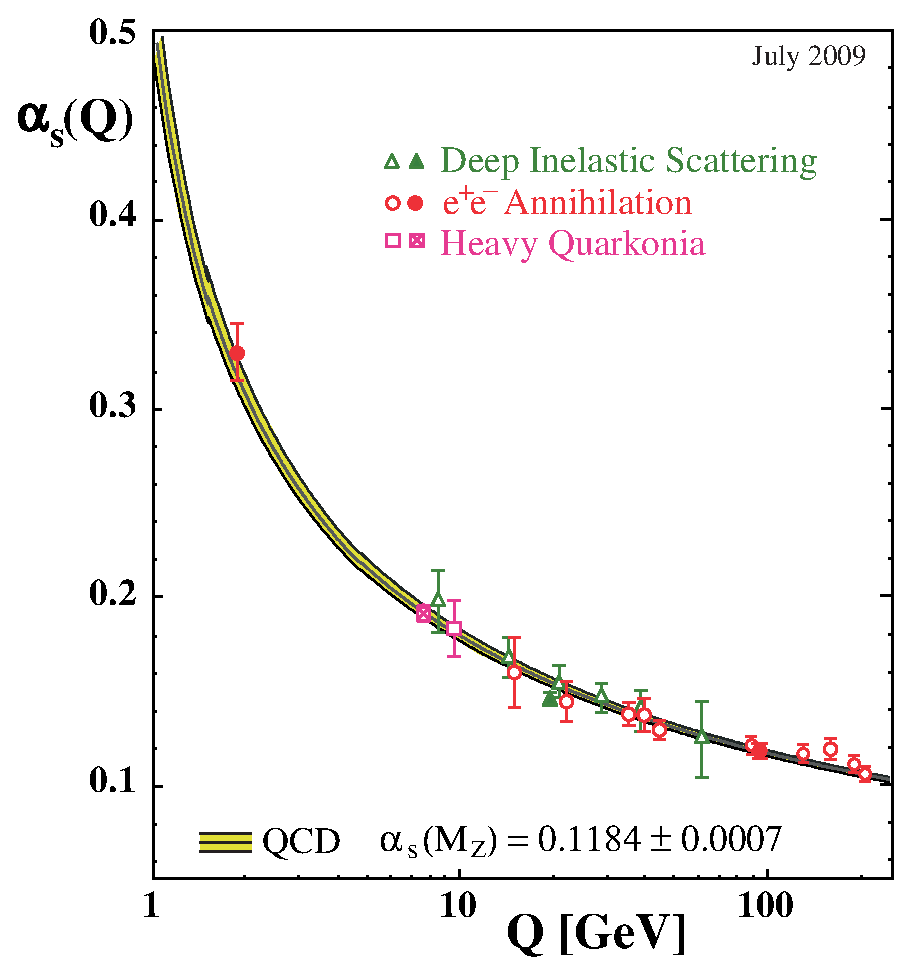
\includegraphics[width=0.795\textwidth]{StandardModel/Figures/asq-2009.eps}
    }
  \end{center}
  \caption[Measurement of $\alpha_s(Q)$~\cite{Bethke:2009jm}.]{Measurement of $\alpha_s(Q)$~\cite{Bethke:2009jm}.}
  \label{fig:alphaRunning}
\end{figure}

\begin{equation}
\mu_{R}^{2} \frac{d\alpha_s(\mu_{R}^{2})}{d\mu_{R}^{2}} = -(33 - 2n_{f})\alpha_{s}^{2}(\mu_{R}^{2}),
\label{eq:RGE_QCD}
\end{equation}

\noindent where $\alpha_{s}(\mu_R)$ is the coupling as a function of an (unphysical) renormalization scale $\mu_R$, and $n_f$ is the number of families or generations.

The minus sign in the previous equation has its origin in the gluon self-interaction and leads to the two main characteristic properties of QCD: \emph{asymptotic freedom} and \emph{confinement}.
The integration of Equation \ref{eq:RGE_QCD} shows that at very high energies or equivalently, at very short distances the strong interaction coupling is weak.
This situation is called asymptotic freedom and is totally supported by the results from deep inelastic scattering (DIS) experiments (described in the next section).
Therefore, inside hadrons, the quarks behave as almost being free particles. 
In the $\unit[100]{GeV}$-$\unit[1]{TeV}$ energy range, $\alpha_s\sim 0.1$, and perturbation theory can be applied to QCD (pQCD).

This equation also shows that the coupling constant asymptotically diverges at low energies (large distances), making therefore impossible to produce isolated quarks.
When in a $q\bar{q}$ pair, the quarks begin to separate from each other, the energy of the field between them increases.
At some point, it is energetically favorable to create an additional $q\bar{q}$ pair, so at the end, there are only colorless bound states (hadrons).
This situation is called color confinement and it is related to the process of jet formation (Section~\ref{subsec:HadronizationModels}).


\section{Deep Inelastic Scattering}
    \label{sec:DIS}

\subsection{Probing the proton}
    \label{subsec:ProvingProton}

Deep Inelastic Scattering (DIS) experiments have been performed since the 1960's to study the internal structure of nucleons.
Electrons with energies up to $\unit[20]{GeV}$ were sent against a target of hydrogen:

\begin{equation}
e + P \rightarrow e + X,
\label{eq:DISschema}
\end{equation}

\noindent where $P$ is the proton and $X$ is any hadronic final state (Figure~\ref{fig:DISexample}).

\begin{figure}[!t]
  \begin{center}
    \mbox{
        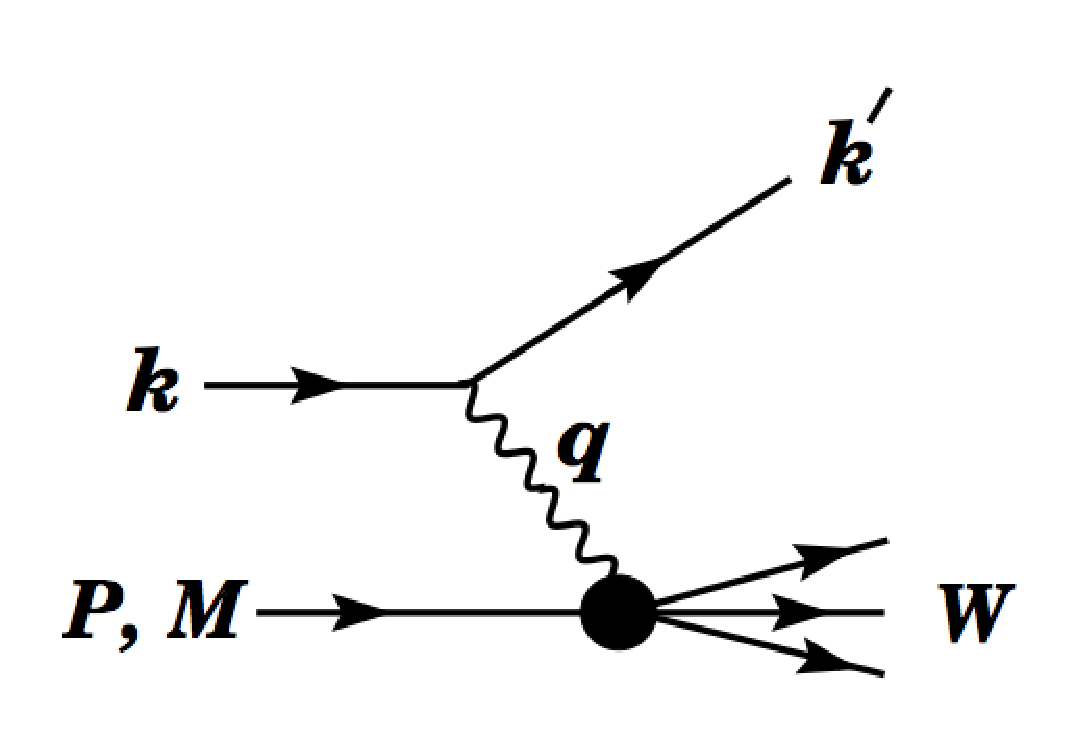
\includegraphics[width=0.495\textwidth]{StandardModel/Figures/DISexample.eps}
    }
  \end{center}
  \caption[Kinematic quantities for the description of the Deep Inelastic scattering.]{Kinematic quantities for the description of deep inelastic scattering. The quantities $k$ and $k'$ are the four-momenta of the incoming and outgoing leptons, $P$ is the four-momentum of a nucleon with mass $M$, and $W$ is the mass of the recoiling system $X$. The exchanged particle is a $\gamma$, $W^{\pm}$, or $Z$; it transfers four-momentum $q = k - k^{\prime}$ to the nucleon. \protect\cite{Beringer:1900zz}}
  \label{fig:DISexample}
\end{figure}

The kinematics of DIS can be described by the variables:

\begin{equation}
Q^2 \equiv -q^2 = (k-k')^2 \qquad\qquad x = \frac{Q^2}{2(P \cdot q)},
\label{eq:DISvariables}
\end{equation}

\noindent where $k$ and $k'$ are the four momentum of the incoming and outgoing electrons, $P$ is the momentum of the incoming proton and $x$ is interpreted as the fraction of the proton momentum carried by the interacting quark.

In the first DIS experiments, a larger number of large-angle deflected electrons than expected was found.
A phenomenological explanation to these results was given, considering the proton to be composed of non-interacting point-like particles, called \emph{partons}.
Therefore, $eP$ collisions can be regarded as ``hard'' interactions between the electron and partons inside the proton.
The Parton Model considers nucleons as bound states of three partons, each carrying a fraction $x$ of the total nucleon momentum such that:

\begin{equation}
\sum_{\text{partons}}{x_p} = 1.
\label{eq:sumFractionProton}
\end{equation}

In the parton model, the total cross section can be expressed in terms of electron-parton $ep$ interaction cross section:

\begin{equation}
\sigma(eP\rightarrow eX) = f \otimes \sigma(ep\rightarrow ep),
\label{eq:FactorizationTheoremSketch}
\end{equation}

\noindent where $f$ is the parton density, also called parton distribution function (PDF).
The term $f_i(x)dx$ gives the probability of finding a parton of type $i$ in the proton carrying a fraction between $x$ and $x+dx$ of the proton total momentum.
A prediction of the parton model is that, in the infinite-momentum frame of the proton, where $Q^2 \rightarrow \infty$ and the transverse momentum of the partons inside the proton are small, the parton densities are only a function of $x$.
This behavior is called Bjorken scaling.

However, in QCD, the radiation of gluons from the quarks leads to a violation of the scaling predicted by the Parton Model.
In particular, the DIS cross section can be written as:

\begin{equation}
\frac{d^2\,\sigma (e^{\pm}P)}{dx\,dQ^2} = \frac{4\pi\alpha^2}{xQ^4} \left( y^2 x F_1(x, Q^2) + (1-y) F_2(x, Q^2) \mp y(1-y)x F_3(x, Q^2) \right)
\label{eq:DISxsection}
\end{equation}

\noindent where $y = \frac{Q}{sx}$ and $F_i$ are the proton structure functions defined as:

\begin{equation}
F_1 = \frac{1}{2}\sum_i{e_i^2 f_i} \qquad \qquad F_2 = \frac{1}{2}\sum_i{e_i^2 x f_i},
\label{eq:DISformfactors}
\end{equation}

\noindent that explicitly depend on $Q$, and $F_3$ is found to be zero in parity conserving photon exchanges.
The reason for this dependence is that, an increase in $Q^2$ allows the gluons exchanged by the quarks (and their subsequent splittings into $q\bar{q}$ pairs) to be better resolved by the photon.
Figure~\ref{fig:ProtonPDFs} shows the parton distribution functions of a proton measured at different values of $Q^2$.
Valence quarks dominate for large values of $x$ (they carry the biggest fraction of the total proton momentum), while gluons and sea quarks dominate at low $x$. 
This figure also shows that as $Q^2$ increases, the probability for finding gluons and sea quarks at low $x$ values is higher.

\begin{figure}[!ht]
  \begin{center}
    \mbox{
        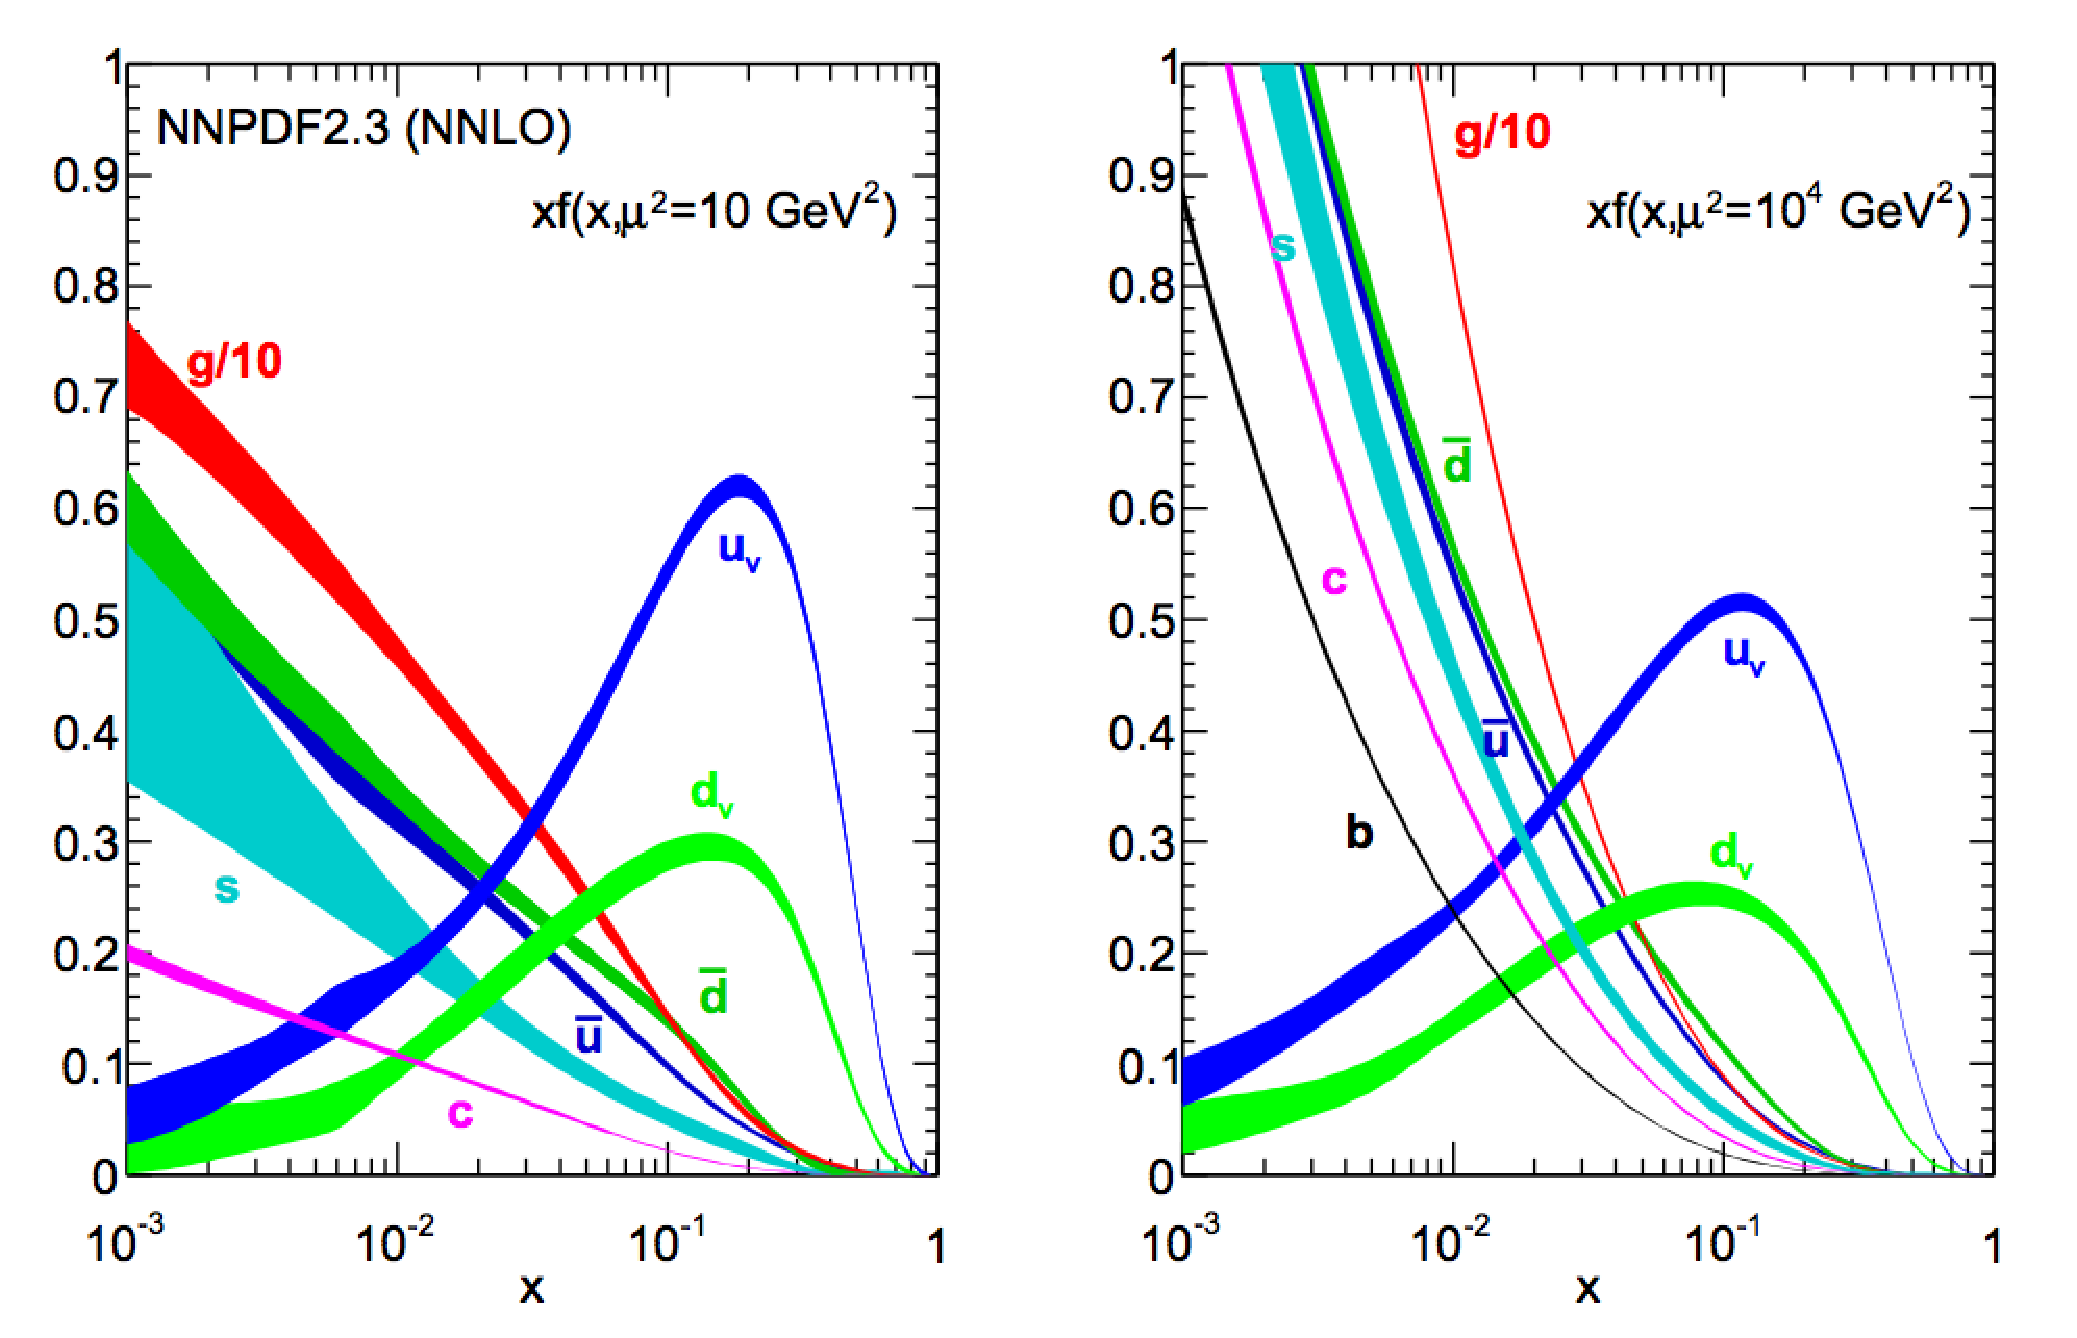
\includegraphics[width=0.995\textwidth]{StandardModel/Figures/ProtonPDF.eps}
    }
  \end{center}
  \caption[Distributions of the parton distribution functions $xf(x)$.]{Distributions of the parton distribution functions $xf(x)$ (where $f = u_v,\, d_v,\, \bar{u},\, \bar{d},\, s \approx \bar{s},\, c=\bar{c},\, b=\bar{b}$) obtained in NNLO \texttt{NNPDF2.3} global analysis at scales $\mu^2 = \unit[10]{GeV^2}$ and $\mu^2 = \unit[10^4]{GeV^2}$, with $\alpha_s(M_Z) = 0.118$. \protect\cite{Beringer:1900zz}}
  \label{fig:ProtonPDFs}
\end{figure}


\subsection{Parton Distribution Function}
    \label{subsec:PDF_proton}

The partonic description of the hadrons that are collided determines the theoretical predictions on high energy physics.
Perturbative QCD cannot predict the form of the PDFs, but can describe their evolution with the variation of the scale $Q^2$:

\begin{equation}
\begin{split}
\frac{d}{d\log{Q^2}}f_{q}(x, Q^2) = \frac{\alpha_s}{2\pi}\int_{x}^{1}{\frac{dy}{y}\,f_{q}(y, Q^2)\,P_{qq}\left(\frac{x}{y}\right) + f_{g}(y, Q^2)\,P_{qg}\left(\frac{x}{y}\right)} \\
\frac{d}{d\log{Q^2}}f_{g}(x, Q^2) = \frac{\alpha_s}{2\pi}\int_{x}^{1}{\frac{dy}{y}\,f_{q}(y, Q^2)\,P_{gq}\left(\frac{x}{y}\right) + f_{g}(y, Q^2)\,P_{gg}\left(\frac{x}{y}\right)}.
\end{split}
\label{eq:EvolutionPDF}
\end{equation}

\noindent where $P_{ab}(z)$ are the Dokshitzer-Gribov-Lipatov-Altarelli-Parisi (DGLAP) splitting functions, that describe the probability that a parton of type $b$ radiates a quark or a gluon of type $a$, carrying a fraction $z$ of the initial's parton momentum.
In particular, the first expression describes the change of the quark densities with $Q^2$ due to gluon radiation and gluon splitting, while the second expression describes the change of the gluon densities with $Q^2$ due to gluon radiation from quarks and gluons.
The DGLAP splitting functions at the lowest order in $\alpha_s$, in the small angle approximation and averaging over the polarizations and spins are expressed as~\cite{Halzen}:

\begin{equation}
\begin{split}
&P_{qq}(z) = \frac{4}{3}\frac{1+z^2}{1-z}, \\
&P_{gq}(z) = \frac{4}{3}\frac{1+(1-z)^2}{z}, \\
&P_{qg}(z) = \frac{1}{2}\left(z^2+(1-z)^2\right), \\
&P_{gg}(z) = 6\left(\frac{1-z}{z} + \frac{z}{1-z} + z(1-z)\right).
\end{split}
\label{eq:DGLAP}
\end{equation}


\subsection{PDF parametrization}

Experimental data are fitted to obtain the parton densities at a given scale $Q^2$, and the evolution equations \ref{eq:EvolutionPDF} are used to predict the PDFs at different scales.
Figure~\ref{fig:DIS_F2fit} shows the structure function $F_2$ as a function of $x$ and $Q^2$ as measured from DIS and fixed target experiments, and the evolution predicted with the DGLAP equations.
The structure function $F_2$ shows no dependence on $Q^2$ for large values of $x$.
However, as $x$ decreases, the effect of the gluons and sea quarks start to be important, thus violating the Bjorken scaling.

\begin{figure}[!t]
  \begin{center}
    \mbox{
        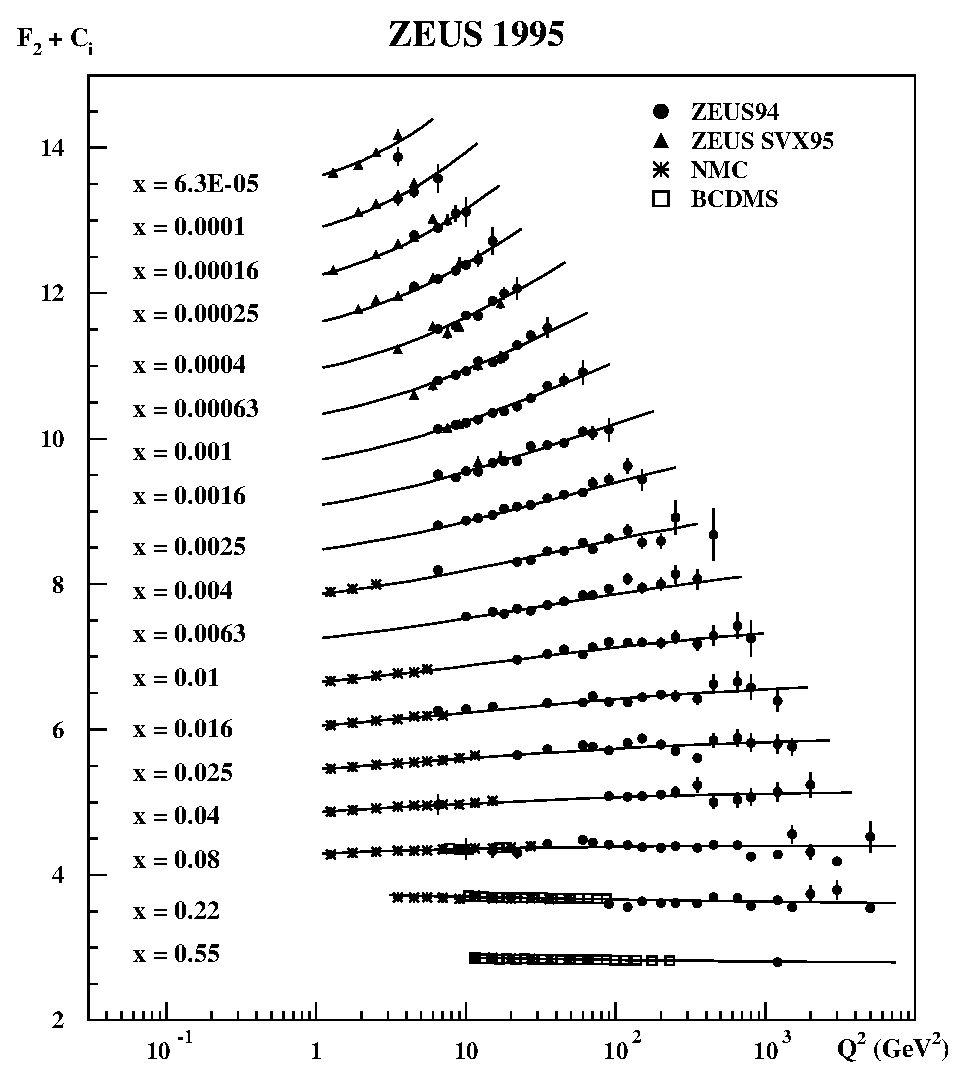
\includegraphics[width=0.995\textwidth]{StandardModel/Figures/StructureFunctionZEUS.eps}
    }
  \end{center}
  \caption[The proton structure function $F_2$ versus $Q^2$ at fixed values of $x$.]{The proton structure function $F_2$ versus $Q^2$ at fixed values of $x$. Data are from the ZEUS94 and SVX95 analyses and from the NMC and BCDMS fixed target experiments. For clarity an amount $C_i = 13.6-0.6i$ is added to $F_2$ where $i=1$ (18) for the lowest (highest) $x$ value~\cite{Breitweg:1998dz}.}
  \label{fig:DIS_F2fit}
\end{figure}

The PDFs are expected to be smooth functions of the scaling variable $x$, and can be parametrized.
In this analysis, the parametrization provided by the CTEQ~\cite{Lai:1994bb}, CT10~\cite{Lai:2010vv} and MSTW~\cite{Martin:2009iq} collaborations are used.
As an example, the CT10 parametrizaton used for the quarks and the gluon parton densities is:

\begin{equation}
xf_i(x, Q^2_0) = A_0 \cdot x^{A_1}(1-x)^{A_2}\exp{(A_3x + A_4 x^2 + A_5\sqrt{x})},
\label{eq:parametrizationPDF}
\end{equation}

\noindent where $f_i$ is a particular parton density at $Q^2_0$ and $A_i$ are the parameters to be fitted, obtained with a $\chi^2$ parametrization over data from different types of measurements.
Not all these parameters are free, since these functions must satisfy flavor and momentum sum rules.


\section{Monte Carlo simulation}
    \label{sec:MCSimulation}

Monte Carlo (MC) codes are tools that enable the description of the final states resulting from high-energy collisions, where the state-of-the-art knowledge about QED and QCD is implemented by using MC techniques.
They have been developed to help interpreting the data from high energy particle colliders in order to extract the measurement of fundamental physical parameters or to infer the possible existence of new physics beyond the SM.
The next subsections are devoted to describe the different phases of a MC event generation~\cite{Skands:2011pf,ellis2003qcd}.
Figure~\ref{fig:HardCollisionEvolution} shows the general structure of a hard proton-proton collision.
The dotted circle {\em H} separates the perturbative QCD (hard process, initial and final state radiation) from non-perturbative contributions (underlying event, hadronization and PDFs).
%Finally, a summary of the characteristics of the MC generators used in the analysis presented will be shown.

\begin{figure}[!ht]
  \begin{center}
    \mbox{
        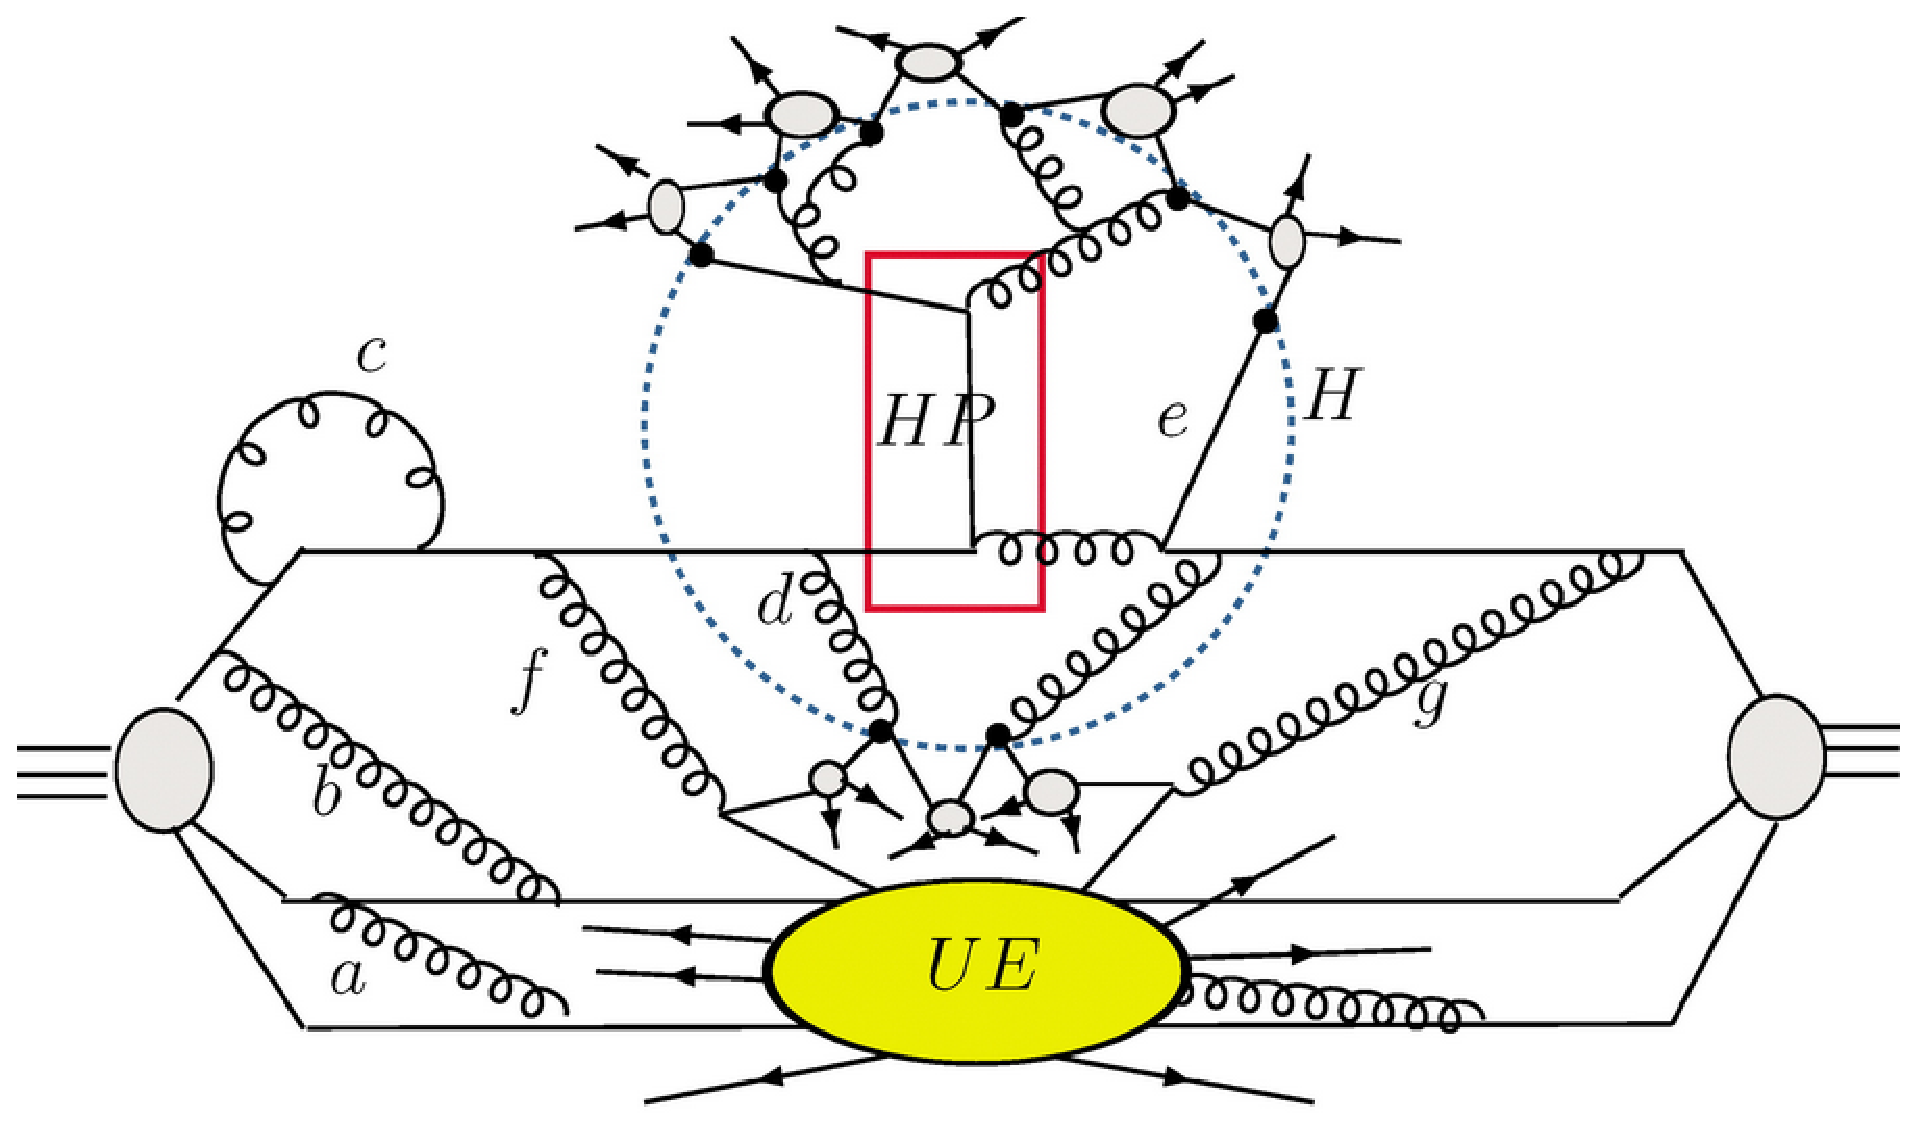
\includegraphics[width=0.995\textwidth]{StandardModel/Figures/HardInteractionEvolution.eps}
    }
  \end{center}
  \caption[General structure of a hard proton-proton collision.]{General structure of a hard proton-proton collision. HP, denotes the hard process, and UE, is the underlying event~\protect\cite{Mangano:2005dj}.}
  \label{fig:HardCollisionEvolution}
\end{figure}


\subsection{Parton-level event generators}
    \label{subsec:EventGenerators}

The cross section for a two-hadron interaction with momenta $P_1$ and $P_2$, can be factorized into short- and long-distance effects delimited by a factorization scale $\mu_F$, according to the factorization theorem:

\begin{equation}
\begin{split}
\sigma(P_1, P_2) = \sum_{i, j} \int dx_1\, dx_2\, f_i(x, \mu_F^2)\, f_j(x, \mu_F^2) \\
  \times\; \hat{\sigma}_{ij}(p_1, p_2, \alpha_s(\mu_R^2), Q^2/\mu_F^2,  Q^2/\mu_R^2) 
\end{split}
\label{eqXSecQCDComputation}
\end{equation}

\noindent where $f_i$ are the PDFs of each interacting parton, the sum runs over all parton types, and $\hat{\sigma}_{ij}$ is the parton cross section for incoming partons with momenta $p_1=x_1P_1$ and $p_2=x_2P_2$, respectively.
As long as the same factorization scale is used, the same PDFs extracted from DIS experiments can be used for $ep$, $\pp$ and $\ppbar$ experiments.
$\hat{\sigma}_{ij}$ is calculated at a given order on pQCD, which introduces a dependence on a renormalization scale $\mu_R$, that is usually chosen to be equal to $\mu_F$.

Schematically, the all-orders partonic cross section, $\hat{\sigma}_{ij}$ for a given process $F$, with any extra emission, can be expressed as:

\begin{equation}
\begin{split}
\hat{\sigma}_{ij} &= \int{d\mathcal{O}\; \frac{\hat{\sigma}_{ij}}{d\mathcal{O}}} \\
                  &= \int{d\mathcal{O}} \; \underbrace{\sum_{k=0}^{\infty}{\int{d\Phi_{F+k}}}}_{\Sigma\text{ legs}}
                                          |\underbrace{\sum_{\ell=0}^{\infty}{\mathcal{M}^{\ell}_{F+k}} }_{\Sigma \text{ loops}}|^2 \delta(\mathcal{O} - \mathcal{O}(\Phi_{F+k})) ,
\end{split}
\label{eq:AllOrdersXSection}
\end{equation}

\noindent where the sum over $k$ represents the sum over additional ``real emission'' corrections, called legs, and the sum over $\ell$ represents the sum over additional virtual corrections, loops.
$\Phi_{F+k}$ represents the phase space of the configuration with $k$ legs and $\ell$ loops.

The various fixed order truncations of pQCD can be recovered by limiting the nested sums in Equation~\ref{eq:AllOrdersXSection} to include only specific values of $k+\ell$.
Therefore,

\begin{itemize}
\item $k=0$, $\ell=0$: Leading order (usually tree-level) for inclusive $F$ production.
\item $k=n$, $\ell=0$: Leading order for $F+n$~jets.
\item $k+\ell \leq n$: N$^n$LO for $F$ (includes N$^{n-1}$LO for $F+1$ jet,  N$^{n-2}$LO for $F+2$ jets, and so on up to LO for $F+n$ jets).
\end{itemize}

The Kinoshita-Lee-Nauenberg (KLN) theorem~\cite{Kinoshita:1962ur,Lee:1964is} states that the divergences originated in the loops exactly cancel against those from the real emissions, order by order in perturbation theory.
However, in a fixed order calculation, e.g. leading order, in the situation for which $k\geq1, \ell=0$, the integration over the full momentum phase space will include configurations in which one or more of the $k$ partons become collinear or soft, thus leading to singularities in the integration region.
For this reason, the integration region needs to be modified to include only ``hard, well-separated'' momenta.
The remaining part of the phase space is then considered by the parton shower generators.


\subsection{Parton shower generators}
    \label{subsec:PartonShowerGenerators}

As already mentioned, the fixed order calculations introduced in the previous section are only valid if two conditions are fulfilled:

\begin{enumerate}
\item The strong coupling, $\alpha_s$, is small, so that perturbation theory is valid.
\item The phase space region is restricted to configurations in which real emissions are ``hard and well-separated''.
\end{enumerate}

Parton showers are included in the MC simulations to approximately account for the rest of higher order contributions to emulate a complete final state.
By the successive parton emission, the partons in the final state produce a cascade, where the splitting functions (Eq.~\ref{eq:DGLAP}) govern the radiation process.
A parton shower generator simulates the successive emission of quarks and gluons from the partons in the final (or initial) state.
This simulation is approximate, since it assumes completely independent parton emissions, neglects any interference term among them and does not consider virtual corrections.
In the almost-collinear splitting of a parton, the $n+1$-parton differential cross-section can be related to the $n$-parton cross section before splitting as

\begin{equation}
d\sigma_{n+1} \approx d\sigma_n \; dP_i(z,\mu^2)
\label{eq:PSrelation}
\end{equation}

\noindent where

\begin{equation}
dP_i(z,\mu^2) = \frac{d\mu^2}{\mu^2} \; \frac{\alpha_s}{2\pi} \; P_{ji}(z)dz 
\label{eq:dPi}
\end{equation}

\noindent shows the probability that parton $i$ will split into two partons at a virtuality scale $\mu$ and with parton $j$ carrying a fraction $z$ of the $i$'s parton momentum and $P_{ji}(z)$ are the same DGLAP equations from Eq. \ref{eq:DGLAP}.
This relation is universal, so for any process involving $n$ partons, this equation can be applied to obtain an approximation for $\sigma_{n+1}$.
This probability diverges logarithmically in the soft ($z=1, 0$) and collinear ($\mu = 0$) regions, which can be understood as a consequence of the non-perturbativity of QCD at low scales.
These divergences are not a problem because detectors will not be able to resolve two partons very close one another, thus introducing an effective cutoff to screen these regions.

The quality of the approximation from Equation~\ref{eq:dPi} is governed by how many terms besides the leading one shown in this equation are included.
Including all possible terms, the most general form for the cross section of the process $F + n$ jets, restricted to the phase-space region above some infrared cutoff scale, has the following algebraic structure:

\begin{equation}
\sigma_{F+n} = \alpha_s^n (\ln^{2n} + \ln^{2n-1} + \ln^{2n-2} + \cdots + \ln + \mathcal{R}),
\label{leadinglogapproximation}
\end{equation}

\noindent and therefore, the simplest approximation one can build from this equation is the ``leading-logarithmic'' (LL), in which all the terms of the series are dropped but the $\ln^{2n}$ one.

For the computer implementation of the parton shower, the Monte Carlo programs use Sudakov form factors:

\begin{equation}
\Delta_i(q_1^2, q_2^2) = \exp{\left( - \sum_{j} \int_{q_2^2}^{q_1^2}{\,\int_{z_\text{min}}^{z_\text{max}}{dP_i(z',dq'^2)}} \right)},
\label{eq:Sudakov}
\end{equation}

\noindent derived from the splitting functions.
The Sudakov form factors represent the probability that a parton evolves from an initial scale $q_1$ to a lower scale $q_2$ without branching.

To simplify the implementation of the calculations in the Monte Carlo programs, the radiations are separated into initial-state and final-state showers, depending on whether they start off an incoming or outgoing parton of the hard scattering.
In the final-state showers, the Monte Carlo branching algorithm operates in steps:

\begin{enumerate}
\item When a branching $a\rightarrow b + c$ occurs at scale $q_a$, the fraction of momentum carried by the daughter partons $x_b/x_a$ is determined using the appropriate splitting function $P_{ab}$, and the opening angle $\theta_a$ between $b$ and $c$ is given by $q_a = E_a^2(1-\cos{\theta_a})$.

\item The scale at which the partons $b$ and $c$ will branch is determined with the Sudakov factors.
Since the scale $q_a$ is proportional to the virtual mass, $q_b$ and $q_c$ are kinematically constrained to satisfy $\sqrt{q_a} > \sqrt{q_b} + \sqrt{q_c}$, thus imposing that the subsequent branchings on the daughter partons will have smaller opening angles.

\item The shower is terminated when these virtualities have fallen to the hadronization scale, $Q^2\sim\unit[1]{GeV}$.
\end{enumerate}

In the initial state showers, the same algorithm is applied, but operated backwards in time.
Starting from an incoming parton at the hard interaction $b$, it finds the branching $a\rightarrow b+c$, where $c$ can further branch in a final-state fashion.
Therefore, in the construction of the initial-state shower, the fraction of momentum $x$ is increased, and at the end it will match that described by the PDFs.


\subsection{Matrix element and parton shower matching}
    \label{subsec:MEandPSmatching}

The addition of the parton shower to the parton-level event generator can introduce double-counting of events in some regions of the phase space.
This is illustrated in a very simple way in Figure~\ref{fig:MatchingOverlap}.
The LO cross section for some process (green area), $F$, with a LL shower added to it (yellow area), is found in the left-pane of this figure.
To improve the description of the $F+1$ process from LL to LO, one needs to add the actual LO matrix element for $F+1$ (with a LL parton shower description as well).
However, the LO matrix element for $F+1$ is divergent, and therefore, only the phase-space region with at least one hard resolved jet can be covered (illustrated by the half shaded boxes in the middle pane of Figure~\ref{fig:MatchingOverlap}).
When one adds these two samples, the LL terms of the inclusive cross section for $F+1$ are counted twice, once from the shower of $F$, and once from the matrix element for $F+1$, illustrated by the red areas of the right-hand pane of Figure~\ref{fig:MatchingOverlap}.

\begin{figure}[!ht]
  \begin{center}
    \mbox{
        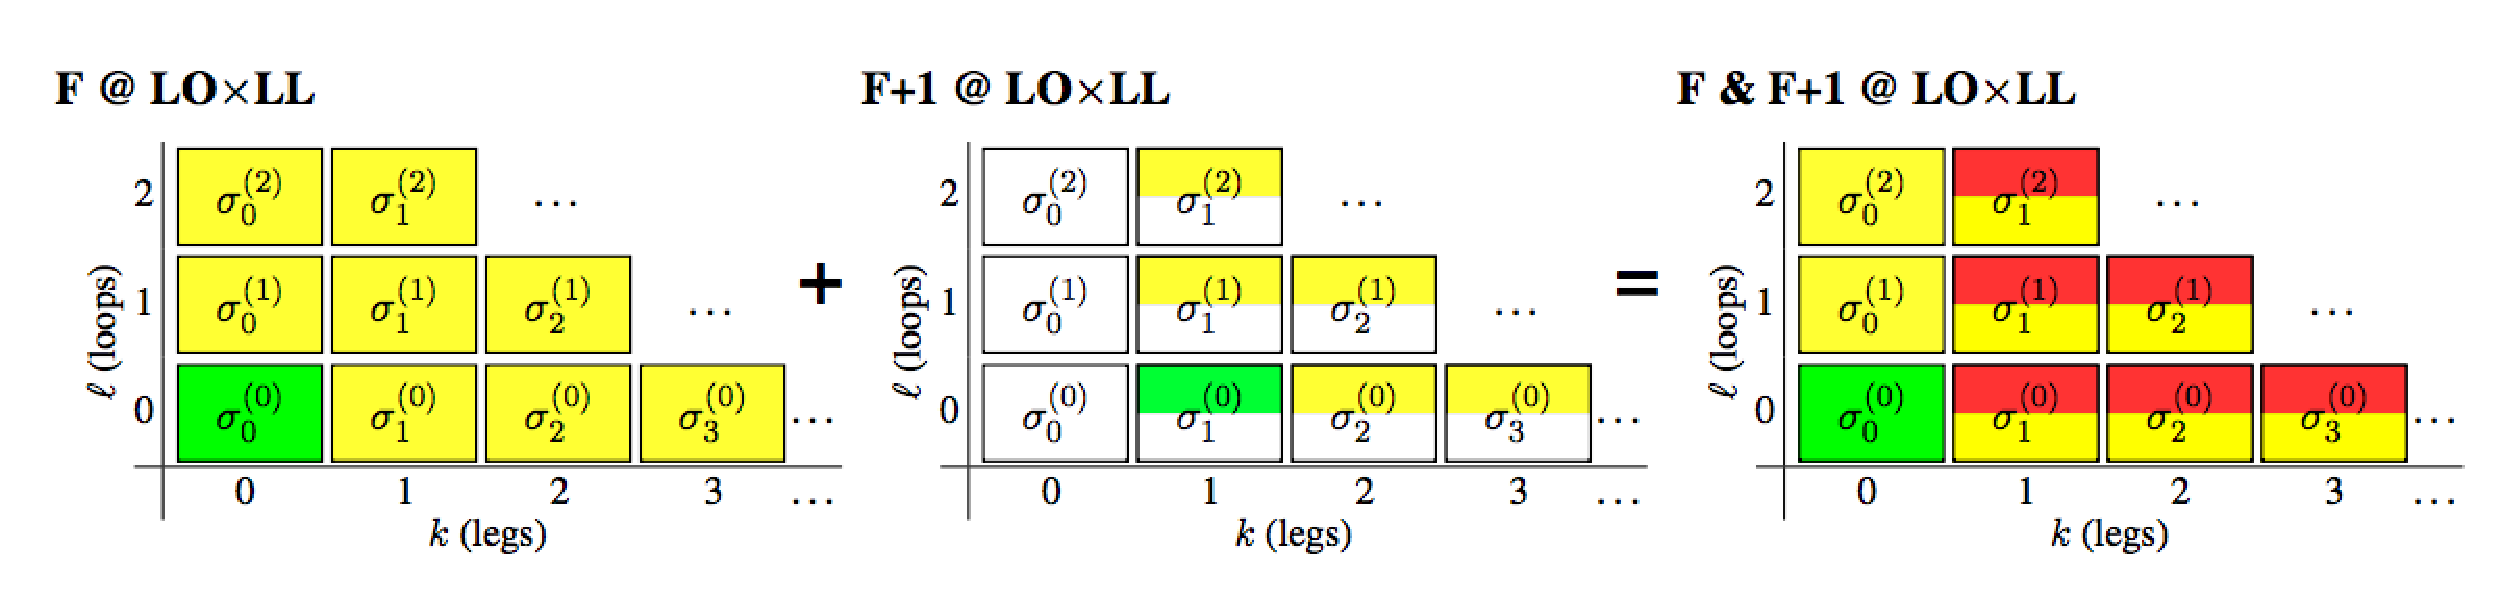
\includegraphics[width=0.995\textwidth]{StandardModel/Figures/MatchingMCOverlap.eps}
    }
  \end{center}
  \caption[Double-counting problem caused by adding cross sections involving matrix elements with different numbers of legs]
{Illustration of the double-counting problem caused by naively adding cross sections involving matrix elements with different numbers of legs~\cite{Skands:2011pf}.}
  \label{fig:MatchingOverlap}
\end{figure}

To remove this overlap, the phase space covered by the matrix element calculation, and the space covered by the parton shower evolution needs to be separated.
There are two main matching schemes: the Catani-Krauss-Kuhn-Webber (CKKW \cite{Catani:2001cc}) and the Michelangelo L. Mangano (MLM \cite{Mangano:2006rw}) methods.
They separate the phase space into the ME and PS regions by introducing resolution parameters that distinguish between resolved and non-resolved jets, to be described by the ME and the PS, respectively.

In the CKKW algorithm, a parton branching history is generated using the \kt{} algorithm \cite{Catani:1991hj}, given a configuration with $n$ partons in the final state.
The values of $\alpha_s$ in every vertex of the branching, and the Sudakov factor from every line between the vertices, are used to reweight the matrix elements.
The initial conditions of the shower are then set to have a smooth transition between the reweighted matrix elements and the parton shower, where the hard emissions in the shower evolution are vetoed if they have enough transverse momentum to produce a separate jet, according to the \kt{} algorithm.

The matching MLM procedure starts by separating the events in exclusive samples of $n$ partons in the final state, and then, the parton shower is developed in that event using a PS Monte Carlo.
The parton configuration after the showering is then processed with a cone jet algorithm, with a radius $R_{\text{jet}}$.
Then, the original $n$ partons are matched to the jets if $\Delta R(\text{jet}, \text{parton}) < R_{\text{jet}}$.
If all the partons are matched to a jet and there are no extra jets, i.e. $N_{\text{jets}}=n$, the event is accepted.
Otherwise, the event is rejected to avoid further hard emissions that would lead to additional jets.
Finally, the events with different jet multiplicities, $n=0, 1, 2, \ldots, k$, are recombined in a single sample.
The events in the sample with parton multiplicities higher than $k$ jets are accepted if $N_\text{jets}\geq k$.


\subsection{Hadronization models}
    \label{subsec:HadronizationModels}

As the collision process evolves and the partons radiate and travel further apart, the QCD running coupling increases as the values of the shower evolution scale $Q^2$ decrease.
Therefore, the confining effects of QCD become important and the dynamics enter a non-perturbative phase which leads to the formation of the observed final-state hadrons.
Event generators have to rely on models based on general features of QCD.

As a consequence of the factorization assumption and color preconfinement, the hadronization of the partons is independent of the hard scattering process.
Therefore, the parameters of a model used to describe a hadronization can be fitted to the results of one experiment and then applied to another.

The most used hadronization models are the string fragmentation and the cluster hadronization models, which are described below.

\begin{figure}[!ht]
  \begin{center}
    \mbox{
        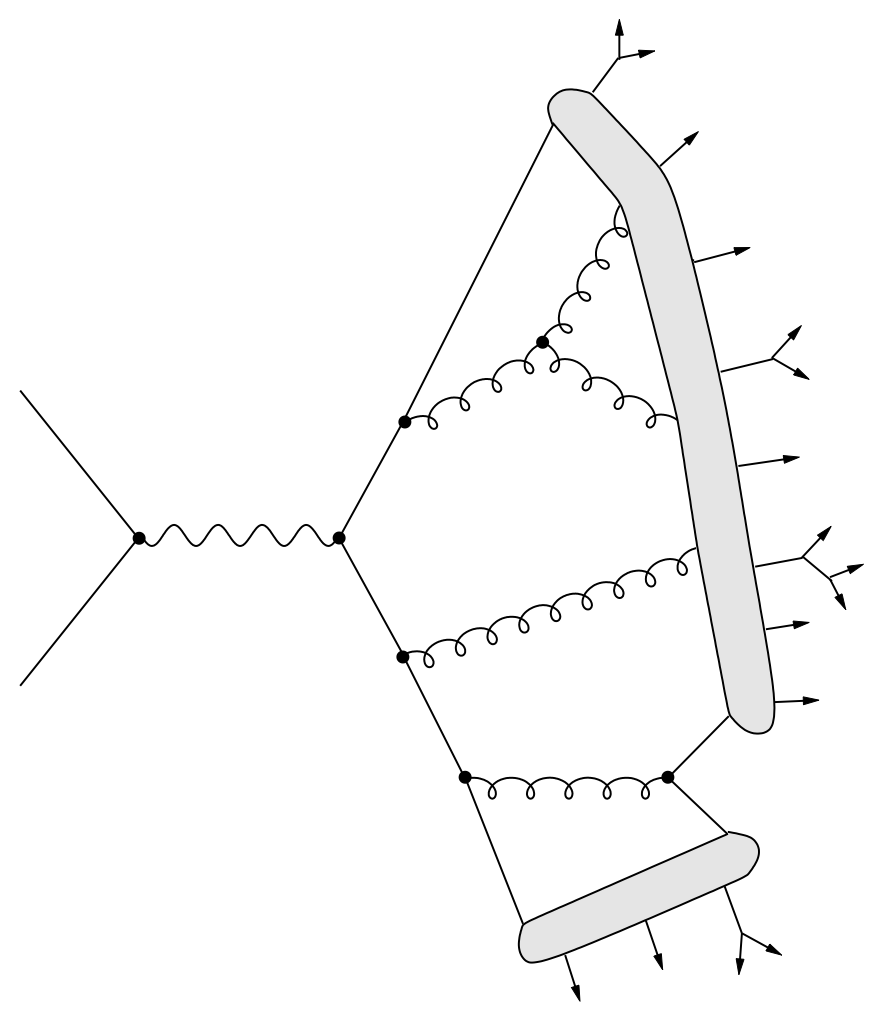
\includegraphics[width=0.495\textwidth]{StandardModel/Figures/HadronizationString.eps}
        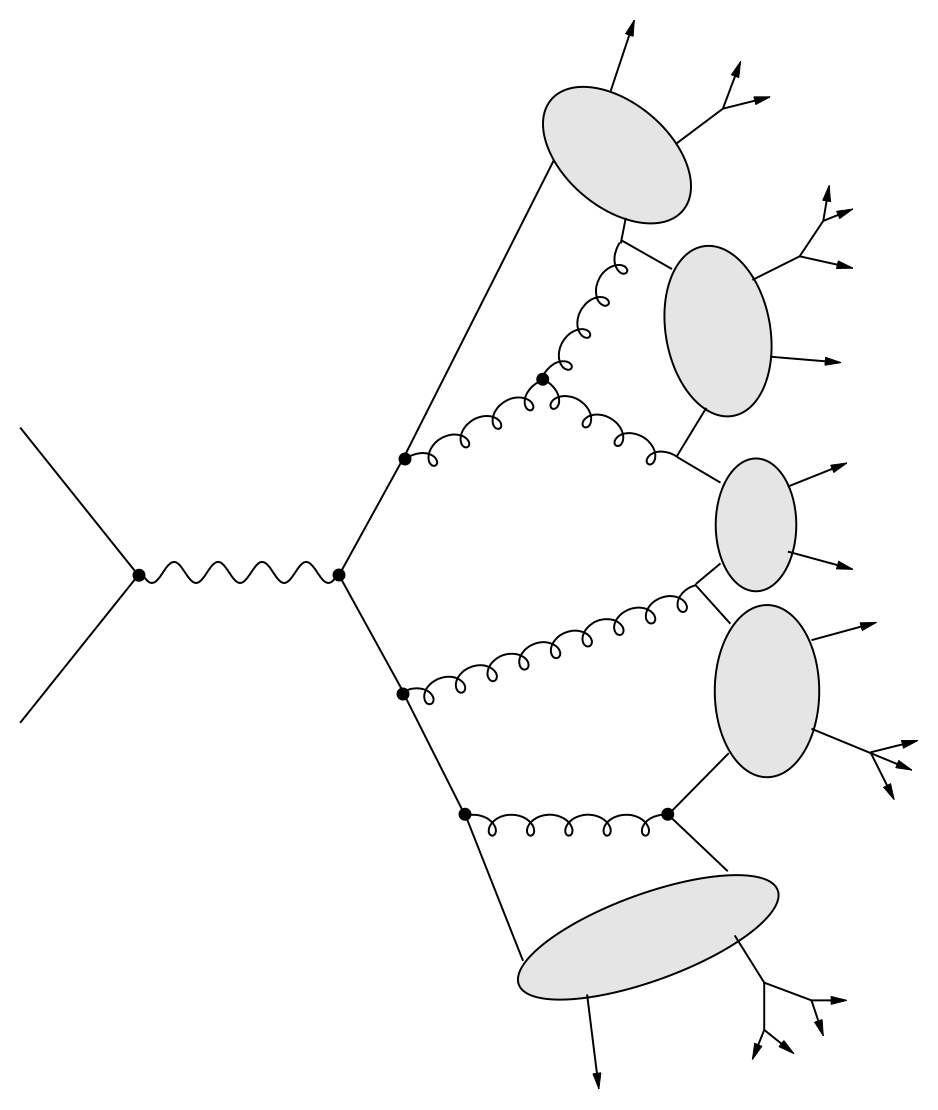
\includegraphics[width=0.495\textwidth]{StandardModel/Figures/HadronizationCluster.eps}
    }
  \end{center}
  \caption[Illustration of different hadronization models.]{Illustration of string fragmentation (left) and cluster hadronization (right) \protect\cite{Ellis:1991qj}.}
  \label{fig:HadronizationModels}
\end{figure}


\subsubsection{String fragmentation hadronization model}
    \label{subsubsec:StringModel}

The string model for hadronizaton, schematically shown in Figure \ref{fig:HadronizationModels} (left), uses string dynamics to describe the flux between a $q\bar{q}$ pair.
It is based on the observation that at large distances the potential energy of color sources increases linearly with their separation.
In the evolution of the hadronization process, the potential energy of the string increases as partons travel further apart at the expense of its kinetic energy.
When this energy becomes higher than the mass of a light $q\bar{q}$ pair, a new $q'\bar{q}'$ is created and the string breaks into two shorter strings creating two color-singlet states $q'\bar{q}$ and $q\bar{q}'$.
If the relative momentum of the new $q\bar{q}$ pairs connected to the same string is large enough, the string might break again.
Gluons act as ``kinks'' in the string, that add extra tension to it.
The creation of heavy quarks is suppressed during the hadronization as the production of light quark pairs ($u$, $d$ and $s$) is more energy favored.
The formation of baryons, 3-quark states, is achieved by considering them quark-diquark states, where diquarks are simply treated as antiquarks.


\subsubsection{Cluster hadronization model}
    \label{subsubsec:ClusterModel}

The cluser model is based on the color pre-confinement of the branching processes.
The process starts by splitting gluons that remain after parton shower into quark-antiquark pairs, so that only quarks are present.
They are then grouped in color-singlets.
The mass spectrum of these clusters peaks at low values of the order of the GeV, but has a broad tail at high masses.
The clusters decay typically into two hadrons.
Heavier hadrons are naturally suppressed by the mass spectra.
Furthermore, the heaviest clusters can decay into smaller clusters that subsequently decay into hadrons.
A sketch of this model is shown in Figure \ref{fig:HadronizationModels} (right).


\subsection{Underlying event}
    \label{subsec:UnderlyingEvent}

The underlying event (UE) refers to the interactions involving partons that do not directly take part in the hard scattering.
It cannot be described perturbatively because the interactions happen at low transferred momentum. 
These interactions also involve flavor and color connections to the hard scattering, and therefore they cannot be separated from the hard scattering in general.
The presence of particles originated in the UE can affect the interpretation of the data, for example, by contributing to the energy associated to the jets.
Phenomenological models~\cite{Butterworth:1996zw} are used to simulate the UE and are tuned to minimum bias data from hadron colliders~\cite{Sjostrand:2006za}.


\subsection{Monte Carlo generators}
    \label{subsec:MCgenerators}

A summary of the different MC generators used in this Thesis is presented in Table~\ref{tab:MCgenSummary}, and briefly discussed in the following sections~\cite{Buckley:2011ms, Aad:2010ah}.

\begin{table}[!ht]
  \begin{center}
    \begin{small}
      \setlength{\tabcolsep}{0.0pc}
      \begin{tabular*}{\textwidth}{@{\extracolsep{\fill}}ccccc}
        \noalign{\smallskip}\hline\hline\noalign{\smallskip}
        \textbf{Monte} & \textbf{Matrix}  & \textbf{ISR/} & \multirow{2}{*}{\textbf{Hadronization}} & \textbf{Underlying} \\
        \textbf{Carlo} & \textbf{element} & \textbf{FSR}  &                                         & \textbf{event} \\
        \noalign{\smallskip}\hline\noalign{\smallskip}
        \pythia{}      & LO               & Parton shower & String model  & Minimum bias \\
        \herwig{}      & LO               & Parton shower & Cluster model & \jimmy{}  \\
        \multirow{2}{*}{\sherpa{}}      & \multirow{2}{*}{LO}               & \pythia{}     & \multirow{2}{*}{\pythia{}}     & \multirow{2}{*}{\pythia{}} \\
         & & (CKKW matching)& & \\
        \multirow{3}{*}{\alpgen{}}      & \multirow{3}{*}{LO}               & \pythia{} or   & \multirow{3}{*}{\pythia{}}     & \multirow{3}{*}{\pythia{}} \\
         & & \herwig{}& & \\
         & & (MLM matching)& & \\
        \mcnlo{}       & NLO              & \herwig{} & \herwig{} & \herwig{} (\jimmy{})\\
        \multirow{2}{*}{\powheg{}}      & \multirow{2}{*}{NLO}               & \pythia{} or     & \pythia{} or     & \pythia{} or \\
         & & \herwig{} & \herwig{} & \herwig{} \\
        \multirow{2}{*}{\acer{}}      & \multirow{2}{*}{LO}               & \pythia{} or     & \pythia{} or     & \pythia{} or \\
         & & \herwig{} & \herwig{} & \herwig{} \\
        \multirow{2}{*}{\madgraph{}}      & \multirow{2}{*}{LO}               & \pythia{}     & \multirow{2}{*}{\pythia{}}    & \multirow{2}{*}{\pythia{}} \\
           & & (MLM matching) & &  \\
        \noalign{\smallskip}\hline\hline\noalign{\smallskip}
      \end{tabular*}
    \end{small}
  \end{center}
  \caption[Summary of the Monte Carlo generators used in the analysis.]{Summary of the Monte Carlo generators used in the analysis.}
  \label{tab:MCgenSummary}
\end{table}


\subsubsection{General purpose Monte Carlo generators}

\pythia{}~\cite{Sjostrand:2006za} and \herwig{}~\cite{Corcella:2000bw,Bahr:2008dy} are general purpose event generators that use matrix elements at leading-order in perturbation theory in QCD.
They are optimized to compute 2-to-1 and 2-to-2 processes, although 2-to-$n$ ($n>2$) processes can be achieved with initial- and final-state radiation, ordered in $\pt$ (angle) in the case of \pythia{} (\herwig{}).
For hadronization, \pythia{} uses the string model, while the cluster model is used in \herwig{}.
The latest is normally interfaced with \jimmy{}~\cite{Butterworth:1996zw} to model the underlying event. 


\subsubsection{Multi-leg Monte Carlo generators}

\sherpa{} \cite{Gleisberg:2008ta}, \alpgen{} \cite{Mangano:2002ea} and \madgraph{} \cite{Alwall:2011uj} are multi-purpose event generators, specialized in the computation of matrix elements involving 2-to-$n$ processes at LO in pQCD.
\madgraph{} and \alpgen{} compute separated ME up to $n=6$ and $n=9$, respectively.

In \sherpa{} the different jet multiplicities are generated in a single inclusive sample directly.
Parton showers and hadronizations are performed with either \pythia{} or \herwig{} for \alpgen{} and \sherpa{}, while \madgraph{} needs to be interfaced with \pythia{}.
The ME/PS matching is performed with the CKKW scheme in \sherpa{}, and with the MLM scheme in \alpgen{} and \madgraph{}.
Finally, \alpgen{} and \madgraph{} use \pythia{} to simulate the UE, while \sherpa{} uses its own implementation, closely following following the \pythia{} implementation.

In the analysis presented in the following chapters, \sherpa{} and \alpgen{} MC generators are used to model the $W/Z$+jets and the dibosons ($WW$, $ZZ$ or $WZ$) Standard Model processes.
The \madgraph{} interface, is instead used for the implementation of the new physics models.


\subsubsection{Next-to-leading order Monte Carlo generators}

\mcnlo{} \cite{Frixione:2008ym} and \powheg{} \cite{Frixione:2007vw} are event generators that use matrix elements at NLO in pQCD.
In the analysis, they are used to simulate processes involving the production of a top quark. 
\powheg{} is interfaced with either \pythia{} or \herwig{} for the modeling of the PS, hadronization or UE, while \mcnlo{} is interfaced with \herwig{}.

\cleardoublepage

\chapter{Beyond the Standard Model}
\label{chapter:BSM}

This chapter describes several extensions of the Standard Model.
These extensions aim to solve some of the many aspects of Nature that the SM cannot explain.
In particular, supersymmetry, the Arkani-Hamed Dvali Dimopoulos model of Large Extra Dimensions, and some models involving the production of Dark Matter will be covered in the following.


\section{Motivation to go beyond the Standard Model}
\label{sec:MotivationBSM}

The Standard Model provides the most successful description of the leptons, quarks and the interactions between them through the different bosons, as it was discussed throughout Chapter \ref{chapter:StandardModel}.
For the moment, no experiment besides the neutrino oscillations, that reveal the massive character of the neutrinos, has been able to find any clear deviation of the data with respect to the SM predictions.
However, there are a number of physical arguments that point to the existence of a theory that extends the SM in order to describe the physics at higher energies.

The first argument comes from the fact that gravity is not accommodated in the theory, thus preventing the Standard Model to be the Theory Of Everything (TOE), in which Nature could be described in a single framework.
For this reason, a new model is required at the reduced Planck scale $M_P = \left(8\pi G_\text{Newton}\right)^{-1/2} = \unit[2.4\times 10^{18}]{GeV}$, where the quantum gravitational effects are not negligible.

A further argument pointing to the need for new theories beyond the SM is the ``hierarchy problem'', regarded as a consequence of the fact that the ratio $M_P/M_W$ is so huge.
This is not a difficulty with the Standard Model itself, but rather a disturbing sensitivity of the Higgs potential to new physics in almost any imaginable extension of the SM.
Unlike the fermions and gauge bosons, spin-0 fields are not protected by any chiral or gauge symmetries against large radiative corrections to their masses.
In particular, in the SM there is no mechanism to prevent scalar particles from acquiring large masses through radiative corrections.
For this reason, the Higgs field receives enormous corrections from the virtual effects of any SM particle it couples to (see fermion loop diagram from Figure \ref{fig:HiggsLoop}).

\begin{figure}[!t]
\begin{center}
\mbox{
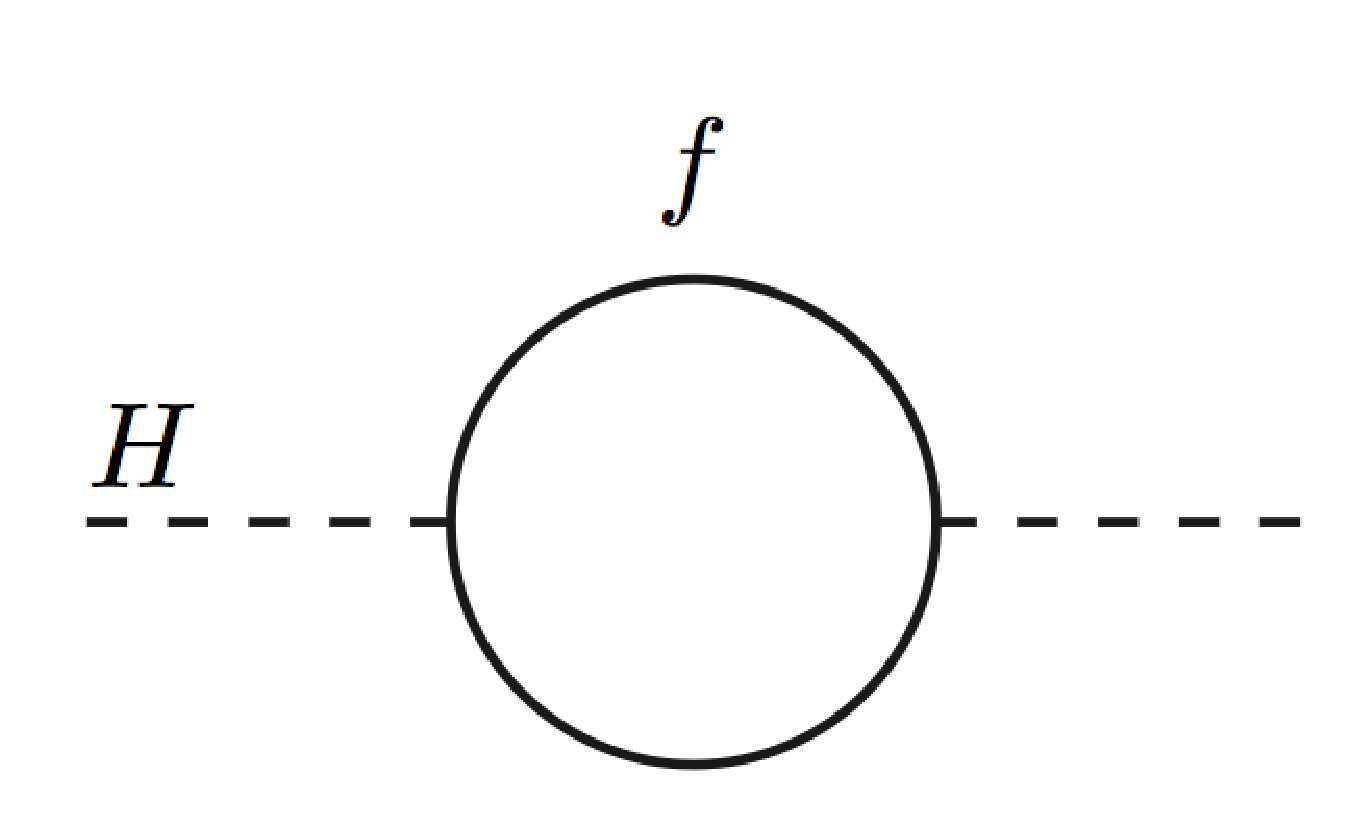
\includegraphics[width=0.495\textwidth]{BeyondSM/Figures/HiggsLoopFermion.eps}
%        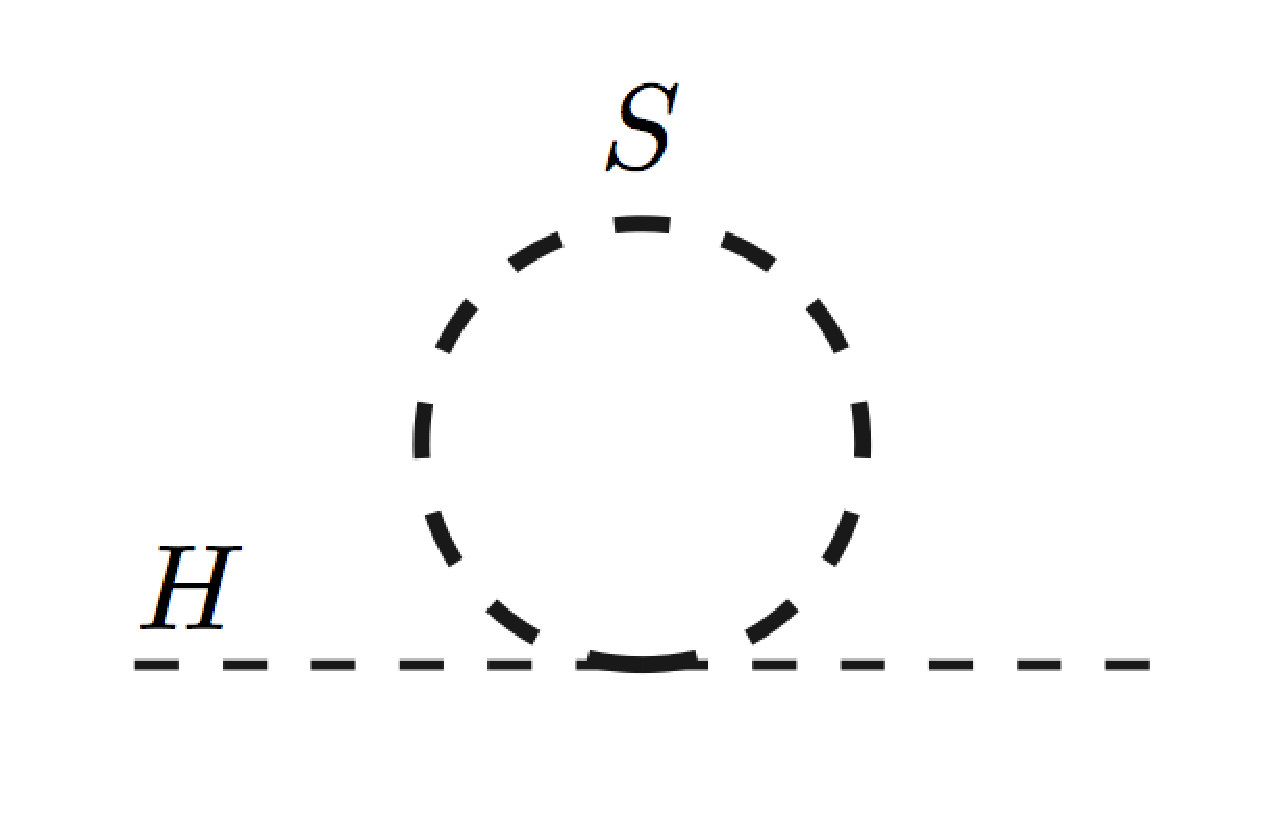
\includegraphics[width=0.495\textwidth]{BeyondSM/Figures/HiggsLoopScalar.eps}
}
\end{center}
\caption{One-loop quantum corrections to the Higgs mass due to fermions.}
\label{fig:HiggsLoop}
\end{figure}

Due to these corrections, the Higgs mass is:

\begin{equation}
m_{H_{\text{SM}}}^2 = (m_H)_{0}^{2} + \Delta m_H^2,
\label{eq:HiggsMassTotal}
\end{equation}

\noindent where $(m_H)_0$ is the bare Higgs mass and $\Delta m_H^2$ is the Higgs mass correction which, for the case of a fermion loop, is given by:

\begin{equation}
\Delta m_H^2 = -\frac{|\lambda_f|^2}{16\pi^2}\left[2\Lambda^2 + \mathcal{O}\left(m_f^2\ln{\left(\frac{\Lambda}{m_f}\right)}\right)\right],
\label{eq:HiggsMassCorrectionFermion}
\end{equation}

\noindent being $\lambda_f$ the Yukawa coupling of the fermion $f$ and being $\Lambda$ a cutoff.
The latter is interpreted as the energy scale at which new physics enters and the SM ceases to be valid.
If the SM needs to describe Nature up to $M_P$, then the quantum corrections to the Higgs mass can be as big as 30 orders of magnitude larger than the Higgs mass squared.
The cancellation of these corrections at all orders would imply an enormous \emph{fine tuning} in order to recover the measured mass of the Higgs boson.
In a model with spontaneous electroweak symmetry breaking, this problem also affects other particles that get their masses through this mechanism, such as the $W$, the $Z$, the quarks and the charged leptons.
It is therefore unnatural to have all the SM particle masses at the electroweak scale unless they are ``forced'' to be in this range due to a cutoff of the Standard Model in much lower energies than the Planck scale.

Even accepting the fine tuning required in order to keep the SM particle masses at the order of the electroweak scale, the SM contains 19 free parameters, such as couplings, masses and mixings, which cannot be predicted theoretically but must be measured by the experiment.
In addition to it, more parameters would be needed in order to accommodate non-accelerator observations, such as neutrino masses and mixings.
Another reason to look for physics beyond the Standard Model is related to the nature of the \emph{Dark Matter}, whose existence is inferred from cosmological observations such as studies on the Cosmic Microwave Background or the rotation pattern of the galaxies, for which there are no candidates among the SM particles.

The Standard Model also leaves other questions unanswered, such as why there are three generations of quarks and leptons or three colors; why proton and electron electric charges are exactly opposite; which is the origin of the matter-antimatter asymmetry observed in the Universe; the relation between strong and electroweak forces, or the origin of the neutrino masses.

Along the years, many theories have been developed in order to give an explanation to the items mentioned above.
In the following sections, three scenarios for physics beyond the SM will be reviewed.
They are of particular interest for this Thesis, because they predict new phenomena that leads to monojet final state signatures and could be observable in the energy reach of the LHC.


\section{Supersymmetry}
\label{sec:SUSY}

The hierarchy problem introduced in the previous section can be elegantly solved if for each SM fermion, a new boson $S$ is introduced in a way that it also couples to the Higgs.
This new scalar would translate into a mass correction term of the form:

\begin{equation}
\Delta m_H^2 = \frac{\lambda_f^2}{16\pi^2}\left[2\Lambda^2 + \mathcal{O}\left(m_S^2\ln{\left(\frac{\Lambda}{m_S}\right)}\right)\right].
\label{eq:HiggsMassCorrectionScalar}
\end{equation}

Fermi statistics implies an opposite sign with respect to the fermion mass correction shown in Equation \ref{eq:HiggsMassCorrectionFermion}.
Therefore, if $\lambda_S = |\lambda_f|$, all the fermion terms have a counter term that naturally cancels the quadratic divergence introduced.
Therefore, assuming the existence of this scalar partner, the remaining terms in the Higgs mass correction are:

\begin{equation}
\Delta m_H^2 = \frac{\lambda_f^2}{16\pi^2} |m_S^2 - m_f^2|,
\label{eq:HiggsMassCorrectionNoQuadratic}
\end{equation}

\noindent where the smaller logarithmic contributions have been omitted.
According to the the ``Naturalness'' argument \cite{Witten:1981nf}, these corrections must not be much greater than $m_{H_{\text{SM}}}$ in order to avoid too much fine tuning.
If so,

\begin{equation}
|m_S^2 - m_f^2| \lesssim \unit[1]{TeV}^2,
\label{eq:HiggsNaturalnessCondition}
\end{equation}

\noindent which sets the scale of validity of the SM to be of the order of the TeV.
At higher scales, new particles would be produced and thus the SM should be substituted by its supersymmetric extension, which would be valid up to the Planck scale.

The following subsections introduce the foundations of supersymmetric lagrangians, in order to obtain a recipe to write down the allowed interactions and mass terms of a general supersymmetric theory.
This recipe will be then applied to the special case of the Minimal Supersymmetric Standard Model.
Finally, the gauge mediated supersymmetry breaking framework will be discussed.


\subsection{Building a general supersymmetric lagrangian}

A supersymmetry (SUSY) transformation turns a bosonic state into a fermionic state and vice versa~\cite{Drees:1996ca}:

\begin{equation}
\hat{Q} |\text{Boson}\rangle = |\text{Fermion}\rangle \;\;\;\text{and}\;\;\; \hat{Q} |\text{Fermion}\rangle = |\text{Boson}\rangle
\label{eq:SUSYGeneralTransformation}
\end{equation}

\noindent where the operator $\hat{Q}$ is the generator of the SUSY transformation.
It must be an anticommuting spinor and since spinors are intrinsically complex objects, $Q^\dagger$ is also a symmetry generator, which satisfies a Lie algebra~\cite{Haag}.
Since $Q$ and $Q^\dagger$ are fermionic operators, they carry spin $1/2$, thus making clear that SUSY is a spacetime symmetry.
In fact, SUSY seems to be the last possible extension of the Lorentz group \cite{Haag2}.
In the notation used in the following, SM particles are combined to supersymmetric particles into superfields.


\subsubsection{Chiral supermultiplets}

In a realistic theory, there are many chiral supermultiplets, with both gauge and non-gauge interactions.
The lagrangian density for a collection of free chiral supermultiplets labeled by the index $i$ is shown in Equation \ref{eq:SUSYIntroGeneralAction},

\begin{equation}
\begin{split}
&\lagrangian_{\text{chiral}} = \lagrangian_{\text{chiral, scalar}} + \lagrangian_{\text{chiral, fermion}}, \text{     being  } \\
&\lagrangian_{\text{chiral, scalar}} = - \partial^{\mu} \phi^{\ast i} \partial_{\mu} \phi_i \text{      and  } \\
&\lagrangian_{\text{chiral, fermion}} = i\psi^{\dagger i} \bar{\sigma}^\mu \partial_{\mu} \psi_i ,
\end{split}
\label{eq:SUSYIntroGeneralAction}
\end{equation}

\noindent where $\sigma^\mu$ are the Pauli matrices.
If the lagrangian in Equation \ref{eq:SUSYIntroGeneralAction} is invariant under supersymmetry transformations, it must be satisfied that $\delta S = 0$, thus requiring the fields of the theory to transform as:

%\begin{equation}
\begin{align}
\delta \phi_i &= \epsilon \psi_i  &  \delta \phi^{\ast i} &= \epsilon^\dagger \psi^{\dagger i} \\
\delta (\psi_i)_\alpha &= -i(\sigma^\mu \epsilon^{\dagger})_\alpha \partial_\mu \phi_i + \epsilon_\alpha F_i, & \delta (\psi^{\dagger i})_\alpha &= i(\epsilon \sigma^\mu)_\alpha \partial_\mu \phi^{\ast i} + \epsilon^{\dagger}_\alpha F^{\ast i} \\
\delta F_i &= -i\epsilon^\dagger \bar{\sigma}^\mu \partial_\mu \psi_i, & \delta F^{\ast i} &= i\partial_\mu \psi^{\dagger i} \bar{\sigma}^\mu \epsilon.
\label{eq:SUSYFieldsTransformation}
\end{align}
%\end{equation}

The auxiliary fields $F_i$ need to be introduced to make supersymmetry exact off-shell.
Each auxiliary field satisfies the following lagrangian, to be added to Equation \ref{eq:SUSYIntroGeneralAction}:

\begin{equation}
\lagrangian_\text{chiral, auxiliary} = F^{\ast i} F_i,
\label{eq:SUSYChiralAuxiliaryLagrangian}
\end{equation}

\noindent which implies the equations of motion $F_i=0$ and $F^{\ast i}=0$, thus vanishing on-shell.
In fact, each complex scalar field $\phi_i$ has two real propagating degrees of freedom, matching the two spin polarizations of its corresponding fermionic field $\psi_i$, on-shell.
Off-shell, however, the fermionic field is a complex two-component object, so it has four degrees of freedom.
To make the degrees of freedom for the fermionic and bosonic fields match, the auxiliary field $F_i$ needs to be introduced.
The counting of real degrees of freedom in this simplified model is shown in Table \ref{tab:SUSYChiralCountingDOF}.

\begin{table}[!ht]
\begin{center}
\begin{small}
\begin{tabular}{cccc}
\hline
\hline
& $\phi_i$ & $\psi_i$ & $F_i$ \\
\hline
on-shell ($n_B = n_F = 2$)  & 2      & 2      & 0 \\
off-shell ($n_B = n_F = 4$) & 2      & 4      & 2 \\
\hline
\hline
\end{tabular}
\end{small}
\end{center}
\caption{Counting of real degrees of freedom in supersymmetric theories.}
\label{tab:SUSYChiralCountingDOF}
\end{table}

On the other hand, the most general set of renormalizable interactions for these fields that is consistent with supersymmetry is found to be \cite{Martin:1997ns}:

\begin{equation}
\lagrangian_{\text{chiral, int}} = \left( -\frac{1}{2} W^{ij}\psi_i \psi_j + W^i F_i\right) + c.c.
\label{eq:SUSYChiralInteractionLagrangian}
\end{equation}

\noindent where $W^{ij}$ and $W^i$ can be derived from the following superpotential:

\begin{equation}
W = \frac{1}{2} M^{ij} \phi_i \phi_j + \frac{1}{6} y^{ijk} \phi_i \phi_j \phi_k ,
\label{eq:SUSYChiralSuperpotential}
\end{equation}

\noindent with

\begin{equation}
\begin{split}
& W^{ij} = \frac{\delta^2}{\delta\phi_i \, \delta\phi_j} W \\
& W^{i} = \frac{\delta}{\delta\phi_i} W. \\
\end{split}
\label{eq:SUSYChiralSuperpotentialDerivations}
\end{equation}

If the interaction lagrangian from Equation \ref{eq:SUSYChiralInteractionLagrangian} is added to the chiral lagrangian from equation \ref{eq:SUSYIntroGeneralAction}, the part that contains the auxiliary fields leads to the equations of motion $F_i = - W^{\ast}_i$ and $F^{\ast i} = - W^i$ and the auxiliary fields can be expressed algebraically in terms of the scalar fields.
Therefore, after the non-propagating fields $F_i$ and $F^{\ast i}$ have been eliminated, the full lagrangian density for the chiral fields is found to be:

\begin{equation}
\begin{split}
\lagrangian_{\text{chiral}} = & -\partial^\mu \phi^{\ast i} \partial_\mu \phi_i - V_\text{chiral}(\phi, \phi^{\ast}) + i\psi^{\dagger i}\bar{\sigma}^\mu \partial_\mu \psi_i \\
& - \frac{1}{2}M^{ij}\psi_i\psi_j - \frac{1}{2}M^{\ast}_{ij} \psi^i \psi^j \\
& - \frac{1}{2}y^{ijk}\psi_i \psi_j \psi_k - \frac{1}{2}y^{\ast}_{ijk}\psi^{\ast i} \psi^{\dagger j} \psi^{\dagger k},
\end{split}
\label{eq:SUSYChiralFinalLagrangian}
\end{equation}

\noindent with the chiral scalar potential $V_\text{chiral}(\phi, \phi^{\ast})$ defined as:

\begin{equation}
\begin{split}
V_\text{chiral}(\phi, \phi^{\ast}) = & W^k W^\ast_k = F^{\ast k} F_k = \\
& M^{\ast}_{ik} M^{kj} \phi^{\ast i} \phi_j + \frac{1}{2}M^{in} y^{\ast}_{jkn} \phi_i \phi^{\ast j} \phi^{\ast k} + \frac{1}{2}M^\ast_{in} y^{jkn} \phi^{\ast i} \phi_{j} \phi_{k} \\
& + \frac{1}{4} y^{ijk} y^{\ast}_{kln}\phi_i \phi_j \phi^{\ast k} \phi^{\ast l}.
\end{split}
\label{eq:SUSYChiralScalarPotential}
\end{equation}



\subsubsection{Gauge supermultiplets}

As it was already shown in Chapter \ref{chapter:StandardModel}, the global gauge symmetries can be promoted to local symmetries, which involves the presence of gauge fields.
The propagating degrees of freedom in a gauge supermultiplet are a massless gauge boson field $\vec{A}_\mu = A^\alpha_\mu$ and a two component Weyl Dirac gaugino $\vec{\lambda} = \lambda^\alpha$.
The gauge transformations of the vector supermultiplet fields are:

\begin{equation}
\begin{split}
&A^\alpha_\mu \rightarrow A'^\alpha_\mu = A^\alpha_\mu + \frac{1}{e}\partial_\mu \theta^\alpha + f^{\alpha \beta \gamma} A^\beta_\mu \theta_\gamma \\
&\lambda^\alpha \rightarrow \lambda'^\alpha = \lambda^\alpha + f^{\alpha \beta \gamma} \lambda^\beta \theta^\gamma,
\end{split}
\label{eq:SUSYGaugeTransformationFields}
\end{equation}

\noindent where $f^{\alpha \beta \gamma}$ are the totally antisymmetric structure constants that define the gauge group.
The special case of an Abelian group is obtained by just setting $f^{\alpha \beta \gamma} = 0$ (see Equation \ref{eq:QEDPhotonTransformation}).

The on-shell degrees of freedom for $A^\alpha_\mu$ and $\lambda^\alpha$ amount to two bosonic and two fermionic helicity states (for each $\alpha$, as required by sypersymmetry.
However, off-shell $\lambda^\alpha$ consists of two complex fermionic degrees of freedom, while $A^\alpha_\mu$ has only three real bosonic degrees of freedom.
As it was done for the chiral supermultiplets, a real bosonic auxiliary field $D^\alpha$ is needed in order for supersymmetry to be consistent off-shell.

Furthermore, in order for the lagrangian to be invariant under local gauge transformations, the derivatives need to be replaced by the covariant derivatives as defined in Equation \ref{eq:EWKCovariantDerivative}.
Therefore, the lagrangian density for a gauge supermultiplet is:

\begin{equation}
\lagrangian_{\text{gauge}} = -\frac{1}{4}F^{\alpha}_{\mu\nu} F^{\mu\nu\alpha} + i\lambda^{\dagger\alpha}\bar{\sigma}^\mu \nabla_\mu\lambda^\alpha + \frac{1}{2}D^\alpha D^\alpha,
\label{eq:SUSYGaugeLagrangian}
\end{equation}

\noindent where the transformation of each gauge field under supersymmetric rotations is:

\begin{equation}
\begin{split}
& \delta A_\mu^\alpha = -\frac{1}{\sqrt{2}}\left(\epsilon^{\dagger}\bar{\sigma}_\mu\lambda^{\alpha} + \lambda^{\dagger\alpha}\bar{\sigma}_\mu\epsilon \right), \\
& \delta \lambda^\alpha = \frac{i}{2\sqrt{2}} \left(\sigma^\mu \bar{\sigma}^\nu\right) F^\alpha_{\mu\nu} + \frac{1}{\sqrt{2}}\epsilon D^\alpha, \\
&\delta D^\alpha = \frac{i}{\sqrt{2}}\left( -\epsilon^{\dagger}\bar{\sigma}^\mu\nabla_\mu\lambda^\alpha + \nabla_\mu\lambda^{\dagger\alpha}\bar{\sigma}^\mu\epsilon \right).
\end{split}
\label{eq:SUSYGaugeTransformationSUSY}
\end{equation}

Finally, the derivatives in $\lagrangian_{\text{chiral}}$ in Equation \ref{eq:SUSYIntroGeneralAction} also need to be replaced by covariant derivatives, thus introducing the interactions between the chiral and the gauge sectors.
The full lagrangian density for a renormalizable supersymmetric theory is

\begin{equation}
\begin{split}
\lagrangian &= \lagrangian_{\text{chiral}} + \lagrangian_{\text{gauge}} \\
& -\sqrt{2}g\left(\phi^{\ast}T^\alpha\psi\right)\lambda^\alpha - \sqrt{2}g\lambda^{\dagger\alpha} \left(\psi^\dagger T^\alpha\phi\right) + g\left(\phi^{\ast}T^\alpha\phi\right)D^\alpha.
\end{split}
\label{eq:SUSYFullLagrangianGeneral}
\end{equation}

\noindent where $\lagrangian_{\text{chiral}}$ is shown in Equation \ref{eq:SUSYChiralFinalLagrangian} with $\partial_\mu$ replaced by $\nabla_\mu$, and $\lagrangian_{\text{gauge}}$ is shown in Equation \ref{eq:SUSYGaugeLagrangian}.
The last term combines with the $D^\alpha D^\alpha / 2$ in $\lagrangian_{\text{gauge}}$ to provide the equation of motion $D^\alpha = -g(\phi^{\ast} T^\alpha \phi)$.


\subsection{Supersymmetry breaking}

The general supersymmetric lagrangian shown in Equation \ref{eq:SUSYFullLagrangianGeneral} does not provide mass terms for all the particles.
Furthermore, if SUSY was an exact symmetry, the masses of the SM particles and their superpartners would be the same~\cite{Martin:1997ns}.
The fact that no SUSY particle has been discovered yet, indicates that they must have higher masses than the SM particles.
Therefore, supersymmetry must be broken at low energies, and thus new SUSY-breaking terms need to be added in the SUSY lagrangian.
To prevent dangerous quadratic divergences, only a certain subset of supersymmetry-breaking terms can be included, denoted as soft SUSY-breaking terms:

\begin{equation}
\begin{split}
\lagrangian_\text{soft} = & -\left( \frac{1}{2} M_\alpha \lambda^\alpha \lambda^\alpha + \frac{1}{6}a^{\alpha\beta\gamma}\phi_\alpha \phi_\beta \phi_\gamma + \frac{1}{2}b^{\alpha\beta}\phi_\alpha \phi_\beta + t^\alpha \phi_\alpha \right) \\
&  + c.c - (m^2)^\alpha_\beta \phi^{\ast\alpha} \phi_{\beta}.
\end{split}
\label{eq:SUSYBreakingSoft}
\end{equation}

They consist of gaugino masses $M_\alpha$ for each gauge group, scalar squared-mass terms $(m^2)^{\beta}_{\alpha}$ and $b^{\alpha\beta}$, scalar couplings $a^{\alpha\beta\gamma}$, and a tadpole coupling $t^\alpha$.
These terms do break supersymmetry because they involve only scalars and gauginos, and not their superpartners. 


\subsection{Minimal Supersymmetric Standard Model}

The Minimal Supersymmetric Standard Model (MSSM) is the minimal viable supersymmetric extension of the SM.
It obeys the same $SU(3)_{c}\otimes SU(2)_{L}\otimes U(1)_{Y}$ gauge symmetry of the Standard Model, but doubles the spectrum of particles, since for every partner of the SM, a superpartner is postulated, differing by half a unit of spin.
A specific notation is developed to describe the correspondence between a particle and its superpartner.
Hence, the superpartners are written with the same letter as their partner but with a tilde over it, while the superfields are written with a ``hat'' superscript.
Furthermore, the spin-0 superpartners of the fermions are denoted starting with an extra ``s'' (e.g. selectron is the superpartner of the electron) while the spin-1/2 superpartners of the bosons finish with the suffix ``ino'' (e.g. gluino is the superpartner of the gluon).

As it was the case for the SM, the left-handed and right-handed pieces of the quarks and leptons have different gauge transformation properties, so each must have its own complex scalar partner.
The ``handedness'' of the spin-0 superpartners does not refer to the helicity of the sfermions, but to that of their SM partners.

In addition, the Higgs sector is enlarged in the MSSM, to avoid triangle gauge anomalies~\cite{Drees:1996ca}.
Gauge theories cannot have anomalies and this is achieved by requiring that the sum of all fermion charges vanish in a triangle diagram process.
In the Standard Model, the fermions have exactly the right quantum numbers to cancel these anomalies.
However, in the MSSM, the Higgs scalar doublet acquires a superpartner which is a $SU(2)_L$ doublet of Majorana fermion fields, which contributes to the triangle $SU(2)_L$ and $U(1)_Y$ gauge anomalies.
Since this Higgsino contribution remains uncancelled, the easiest solution is to require a second Higgs doublet with $U(1)_Y$ quantum number opposite to the one of the first doublet.

Tables \ref{tab:SUSYMSSMSpectraChiral} and \ref{tab:SUSYMSSMSpectraGauge} show the chiral and gauge supermultiplets in the MSSM respectively.
The superpotential of the MSSM is found to be:

\begin{table}[!ht]
\begin{center}
\begin{small}
\setlength{\tabcolsep}{0.0pc}
\begin{tabular*}{\textwidth}{@{\extracolsep{\fill}}cccccc}
\hline
\textbf{Names} & \textbf{Superfield} & \textbf{Spin 0} & \textbf{Spin 1/2} & $\mathbf{SU(3)_{c}\; SU(2)_{L}\; U(1)_{Y}}$ \\
\hline
squarks, quarks       & $\hat{Q}$ &  $(\tilde{u}_L\;\tilde{d}_L)$ & $(u_L\; d_L)$  & $(\mathbf{3}, \mathbf{2}, 1/6)$ \\
($\times 3$ families) & $\bar{\hat{u}}$ &  $\tilde{u}^\ast_R$     & $u^\dagger_R$  & $(\mathbf{\bar{3}}, \mathbf{1}, -2/3)$ \\
& $\bar{\hat{d}}$ &  $\tilde{d}^\ast_R$    & $d^\dagger_R$  & $(\mathbf{\bar{3}}, \mathbf{1}, 1/3)$ \\
\hline
sleptons, leptons     & $\hat{L}$ &  $(\tilde{\nu}\;\tilde{e}_L)$ & $(\nu\; e_L)$  & $(\mathbf{1}, \mathbf{2}, -1/2)$ \\
($\times 3$ families) & $\bar{\hat{e}}$ &  $\tilde{e}^\ast_R$     & $e^\dagger_R$  & $(\mathbf{\bar{1}}, \mathbf{1}, 1)$ \\
\hline
\multirow{2}{*}{Higgs, higgsinos} &  $H_u$ & $(H_u^+\; H_u^0)$ & $(\tilde{H}_u^+\; \tilde{H}_u^0)$ & $(\mathbf{1}, \mathbf{2}, +1/2)$ \\
&  $H_d$ & $(H_d^0\; H_d^-)$ & $(\tilde{H}_d^0\; \tilde{H}_d^-)$ & $(\mathbf{1}, \mathbf{2}, -1/2)$ \\
\hline
\end{tabular*}
\end{small}
\end{center}
\caption{Chiral supermultiplets in the Minimal Supersymmetric Standard Model.}
\label{tab:SUSYMSSMSpectraChiral}
\end{table}

\begin{table}[!ht]
\begin{center}
\begin{small}
\setlength{\tabcolsep}{0.0pc}
\begin{tabular*}{\textwidth}{@{\extracolsep{\fill}}cccc}
\hline
\textbf{Names}    & \textbf{Spin 1/2} & \textbf{Spin 1} & $\mathbf{SU(3)_{c}\; SU(2)_{L}\; U(1)_{Y}}$ \\
\hline
gluino, gluon     & $\tilde{g}$ & $g$ & $(\mathbf{8}, \mathbf{1}, 0)$ \\
winos, $W$ bosons & $\tilde{W}^\pm \;\tilde{W}^0$ & $W^\pm\; W^0$ & $(\mathbf{1}, \mathbf{3}, 0)$ \\
bino, $B$ boson   & $\tilde{B}^0$ & $B^0$ & $(\mathbf{1}, \mathbf{1}, 0)$ \\
\hline
\end{tabular*}
\end{small}
\end{center}
\caption{Gauge supermultiplets in the Minimal Supersymmetric Standard Model.}
\label{tab:SUSYMSSMSpectraGauge}
\end{table}


\begin{equation}
W_\text{MSSM} = \bar{\hat{u}}\mathbf{y}_u \hat{Q} \hat{H}_u - \bar{\hat{d}}\mathbf{y}_d \hat{Q} \hat{H}_d - \bar{\hat{e}}\mathbf{y}_e \hat{L} \hat{H}_d + \mu\hat{H}_u \hat{H}_d,
\label{eq:SUSYMSSMSuperPotential}
\end{equation}

\noindent where the objects $\hat{u}$, $\hat{d}$, $\hat{e}$, $\hat{Q}$, $\hat{L}$, $\hat{H}_u$ and $\hat{H}_d$ appear in Table \ref{tab:SUSYMSSMSpectraChiral} and $\mathbf{y}_u$, $\mathbf{y}_d$ and $\mathbf{y}_e$ are $3\times3$ dimensionless Yukawa mixing matrices in family space.
These Yukawa matrices determine the masses and CKM mixing angles of the ordinary quarks and leptons after the neutral scalar components of $H_u$ and $H_d$ get VEVs.

In the most general superpotential from the previous equation, more terms of the form:

\begin{equation}
\begin{split}
W_\text{MSSM}^\text{RP} = & \frac{1}{2}\lambda^{ijk} \hat{L}_i \hat{L}_j \hat{\bar{e}}_k + \frac{1}{2}\lambda'^{ijk} \hat{L}_i \hat{Q}_j \hat{\bar{d}}_k + \mu'^{i} \hat{L}_i \hat{H}_u \\
& + \frac{1}{2}\lambda''^{ijk} \hat{\bar{u}}_i \hat{\bar{d}}_j \hat{\bar{d}}_k,
\end{split}
\label{eq:SUSYMSSMRparityViolatingSuperpotential}
\end{equation}

\noindent can also be added, where the family indices $i, j, k$ run from 1 to 3.
The terms in the first line of this equation violate the lepton number, while the term in the second line violates the baryon number.
The existence of these terms might seem disturbing, since corresponding B- and L- violating processes have never been observed (the most obvious experimental constraint for these terms is the non-observation of the proton decay, which would violate both the lepton and the baryon numbers by one unit).

The B and L conservation could be postulated in the MSSM, but it would be a step backward with respect to the SM, where the conservation of these quantum numbers is not postulated, but accidentally satisfied.
Instead, a new symmetry can be added to the MSSM, which has the effect of eliminating the possibility of B and L violating terms in the renormalizable superpotential (Equation \ref{eq:SUSYMSSMRparityViolatingSuperpotential}).
This new symmetry is called ``R-parity'' and is a multiplicatively conserved quantum number defined as:

\begin{equation}
P_R = (-1)^{3(B-L)+2s},
\label{eq:RparityDefinition}
\end{equation}

\noindent where $B$ and $L$ refer to the baryon and lepton quantum numbers respectively and $s$ is the spin of the particle.
This definition sets all the SM particles and the Higgs bosons to have $P_R = +1$ while their SUSY partners to have $P_R = -1$.
The conservation of the R-parity has several dramatic phenomenological consequences:

\begin{itemize}
\item It prevents lepton and baryon quantum numbers to be violated.
\item There can be no mixing between the sparticles and the particles.
\item SUSY particles can only be produced in pairs in the collisions of SM particles.
\item The lightest SUSY particle (LSP) is stable, and therefore, it constitutes a good candidate for dark matter.
\end{itemize}

For these reasons, the R-parity violating terms are not included in the MSSM superpotential that is discussed below.
The MSSM superpotential introduced in Equation~\ref{eq:SUSYMSSMSuperPotential} can be approximated by 

\begin{equation}
\begin{split}
W_\text{MSSM} \approx & y_t(\bar{\hat{t}}\hat{t}\hat{H}^0_u - \bar{\hat{t}}\hat{b}\hat{H}^+_u)
- y_b(\bar{\hat{b}}\hat{t}\hat{H}^-_d - \bar{\hat{b}}\hat{b}\hat{H}^0_d) \\
& - y_\tau(\bar{\hat{\tau}}\hat{\nu_\tau}\hat{H}^-_d - \bar{\hat{\tau}}\hat{\tau}\hat{H}^0_d)
+ \mu(\hat{H}^+_u \hat{H}^-_d - \hat{H}^0_u \hat{H}^0_d),
\end{split}
\label{eq:SUSYMSSMSuperPotentialAprrox}
\end{equation}

\noindent where the Yukawa matrices have been approximated as:

\begin{equation}
\mathbf{y_u} \approx \left(
\begin{matrix}
0 & 0 & 0 \\
0 & 0 & 0 \\
0 & 0 & y_t \\
\end{matrix}
\right) \;\;
\mathbf{y_b} \approx \left(
\begin{matrix}
0 & 0 & 0 \\
0 & 0 & 0 \\
0 & 0 & y_b \\
\end{matrix}
\right) \;\;
\mathbf{y_e} \approx \left(
\begin{matrix}
0 & 0 & 0 \\
0 & 0 & 0 \\
0 & 0 & y_\tau \\
\end{matrix}
\right), \;\;
\label{eq:SUSYMSSMYukawaApproximation}
\end{equation}

\noindent based on the fact that the bottom and the top are the heaviest quarks, and the $\tau$ is the heaviest lepton in the SM.

Since the Yukawa interactions $y^{ijk}$ must be completely symmetric under the interchange of $i$, $j$, $k$ (see Equation \ref{eq:SUSYChiralInteractionLagrangian}), $\mathbf{y}_u$, $\mathbf{y}_d$ and $\mathbf{y}_e$ not only imply Higgs-quark-quark and Higgs-lepton-lepton couplings as in the SM but also Squark-Higgsino-quark and slepton-Higgsino-lepton.

On the other hand, the soft supersymmetry breaking terms of the MSSM also need to be specified, as it was done in Equation \ref{eq:SUSYBreakingSoft}.
The soft SUSY breaking lagrangian is found to be:

\begin{equation}
\begin{split}
\lagrangian_\text{soft}^\text{MSSM} = & -\frac{1}{2}\left( M_3\tilde{g}\tilde{g} + M_2\tilde{W}\tilde{W} + M_1\tilde{B}\tilde{B} + c.c.\right) \\
& - \left( \tilde{\bar{u}}\mathbf{a_u} M^{in} y^{\ast}_{jkn} \phi_i \phi^{\ast j} \phi^{\ast k}{Q}H_u - \tilde{\bar{d}}\mathbf{a_d}\tilde{Q}H_d - \tilde{\bar{e}}\mathbf{a_e}\tilde{Q}H_d + c.c. \right) \\
& - \tilde{Q}^\dagger \mathbf{m_{\tilde{Q}}^2}\tilde{Q} - \tilde{L}^\dagger \mathbf{m_{\tilde{L}}^2}\tilde{L} - \tilde{u}^\dagger \mathbf{m_{\tilde{u}}^2}\tilde{u} - \tilde{d}^\dagger \mathbf{m_{\tilde{d}}^2}\tilde{d} - \tilde{e}^\dagger \mathbf{m_{\tilde{e}}^2}\tilde{e} \\
& - m^2_{H_u}H^{\ast}_u H_u - m^2_{H_d}H^{\ast}_d H_d - (bH_u H_d + c.c.).
\end{split}
\label{eq:SUSYMSSMSoftSUSYBreaking}
\end{equation}

In the MSSM, the description of the electroweak symmetry breaking is slightly more complicated than the SM because there are two Higgs doublets instead of one.
The Higgs scalar potential is defined as:

\begin{equation}
\begin{split}
V = & (|\mu|^2 + m_{H_u}^2)(|H_u^0|^2 + |H_u^+|^2) \\
+ & (|\mu|^2 + m_{H_d}^2)(|H_d^0|^2 + |H_d^-|^2) \\
+ & \left[b(H_u^+ H_d^- - H_u^0 H_d^0) + c.c. \right] \\
+ & \frac{1}{8}(g^2 + g'^2)(|H_u^0|^2 + |H_u^+|^2 - |H_d^0|^2 - |H_d^-|^2)^2 \\
+ & \frac{1}{2}g^2\left|H_u^+ H_d^{0\ast} - H_u^0 H_d^{-\ast}\right|^2,
\end{split}
\label{eq:SUSYMSSMScalarPotentialFull}
\end{equation}

\noindent where the terms proportional to $|\mu|^2$ come from the $F$-terms of the MSSM lagrangian (see Equation~\ref{eq:SUSYChiralScalarPotential}, with $M^{\ast}_{ik} M^{kj} = |\mu|^2$ for illustration), the terms proportional to $g^2$ and $g'^2$ are the $D$-term contributions (i.e. $g\left(\phi^{\ast}T^\alpha\phi\right)$ in Equation~\ref{eq:SUSYFullLagrangianGeneral}) and the terms proportional to $m_{H_u}$, $m_{H_d}$ and $b$ are taken directly from the soft SUSY violating lagrangian in Equation~\ref{eq:SUSYMSSMSoftSUSYBreaking}.

Furthermore, this potential needs to break the electroweak symmetry down to electromagnetism, $SU(2)_L\otimes U(1)_Y \rightarrow U(1)_{\text{EM}}$, in accordance to experimental data.
Gauge transformations allow to rotate away any VEV in one of the weak isospin components, so without lose of generality, $H_u^+ = 0$ at the minimum of the potential.
One can also check that the minimum of the potential satisfying $\partial V / \partial H_u^+ = 0$, implies $H_d^- = 0$.
The $b$ term can be turned into a positive real number by redefining the phases of $H_u$ and $H_d$.
In its minimum, the Higgs scalar potential from Equation \ref{eq:SUSYMSSMScalarPotentialFull} is found to be:

\begin{equation}
\begin{split}
V = & (|\mu|^2 + m_{H_u}^2) |H_u^0|^2
+ (|\mu|^2 + m_{H_d}^2) |H_d^0|^2 \\
+ &(b H_u^0 H_d^0 + c.c.)
+ \frac{1}{8}(g^2 + g'^2)(|H_u^0|^2 - |H_d^0|^2)^2,
\end{split}
\label{eq:SUSYMSSMScalarPotential}
\end{equation}

\noindent with the VEVs of the two Higgs doublets defined as:

\begin{equation}
\begin{split}
v_u = \langle H_u^0 \rangle \\
v_d = \langle H_d^0 \rangle.
\end{split}
\label{eq:SUSYVEVsDefinition}
\end{equation}

These VEVs can be related to the known mass of the $Z$ boson and the electroweak gauge couplings by the expression:

\begin{equation}
v_u^2 + v_d^2 \equiv v^2 = \frac{2m_Z^2}{g^2 + g'^2} \approx (\unit[174]{GeV})^2, \\
\label{eq:SUSYZMass}
\end{equation}

\noindent as it was done for the SM.
Nonetheless, the parameters $v$ (see previous equation) and $\tan\beta$,

\begin{equation}
\tan\beta = \frac{v_u}{v_d},
\label{eq:TanBetaDefinition}
\end{equation}

\noindent are normally used, instead of $v_u$ and $v_d$.


\subsubsection{The mass spectra of the MSSM}

The Higgs scalar fields in the MSSM consist of two complex $SU(2)_L$ doublets, or what is the same, eight real scalar degrees of freedom.
When electroweak symmetry is broken down to electromagnetism, three Nambu-Goldstone bosons, $G^0$, $G^\pm$, are created out of the three broken generators, which become the longitudinal modes of the $Z$ and $W^\pm$ massive vector bosons (see Chapter \ref{chapter:StandardModel}).
The remaining five Higgs scalar mass eigenstates consist of two CP-even neutral scalars $h^0$ and $H^0$, one CP-odd neutral scalar $A^0$ and a charge $+1$ scalar $H^+$ and its complex conjugate $H^-$.
The masses for these Higgs fields are computed at tree level by rotating the fields in the scalar potential so that the mass terms are diagonal, leading to:

\begin{equation}
\begin{split}
m^2_{A_0} & = \frac{2b}{\sin{(2\beta)}}, \\
m^2_{h_0, H_0} & = \frac{1}{2}\left( m^2_{A_0} + m^2_Z \mp \sqrt{(m^2_{A_0} - m^2_Z)^2 + 4 m^2_Z m^2_{A_0} \sin{}^2(2\beta)} \right), \\
m^2_{H^\pm} & = m^2_{A_0} + m_W.
\end{split}
\label{eq:SUSYMSSMHiggsMasses}
\end{equation}

The masses of $A^0$, $H^0$ and $H^\pm$ can be arbitrarily large, while the mass of $h^0$ is bounded from above ($m_{h^0} < m_Z |\cos{(2\beta)}|$).
However, as shown in Ref.~\cite{Flores:1982pr}, this tree level formula is subject to large contributions from top and stop loops, which enlarge the values quoted in the previous equation.

On the other hand, the higgsinos and electroweak gauginos mix with each other after the electroweak symmetry breaking.
The neutral higgsinos ($\tilde{H}_u^0$ and $\tilde{H}_d^0$) and the neutral gauginos ($\tilde{B}$ and $\tilde{W}^0$) combine to form four mass eigenstates called neutralinos.
The charged higgsinos ($\tilde{H}^+_u$ and $\tilde{H}^-_d$) and the winos ($\tilde{W}^+$ and $\tilde{W}^-$) mix to form two mass eigenstates with electric charge $\pm 1$, called charginos.
The lightest neutralino is assumed to be the lightest supersymmetric particle (LSP) unless there was a lighter gravitino (see Section \ref{subsubsec:GMSB}) or R-parity was not conserved.

The mass matrix of the neutral higgsinos and gauginos in the gauge eigenstate basis $\psi^0$ = ($\tilde{B}$, $\tilde{W}^0$, $\tilde{H}_d^0$, $\tilde{H}_u^0$) is found to be:

\begin{equation}
M_{\tilde{\chi}} = 
\left(\begin{matrix}
M_1             & 0             & -g'v_d/\sqrt{2} & g'v_u/\sqrt{2} \\
0               & M_2           & g v_d/\sqrt{2}  & -gv_u/\sqrt{2} \\
-g'v_d/\sqrt{2} & gv_d/\sqrt{2} & 0               & -\mu \\
-g'v_u/\sqrt{2} & -gv_u/\sqrt{2}& -\mu            & 0 
\end{matrix}\right).
\label{eq:SUSYMSSMNeutralinoMassMatrix}
\end{equation}

The entries $M_1$ and $M_2$ in this matrix come directly from the MSSM soft lagrangian in Equation \ref{eq:SUSYMSSMSoftSUSYBreaking}, while the entries $-\mu$ have their origin in the supersymmetric higgsino mass terms, in Equation \ref{eq:SUSYMSSMSuperPotentialAprrox}.
The terms proportional to $g$ and $g'$ are the result of the Higgs-higgsino-gaugino couplings (first two terms in the second line of Equation \ref{eq:SUSYFullLagrangianGeneral}), with the Higgs field replaced by its VEV.
After diagonalization, the neutralino masses at tree level are found to be:

\begin{equation}
\begin{split}
m_{\ninoone} = & M_1 - \frac{m^2_Z s^2_W (M_1 + \mu \sin{2\beta})}{\mu^2 - M_1^2} \\
m_{\ninotwo} = & M_2 - \frac{m^2_W (M_2 + \mu \sin{2\beta})}{\mu^2 - M_2^2} \\
m_{\ninothree} , m_{\ninofour}  = & |\mu| + \frac{m^2_W (I - \sin{2\beta}(\mu + M_1 c^2_W + M_2 s^2_W))}{2(\mu + M_1)(\mu + M_2)}, \\
                                  & |\mu| + \frac{m^2_W (I + \sin{2\beta}(\mu - M_1 c^2_W - M_2 s^2_W))}{2(\mu - M_1)(\mu - M_2)},
\end{split}
\label{eq:SUSYMSSMNeutralinoMasses}
\end{equation}

\noindent where $I= \pm 1$ is the sign of $\mu$.
Similarly, in the gauge eigenstate basis  $\psi^\pm$ = ($\tilde{W}^+$, $\tilde{H}^+_u$, $\tilde{W}^-$, $\tilde{H}_d^-$), the chargino mass matrix is:

\begin{equation}
M_{\tilde{\chi^{\pm}}} = 
\left(\begin{matrix}
0               & 0             & M_2             & g v_d \\
0               & 0             & g v_u           & \mu \\
M_2             & g v_u         & 0               & 0 \\
g v_d           & \mu           & 0               & 0 
\end{matrix}\right),
\label{eq:SUSYMSSMCharginoMassMatrix}
\end{equation}

\noindent thus leading to the chargino masses:

\begin{equation}
\begin{split}
m_{\chinoonepm}, m_{\chinotwopm} &= \frac{1}{2} \Bigl( |M_2|^2 + |\mu|^2 + 2m^2_W \\
& \mp \sqrt{(|M_2|^2 + |\mu| + 2m_W^2)^2 - 4|\mu M_2 - m_W^2 \sin{2\beta}|^2} \Bigr),
\end{split}
\label{eq:SUSYMSSMCharginoMasses}
\end{equation}

\noindent after diagonalization.

The gluino is a color octet fermion, and therefore cannot mix with any other particle in the MSSM.
At leading order, the mass of the gluino is simply:

\begin{equation}
m_{\gluino} = M_3.
\label{eq:SUSYMSSMGluinoMasses}
\end{equation}

The squarks are the spin-0 superpartners of the left- and right-handed quarks.
In the most general case, the squark mass eigenstates are obtained by diagonalizing two $6\times 6$ squark mass-squared matrices (one for up-type and one for down-type squarks).
However, mixing between squarks of different generations can cause severe problems due to large loop contributions to flavor changing neutral current processes~\cite{Ellis:1981ts}.
Therefore, if one ignores the intergenerational mixing, these matrices decompose into a series of $2\times2$ matrices, each of which describes squarks of a specific flavor.
In the basis  $\psi$ = ($\tilde{q}_L$, $\tilde{q}_R$), the squark mass-squared matrices are:

\begin{equation}
M_{\tilde{q}} = 
\left(\begin{matrix}
m^2_{\tilde{q}_L}               & A_q m_q  \\
A_q m_q                         & m^2_{\tilde{q}_R}  \\
\end{matrix}\right),
\label{eq:SUSYMSSMSquarkMassMatrix}
\end{equation}

\noindent as shown in Ref.~\cite{Kraml:1999qd}, with

\begin{equation}
\begin{split}
m^2_{\tilde{q}_L} &= M^2_{\tilde{Q}} + m_Z^2 \cos{2\beta} (I^q_{3L} - e_q \sin^2{\theta_W}) + m^2_q, \\
m^2_{\tilde{q}_R} &= M^2_{\{\tilde{u}, \tilde{d}\}} + e_q \sin^2{\theta_W} + m^2_q, \\
A_q &= a_q - \{\cot{\beta}, \tan\beta\},
\end{split}
\label{eq:SUSYMSSMSquarkMassGaugeBasis}
\end{equation}

\noindent for \{up, down\} type quarks respectively.
$e_q$ and $I^q_{3}$ are the electric charge and the third component of the weak isospin of the squark $\tilde{q}$, and $m_q$ is the mass of the partner quark.
$M_{\tilde{Q}}$, $M_{\tilde{u}}$ and $M_{\tilde{d}}$ are the soft SUSY breaking masses, and $a_q$ are the trilinear couplings, all found in Equation \ref{eq:SUSYMSSMSoftSUSYBreaking}.

The off-diagonal elements of $M_{\tilde{q}}$ are proportional to the mass of the corresponding quark.
For this reason, the first and second generation squarks can be considered degenerated in mass and mixing can be neglected:

\begin{equation}
m_{\tilde{u}_L} = m_{\tilde{u}_R} = m_{\tilde{d}_L} = m_{\tilde{d}_R} = m_{\tilde{c}_L} = m_{\tilde{c}_R} = m_{\tilde{s}_L} = m_{\tilde{s}_R}.
\label{eq:SUSYMSSMSquarkMass1st2nd}
\end{equation}

However, this does not hold for the third generation squarks: stops are expected to be highly mixed because of the high top quark mass, and for sbottoms, mixing effects can be important if $\tan\beta$ takes high values.
Therefore, the squark mass-squared matrices in Equation~\ref{eq:SUSYMSSMSquarkMassMatrix} are diagonalized for stops and sbottoms, leading to a diagonal matrix with eigenvalues:

\begin{equation}
m^2_{\squark_{1,2}} = \frac{1}{2} \left( m^2_{\squark_L} + m^2_{\squark_R} \mp \sqrt{\left( m^2_{\squark_L} -  m^2_{\squark_R}\right)^2 + 4A^2_q m_q} \right).
\label{eq:SUSYMSSMSquarkMass3rd}
\end{equation}

\noindent for $\squark_1=\stop_1,\sbottom_1$ and $\squark_2=\stop_2,\sbottom_2$.

The mass matrix of the charged sleptons is a complete analogy to that of the down-type squarks.
Therefore, selectrons and smuons can be considered degenerated, while the right-handed and left-handed staus mix to form mass eigenstates for high values of $\tan\beta$.

There are 32 distinct masses in the MSSM, corresponding to undiscovered particles. 
Table~\ref{tab:MSSMUndiscoveredParticles} shows a review of these supersymmetric particles.

\begin{table}[!ht]
\begin{center}
\begin{small}
\setlength{\tabcolsep}{0.0pc}
\begin{tabular*}{\textwidth}{@{\extracolsep{\fill}}ccccc}
\hline
\textbf{Names} & \textbf{Spin} & \textbf{$\vec{P_R}$} & \textbf{Gauge eigenstates}      & \textbf{Mass Eigenstates} \\
\hline
Higgs bosons   & $0$           & $+1$                 & $H_u^0$ $H_d^0$ $H_u^+$ $H_d^-$ & $h^0$ $H^0$ $A^0$ $H^\pm$ \\
\hline
\multirow{3}{*}{Squarks} & \multirow{3}{*}{$0$} & \multirow{3}{*}{$-1$} & $\tilde{u}_L$ $\tilde{u}_R$ $\tilde{d}_L$ $\tilde{d}_R$ & (same) \\
&                      &                       & $\tilde{s}_L$ $\tilde{s}_R$ $\tilde{c}_L$ $\tilde{c}_R$ & (same) \\
&                      &                       & $\tilde{t}_L$ $\tilde{t}_R$ $\tilde{b}_L$ $\tilde{b}_R$ & $\tilde{t}_1$ $\tilde{t}_2$ $\tilde{b}_1$ $\tilde{b}_2$ \\
\hline
\multirow{3}{*}{Sleptons}& \multirow{3}{*}{$0$} & \multirow{3}{*}{$-1$} & $\tilde{e}_L$ $\tilde{e}_R$ $\tilde{\nu}_e$ & (same) \\
&                      &                       & $\tilde{\mu}_L$ $\tilde{\mu}_R$ $\tilde{\nu}_\mu$ & (same) \\
&                      &                       & $\tilde{\tau}_L$ $\tilde{\tau}_R$ $\tilde{\nu}_\tau$& $\tilde{\tau}_1$ $\tilde{\tau}_2$ $\tilde{\nu}_\tau$ \\
\hline
Neutralinos    & $1/2$           & $-1$                 & $\tilde{B}^0$ $\tilde{W}^0$ $\tilde{H}_u^0$ $\tilde{H}_d^0$ & $\ninoone$ $\ninotwo$ $\ninothree$ $\ninofour$ \\
\hline
Charginos      & $1/2$           & $-1$                 & $\tilde{W}^\pm$ $\tilde{H}_u^+$ $\tilde{H}_d^-$ & $\chinoonepm$ $\chinotwopm$ \\
\hline
Gluino         & $1/2$           & $-1$                 & $\gluino$ & (same) \\
\hline
\end{tabular*}
\end{small}
\end{center}
\caption[Predicted MSSM spectra.]{The predicted particle spectra in the MSSM (sfermion mixing for the first two families is assumed to be negligible).}
\label{tab:MSSMUndiscoveredParticles}
\end{table}

The MSSM only assumes the presence of supersymmetric particles, gauge and Pointcar\'{e} invariance and R-parity conservation.
These requirements make the MSSM a very simple framework, but with a large number of free input parameters to be introduced, since from a phenomenological point of view, it is simply a low energy effective lagrangian.
The MSSM includes at least 105 new parameters to be added to the 19 parameters of the SM, thus requiring 124 parameters to be determined.


\subsection{Supersymmetry breaking}

In the MSSM, supersymmetry breaking is achieved by the introduction of the most general soft supersymmetry breaking terms consistent with the $SU(3)_c\otimes SU(2)_L\otimes U(1)_Y$ gauge symmetry and R-parity invariance (see Equation \ref{eq:SUSYMSSMSoftSUSYBreaking}) in an attempt to parametrize the ignorance of the fundamental mechanism of supersymmetry breaking.
If the supersymmetry breaking occurs spontaneously, a spin-1/2 Goldstone fermion called ``goldstino'' ($\gravino_{1/2}$) must exist.

The goldstino degrees of freedom are only physical in spontaneously-broken global supersymmetry models. 
Models with locally spontaneously-broken supersymmetry must incorporate gravity.
In these models, the goldstino is absorved by the gravitino ($\gravino$), the spin-3/2 partner of the graviton, and therefore the goldstino is removed from the physical particle spectrum and the gravitino acquires mass.

On the other hand, it can be shown that it is very difficult to construct a realistic model of spontaneously-broken low-energy supersymmetry where the supersymmetry breaking arises only from the particles of the MSSM \cite{Martin:1997ns}.
For this reason, the MSSM soft terms arise indirectly or radiatively due to the supersymmetry breaking occurring in a ``hidden sector'' of particles that have no (or very small) interaction to the ``visible sector'' chiral supermultiplets of the MSSM.
The supersymmetry breaking effects are transmitted from the hidden sector to the visible sector by some mechanism, often involving the mediation by particles that form an additional ``messenger sector'', thus generating the soft terms in the MSSM lagrangian.

The two best known scenarios that exhibit this structure are gravity mediated and gauge mediated supersymmetry breaking.
In gravity mediated SUSY breaking scenarios, gravity is the messenger of supersymmetry breaking~\cite{Beringer:1900zz}.
On the other hand, in gauge mediated SUSY breaking (GMSB), gauge interactions dominate the transmission of the supersymmetry breaking from the hidden sector to the MSSM.
A more detailed review of the GMSB mechanism is found below.


\subsubsection{Gauge mediated supersymmetry breaking}
\label{subsubsec:GMSB}

In gauge mediated supersymmetry breaking, gauge forces transmit the supersymmetry breaking to the MSSM.
The typical structure of such models involve a hidden sector where the supersymmetry is broken, a messenger sector consisting of particles with non-trivial $SU(3)_c\otimes SU(2)_L\otimes U(1)_Y$ quantum numbers, and the visible sector consisting of the fields of the MSSM.
From dimensional analysis, the value of the masses of the MSSM particles after the soft SUSY breaking, $m_\text{soft}$, is expected to be of the order of:

\begin{equation}
m_\text{soft} \sim \frac{\alpha_a}{4\pi} \frac{\langle F \rangle}{M_\text{Mess}},
\label{eq:SUSYGMSBSoftTerm}
\end{equation}

\noindent where $\alpha_a / 4\pi$ is a loop factor for Feynman diagrams involving gauge interactions, and $M_\text{Mess}$ is a characteristic scale of the masses of the messenger fields.
Therefore, if $M_\text{Mess}$ and $\sqrt{\langle F \rangle}$ are comparable, the scale of supersymmetry breaking can be low.

On the other hand, the mass of the gravitino after the supersymmetry breaking has taken place is \cite{Klasen:2006kb}:

\begin{equation}
m_{3/2} = \frac{\langle F \rangle}{\sqrt{3} M_P},
\label{eq:SUSYGMSBGravitinoMass}
\end{equation}

\noindent being $M_P$ the reduced Planck mass.
This result could also be deduced from dimensional analysis, since $m_{3/2}$ must vanish in the limit where supersymmetry is not broken ($\langle F \rangle \rightarrow 0$) or gravity is turned off ($M_P \rightarrow \infty$).

Equations \ref{eq:SUSYGMSBSoftTerm} and \ref{eq:SUSYGMSBGravitinoMass} imply that gauge mediated supersymmetry breaking models predict gravitino masses to be much lighter than the MSSM sparticles as long as $M_\text{Mess} \muchless M_P$.
The gravitino mass in models with GMSB is typically in the eV range, thus implying that the gravitino to be the LSP.
Furthermore, unlike gravity mediated SUSY breaking models, the couplings of the helicity $\pm\frac{1}{2}$ components of the $\gravino$ to the particles of the MSSM are significantly stronger than gravitational strength and potentially detectable in collider analyses.

GMSB also predicts the unification of the tree-level gaugino mass parameters from the soft SUSY-breaking lagrangian (see Equation \ref{eq:SUSYMSSMSoftSUSYBreaking}) at some high-energy scale $M_X \sim M_P$:

\begin{equation}
M_3(M_X) = M_2(M_X) = M_1(M_X) \equiv m_{1/2}.
\label{eq:SUSYGMSBm12}
\end{equation}

After their evolution, the different effective low-energy gaugino mass parameters can be related by the expressions:

\begin{equation}
\begin{split}
M_3 &= (g_s^2 / g^2) M_2 \simeq 3.5 M_2 \\
M_1 &= (5g'^2 / 3g^2) M_2 \simeq 0.5 M_2.
\end{split}
\label{eq:SUSYGMSBRelationMParameters}
\end{equation}

Although Equations~\ref{eq:SUSYGMSBm12} and~\ref{eq:SUSYGMSBRelationMParameters} are often assumed in many phenomenological studies, a truly model-independent approach takes the gaugino mass parameters $M_i$ to be independent one another, to be determined from the experiment.

Concerning the sfermions, the GMSB predicts the unification of the tree-level sfermion masses: the soft SUSY-breaking scalar mass terms terms contributing to the squark, slepton and Higgs boson masses are equal to $m_0$ at $M_X$:

\begin{equation}
\begin{split}
m_{\tilde{Q}}^2(M_X) &= m_{\tilde{\bar{u}}}^2(M_X) = \cdots \\
& = m_{\tilde{L}}^2(M_X) = m_{\tilde{H_d}}^2(M_X) \equiv m_0^2.
\end{split}
\label{eq:SUSYGMSBm0}
\end{equation}

Finally, a common trilinear scalar coupling $A_0$ for all the SUSY-breaking terms is also predicted at $M_X$:

\begin{equation}
a_t(M_X) = a_b(M_X) = a_\tau(M_X) = \cdots \equiv a_0
\label{SUSYGMSBTrilinearCouplings}
\end{equation}

In the analysis presented, the production of gravitinos in association with a squark or a gluino is studied.
In the case of very light gravitinos, the productions $\pp \rightarrow \gravino + \gluino$ and $\pp \rightarrow \gravino + \squark$ dominate over the strong production of squarks and gluinos.
The dominant decay for the squarks or the gluinos is via a quark or a gluon, respectively, plus a gravitino, $\gluino \rightarrow \gravino + g$ or $\squark \rightarrow \gravino + q$, as shown in Figure~\ref{fig:DiagramsVertexGravitinoGMSB}.
Therefore, in the \emph{Narrow Width Approximation} (NWA), the cross section, $\sigma_{\pp \rightarrow \gravino \gravino q/g}$, can be factorized as:

\begin{equation}
\sigma_{\pp \rightarrow \gravino \gravino q/g} \approx \sigma_{\pp \rightarrow \gravino \squark/\gluino} \times \text{BR}_{\squark/\gluino \rightarrow \gravino q/g}.
\label{eq:SUSYGMSBNWAFactorization}
\end{equation}

\noindent which is considered valid if the width of the particle does not exceed $25\%$ of its mass.
In this case, the final state is characterized by a jet and two gravitinos escaping detection.

\begin{figure}[!t]
\begin{center}
\mbox{
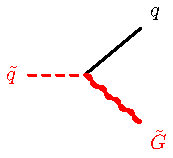
\includegraphics[width=0.3\textwidth]{BeyondSM/Figures/sqqN.eps}
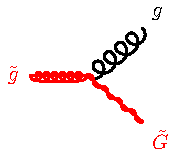
\includegraphics[width=0.3\textwidth]{BeyondSM/Figures/glgN.eps}
}
\mbox{
}
\end{center}
\caption[Feynman diagrams for the squark and gluino decays in GMSB scenarios.]{Leading order Feynman diagrams for the decays of the squark (right) and gluino (left) to a gravitino and a squark or a gluino, respectively, in the GMSB scenario considered.}
\label{fig:DiagramsVertexGravitinoGMSB}
\end{figure}

The $\gravino + \gluino$ production is driven by two competing initial states, i.e. quark-antiquark or gluon-gluon scattering, while the $\gravino + \squark$ can only be produced in quark-gluon collisions due to fermion number conservation.
For the different production processes (see Figure \ref{fig:DiagramsGravitinoGMSB}), the differential cross section,

\begin{figure}[!ht]
\begin{center}
\mbox{
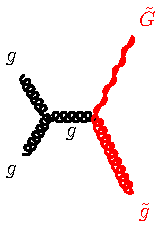
\includegraphics[width=0.3\textwidth]{BeyondSM/Figures/Gravitino_ggg.eps}
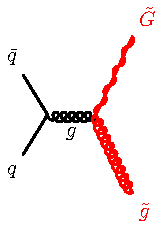
\includegraphics[width=0.3\textwidth]{BeyondSM/Figures/Gravitino_qgq.eps}
}
\newline
\mbox{
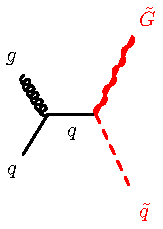
\includegraphics[width=0.3\textwidth]{BeyondSM/Figures/Gravitino_qqg.eps}
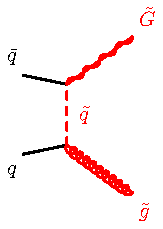
\includegraphics[width=0.3\textwidth]{BeyondSM/Figures/Gravitino_qsqq.eps}
}
\end{center}
\caption{Feynman diagrams for the gravitino production in GMSB scenarios at LO.}
\label{fig:DiagramsGravitinoGMSB}
\end{figure}

\begin{equation}
\frac{d\hat{\sigma}}{dt} = \frac{1}{2s}\frac{1}{8\pi s}|\bar{M}|^2,
\label{eq:SUSYGMSBproductionXSectionGeneral}
\end{equation}

\noindent depends on the Mandelstam variables $s$, $t$, $u$, and the gravitino mass, $m_{3/2}$.
Predictions for the differential cross-sections are computed at LO in pQCD neglecting the gravitino mass everywhere but in the coupling constants:

\begin{equation}
\begin{split}
|\bar{M}|^2_{q\bar{q}\rightarrow \gravino \gluino} &= \frac{g_s^2 C_F}{3 N_C M_P^2 m_{3/2}^2} F_{q\bar{q}\rightarrow \gravino \gluino}(s, t, u, m_{3/2}) \\
|\bar{M}|^2_{gg\rightarrow \gravino \gluino} &= \frac{g_s^2 m_{\gluino}}{6 C_F M_P^2 m_{3/2}^2} F_{gg\rightarrow \gravino \gluino}(s, t, u, m_{3/2}, m_{\gluino}) \\
|\bar{M}|^2_{qg\rightarrow \gravino \gluino} &= \frac{g_s^2}{12 N_C M_P^2 m_{3/2}^2} F_{q/g\rightarrow \gravino \gluino}(s, t, u, m_{\squark}, m_{\gluino}),
\end{split}
\label{eq:SUSYGMSBProductionSpecific}
\end{equation}

\noindent where the functions $F_{q\bar{q}\rightarrow \gravino \gluino}$, $F_{gg\rightarrow \gravino \gluino}$ and $F_{q/g\rightarrow \gravino \gluino}$ are shown in Ref.~\cite{Klasen:2006kb}.
Even though the differential cross section is suppressed by powers of $M_P^2$, there is a dependence $\sim 1/m_{3/2}^2$, and therefore lower bounds on $m_{3/2}$ can be extracted from cross section constraints.


\subsection{Simplified MSSM models}
    \label{subsec:SimplifiedMSSMmodelsTheory}

The MSSM is the minimal supersymmetric extension of the SM. 
It has 124 free input parameters to be tuned, that parametrize the ignorance about how SUSY is broken.
In order to facilitate the exploration of the MSSM phenomena, a variety of simplified models are considered.
Simplified models allow to capture the main features of the sensitivity of the LHC searches to a certain model, without having to explore all the parameter space.
In some cases, the gluino, sbottom and stop quarks are decoupled from the rest of the supersymmetric spectrum.
In this specific simplified model, only light flavor squark-antisquark production is allowed and this process is flavor blind, if the masses are considered degenerate.
In other cases, the opposite holds, thus aiming to study stop and sbottom pair production at colliders.
Other types of simplified models decouple not only the squarks from the third generation particles, but also all the right-handed squarks, thus focusing on final state decays via charginos or neutralinos.

\subsubsection{Direct stop and sbottom production}

At hadron colliders, diagonal pairs of stop and sbottom particles can be produced at lowest order in pQCD in quark-antiquark annihilation and gluon-gluon fusion:

\begin{equation}
\begin{matrix}
q \bar{q} \rightarrow & \stopone \antistopone, & \stoptwo \antistoptwo, & \sbottomone \antisbottomone &\text{  and  } & \sbottomtwo \antisbottomtwo\\
gg        \rightarrow & \stopone \antistopone, & \stoptwo \antistoptwo, & \sbottomone \antisbottomone &\text{  and  } & \sbottomtwo \antisbottomtwo \\
\end{matrix}
\label{eq:DirectStopSbottomProduction}
\end{equation}

The relevant leading order diagrams for these processes are found in Figure~\ref{fig:StopProductionDiagrams}, while a full set of higher-order diagrams for the production of top squarks can be found in Ref.~\cite{Beenakker:1997ut}.
The corresponding leading order cross sections for these partonic subprocesses can be written as:

\begin{figure}[!ht]
\begin{center}
\mbox{
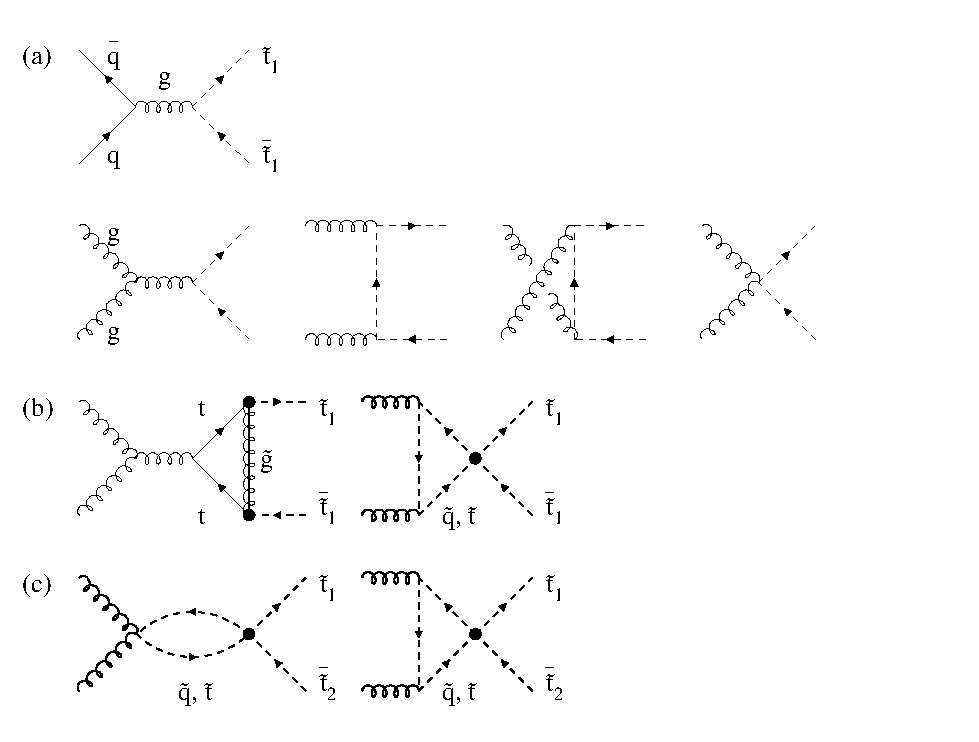
\includegraphics[trim=0.8cm 5.7cm 0cm 0cm, clip=true, width=0.995\textwidth]{BeyondSM/Figures/feyn_fin.eps}
}
\end{center}
\caption[Born diagrams for quark-antiquark annihilation and gluon fusion, leading to pairs of stop particles.]{Born diagrams for quark-antiquark annihilation and gluon fusion, leading to pairs of stop particles~\cite{Beenakker:1997ut}.}
\label{fig:StopProductionDiagrams}
\end{figure}

\begin{equation}
\begin{split}
\sigma_{q\bar{q} \rightarrow \tilde{q}_k\bar{\tilde{q}}_k} &= \frac{\alpha_s^2 \pi}{s} \frac{2}{27} \beta_k^3 \\
\sigma_{gg \rightarrow \tilde{q}_k \bar{\tilde{q}}_k} &= \frac{\alpha_s^2 \pi}{s} \left\{ \beta_k \left( \frac{5}{48} + \frac{31 m_{\tilde{q}_k}^2}{24s}\right) + \left(\frac{2m_{\tilde{q}_k}^2}{3s} + \frac{m_{\tilde{q}_k}^4}{6s^2}\right)\log{\left(\frac{1-\beta_k}{1+\beta_k}\right)} \right\} ,
\end{split}
\label{eq:StopSbottomCrossSection}
\end{equation}

\noindent where $k=1, 2$, $\squark = \stop, \sbottom$ and $\beta_k = \sqrt{1 - 4m_{\tilde{q}_k/s}}$.
Different simplified models are considered involving production of third generation squarks in the analysis presented in this Thesis:

\begin{itemize}
\item{Stop pair production with $\stoptocharm$:} The gluino together with the first and second squark generations are decoupled from the theory.
\item{Stop pair production with $\stopfourbody$:} Same prescription as stop pair production with $\stoptocharm$.
\item{Sbottom pair production with $\sbottomtob$:} Same prescription as stop pair production with $\stoptocharm$.
\end{itemize}

Figure \ref{fig:Diagrams3rdGen} shows the Feynman diagrams for these three processes.

\begin{figure}[!ht]
\begin{center}
\mbox{
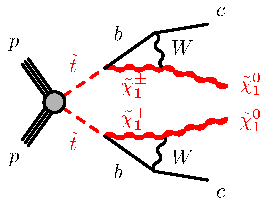
\includegraphics[width=0.3\textwidth]{BeyondSM/Figures/stst-ccN1N1-bWC1loop.eps}
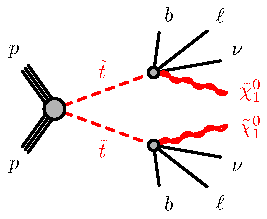
\includegraphics[width=0.3\textwidth]{BeyondSM/Figures/stst-blvblvN1N1-4body.eps}
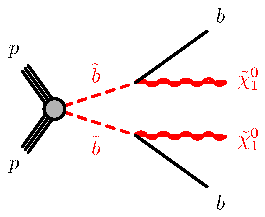
\includegraphics[width=0.3\textwidth]{BeyondSM/Figures/sbsb-bbN1N1.eps}
}
\end{center}
\caption[Feynman diagrams for different stop and sbottom pair production processes.]{Feynman diagrams for the direct stop and sbottom production processes studied. Left: stop pair production, with the stops decaying each to a charm quark and a neutralino. Center: Stop pair production with the stops decaying each to a bottom quark, two fermions and a neutralino. Right: sbottom pair production, each decaying to a bottom quark and a neutralino.}
\label{fig:Diagrams3rdGen}
\end{figure}


\subsubsection{Squark and gluino production}

The hadroproduction of squarks and gluinos at leading order, whose Feynman diagrams and cross section computations are shown in Figure~\ref{fig:SquarkGluinoProductionDiagrams} and in Ref.~\cite{Beenakker:1996ch}, respectively, proceeds through the following partonic interactions:

\begin{figure}[!ht]
\begin{center}
\mbox{
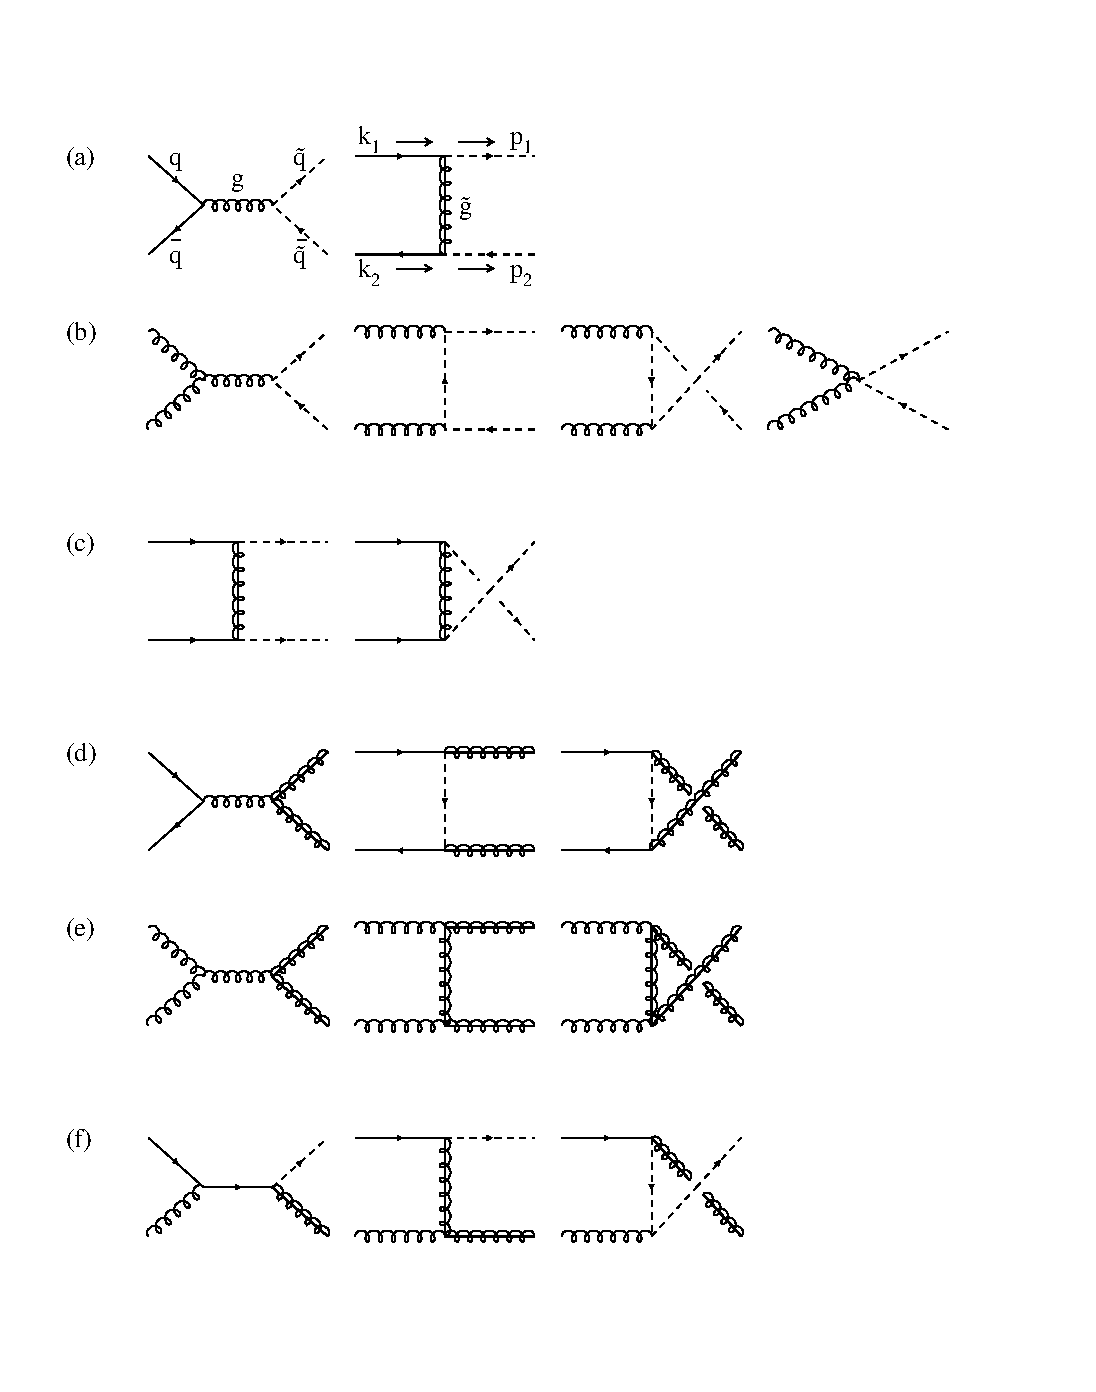
\includegraphics[width=0.995\textwidth]{BeyondSM/Figures/bornfeyn.eps}
}
\end{center}
\caption[Feynman diagrams for the production of squarks and gluinos in lowest order.]{Feynman diagrams for the production of squarks and gluinos in lowest order. The diagrams without and with crossed final-state lines represent $t-$ and $u-$ channel diagrams, respectively. The diagrams in (c) and the last diagram in (d) are a result of the Majorana nature of gluinos. Note that some of the above diagrams contribute only for specific flavors and chiralities of the squarks~\cite{Beenakker:1996ch}.}
\label{fig:SquarkGluinoProductionDiagrams}
\end{figure}

\begin{equation}
\begin{matrix}
\tilde{q} \bar{\tilde{q}} \text{ production: } & q_i + \bar{q}_j &\rightarrow & \tilde{q}_k + \bar{\tilde{q}}_l & \\
& g   + g         &\rightarrow & \tilde{q}_k + \bar{\tilde{q}}_l & \\
\tilde{q} \tilde{q} \text{ production: }       & q_i + q_j       &\rightarrow & \tilde{q}_k + \tilde{q}_l & \text{ and } c.c.\\
\tilde{g} \tilde{g} \text{ production: }       & q_i + \bar{q}_i &\rightarrow & \tilde{g}   + \tilde{g} & \\
& g   + g         &\rightarrow & \tilde{g}   + \tilde{g} & \\
\tilde{q} \tilde{q} \text{ production: }       & q_i + g         &\rightarrow & \tilde{q}_i + \tilde{g} & \text{ and } c.c.
\end{matrix}
\label{eq:DirectSquarkGluinoProduction}
\end{equation}

In this picture, the chiralities of the squarks are not considered explicitly, $\squark = (\squark_L, \squark_R)$, and the indices $i$-$l$ indicate the flavors of the quarks and squarks involved.
In the analysis, only first and second squark generations are considered, degenerated in mass. 

The following simplified models are considered for analysis, while the Feynman diagrams for these processes are shown in Figure~\ref{fig:DiagramsInclusiveProduction}:

\begin{itemize}
\item{Squark pair production with $\squarktoq$: }The third generation squarks and the gluino masses are set to $\unit[5]{TeV}$ and therefore are decoupled from the theory.
\item{Gluino pair production with $\gluinotog$: }Assumed 100\% branching ratio for this decay, with the rest of SUSY particles decoupled, but the neutralino.
\item{Gluino pair production with $\gluinotobb$: }Same prescription as gluino pair production with $\gluinotog$.
\end{itemize}

\begin{figure}[!ht]
\begin{center}
\mbox{
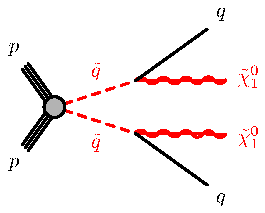
\includegraphics[width=0.3\textwidth]{BeyondSM/Figures/sqsq-qqN1N1.eps}
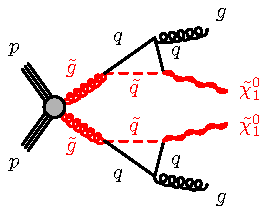
\includegraphics[width=0.3\textwidth]{BeyondSM/Figures/gogo-ggN1N1.eps}
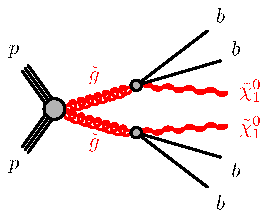
\includegraphics[width=0.3\textwidth]{BeyondSM/Figures/gogo-bbbbN1N1.eps}
}
\end{center}
\caption[Feynman diagrams for different inclusive squark/gluino production processes.]{Feynman diagrams for the inclusive squark/gluino production processes studied. Left: inclusive squark pair production, with the squarks decaying each to a quark and a neutralino. Center: gluino pair production with the gluino decaying each to a gluon and a neutralino. Right: gluino pair production, each decaying to a bottom and antibottom quarks and a neutralino.}
\label{fig:DiagramsInclusiveProduction}
\end{figure}


\subsubsection{Processes involving direct production of charginos or neutralinos}

SUSY electroweak particles are usually produced in the cascade decays.
However, they can also be produced directly in electroweak-driven processes, with much lower cross sections in comparison to SUSY strong production~\cite{Kramer:2012bx, Berggren:2013bua}.
In the analysis presented, two simplified model processes involving electroweakinos (whose Feynman diagrams are shown in Figure~\ref{fig:DiagramsElectroweakProduction}) are studied:

\begin{itemize}
\item{$\squarkneutralino$ production: } First and second squark generations are degenerated in mass, while the third generation squarks and the gluino are decoupled from the theory.
\item{$\charginoneutralino$ and $\charginochargino$ production: } All squarks, sleptons and gluino masses are set to more than $\unit[5]{TeV}$.
\end{itemize}

\begin{figure}[!ht]
\begin{center}
\mbox{
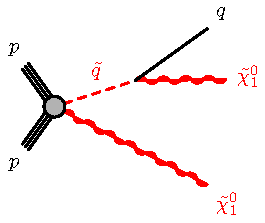
\includegraphics[width=0.3\textwidth]{BeyondSM/Figures/sqN1-qN1N1.eps}
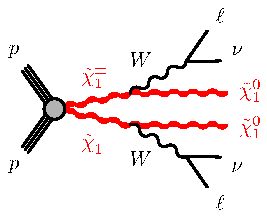
\includegraphics[width=0.3\textwidth]{BeyondSM/Figures/C1C1-llvvN1N1-WW.eps}
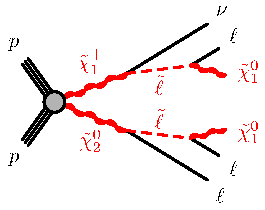
\includegraphics[width=0.3\textwidth]{BeyondSM/Figures/C1N2-lllvN1N1-slsl.eps}
}
\end{center}
\caption[Feynman diagrams for processes involving the direct production of a chargino or a neutralino.]{Feynman diagrams for the electroweak SUSY production processes studied. Left: squark-neutralino production, with the squark decaying to a quark and a neutralino. Center: chargino pair production. Right: Chargino-neutralino production.}
\label{fig:DiagramsElectroweakProduction}
\end{figure}


\section{ADD Large Extra Dimensions}
\label{sec:ADD}

The Arkani-Hamed-Dimopoulos-Dvali \cite{ArkaniHamed:1998rs} (ADD) model of large extra dimensions is a framework which aims to solve the hierarchy problem without relying in supersymmetry.
In particular, this model provides an explanation to the 16 orders of magnitude difference between the electroweak and the Planck scales.
With this objective, $n$ extra spatial compactified dimensions with radius $R$ are added to the $3+1$ space-time dimensions.
Under this assumption, two test masses $m_1$ and $m_2$ placed at a distance $r\muchless R$ would feel a gravitational potential,

\begin{equation}
V(r) \sim \frac{m_1 m_2}{M^{n+2}_D} \frac{1}{r^{n+1}},\;\; (r\muchless R),
\label{eq:ADDPotentialrSmall}
\end{equation}

\noindent where $M_D$ is the Planck scale assuming $n$ extra dimensions.
However, if $r\gg R$,

\begin{equation}
V(r) \sim \frac{m_1 m_2}{M^{n+2}_D} \frac{1}{R^n r},\;\; (r\gg R),
\label{eq:ADDPotentialrBig}
\end{equation}

\noindent which can be related to the Newtonian gravitational potential:

\begin{equation}
V(r) \sim \frac{m_1 m_2}{M^2_P} \frac{1}{r},
\label{eq:ADDPotentialNewton}
\end{equation}

\noindent if the ``effective'' 4-dimensional Planck scale is equivalent to

\begin{equation}
M_P^2 \sim M_D^{2+n} R^n.
\label{eq:ADDPlanckMassEquivalence}
\end{equation}

In the ADD model, the electroweak scale $m_{EW}$ is the only fundamental short scale in nature.
Therefore, if $M_D \sim m_{EW}$, Equation~\ref{eq:ADDPlanckMassEquivalence} leads to:

\begin {equation}
R \sim 10^{\frac{30}{n}-17} \unit[]{cm} \times \left(\frac{\unit[1]{TeV}}{m_{EW}}\right).
\label{eq:ADDRRelation}
\end{equation}

This result points to the fact that $M_D$, the truth strength of the gravitational interaction can be as low as the electroweak scale providing values of $R$ as large as a millimeter.
For $n=1$, $R\sim \unit[10^{13}]{cm}$, which should produce deviations from Newtonian gravity over solar system distances, and therefore is empirically excluded.
For $n=2$, $R\sim \unit[100]{\mu m} - \unit[1]{mm}$, thus leading to deviations in the gravitational predictions that could be proved in the upcoming years\footnote{At present, gravity has been proven at the level of several hundreds of micrometers.}.
Higher $n$ values would lead to lower compactification radii $R$.

In the ADD model, the SM particles can only propagate in a 4-dimensional submanifold, while gravitons, understood as excitations of the $n$-dimensional metric, are the only particles allowed to $4+n$ dimensional bulk.

In terms of 4-dimensional indices, the metric tensor contains spin-2, spin-1 and spin-0 particles, which can be expressed as a tower of Kaluza-Klein modes \cite{KaluzaArticle,KleinArticle}.
The mass of each Kaluza-Klein mode corresponds to the modulus of its momentum in the direction transverse to the 4-dimensional brane.
In fact, the picture of a massless graviton propagating in a $n$-dimensional space or a massive Kaluza-Klein tower of massive gravitons propagating in a 4-dimensional space is completely equivalent.
At low energy and small curvature, the equations of motion of the effective theory reduce to Einstein equation in $n=4+\delta$ dimensions:

\begin{equation}
\mathcal{G}_{AB} \equiv \mathcal{R}_{AB} - \frac{1}{2} g_{AB}\mathcal{R} = - \frac{T_{AB}}{\bar{M}^{2+\delta}_D} \quad\quad A,B = 1,\ldots,n,
\label{eq:ADDEinsteinEquation}
\end{equation}

\noindent where $\bar{M}_D$ is the reduced Planck scale of the $n$-dimensional theory, $M_D = (2\pi)^{\delta/(2+\delta)} \bar{M}_D$.
If the metric $g_{AB}$ is expanded around its Minkowski value $\eta_{AB}$,

\begin{equation}
g_{AB} = \eta_{AB} + 2 \bar{M}_D^{-1-\delta/2}h_{AB},
\label{eq:ADDMinkowskiExpansion}
\end{equation}

\noindent Equation~\ref{eq:ADDEinsteinEquation} can then be rewritten as:

\begin{equation}
\begin{split}
\bar{M}_D^{1+\delta/2} \mathcal{G} &= \Box h_{AB} - \partial_A \partial^C h_{CB} - \partial_B \partial^C h_{CA} + \partial_A \partial_B h^C_C \\
&- \eta_{AB} \Box h_C^C + \eta_{AB}\partial^C \partial^D h_{CD} = - \bar{M}_D^{-1-\delta/2} T_{AB},
\end{split}
\label{eq:ADDEinsteinEquationPowersH}
\end{equation}

\noindent keeping only the first power of $h$.
The previous expression can be derived from the following $n$-dimensional graviton lagrangian:

\begin{equation}
\begin{split}
\lagrangian_{\text{grav}} &= -\frac{1}{2}h^{AB} \Box h_{AB} + \frac{1}{2}h^A_A \Box h^B_B \\
&- h^{AB} \partial_A \partial_B h_C^C + h^{AB} \partial_A \partial_C h_B^C - \frac{1}{\bar{M}_D^{-1-\delta/2}} h^{AB} T_{AB}.
\end{split}
\label{eq:ADDGravitonLagrangian}
\end{equation}

This lagrangian becomes the sum over the Kaluza-Klein modes of:

\begin{equation}
\begin{split}
\lagrangian_{\text{grav}} &= \sum_{\text{all }\vec{n}} -\frac{1}{2} G^{(-\vec{n})\mu\nu} (\Box + m^2)G^{(-\vec{n})}_{\mu\nu} + \frac{1}{2} G^{(-\vec{n})\mu}_{\mu} (\Box + m^2) G^{(-\vec{n})\nu}_{\nu} \\
&- G^{(\vec{n})\mu\nu} \partial_\mu \partial_\nu G^{(\vec{n})\lambda}_{\lambda} + G^{(\vec{n})\mu\nu} \partial_\mu \partial_\lambda G^{(\vec{n})\lambda}_{\nu} - \frac{1}{M_P}G^{(\vec{n})\mu\nu}T_{\mu\nu}, \\
&+ \cdots \\
\end{split}
\label{eq:ADDGravitonLagrangian4D}
\end{equation}

\noindent under the unitary gauge and the parametrization from Reference~\cite{Giudice:1998ck}.
In this equation, the ellipses refer to spin-2, spin-1 and spin-0 particles that are not coupled (or their coupling is very suppressed) to the SM energy-momentum tensor $T_{\mu\nu}$, and therefore play no role in a collider experiment.
The latest term is the graviton interaction lagrangian.
If $T_{\mu\nu}$ is expanded, the Feynman rules for the interactions between gravitons and SM fields can be retrieved.

For not very high $\delta$ (i.e. $\delta \lesssim 6$) the mass difference between the graviton modes is small and the contributions of the different modes can be integrated over the mass.
Under this approximation, the differential cross section for inclusive graviton production is expressed as:

\begin{equation}
\frac{d^2\,\sigma}{dt\; dm} = \frac{2\pi^{\delta/2}}{\Gamma(\delta/2)} \frac{M_P^2}{M_D^{2+\delta}} m^{\delta-1} \frac{d\, \sigma_m}{dt},
\label{eq:ADDCrossSectionmass}
\end{equation}

\noindent where $d\sigma_m/dt$ is the differential cross section for producing a single Kaluza-Klein graviton of mass $m$, found to be:

\begin{equation}
\begin{split}
\frac{d\sigma_m}{dt}(q\bar{q} \rightarrow gG) &= \frac{\alpha_s}{36}\frac{1}{M_P^2 s}F_1(t/s, m^2/s) \\
\frac{d\sigma_m}{dt}(qg \rightarrow qG) &= \frac{\alpha_s}{96}\frac{1}{M_P^2 s}F_2(t/s, m^2/s)\\
\frac{d\sigma_m}{dt}(gg \rightarrow gG) &= \frac{3\alpha_s}{16}\frac{1}{M_P^2 s}F_3(t/s, m^2/s),
\end{split}
\label{eq:ADDCrossSectionIndividualProcess}
\end{equation}

\noindent with the expressions $F_1$, $F_2$ and $F_3$ reported in Reference~\cite{Giudice:1998ck}.
Figure \ref{fig:DiagramsADDProduction} shows the Feynman diagrams for the graviton production at colliders at LO.

The ADD model is an effective theory and therefore, it is only valid up to a given scale, which is assumed to be of the order of $m_{EW}$.
For this reason, the effects of the hypothetical underlying theory are expected to emerge at energy scales close to $M_D$.

\begin{figure}[!ht]
\begin{center}
\mbox{
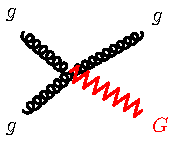
\includegraphics[width=0.3\textwidth]{BeyondSM/Figures/ADD_gggG.eps}
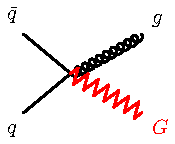
\includegraphics[width=0.3\textwidth]{BeyondSM/Figures/ADD_qqgG.eps}
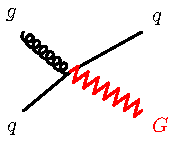
\includegraphics[width=0.3\textwidth]{BeyondSM/Figures/ADD_qgqG.eps}
}
\mbox{
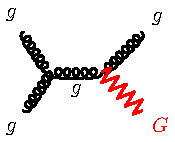
\includegraphics[width=0.3\textwidth]{BeyondSM/Figures/ADD_ggggG.eps}
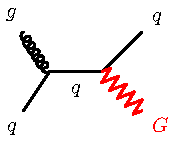
\includegraphics[width=0.3\textwidth]{BeyondSM/Figures/ADD_qgqqG.eps}
}
\end{center}
\caption{Feynman diagrams for the Kaluza-Klein graviton production.}
\label{fig:DiagramsADDProduction}
\end{figure}


\section{Dark Matter and WIMPs}
\label{sec:WIMPs}

The existence of non-luminous matter called ``dark matter'' (DM) in the Universe (see Ref.~\cite{Bertone:2004pz} for a complete review), is inferred from the observation of its gravitational interactions and is well-motivated by experimental observations.
The most convincing evidence for dark matter on galactic scales comes from the observations of the velocity of rotation of stars and gas in spiral galaxies.
If these galaxies were composed only of luminous matter, the circular velocity would be $v(r)\propto 1/\sqrt{r}$ beyond the optical disc.
The fact that $v(r)$ is observed to be approximately constant implies the existence of an halo of DM three to ten times larger than that corresponding to the visible matter, that interacts gravitationally, as shown in Figure \ref{fig:DMProofVelocityStars}.

\begin{figure}[!ht]
\begin{center}
\mbox{
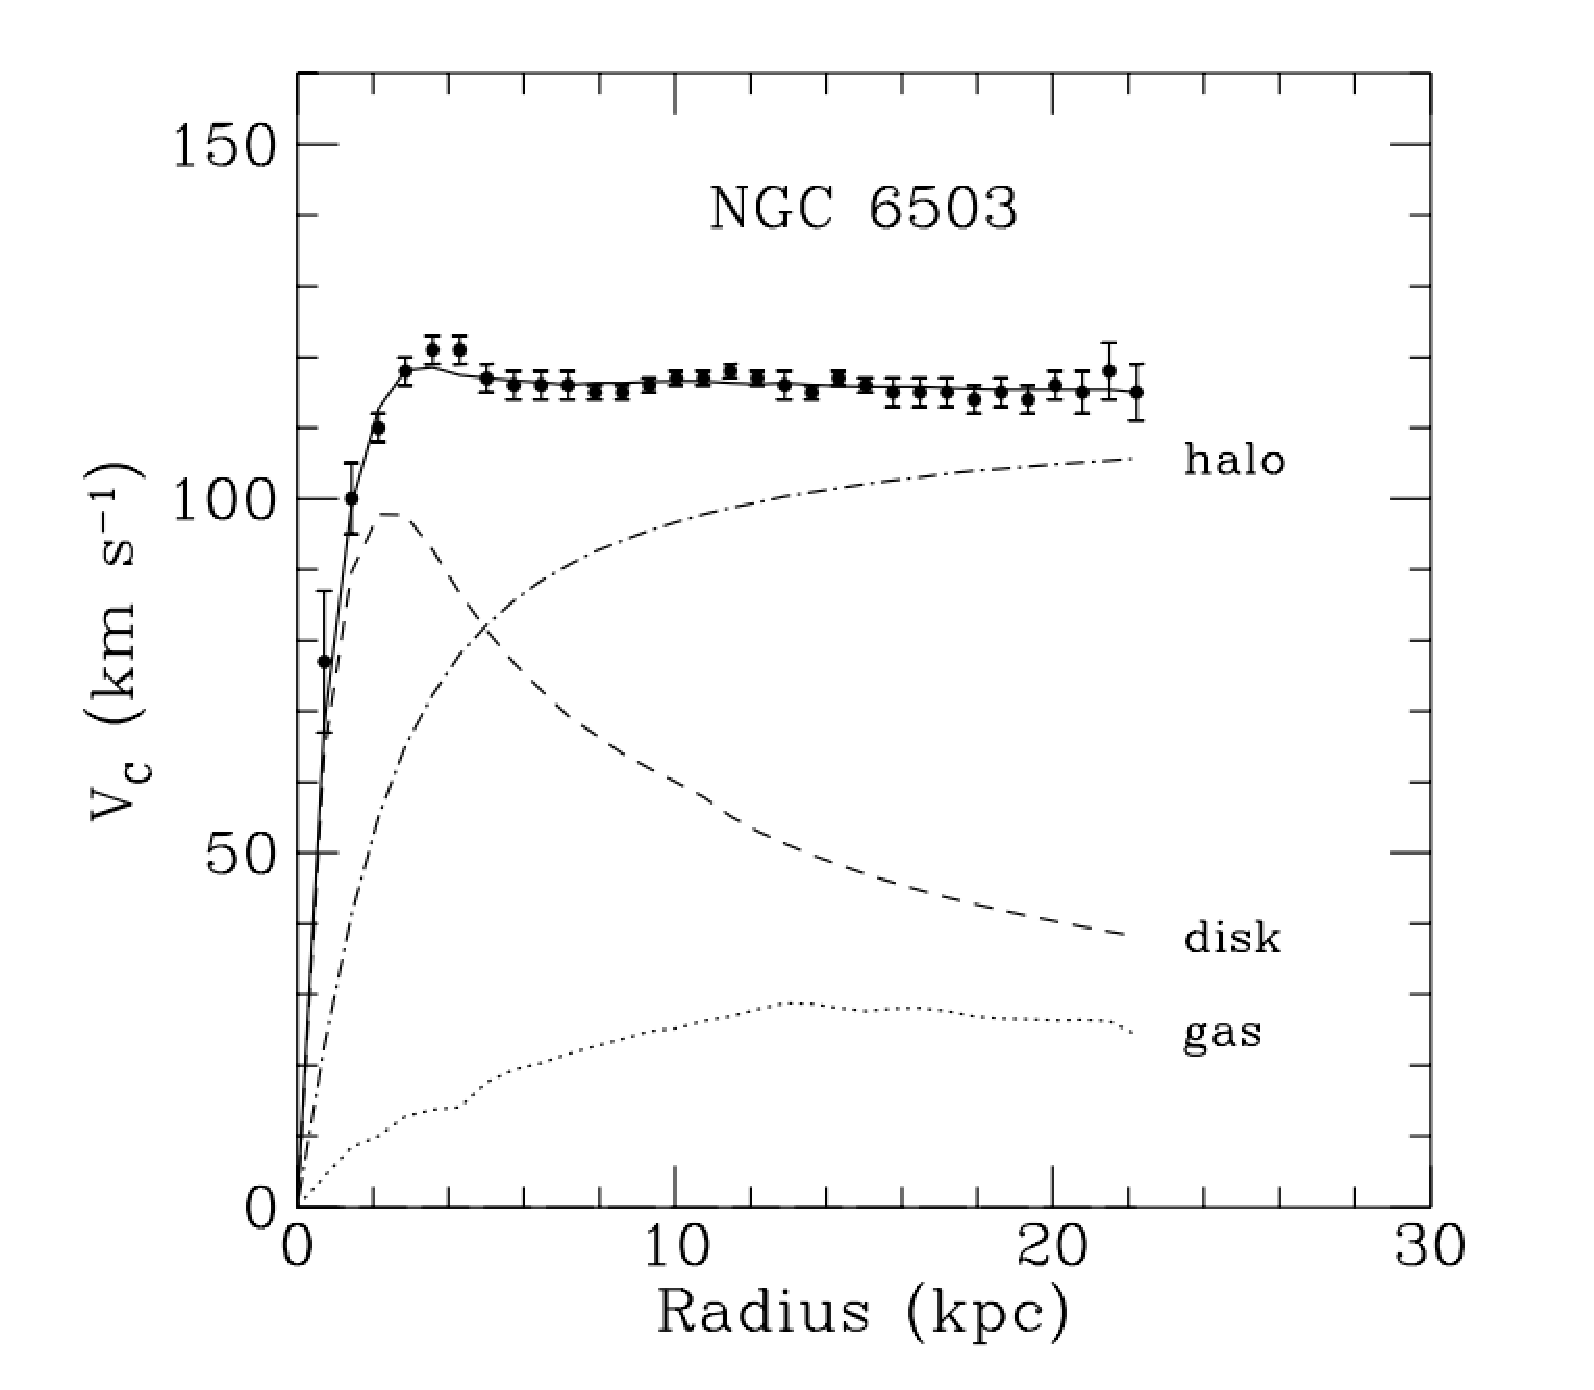
\includegraphics[width=0.495\textwidth]{BeyondSM/Figures/GalaxyVelocityRotation.eps}
}
\end{center}
\caption[Rotational velocity of stars as a function of the radius in the spiral galaxy NGC6503.]{Rotational velocity of stars as a function of the radius in the spiral galaxy NGC6503. The dotted, dashed and dash-dotted lines are the contributions of gas, disk and dark matter, respectively \protect\cite{Begeman:1991iy}.}
\label{fig:DMProofVelocityStars}
\end{figure}

Other evidences for the existence of DM come from a great variety of data, like the strong gravitational lensing.
Weak modulation of strong lensing around individual massive elliptical galaxies \cite{Metcalf:2003sz}, weak gravitational lensing of distant galaxies by foreground structure \cite{Hoekstra:2002nf}, or studies on the velocity dispersions of dwarf spheroidal galaxies \cite{Metcalf:2003sz} also suggest the presence of Dark Matter.

The measurement of the ``cosmic microwave background'' (CMB) also points to the existence of DM. 
The CMB is the thermal radiation background that is measured in the Universe, corresponding to roughly $\unit[2.7]{K}$ of temperature.
It is known to be isotropic at the $10^{-5}$ level.
The CMB is not associated to any specific object, but to the propagation of photons once they were decoupled from matter about $\unit[3.5 \times 10^5]{years}$ after the Big Bang.
A detailed study of the angular correlation in the CMB fluctuations gives information about the geometry of the Universe, about its evolution and its energy-matter content.
Many measurements of the CMB radiation have been performed along the years, the most stringent ones done by the WMAP and the PLANCK experiments~\cite{Larson:2010gs,Ade:2013zuv}.
From these measurements it can be inferred the presence of much larger quantities of dark matter in the early Universe.
A striking coincidence in cosmology is that if DM would annihilate to SM particles with an interaction strength close to that of the weak force, that would result exactly in the decrease of DM density observed between the early and the present Universes.
This coincidence leads to the idea that DM could be composed of Weakly Interacting Massive Particles (WIMPs)~\cite{Zacek:2007mi}.

None of the known SM particles are adequate DM candidates, and for this reason, the existence of a new particles is often hypothesized.
WIMPs, with masses roughly between $\unit[10]{GeV}$ and a few TeV, are one of such class of particle candidates.
They are expected to couple to SM particles through a generic weak interaction, which could be the known weak interaction of the SM or a new type of interaction.
A variety of detection techniques have been developed along the years to search WIMPs, which can be classified depending on the kind of process that they are aimed to observe.
Direct detection experiments aim to observe WIMP-nucleon elastic scattering by measuring the nuclear recoil.
In the last decade, several published results from the direct detection experiments DAMA/LIBRA\cite{Bernabei:2010mq}, CDMS II\cite{Agnese:2013rvf}, CRESST-II\cite{Angloher:2011uu} and CoGent\cite{Aalseth:2010vx} pointed to the existence of light ($\sim\unit[10]{GeV}$) WIMP particles, although these results have been challenged by several other experiments, such as XENON100\cite{Aprile:2012nq}.
Instead, indirect detection experiments search for the SM products from the WIMP-WIMP annihilation.
Finally, collider searches allow the direct production of WIMPs from the annihilation of SM particles.
The sensitivity of collider searches is comparable to the direct and indirect detection searches, especially for low mass WIMPs, since the recoil that the SM particle receives is smaller as the mass of the WIMP decreases.


\subsection{Effective Theory models}

The interaction of WIMPs with SM particles is described as a contact interaction using an effective field theory (EFT) approach, as mediated by a single new heavy particle with mass too large to be produced directly at the LHC.
The use of a contact interaction to produce WIMP pairs via heavy mediators is considered conservative because it rarely overestimates cross sections when applied to a specific BSM scenario.
In this Thesis, WIMPs are assumed to be Dirac-like fermions, and to be odd under the $Z_2$ symmetry, so that each coupling involves an even number of WIMPs.
Different effective operators (described in Table \ref{tab:WIMPsEffectiveOperators}) are considered to describe different bilinear quark couplings to WIMPs.

\begin{table}[tb]
\begin{center}
\begin{tabular}{|cc|cc|}
\hline
\textbf{Name} & \textbf{Operator} & \textbf{Name} & \textbf{Operator} \\
\hline
D1  & $\frac{m_q}{(M^{\ast})^3} \bar{\chi}\chi \bar{q}q$                                         & D2  & $\frac{m_q}{(M^{\ast})^3} \bar{\chi} \gamma^5 \chi \bar{q}q$ \\
D3  & $\frac{m_q}{(M^{\ast})^3} \bar{\chi}\chi \bar{q}\gamma^5 q$                                & D4  & $\frac{m_q}{(M^{\ast})^3} \bar{\chi} \gamma^5 \chi \bar{q} \gamma^5 q$ \\
D5  & $\frac{1}{(M^{\ast})^2} \bar{\chi}\gamma^{\mu} \chi \bar{q} \gamma_{\mu} q$                & D6  & $\frac{1}{(M^{\ast})^2} \bar{\chi}\gamma^{\mu}\gamma^5 \chi \bar{q} \gamma_{\mu} q$ \\
D7  & $\frac{1}{(M^{\ast})^2} \bar{\chi}\gamma^{\mu} \chi \bar{q} \gamma_{\mu} \gamma^5 q$       & D8  & $\frac{1}{(M^{\ast})^2} \bar{\chi}\gamma^{\mu}\gamma^5 \chi \bar{q} \gamma_{\mu} \gamma^5 q$ \\
D9  & $\frac{1}{(M^{\ast})^2} \bar{\chi}\sigma^{\mu\nu} \chi \bar{q} \sigma_{\mu\nu} \gamma^5 q$ & D10 & $\frac{1}{(M^{\ast})^2} \epsilon^{\mu\nu\alpha\beta}\bar{\chi}\sigma_{\mu\nu} \chi \bar{q} \sigma_{\alpha\beta} \gamma^5 q$ \\
D11 & $\frac{1}{(4 M^{\ast})^3} \bar{\chi}\chi \alpha_s (G^a_{\mu\nu})^2$                        & D12 & $\frac{1}{(4 M^{\ast})^3} \bar{\chi} \gamma^5 \chi \alpha_s (G^a_{\mu\nu})^2$ \\
D13 & $\frac{1}{(4 M^{\ast})^3} \bar{\chi}\chi \alpha_s G^a_{\mu\nu} \tilde{G}^{a,\mu\nu}$       & D14 & $\frac{1}{(4 M^{\ast})^3} \bar{\chi} \gamma^5 \chi \alpha_s G^a_{\mu\nu} \tilde{G}^{a,\mu\nu}$ \\
\hline
\end{tabular}
\end{center}
\caption[Effective operators involving couplings between Dirac-like fermion WIMPs and Standard Model quarks or gluons.]{Effective operators involving couplings between Dirac-like fermion WIMPs and Standard Model quarks or gluons~\protect\cite{Goodman:2010ku}.}
\label{tab:WIMPsEffectiveOperators}
\end{table}

In the operator definitions listed in this table, $M^{\ast}$ is the suppression scale of the interaction, after the heavy mediator particle has been integrated.
In the following, only the D5 (vector), D8 (axial-vector) and D9 (tensor) operators from Table~\ref{tab:WIMPsEffectiveOperators} will be considered.

The collider results can also be compared to direct detection experiments, since the WIMP-nucleon cross section is found to be~\cite{Goodman:2010ku}:

\begin{equation}
\begin{split}
\sigma^{D5}_{\chi N} &= 1.38 \times \unit[10^{-37}]{cm^2} \times \left(\frac{\mu_{\chi}}{\unit[1]{GeV}}\right)^2\left(\frac{\unit[300]{GeV}}{M^{\ast}}\right)^4 \\
\sigma^{D8}_{\chi N} &= 4.70 \times \unit[10^{-40}]{cm^2} \times \left(\frac{\mu_{\chi}}{\unit[1]{GeV}}\right)^2\left(\frac{\unit[300]{GeV}}{M^{\ast}}\right)^4 \\
\sigma^{D9}_{\chi N} &= 4.70 \times \unit[10^{-40}]{cm^2} \times \left(\frac{\mu_{\chi}}{\unit[1]{GeV}}\right)^2\left(\frac{\unit[300]{GeV}}{M^{\ast}}\right)^4, \\
\end{split}
\label{eq:WIMP-Nucleon}
\end{equation}

\noindent where $\mu_{\chi}$ is the reduced mass of the WIMP-nucleon system, $\mu_{\chi} = (m_{\chi} \times m_N) / (m_{\chi} + m_N)$.
In direct detection experiments, the typical transferred momentum is of the order of the keV and therefore, the propagator of a mediator with mass $M \gg \unit[1]{keV}$ cannot be resolved, thus making these effective theories suitable for this regime.
However, the LHC center of mass energy of the partons can be up to the TeV scale, and thus targeting a completely different phase space region.
This motivates the need to carefully study the validity of the EFT approach.


\subsection{Simplified models}
    \label{subsubsec:simplifiedModels}

The effective theory models previously introduced, are based on the assumption that the mediator mass is much higher than the scale of the interaction, and for this reason, it cannot be produced directly.
This assumption is not always correct at the LHC, where the momentum transfer can reach the TeV energies.

Instead, simplified models can be used to parametrize the interaction between the quarks and the WIMPs.
These interactions are mediated by a vector particle $Z'$ of a given mass $M_{\text{med}}$, with $\Gamma_{\text{med}}$, and couplings $g_{q}$ and $g_{\chi}$ to the SM particles and WIMPs, respectively.

\cleardoublepage

\chapter{Statistical model}
    \label{chapter:StatisticalModel}

This chapter describes the statistical treatment that is used in the analysis to calculate the normalization of the different background processes, the new physics signal strength, and to estimate the uncertainties.
The general procedure to search for new phenomena is also explained.


\section{Preliminary}
    \label{sec:StatisticsPreliminary}

Some simple case examples are studied first as a way to introduce the complete statistical machinery that will be used in the analysis.

\subsection{One signal region only}

A single region is considered, in which only one signal and one background process are present.
If the presence of any systematic effect is neglected, the probability of finding $n$ data events assuming $B$ expected background events and $S$ expected signal events, the latest normalized with a ``signal strength'', $\mu_s$, follows a Poissonian distribution, and is found to be:

\begin{equation}
P(n | \mu_s S + B) = \frac{(\mu_s S + B)^n}{n!} \exp{\left[-(\mu_s S + B)\right]}.
\label{eq:simplifiedPoisson}
\end{equation}

In the case where $\mu_s=0$, the signal yield is forced to be zero, thus corresponding to a ``background-only'' hypothesis.
On the other hand, $\mu_s=1$ corresponds to the nominal ``signal+background'' hypothesis \cite{Cranmer:2012sba}.
If the probability $P(n | \mu_s S + B)$ is regarded as a function of $\mu_s$, then it is called the likelihood of $\mu_s$, $L(\mu_s)$.
In particular, the maximization of this likelihood function (or equivalently, the minimization of this minus log-likelihood function),

\begin{equation}
-\ln{L(\mu_s)} = -n \ln{(\mu_s S + B)} + (\mu_s S + B) + \ln{n!},
\label{eq:simplifiedLogLikelihood}
\end{equation}

\noindent determines the optimal value for $\mu_s$.


\subsection{Multiple regions, one background process}

The previous example can be extended by considering the background to be corrected by a normalization factor, $\mu_b$, extracted from a calibration measurement in a control region.
Therefore, two regions are considered: a signal region, defined to enhance the signal process, and a control region, orthogonal to the signal region and optimized to enhance the background process.
The probability for finding $\vec{n} = (n_{\text{SR}}, n_{\text{CR}})$ data events assuming $\vec{B} = (B_{\text{SR}}, B_{\text{CR}})$ expected background events and $\vec{S} = (S_{\text{SR}}, S_{\text{CR}})$ expected signal events in both regions is:

\begin{equation}
\begin{split}
P(\vec{n} | \mu_s \vec{S} + \mu_b\vec{B}) &= \frac{(\mu_s S_{\text{SR}} + \mu_b B_{\text{SR}})^{n_{\text{SR}}}}{n_{\text{SR}}!} \exp{\left[-(\mu_s S_{\text{SR}} + \mu_b B_{\text{SR}})\right]} \\
& \times \frac{(\mu_s S_{\text{CR}} + \mu_b B_{\text{CR}})^{n_{\text{CR}}}}{n_{\text{CR}}!} \exp{\left[-(\mu_s S_{\text{CR}} + \mu_b B_{\text{CR}})\right]} ,
\end{split}
\label{eq:simplifiedPoissonControlRegion}
\end{equation}

\noindent where $\mu_s$ and $\mu_b$ are the scale factors for the signal and background processes respectively.
From this probability, the following minus log-likelihood function is derived:

\begin{equation}
\begin{split}
-\ln{L(\mu_s, \mu_b)} =& -n_{\text{SR}} \ln{(\mu_s S_{\text{SR}} + \mu_b B_{\text{SR}})} + (\mu_s S_{\text{SR}} + \mu_b B_{\text{SR}}) \\
                       & -n_{\text{CR}} \ln{(\mu_s S_{\text{CR}} + \mu_b B_{\text{CR}})} + (\mu_s S_{\text{CR}} + \mu_b B_{\text{CR}}) \\
                       & + \ln{n_{\text{SR}}!} + \ln{n_{\text{CR}}!}.
\end{split}
\label{eq:simplifiedLogLikelihoodControlRegion}
\end{equation}

The minimization of $-\ln{L(\mu_s, \mu_b)}$ leads to a system of equations from which the two normalization factors, $\mu_s$ and $\mu_b$ can be computed.


\subsection{Multiple regions, several background processes}
    \label{subsec:StatisticsMultipleRegionsNoSystematics}

The example from the previous subsection can be generalized to having more than one background, normalized with more than one normalization factor.
As a simplification, the signal yield in all the control regions will be considered negligible, $\vec{S} = (S_{\text{SR}}, 0, \ldots)$.
Then, the probability for finding $\vec{n} = (n_\text{SR}, n_\text{CR1}, \ldots)$ data events assuming $\mu_s \cdot \vec{S} + \vec{\mu_b}\cdot \hat{B}$ expected events in the different regions, is found to be:

\begin{equation}
\begin{split}
P(\vec{n} | \mu_s \cdot \vec{S} + \vec{\mu_b}\cdot \hat{B}) &= \frac{(\mu_s S_{\text{SR}} + \sum_{b}^{\text{bkg}}{\mu_{b} B_{{\text{SR}}b}})^{n_{\text{SR}}}}{n_{{\text{SR}}}!} \exp{\left[-(\mu_s S_{{\text{SR}}} + \sum_{b}^{\text{bkg}}{\mu_{b} B_{{\text{SR}}b}})\right]} \\
& \times \prod_{i}^{\text{control}}{ \frac{\left(\sum_{b}^{\text{bkg}}{\mu_{b} B_{ib}}\right)^{n_{i}}}{n_{i}!}} \exp{\left[-\sum_{b}^{\text{bkg}}\mu_{b} B_{ib}\right] }.
\end{split}
\label{eq:simplifiedPoissonSeveralBkg}
\end{equation}

From the previous equation, the likelihood function of $\vec{\mu} = (\mu_s, \mu_{b_1}, \ldots)$ is determined:

\begin{equation}
L(\vec{\mu}) = 
 \prod_{c \in \text{regions}}{\frac{[\nu_c(\vec{\mu})]^{n_c}}{n_c!}e^{-\nu_c(\vec{\mu})}},
\label{eq:generalLikelihoodNoSystematics}
\end{equation}

\noindent where $n_c$ are the number of observed events in the region $c$, and

\begin{equation}
\nu_c = \mu_s S_c + \sum_{j}^{\text{bkg}}{\mu_{b,j}B_{c,j}} = \sum_{s}^{\text{samples}}{\mu_s \nu_{cs}^0},
\label{eq:definitionNuSimple}
\end{equation}

\noindent being $\nu_{cs}^0$ the nominal number of events for the process $s$, in the signal or control region $c$.
Equation~\ref{eq:generalLikelihoodNoSystematics} provides a general likelihood function for a model in which several processes normalized with different normalization factors are measured in different regions, ignoring the effect of any systematic uncertainty.


\subsection{Parametrization of the systematic uncertainties}
    \label{subsec:StatisticsSystematicSimplified}

The expected number of events for a process $s$, in a given region, $c$, can be written as $\eta_{cs} \nu_{cs}^0$, being $\nu_{cs}^0$ the expected nominal yield.
The factor $\eta_{cs}$ is the the relative variation with respect to the nominal expectation due to any systematic effect, and can be regarded as a function of a \emph{nuisance parameter}, $\alpha_p$, which parametrizes the ``number of standard deviations''.

As detailed in Ref.~\cite{Cranmer:2012sba}, different parametrization functions for $\eta_{cs}(\alpha_p)$ can be used, providing that $\eta_{cs}(0)=1$ (by definition, a variation of zero standard deviations must return the nominal yield), and $\eta_{cs}(\pm 1)$ returns exactly the $\pm 1$ standard deviation effect of the systematic uncertainty under study, determined with an auxiliary measurement.

In this example, the nuisance parameter $\alpha_p$ is considered normally distributed according to the probability density function:

\begin{equation}
P(a_p | \alpha_p, \sigma_p) = \frac{1}{\sqrt{2\pi\sigma_p^2}} \exp{\left(-\frac{(a_p - \alpha_p)^2}{2\sigma_p^2}\right)},
\label{eq:simplifiedAlphaParametersPDF}
\end{equation}

\noindent  where $a_p$ is the central value of the auxiliary measurement around which the $\alpha_p$ with standard deviation $\sigma_p$ can be varied when maximizing the likelihood.
The auxiliary measurement $a_p$ and the standard deviation of the gaussian, $\sigma_p$, are typically fixed to 0 and 1, respectively.

The introduction of systematic uncertainties in the analysis implies that the likelihood from Equation~\ref{eq:generalLikelihoodNoSystematics} needs to be multiplied by the PDF from Equation~\ref{eq:simplifiedAlphaParametersPDF}.
This introduces a dependence on $\alpha$ in the sample yields, $\nu_{cs}$.


\section{Complete statistical treatment}
    \label{sec:StatisticalTreatment}

The complete statistical treatment of the analysis is based on the profile likelihood method, which results from the combination and generalization of the simplified examples discussed above.
This method allows to determine the normalization factors to be applied to estimate the different processes as well as the systematic variations and the correlations among them.
As in the previous examples, no shape information is used in the analysis presented in this Thesis: the distributions in the signal and control regions consist of just one single bin.

\subsection{Parametrization of the model}
    \label{subsec:ParametrizationModel}

The signal and the backgrounds in the different region definitions, as well as the systematic uncertainties under consideration are parametrized by the likelihood function (see Equations~\ref{eq:generalLikelihoodNoSystematics} and \ref{eq:simplifiedAlphaParametersPDF}, in the previous section):

\begin{equation}
L(\vec{\mu}, \vec{\alpha}) = 
 \prod_{c \in \text{regions}}{\frac{[\nu_c(\vec{\mu}, \vec{\alpha})]^{n_c}}{n_c!}e^{-\nu_c(\vec{\mu}, \vec{\alpha})}}
 \prod_{p\in\text{params}}{P_p(\alpha_p)},
\label{eq:PdfFit}
\end{equation}

\noindent where $n_c$ are the number of events measured in each region, $\vec{\mu}$ is the set of normalization factors used to normalize the different background and signal processes, and $\vec{\alpha}$ is a set of nuisance parameters that parametrize the different systematic uncertainties.
Furthermore, $\nu_c$ are the number of events expected in each region, in particular (see Equation~\ref{eq:definitionNuSimple}):

\begin{equation}
\nu_c(\vec{\mu}, \vec{\alpha}) = \sum_{s\in\text{samples}}{\mu_s(\vec{\alpha})\;\eta_{cs}(\vec{\alpha})\;\nu^0_{cs}},
\label{eq:nuInPdfFit}
\end{equation}

\noindent where $\nu^0_{cs}$ is the expected nominal number of events and $\eta_{cs}$ is the parametrized normalization uncertainty, that depend on the nuisance parameters $\vec{\alpha}$.
Finally, $P_p$ is a constraining term, that describes an auxiliary measurement to used constrain the nuisance parameter $\alpha_p$.
In the present analysis, the constraining term is assumed to be a gaussian, except for the nuisance parameters dedicated to the statistical uncertainties, which are poissonian distributed.

The maximization of this function allows to calculate the normalization factors and nuisance parameters used to estimate the yield of each process and the level of systematics in the different regions.
In the analysis, three fit configurations will be used for different purposes \cite{Baak:2014wma}:

\paragraph{Background-only fit:}Only the control regions are used to constrain the fit parameters. 
Any potential signal contribution is neglected everywhere ($\mu_\text{signal} = 0$).
This fit is used to extract the normalization factors of the background processes and their systematic uncertainties.

\paragraph{Model independent signal fit:}Both control and signal regions are used in the fit. 
The signal is independently considered in each signal region but neglected in the control regions.
This background prediction is conservative since any signal contribution in the control regions is attributed to background and thus results in a possible overestimation of the background in the signal regions. 
In this analysis this contribution is negligible due to the requirement of leptons in the control regions.
This fit configuration is used to extract the 95\%~CL model independent upper limits on the visible cross section.

\paragraph{Model dependent signal fit:}Both control and signal regions are used in the fit. 
The signal contribution is taken into account as predicted by the tested model in all the regions.
The model dependent signal fit configuration is used to interpret the results of this analysis in terms of the different new physics models that are studied.


\section{Statistical tests}
    \label{subsec:StatisticalTests}

This section describes the general procedure used to search for a new phenomena in the context of a frequentist statistical test.
If the purpose of the analysis is to discover a new signal process, the null hypothesis, $H_0$, is defined as describing the known SM processes, to be tested against $H_1$, which includes both background as well as the signal model.
Instead, if the purpose of the analysis is to set limits on a signal process, the model with signal plus background plays the role of $H_0$, tested against the background-only hypothesis, $H_1$.
In the outcome of such search, the level of agreement of the observed data with a given hypothesis $H$ is quantified by computing the probability, under the assumption of $H$, of finding data with equal or less incompatibility with the prediction of $H$.

According to Equation \ref{eq:nuInPdfFit}, each process is multiplied by a normalization factor, $\mu$.
A background-only hypothesis is constructed by fixing $\mu_\text{signal}=0$, while a signal+background hypothesis will be defined as having $\mu_\text{signal}\gt0$.
To test an hypothesized value of $\mu$, the profile likelihood can be defined as the ratio:

\begin{equation}
\lambda(\mu) = \frac{L(\mu, \vec{\hat{\hat{\theta}}})}{L(\hat{\mu}, \vec{\hat{\theta}})},
\label{eq:profileLikelihood}
\end{equation}

\noindent where $\mu$ here is the shortcut for $\mu_\text{signal}$ and $\vec{\theta}\supset\{\mu_{\text{no signal}}, \vec{\alpha}\}$.
$\vec{\hat{\hat{\theta}}}$ in the numerator denotes the value of $\vec{\theta}$ that maximizes $L$ for the specified $\mu$ (it is a conditional maximum likelihood estimator of $\theta$, and therefore a function of $\mu$).
The denominator is the maximized (unconditional) likelihood function.
Based on Equation~\ref{eq:profileLikelihood}, the test statistic $q_\mu$ is defined as:

\begin{equation}
q_\mu = -2\ln{\lambda(\mu)}.
\label{eq:testStatistic}
\end{equation}

Higher values of $q_\mu$ correspond to increasing compatibility between the data and $\mu$.
The $p$-value, defined to quantify the level of agreement between the data and the different hypotheses, is defined as:

\begin{equation}
p_\mu = \int_{q_{\mu,\;\text{obs}}}^{\infty}{f(q_\mu|\mu')\;dq_\mu},
\label{eq:pValueDefinition}
\end{equation}

\noindent where $f(q_\mu|\mu')$ denotes the PDF of $q_\mu$ under the assumption of the signal strength $\mu'$.
The estimations of $f(q_\mu|\mu')$ can be done with pseudo-experiments using Monte Carlo methods (Toy MC).
These methods are computationally heavy, especially when upper limits are calculated.
For this reason, an approximation valid in the large sample limit is normally used to describe the profile likelihood ratio instead (asymptotic approximation).

In the large sample limit, where the asymptotic approximation becomes exact, the PDF of $q_\mu$ assuming that the fitted strength parameter $\hat{\mu}$ follows a gaussian of mean $\mu'$ and standard deviation $\sigma$ is found to be \cite{Cowan:2010js}:

\begin{equation}
\begin{split}
&f(q_\mu|\mu')  = 
\frac{1}{2\sqrt{q_\mu}}\frac{1}{\sqrt{2\pi}} \times \\
& \left[\exp{\left(-\frac{1}{2}\left(\sqrt{q_\mu}+\frac{\mu-\mu'}{\sigma}\right)^2 \right)} 
+ \exp{\left(-\frac{1}{2}\left(\sqrt{q_\mu}-\frac{\mu-\mu'}{\sigma}\right)^2 \right)} \right].
\end{split}
\label{eq:pdfTestStatistic}
\end{equation}

Figure~\ref{fig:pdfTestStatisticExample} illustrates the previous equation, for the particular case of $q_{\mu=1}$ under a signal plus background and a background-only hypotheses, namely $\mu'=1$ and $\mu'=0$, respectively.
In this example, the requirement that the $p$-value computed from the $f(q_{\mu=1}|1)$ PDF is smaller than 0.05, would be enough to exclude the signal model at 95\% confidence level (CL).
However, the PDFs for both hypotheses could be similar.
These are cases in which the analysis has very low sensitivity and the effect produced by a statistical fluctuation could allow the exclusion of both the null (in this case, the signal plus background) and the alternate (background-only) hypotheses at the same time.
In an attempt to address this spurious exclusion, the $CL_s$ method is developed.
The $CL_s$ solution bases the test not only on the rejection of the null hypothesis but rather in the $p$-value of the null hypothesis divided by one minus the p-value of the alternate hypothesis.
Following the same illustrative example from Figure~\ref{fig:pdfTestStatisticExample}, in which the existence of a given signal model is tested, the $CL_{s+b}$, $CL_{b}$ and $CL_{s}$ can be defined, respectively, as:

\begin{equation}
\begin{split}
CL_{s+b} = p_{s+b} \\
CL_{b} = 1-p_{b} \\
CL_{s} = \frac{CL_{s+b}}{CL_{b}}.
\end{split}
\label{eq:CLsDefinition}
\end{equation}

\begin{figure}[!t]
  \begin{center}
    \mbox{
      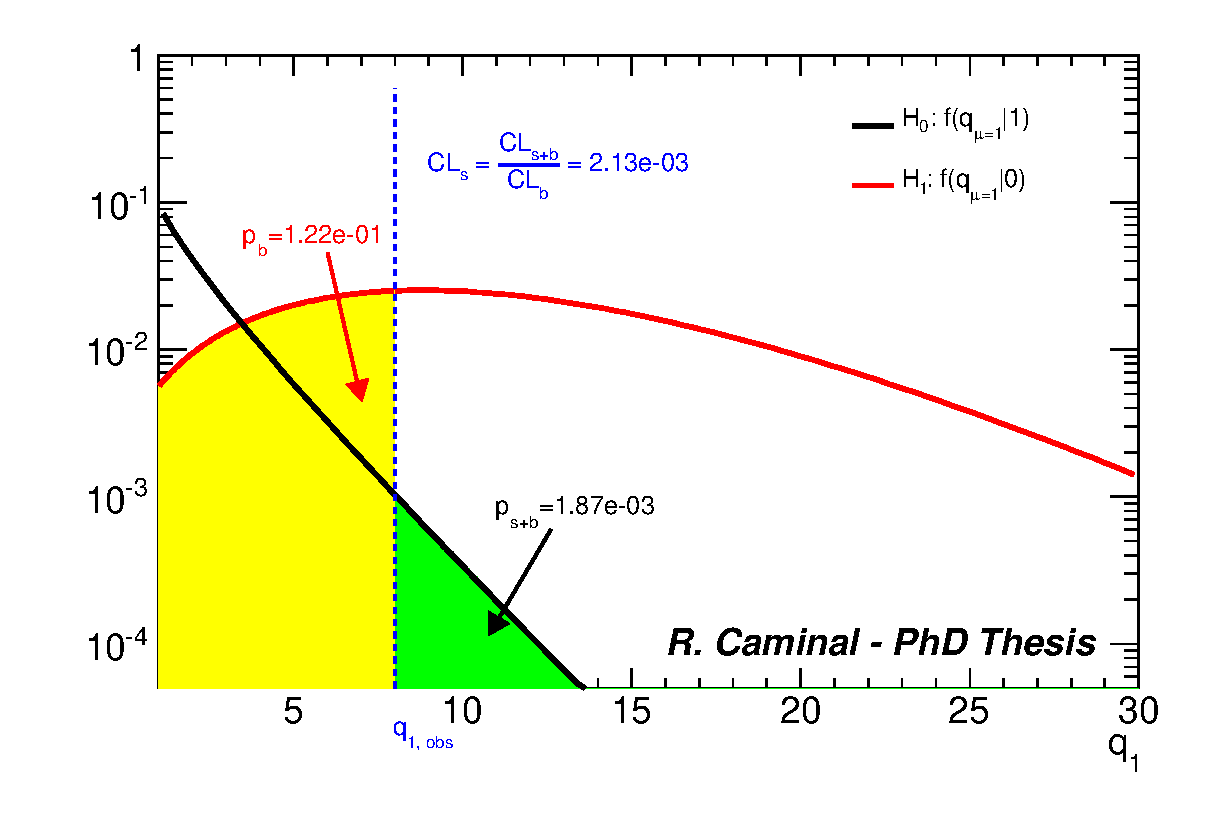
\includegraphics[width=0.75\textwidth]{MonojetAnalysis/Figures/pdfTestHypothesisExample.eps}
    }
  \end{center}
  \caption[Illustration of the PDF of $q_{\mu}$ under the signal plus background and background-only hypotheses.]{Illustration of the PDF of $q_{\mu=1}$ under two different hypothesis: signal plus background (null, $\mu=1$) and background-only (alternative, $\mu=0$). The $CL_{s+b}$, $CL_b$ and $CL_s$ are also shown for this particular example.}
  \label{fig:pdfTestStatisticExample}
\end{figure}

In the work presented in this thesis, the $CL_s$ is calculated for each signal model under evaluation.
The models for which $CL_s < 0.05$, are excluded at 95\% CL.
With the $CL_s$ method, $CL_s \approx CL_{s+b}$ in the cases where the analysis is sensitive to the signal process under study.
Instead, in the cases where the analysis is insensitive, $CL_b$ is be small, thus increasing the value of $CL_s$ and therefore avoiding the exclusion of the signal model.

\cleardoublepage

\chapter{The ATLAS detector at the LHC}
    \label{chapter:ATLASDetector}

The analysis described in this Thesis is performed using proton-proton collision data produced in the Large Hadron Collider and detected and reconstructed by the ATLAS detector.
This chapter introduces the CERN's accelerator complex and describes the main aspects of the ATLAS detector at the LHC. 

\section{The Large Hadron Collider}
    \label{sec:LHC}

The Large Hadron Collider (LHC)~\cite{Evans:2008zzb} is a circular superconducting particle accelerator installed in a $\unit[27]{km}$ long underground tunnel (between 45~m and 170~m below the surface) that used to host the Large Electron-Positron (LEP) collider.
On the accelerator ring four detectors (ALICE~\cite{Aamodt:2008zz}, ATLAS~\cite{Aad:2008zzm}, CMS~\cite{Chatrchyan:2008aa} and LHCb~\cite{Alves:2008zz}) have been built around four different interaction points to reconstruct and study the collisions delivered by the LHC. 
The LHC is designed to collide protons at a center of mass energy of $\sqrt{s} = \unit[14]{\TeV}$. 

Since 2010, the LHC has delivered proton-proton ($\pp$) collisions at center of mass energies of \unit[7]{\TeV} and \unit[8]{\TeV} (in 2011 and 2012, respectively), about half of its nominal energy. The LHC has produced also lead ion (Pb-Pb) collisions with a per-nucleon center of mass energy $\sqrt{s_{NN}} = \unit[2.76]{\TeV}$ and proton-ion (p-Pb) collisions with $\sqrt{s_{NN}} = \unit[5.02]{\TeV}$.

\section{The ATLAS experiment}
    \label{sec:ATLASexperiment}

ATLAS (A Toroidal LHC ApparatuS) is one of the two general-purpose experiments at the LHC. 
It is cylindrically shaped and it measures \unit[46]{m} long, \unit[25]{m} wide and weights \unit[7000]{t}.
ATLAS is specifically designed to reconstruct and identify the main proton-proton collision products (electrons, muons, taus, photons, jets and missing transverse energy). 

ATLAS consists of an assembly of several sub-detectors arranged concentrically around the beam axis, each of them playing a specific role (see Figure~\ref{fig:ATLASsketch}). 
The Inner Detector (ID) is the innermost sub-detector and is able to measure the track properties of the charged particles. 
Surrounding the ID there is the electromagnetic calorimeter, where the electrons and photons are expected to release their energy. 
The third sub-detector is the hadronic calorimeter, where most of the hadronic shower is contained.
Finally, the outermost layer is the muon spectrometer (MS) which measures the properties of the muons.
Furthermore, ATLAS uses a solenoidal magnetic field for bending the particle trajectories in the inner detector and a toroidal magnetic field for the muon spectrometer.

\begin{figure}[!ht]
  \begin{center}
    \mbox{
      \includegraphics[width=0.995\textwidth]{ATLASdetector/Figures/ATLAS_Detector.eps}
    }
  \end{center}
  \caption[View of the full ATLAS detector.]{View of the full ATLAS detector \protect\cite{Evans:2008zzb}.}
  \label{fig:ATLASsketch}
\end{figure}

The ATLAS reference system is a cartesian right-handed coordinate system with origin at the nominal interaction point (IP) in the center of the detector. 
The positive $z$-axis is defined along the anti-clockwise beam direction.
The $x$-axis points from the IP to the center of the LHC ring, and the $y$-axis points upwards. 
The azimutal angle $\phi$ is measured around the beam axis, and the polar angle $\theta$ is measured with respect to the $z$-axis.
The pseudo-rapidity is defined as:

\begin{equation}
  \eta = -\ln{\left(\tan{\frac{\theta}{2}}\right)}.
  \label{eq:pseudorapidity}
\end{equation}

The transverse momentum, $\pt$, the transverse energy, $\et$, and the missing transverse energy, $\met$, are defined in the $x$-$y$ plane.
The angular distance $\Delta R$ is defined as:

\begin{equation}
  \Delta R = \sqrt{(\Delta\eta)^2 + (\Delta\phi)^2}, 
  \label{eq:deltaR}
\end{equation}

\noindent where $\Delta\eta$ is the difference in $\eta$ and $\Delta\phi$ is the difference in $\phi$.
The former is invariant under longitudinal Lorentz boosts for massless objects, while the latter is always invariant under longitudinal Lorentz transformations.

A more accurate description of the ATLAS sub-detectors can be found in the following sections, while a summary of their $|\eta|$ coverage and expected $\pt$ and $\et$ resolution can be found in Table \ref{tab:subdetectorResolution}.

\begin{table}[!ht]
  \begin{center}
    \begin{small}
      \setlength{\tabcolsep}{0.0pc}
      \begin{tabular*}{\textwidth}{@{\extracolsep{\fill}}cccc}
        \noalign{\smallskip}\hline\hline\noalign{\smallskip}
         Detector      & \multirow{2}{*}{required resolution} & \multicolumn{2}{c}{$|\eta|$ coverage} \\
         component     &                                      & Measurement       & Trigger \\
        \noalign{\smallskip}\hline\hline\noalign{\smallskip}
        Tracking (ID)  & $\sigma_{\pt}/\pt = 0.05\%$ $\pt\oplus1\%$ & $<2.5$ & \\
        \noalign{\smallskip}\hline\noalign{\smallskip}
        EM calorimetry  & $\sigma_{E}/E = 10\% / \sqrt{E}\oplus0.7\%$ & $<3.2$ & $<2.5$ \\
        \noalign{\smallskip}\hline\noalign{\smallskip}
        Hadronic  &  & & \\
        calorimetry  &  & & \\
        barrel and end-cap  & $\sigma_{E}/E = 50\% / \sqrt{E}\oplus3\%$ & $<3.2$ & $<3.2$ \\
        forward  & $\sigma_{E}/E = 100\% / \sqrt{E}\oplus10\%$ & $3.1-4.9$ & $3.1-4.9$ \\
        \noalign{\smallskip}\hline\noalign{\smallskip}
        Muon  & \multirow{2}{*}{$\sigma_{\pt}/\pt = 100\% \text{ at } \pt = \unit[1]{\TeV}$} & \multirow{2}{*}{$<2.7$} & \multirow{2}{*}{$<2.4$} \\
        spectrometer & & & \\
        \noalign{\smallskip}\hline\hline\noalign{\smallskip}
      \end{tabular*}
    \end{small}
  \end{center}
  \caption[Summary of ATLAS sub-detectors $|\eta|$ coverage and expected resolution.]{Summary of the ATLAS sub-detectors $|\eta|$ coverage, and the expected energy and $\pt$ resolution~\cite{Evans:2008zzb}.}
  \label{tab:subdetectorResolution}
\end{table}


\subsection{Inner detector}
    \label{subsec:InnerDetector}

The Inner Detector (ID) is the innermost part of ATLAS and it is used to reconstruct tracks and decay vertices.
It is immersed in a \unit[2]{T} solenoidal magnetic field.
Fast response electronics, good radiation resistance and 87 million readout channels allow high precision track measurements in the very large density of tracks in the events produced by the LHC.
The ID is $\unit[6.2]{m}$ long and $\unit[2.1]{m}$ in diameter, covering a range $|\eta|<2.5$. 
It is divided in three different concentric sub-detectors, named (increasing in distance with respect to the IP) pixel, semi-conductor tracker (SCT) and transition radiation tracker (TRT). Figure~\ref{fig:InnerDetector} shows a cut-away view of the ATLAS ID.
Using the combined information from the three sub-detectors, the transverse momentum resolution measured with the cosmic muons \cite{Aad:2010mr} is:

\begin{equation}
  \frac{\sigma_{\pt}}{\pt} = P_{1} \oplus P_{2} \times \pt, 
  \label{eq:IDresolution}
\end{equation}

\noindent where $P_{1} = \unit[1.6 \pm 0.1]{\%}$ and $P_{2} = \unit[(53 \pm 2)\times 10^{-5}]{\GeV^{-1}}$. This translates in a resolution of $1.6\%$ for tracks with $\pt\sim \unit[1]{\GeV}$ and of about 50\% for $\pt\sim \unit[1]{\TeV}$.

\begin{figure}[!ht]
  \begin{center}
    \mbox{
      \includegraphics[width=0.995\textwidth]{ATLASdetector/Figures/InnerDetector.eps}
    }
  \end{center}
  \caption[Cut-away view of the ATLAS Inner Detector.]{Cut-away view of the ATLAS Inner Detector \protect\cite{Evans:2008zzb}.}
  \label{fig:InnerDetector}
\end{figure}


\subsubsection{Pixel}
    \label{subsubsec:Pixel}

The pixel detector is the innermost part of the ID and measures charged particles using radiation hard silicon sensors (pixels).
With 80.4 million readout channels, it mainly contributes to precision vertex reconstruction.
A pixel sensor has a minimum size of $\unit[50 \times 400]{\mu m^2}$, and altogether provide a resolution of $\unit[10]{\mu m}$ in the $R-\phi$ plane.

\subsubsection{Semi-Conductor Tracker}
    \label{subsubsec:SCT}

The Semiconductor Tracker (SCT) is the middle part of the ID and is a silicon microstrip detector. It is composed of layers of stereo strips. Eight strip layers are crossed by each track and, since the position is determined from hits in overlapping strips, four space-points per track are usually available.
The mean pitch of each strip is $\unit[80]{\mu m}$ and it makes use of 6.3 millions readout channels.
The SCT mainly contributes to momentum reconstruction, and provides a resolution of $\unit[17]{\mu m}$ in the $R-\phi$ plane.

\subsubsection{Transition Radiation Tracker}
    \label{subsubsec:TRT}

The Transition Radiation Tracker (TRT) is the outermost part of the ID. 
It consists of 4 millimeter diameter gaseous straw tubes interleaved with transition radiation material, enabling tracking for $|\eta|<2$.
Each straw is made of Kapton with a conducting coating.
It acts as a cathode and is kept at high voltage of negative polarity.
In the center of the straw there is a $\unit[30]{\mu m}$ diameter gold-plated tungsten sense wire.
The TRT is only segmented in $R-\phi$, and it provides a resolution of $\unit[130]{\mu m}$ per straw.
It provides about 35 hits per track, and has 351,000 readout channels.
This sub-detector mainly contributes to electron identification \cite{Aad:2011mk}.


\subsection{Calorimeters}
    \label{subsec:Calorimeters}

The ATLAS calorimeters are surrounding the Inner Detector, and they cover the full $\phi$ space and the range $|\eta|<4.9$, extending radially $\unit[4.25]{m}$. 
Figure~\ref{fig:CalorimetersSchema} shows a schematic view of the ATLAS calorimeters system.
In total, the calorimeter systems have 187,648 cells and 375,000 readout channels, and can be classified in electromagnetic, suited to precisely measure electrons and photons; and hadronic, focussed in collecting the energy from the hadrons. 
The EM calorimeter extends along the $\eta$ region covered also by the ID and its fine granularity allows for a precise measurement of the electron and photon showers.
In the rest of the calorimeter, the granularity is bigger, but sufficient for jet reconstruction and $\met$ measurements.
More details on the granularities of the different sub-detectors of the calorimeter are given in the following subsections.

\begin{figure}[!ht]
  \begin{center}
    \mbox{
      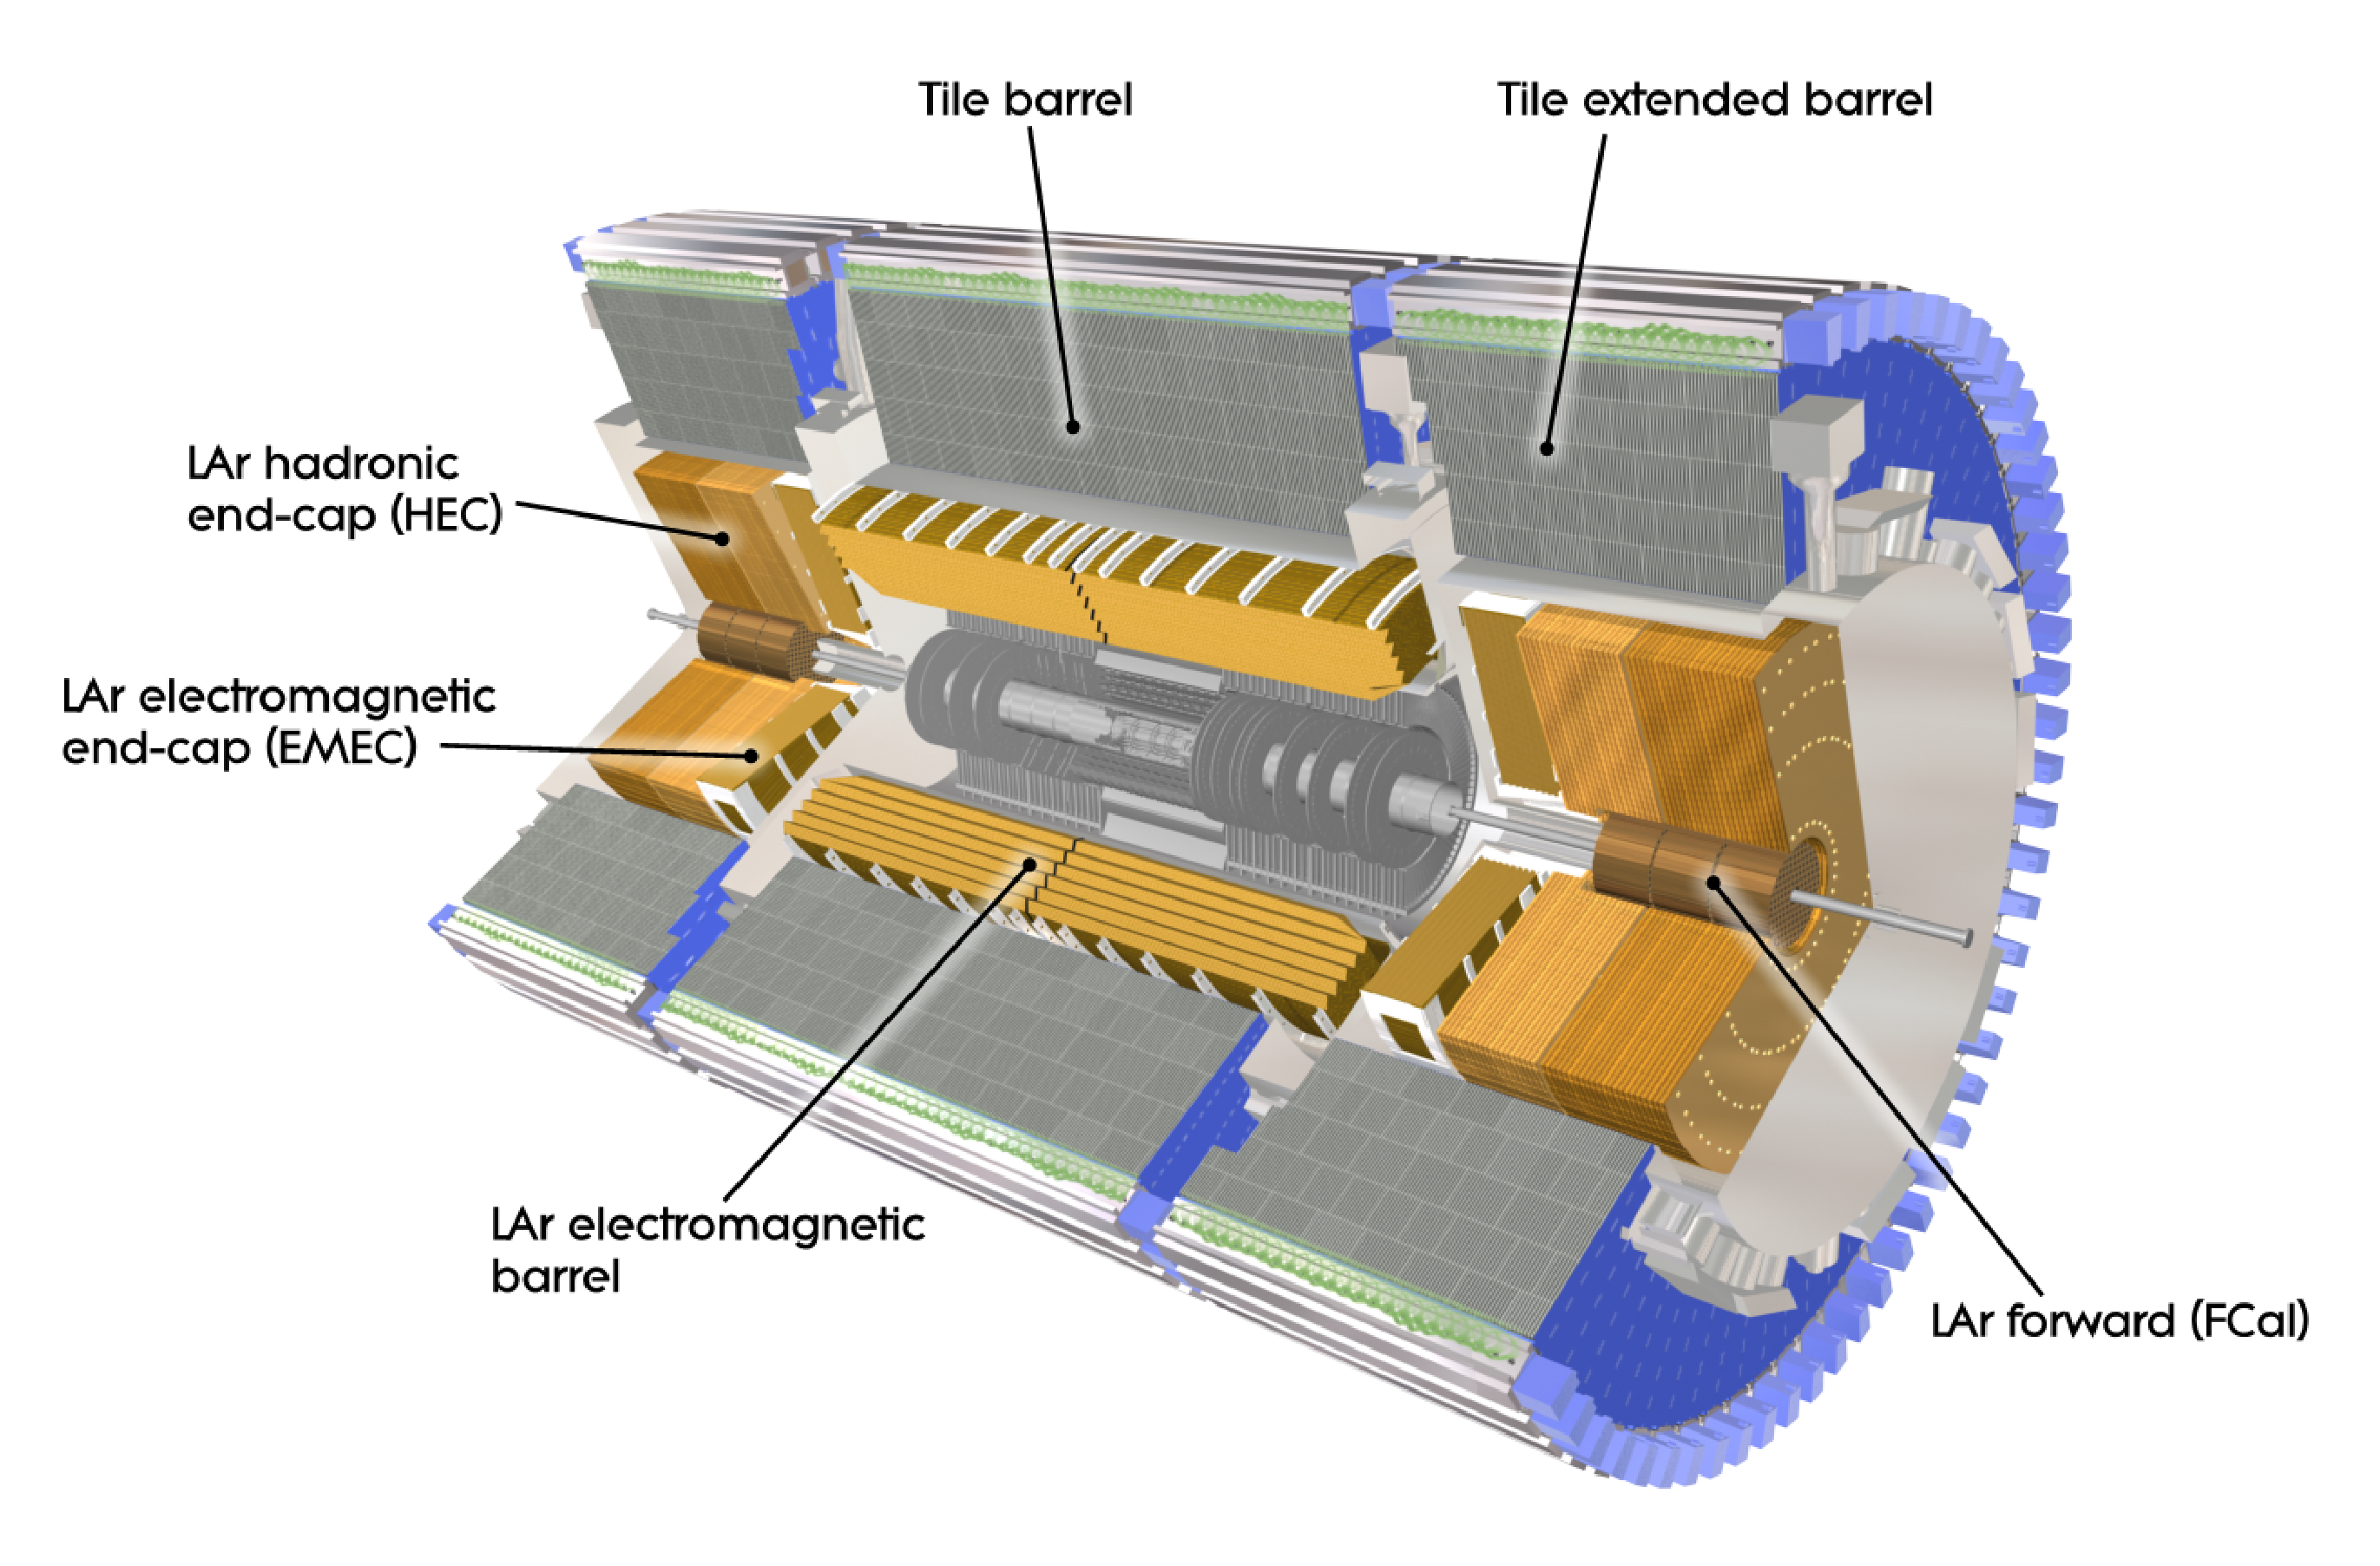
\includegraphics[width=0.995\textwidth]{ATLASdetector/Figures/Calorimeter.eps}
    }
  \end{center}
  \caption[Schematic view of the ATLAS calorimeter system.]{Schematic view of the ATLAS calorimeter system \protect\cite{Evans:2008zzb}.}
  \label{fig:CalorimetersSchema}
\end{figure}

The ATLAS calorimeters provide good containment for electromagnetic and hadronic showers. 
The thickness in the barrel of the EM calorimeter is greater than 22 radiation lengths ($X_0$), while it is greater than $24X_0$ in the end-caps.
An interaction length ($\lambda$) of active material of about 9.7 is found in the hadronic calorimeter barrel, while it increases up to about $10$ in the end-caps.
This thickness ensures an accurate $\met$ measurement.
Figure~\ref{fig:InteractionLengthCalo} shows the thickness in terms of interaction lengths of each layer of the ATLAS calorimeters versus $|\eta|$.

\begin{figure}[!ht]
  \begin{center}
    \mbox{
      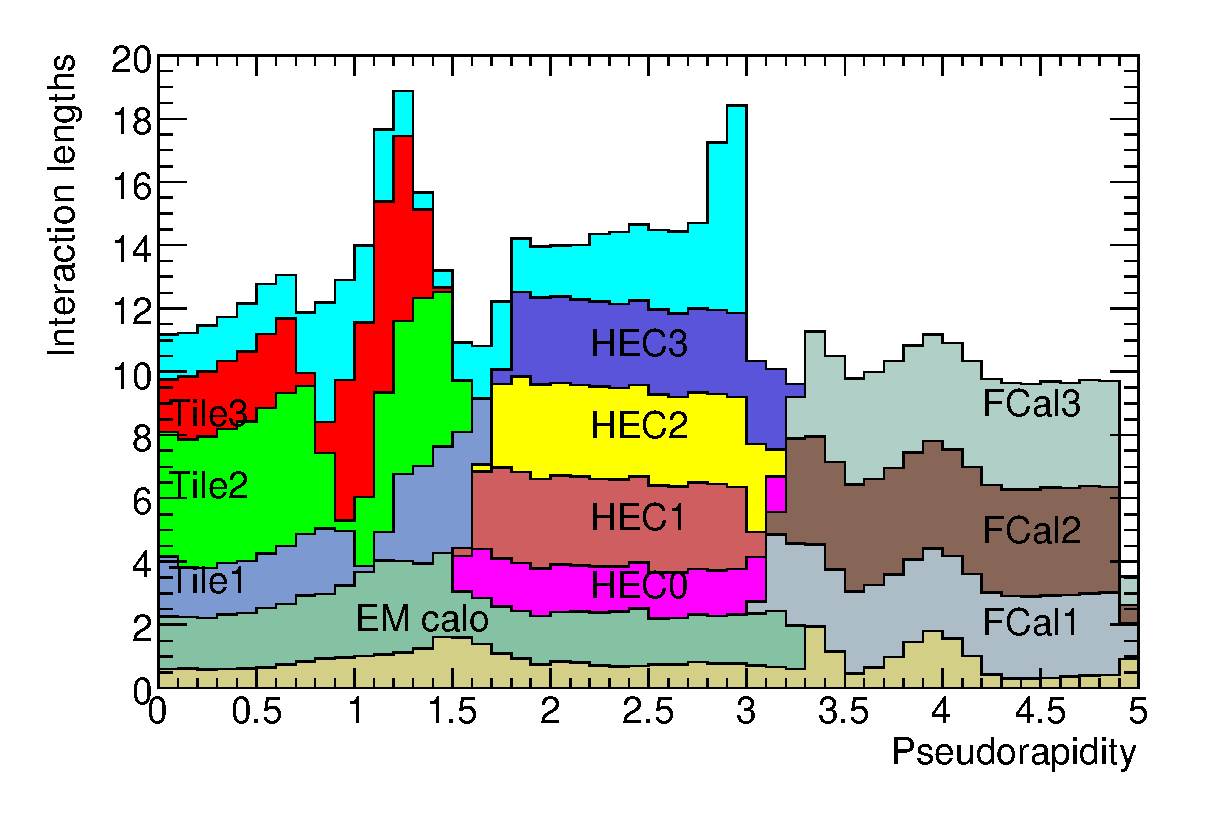
\includegraphics[width=0.995\textwidth]{ATLASdetector/Figures/CalorimeterRadiationLength.eps}
    }
  \end{center}
  \caption[Cumulative amount of material in the calorimeters and the first layer of the muon spectrometer.]{Cumulative amount of material, in units of interaction length, as a function of $|\eta|$, in front of the electromagnetic calorimeters, in the electromagnetic calorimeters themselves, in each hadronic compartment and the total amount at the end of the active calorimetry. Also shown for completeness is the total amount of material in front of the first active layer of the muon spectrometer (up to $|\eta|<3.0$) \protect\cite{Aad:2008zzm}.}
  \label{fig:InteractionLengthCalo}
\end{figure}


\subsubsection{Electromagnetic calorimeter}
    \label{subsubsec:LAr}

The electromagnetic calorimeter is a lead-LAr detector with accordion-shaped kapton electrodes and lead absorber plates over its full coverage.
Charged particles traversing the active material create couples of ions and electrons, that drift in opposite directions due to the presence of an electric field, and are collected by the Kapton electrodes. 
Different geometries for the Kapton electrodes have been used in order to minimize the calorimeter loss. 
For this reason, an accordion geometry has been used, which provides $\phi$ symmetry without azimutal cracks. 
Figure~\ref{fig:CalorimeterModules} (left) provides a schema of a LAr module.
The EM calorimeter is divided into a barrel part (EMB, $|\eta|<1.475$) and two end-caps (EMEC, $1.375<|\eta|<3.2$). 
All the LAr detectors are segmented transversely and divided in four layers in depth (a presampler and three layers), corresponding to a total of 182,468 cells.
The granularity of the different layers versus their $|\eta|$ coverage is shown in Table \ref{tab:LArGranularity}.
Located behind the EMEC is a copper-liquid argon hadronic end-cap calorimeter ($1.5<|\eta|<3.2$) and a copper/tungsten-liquid argon forward calorimeter, which will be explained in more detail in subsection~\ref{subsubsec:TileCal}.

\begin{table}[!ht]
  \begin{center}
    \begin{small}
      \setlength{\tabcolsep}{0.0pc}
      \begin{tabular*}{\textwidth}{@{\extracolsep{\fill}}ccccc}
        \noalign{\smallskip}\hline\hline\noalign{\smallskip}
                                     & \multicolumn{4}{c}{\textbf{EM calorimeter}} \\
                                     & \multicolumn{2}{c}{\textbf{Barrel}} & \multicolumn{2}{c}{\textbf{End-cap}} \\
                                     & $\Delta\eta \times \Delta\phi$ & $|\eta|$ & $\Delta\eta \times \Delta\phi$ & $|\eta|$ \\
        \noalign{\smallskip}\hline\noalign{\smallskip}
        Presampler                   & $0.025\times0.1$               & $<1.52$  &  $0.025\times0.1$              & 1.5-1.8 \\
        \noalign{\smallskip}\hline\noalign{\smallskip}
        \multirow{7}{*}{First layer} & $0.025/8\times0.1$             & $<1.40$  &  $0.050\times0.1$              & 1.375-1.425 \\
                                     & $0.025\times0.025$             & $1.40-1.475$  &  $0.025\times0.1$              & 1.425-1.5 \\
                                     &                                &          &  $0.025/8\times0.1$              & 1.5-1.8 \\
                                     &                                &          &  $0.025/6\times0.1$              & 1.8-2.0 \\
                                     &                                &          &  $0.025/4\times0.1$              & 2.0-2.4 \\
                                     &                                &          &  $0.025\times0.1$              & 2.4-2.5 \\
                                     &                                &          &  $0.1\times0.1$              & 2.5-3.2 \\
        \noalign{\smallskip}\hline\noalign{\smallskip}
        \multirow{3}{*}{Second layer}& $0.025\times0.025$             & $<1.40$  &  $0.050\times0.025$            & 1.375-1.425 \\
                                     & $0.075\times0.025$             & $1.40-1.475$  &  $0.025\times0.025$      & 1.425-2.5 \\
                                     &                                &          &  $0.1\times0.1$              & 2.5-3.2 \\
        \noalign{\smallskip}\hline\noalign{\smallskip}
        Third layer   & $0.050\times0.025$             & $<1.35$  &  $0.050\times0.025$              & 1.5-2.5 \\
        \noalign{\smallskip}\hline\hline\noalign{\smallskip}
      \end{tabular*}
    \end{small}
  \end{center}
  \caption{Granularity versus $\eta$ coverage of the different layers of the electromagnetic LAr calorimeter.}
  \label{tab:LArGranularity}
\end{table}

\begin{figure}[!ht]
  \begin{center}
    \mbox{
      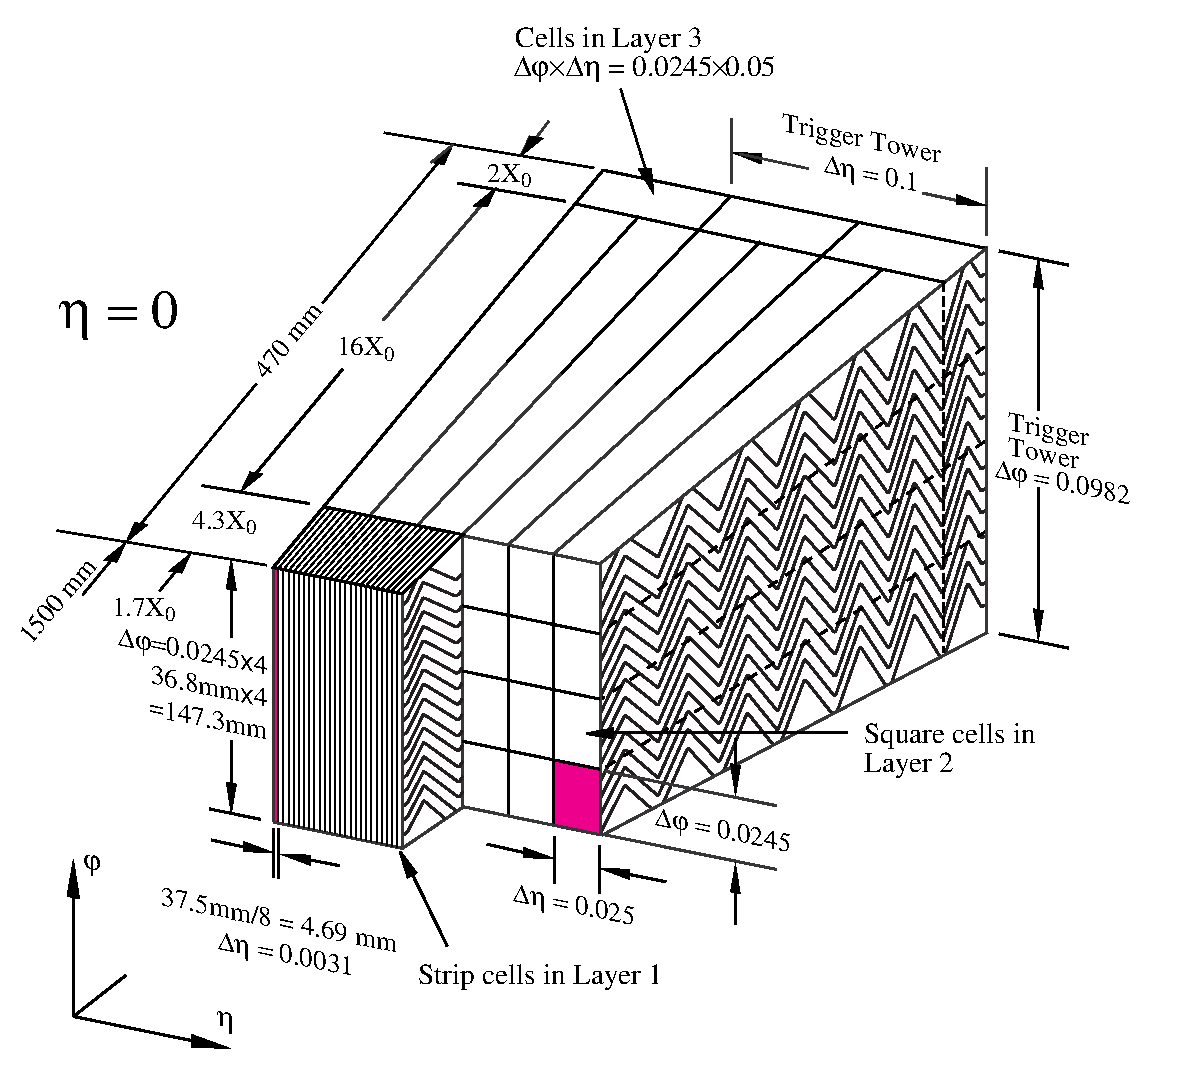
\includegraphics[width=0.495\textwidth]{ATLASdetector/Figures/LAr_Module.eps}
      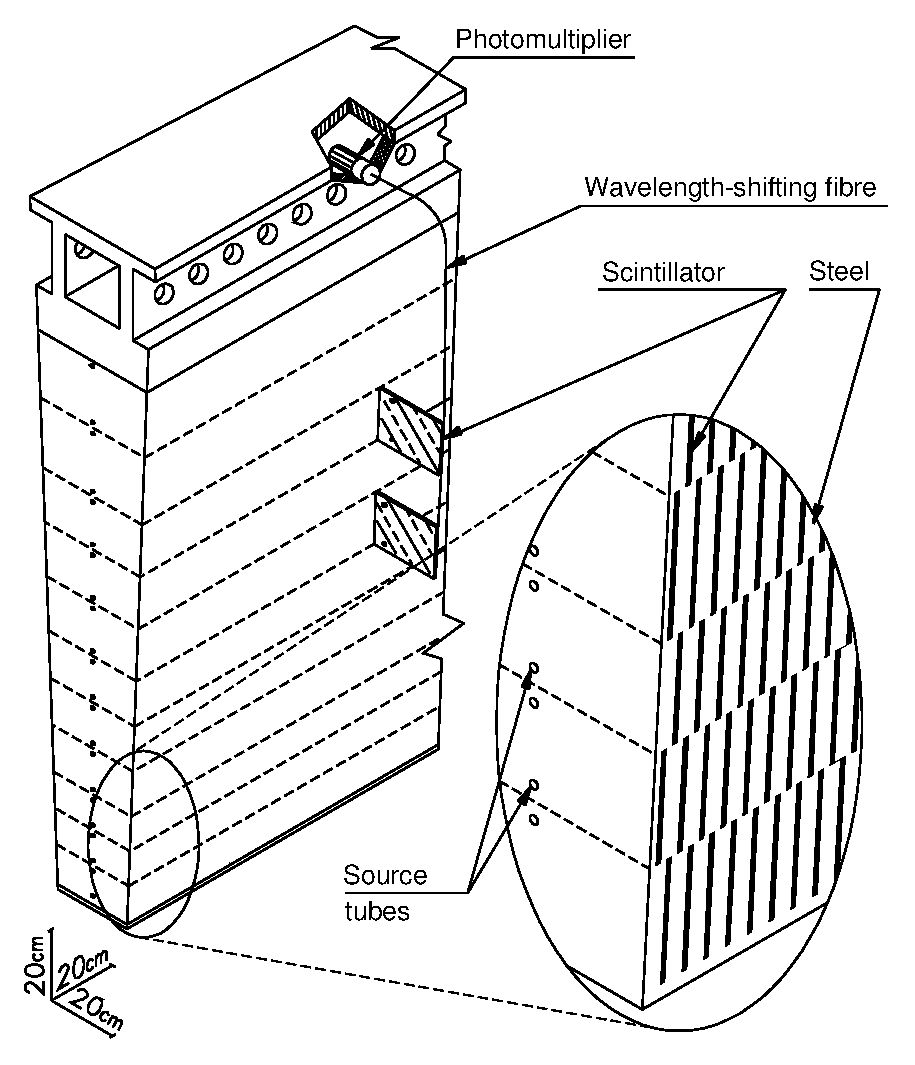
\includegraphics[width=0.495\textwidth]{ATLASdetector/Figures/TileCal_Module.eps}
    }
  \end{center}
  \caption[Schema of LAr and TileCal modules.]{Schema of LAr and TileCal modules~\cite{Aad:2010ai,Aad:2010af}.}
  \label{fig:CalorimeterModules}
\end{figure}

This calorimeter plays a central role in understanding the experimental signatures involving electrons, photons, $\met$, jets and taus.


\subsubsection{Hadronic calorimeter}
    \label{subsubsec:TileCal}

The hadronic calorimeter provides accurate energy and position measurements of isolated hadrons, taus and jets.
It also contributes in particle identification and in muon momentum reconstruction.
The central part of the calorimeter uses scintillating tiles technology, while the end-cap and forward hadronic calorimeter use the same LAr technology as the electromagnetic calorimeter discussed in the previous section.

The {\bf Tile Calorimeter} (TileCal) is placed directly surrounding the electromagnetic calorimeter and is divided into a barrel (LB, $|\eta|<1.0$) and two extended barrels (EB, $0.8<|\eta|<1.7$).
It uses plastic scintillator as the active material and low-carbon steel as the absorber.
Both the LB and the EB are segmented into 64 modules in $\phi$, corresponding to a $\Delta\phi$ granularity of $\unit[0.1]{radians}$.
Radially, each module is further segmented into three layers, which are approximately 1.5, 4.1 and 1.8 $\lambda$ thick for the barrel and 1.5, 2.6 and 3.3 for the extended barrel (as shown in Figure~\ref{fig:InteractionLengthCalo}).
The $\Delta\eta$ segmentation of each module is $0.1$ in the first two radial layers and $0.2$ in the third one.
Wavelength shifting fibers coupled to the tiles on either $\phi$ edge of the cells collect the produced light and are read out by two photomultiplier tubes (PMTs), each linked to one readout channel. 
Figure~\ref{fig:CalorimeterModules} (right) shows a schema of a TileCal module.
Furthermore, located on the inner radius surface of the extended barrel modules, the gap scintillators cover the region of $1.0<\eta<1.2$ while the crack scintillators are located on the front of the LAr end-cap and cover the region $1.2<\eta<1.6$.
Finally, 16 Minimum Bias Trigger Scintillators (MBTS) are located on the front face of the LAr end-cap cryostat and span an $\eta$ range of $2.12<\eta<3.85$.
The number of channels, cells and trigger outputs of the barrels, gap and crack and MBTS of the Tile calorimeter is summarized in Table~\ref{tab:TileCalCells}.
The TileCal related work developed during this PhD Thesis is collected in Appendix~\ref{app:DetectorWork}.

\begin{table}[!ht]
  \begin{center}
    \begin{small}
      \setlength{\tabcolsep}{0.0pc}
      \begin{tabular*}{\textwidth}{@{\extracolsep{\fill}}cccc}
        \noalign{\smallskip}\hline\hline\noalign{\smallskip}
                                     & \textbf{Channels} & \textbf{Cells} & \textbf{Trigger outputs} \\
        \noalign{\smallskip}\hline\noalign{\smallskip}
        Long barrel                  & 5760 & 2880 & 1152 \\
        Extended barrel              & 3564 & 1790 & 768 \\
        Gap and crack                & 480 & 480 & 128 \\
        MBTS                         & 32 & 32 & 32 \\
        \noalign{\smallskip}\hline\noalign{\smallskip}
        Total                        & 9836 & 5182 & 2080 \\
        \noalign{\smallskip}\hline\hline\noalign{\smallskip}
      \end{tabular*}
    \end{small}
  \end{center}
  \caption[Number of channels, cells and trigger outputs of the Tile Calorimeter.]{Number of channels, cells and trigger outputs of the Tile Calorimeter. The gap and crack and MBTS channels are readout in the extended barrel drawers \protect\cite{Aad:2010af}.}
  \label{tab:TileCalCells}
\end{table}

The {\bf Hadronic End-cap Calorimeter} (HEC) is a copper/liquid-argon hadronic end-cap calorimeter which consists of two independent wheels per end-cap, located directly behind the end-cap electromagnetic calorimeter.
They cover the region $1.5<|\eta|<3.2$, and each wheel is divided into two segments in depth.
The wheels are build from parallel copper plates as absorber, interleaved with LAr gaps providing the active medium.

The {\bf Forward Calorimeter} (FCal) is a copper/tungsten-liquid argon calorimeter. 
It is integrated into the end-cap cryostats, and it covers the region $3.1<|\eta|<4.9$.
The FCal consists of three modules per end-cap: the first is made of copper absorber, and is optimized for electromagnetic measurements, while the other two are made of tungsten and measure mainly the energy from hadronic interactions. 
All modules use LAr as active medium.

Table \ref{tab:TileGranularity} illustrates the granularity of each of the hadronic calorimeter layers versus the $|\eta|$ range.

\begin{table}[!ht]
  \begin{center}
    \begin{small}
      \setlength{\tabcolsep}{0.0pc}
      \begin{tabular*}{\textwidth}{@{\extracolsep{\fill}}ccccc}
        \noalign{\smallskip}\hline\hline\noalign{\smallskip}
                                     & \multicolumn{4}{c}{\textbf{Hadronic calorimeter}} \\
                                     & \multicolumn{2}{c}{\textbf{Scintillator tile}} & \multicolumn{2}{c}{\textbf{LAr hadronic}} \\
                                     & Barrel & Extended barrel & \multicolumn{2}{c}{End-cap} \\
        \noalign{\smallskip}\hline\noalign{\smallskip}
        $|\eta|$ coverage                            & $<1.0$         & 0.8-1.7        & 1.5-2.5        & 2.5-3.2 \\
         Number of layers                            & 3              & 3              & \multicolumn{2}{c}{4}       \\
        Granularity ($\Delta\eta \times \Delta\phi$) & $0.1\times0.1$ & $0.1\times0.1$ & \multirow{2}{*}{$0.1\times0.1$} & \multirow{2}{*}{$0.2\times0.2$} \\
        (last layer)                                 & $0.2\times0.1$ & $0.2\times0.1$ &                & \\ 
        \noalign{\smallskip}\hline\hline\noalign{\smallskip}
      \end{tabular*}
    \end{small}
  \end{center}
  \caption{Granularity versus $\eta$ coverage of the different layers of the hadronic calorimeter.}
  \label{tab:TileGranularity}
\end{table}


\subsection{Muon spectrometers}
    \label{subsec:MuonSpectrometers}

The Muon Spectrometer (MS) is surrounding the calorimeters, and is the most outer part of the ATLAS detector, as it is shown in Figure~\ref{fig:MuonSpectrometerSchema}. 
The MS has been designed to identify and measure high momentum muons and consists of four systems that make use of different technologies: Monitored Drift Tubes (MDT), Cathode Strip Chambers (CSC), Resistive Plate Chambers (RPC) and Thin Gap Chambers (TGC).
Table \ref{tab:MuonSpectrometerDetails} summarizes the properties of the muon spectrometer subsystems and their $\eta$ coverage.
The spectrometer is based on the magnetic deflection of muon tracks when they cross the magnetic field produced by the superconducting air-core toroid magnets.

\begin{table}[!ht]
  \begin{center}
    \begin{small}
      \setlength{\tabcolsep}{0.0pc}
      \begin{tabular*}{\textwidth}{@{\extracolsep{\fill}}ccccc}
        \noalign{\smallskip}\hline\hline\noalign{\smallskip}
                                     & \multicolumn{4}{c}{\textbf{Muon spectrometer}} \\
                                     & \textbf{MDT} & \textbf{CSC} & \textbf{RPC} & \textbf{TGC} \\
        \noalign{\smallskip}\hline\noalign{\smallskip}
        \multirow{2}{*}{$|\eta|$ coverage}     & $<2.7$          & \multirow{2}{*}{2.0-2.7} & \multirow{2}{*}{$<1.05$} & 1.05-2.7 \\
                                               & (innermost layer $<2.0$)          &  &  & (1.05-2.4 trigger) \\
         Number of chambers                            & 1150           & 32            & 606            & 3588       \\
         Number of channels                            & 354000         &310000         & 373000         & 318000     \\
         \multirow{2}{*}{Function}                     & Precision      & Precision& Triggering, & Triggering, \\
                                                       & tracking       & tracking & $\phi$-coordinate & $\phi$-coordinate \\
        \noalign{\smallskip}\hline\hline\noalign{\smallskip}
      \end{tabular*}
    \end{small}
  \end{center}
  \caption{Properties and $\eta$ coverage of the different Muon spectrometer subsystems.}
  \label{tab:MuonSpectrometerDetails}
\end{table}

\begin{figure}[!ht]
  \begin{center}
    \mbox{
      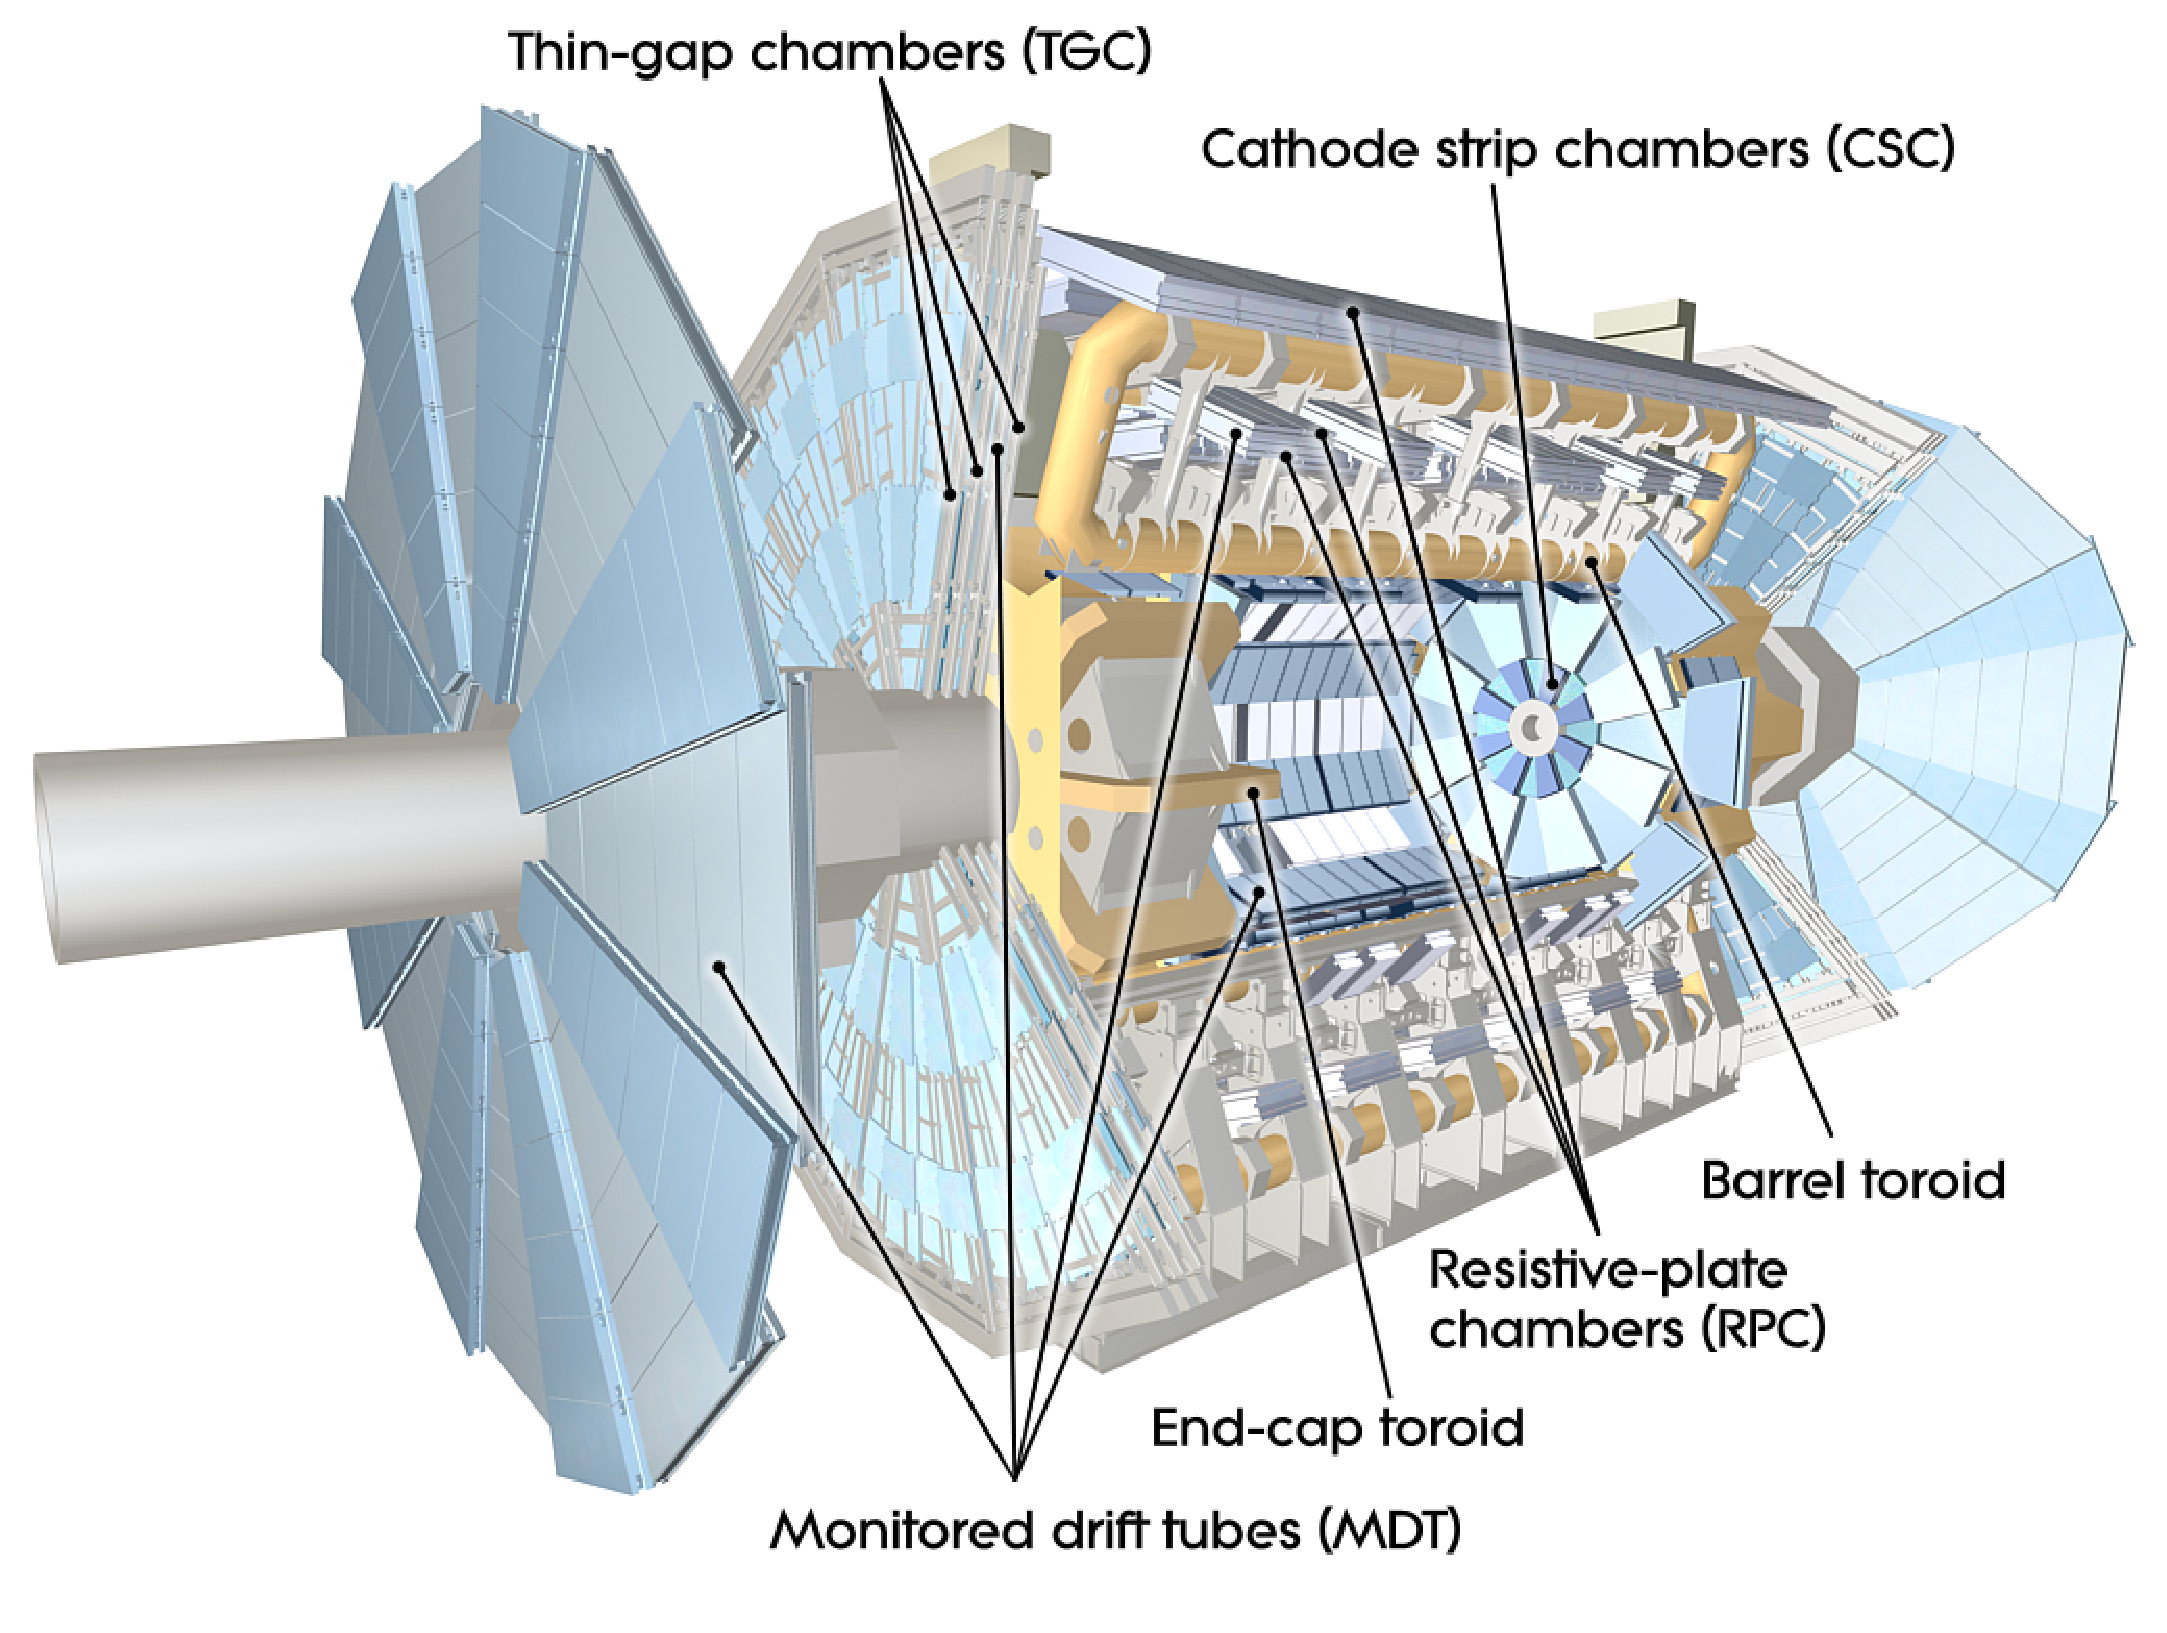
\includegraphics[width=0.995\textwidth]{ATLASdetector/Figures/MuonSystem.eps}
    }
  \end{center}
  \caption[Schematic view of the ATLAS muon spectrometer.]{Schematic view of the ATLAS muon spectrometer \cite{Evans:2008zzb}.}
  \label{fig:MuonSpectrometerSchema}
\end{figure}

The air-core toroid magnet is separated in three parts: one covering the central pseudo-rapidity range ($|\eta|<1.5$) producing a $\unit[0.5]{T}$ field, and the other two at higher pseudo-rapidity ($|\eta|>1.5$), generating a $\unit[1]{T}$ field.
Each of the magnets consist of eight coils assembled radially around the beam axis, to create a magnetic field almost orthogonal to the muon trajectories and bends them along the $\theta$ angle.

The {\bf Monitor Drifted Tubes} provide a precision coordinate measurement in the bending direction of the air-core toroidal magnet, and therefore provide the  muon momentum measurement for $|\eta|<2.7$.
The basic detection element is a cylindrical aluminum drift tube filled with gas and a central wire at a high potential. The muons passing through the tubes ionize the gas and produce charges that are collected on the wire.

The {\bf Cathode Strip Chambers} are used at high pseudo-rapidities to help confronting the demanding rate and background conditions.
They are multiwire proportional chambers with cathodes segmented into strips.

The {\bf Resistive Plate Chambers} (in the barrel) and the {\bf Thin Gap Chambers} (in the end-caps) are trigger chambers that can provide bunch-crossing identification, well-defined $\pt$ thresholds and they can measure the muon coordinate in the $\phi$ direction.


\subsection{Trigger system}
    \label{subsec:TriggerSystem}

The purpose of the trigger system is to reduce the input rate from several MHz to about $\unit[400]{Hz}$ for recording and offline processing.
This limit is equivalent to an average data rate of about $\unit[300]{MB/s}$, which is the maximum that the computer resources and the offline storage can handle.
For each bunch crossing, the trigger system verifies if at least one of hundreds of conditions (triggers) are satisfied.
Most of them are based on identifying combinations of candidate physics objects such as electrons, muons or jets, but there are also triggers for inelastic $\pp$ collisions (minimum bias) and triggers based on global event properties, such as $\sum\et$ or $\met$.

The system has three levels; the first level (L1) is a hardware-based system using information from the calorimeter and muon sub-detectors. 
The second (L2) and the third (Event Filter, EF) together are software-based systems that use information from all sub-detectors. 
They are called the High Level Trigger (HLT).

\begin{figure}[!ht]
  \begin{center}
    \mbox{
      \includegraphics[width=0.995\textwidth]{ATLASdetector/Figures/TriggerSystem.eps}
    }
  \end{center}
  \caption[Schema of the ATLAS trigger system.]{Schema of the ATLAS trigger system~\protect\cite{Aad:2012xs}.}
  \label{fig:TriggerSchema}
\end{figure}

Figure~\ref{fig:TriggerSchema} shows a schema of the ATLAS trigger system.
Detector signals are stored in front-end pipelines pending a decision from the L1 trigger system, which is implemented in fast electronics in order to minimize the latency time.
In addition to performing the first selection step, the L1 triggers identify Regions of Interest (RoIs) within the detector to be investigated by the HLT.
It is designed to reduce the rate to a maximum of $\unit[75]{kHz}$.
The HLT consists of farms of processors connected by fast dedicated networks.
When an event is accepted by the L1 trigger, data from each detector are transferred to the detector-specific Readout Buffers (ROB), which store the event in fragments pending the L2 decision.
The L2 selection is based on fast custom algorithms processing partial event data within the RoIs identified by L1.
The L2 processors request data corresponding to detector elements inside each RoI, reducing the amount of data to be transferred.
The L2 triggers reduce the rate to approximately $\unit[3]{kHz}$ with an average processing of $\unit[40]{ms}$ per event.
Finally the EF is based on offline algorithms and it is designed to reduce the rate up to $\unit[400]{Hz}$. 
It uses the full information of the events passing the L2.


\subsection{Luminosity measurement}
    \label{subsec:LuminosityMeasurement}

An accurate measurement of the luminosity is a key component for all physics analyses. 
For cross section measurements, the uncertainty on the delivered luminosity is one of the major systematic uncertainties, but also searches for new physical phenomena beyond the Standard Model rely on accurate information about the delivered luminosity to evaluate background levels and determine sensitivity to the signatures of new phenomena.
The ATLAS luminosity is determined with a number of sub-detectors, using different methods and algorithms \cite{Aad:2013ucp}.

The instantaneous luminosity, $\InstLumi$, can be expressed in terms of accelerator parameters, as:

\begin{equation}
  \InstLumi = \frac{n_{b} f_{r} n_{1} n_{2}}{2\pi \Sigma_{x} \Sigma_{y}}, 
  \label{LumiDefinitionAccelerator}
\end{equation}

\noindent where $n_{1}$ and $n_{2}$ are the bunch populations (protons per bunch) in beams~1 and~2 respectively, $f_{r}$ is the revolution frequency of the LHC, $n_{b}$ are the bunch pairs colliding in each revolution and $\Sigma_{x}$ and $\Sigma_{y}$ characterize the horizontal and vertical convolved beam widths, extracted in a {\emph van der Meer} (vdM) scan\footnote{Also known as beam-separation scan}.
In a vdM scan, the observed event rate is recorded while scanning the two beams across each other first in the horizontal ($x$) and then in the vertical ($y$) directions. This yields two bell-shaped curves, with the maximum rate at zero separation, from which the $\Sigma_{x}$ and $\Sigma_{y}$ values can be extracted.
Then, the total absolute luminosity can be computed with Equation~\ref{LumiDefinitionAccelerator}.

The luminosity can be re-written as:

\begin{equation}
  \InstLumi = \frac{R_{\text{inel}}}{\sigma_{\text{inel}}} = 
  \frac{\averageIntXing n_b f_r}{\sigma_{\text{inel}}} = 
  \frac{\averageIntXing_{\text{vis}} n_b f_r}{\sigma_{\text{vis}}}, 
  \label{LumiDefinition}
\end{equation}

\noindent where $R_{\text{inel}}$ is the rate of inelastic collisions, $\sigma_{\text{inel}}$ is the $\pp$ inelastic cross-section, $\averageIntXing$ is the average number of interactions per bunch crossing (BC) and $\sigma_{\text{vis}} = \epsilon\sigma_{\text{inel}}$, where $\epsilon$ is the efficiency of a particular detector and algorithm.

By measuring simultaneously the peak collision rate (at zero beam separation), $\averageIntXing_{\text{vis}}^{\text{MAX}}$, and the corresponding peak absolute luminosity, $\InstLumi^{\text{MAX}}$ (using Eq. \ref{LumiDefinitionAccelerator}), the constant $\sigma_{\text{vis}} = \epsilon\sigma_{\text{inel}}$ can be determined by:

\begin{equation}
  \sigma_{\text{vis}} = \averageIntXing_{\text{vis}}^{\text{MAX}} \frac{n_{b} f_{r}}{\InstLumi^{\text{MAX}}}.
  \label{LumiVisibleXSection}
\end{equation}

Therefore, after the calibrations from the vdM scan, the ATLAS luminosity can be directly computed with Equation~\ref{LumiDefinition}, once $\averageIntXing_{\text{vis}}$ has been determined.
In order to measure this quantity with a sub-detector, ATLAS primarily uses event counting algorithms for which the number of events that satisfies a given criteria are compared to the total number of bunch crossings.
In a vdM scan $\averageIntXing_{\text{vis}} \muchless 1$, and the average number of visible inelastic interactions per BC is given by the expression:

\begin{equation}
  \averageIntXing_{\text{vis}} = \frac{N}{N_{\text{BC}}},
  \label{LumiVisibleMuSmall}
\end{equation}

\noindent where $N$ is the number of events that satisfies the event selection criteria during a given time interval and $N_{\text{BC}}$ is the total number of bunch crossings during the same interval.

\cleardoublepage

\chapter{Reconstruction of physics objects}
    \label{chapter:ReconstructionOfObjects}

This chapter describes the reconstruction of the main physics objects that are relevant for the analysis presented in this Thesis.
The identification, reconstruction and calibration of electrons, muons, jets and missing transverse energy is discussed in detail.

\section{Electrons}
    \label{sec:ElectronReco}

In the following, the electron reconstruction and identification will be described.
The reconstruction step is used to define the electron candidates, while the identification selects electron samples with different purities.

\subsection{Electron reconstruction}
    \label{subsec:ElectronReconstruction}

The electron reconstruction can be divided into central and forward.
In the central region, $|\eta|<2.47$, the electron reconstruction starts from energy deposits (clusters) in the electromagnetic calorimeter that are associated to reconstructed tracks of charged particles in the Inner Detector.
The reconstruction of the electron clusters is based on a fixed-size sliding window algorithm \cite{Lampl:2008zz}.

The tracks are extrapolated from their last measurement point in the inner detector to the second layer of the EM calorimeter and the coordinates from the impact point are then compared to those of the seed cluster.
The cluster matching is performed if at least one track is matched to the seed cluster.
In the case where several tracks are matched to the same cluster, tracks with silicon hits are preferred and the one with the smallest $\Delta R$ distance to the seed cluster is chosen.

The four-momentum of the central electrons is computed using the information from both the final cluster and the best track matched to the original seed cluster.
While the energy is given entirely by the cluster energy, the $\eta$ and the $\phi$ directions are taken from the corresponding track parameters at the vertex.

In the forward region, $2.5 < |\eta| < 4.9$, there are no tracking detectors. Therefore, the electron candidates are reconstructed only from energy deposits in the calorimeters. These clusters are built using a topological clustering algorithm, that will be explained in Section~\ref{sec:JetReco}.

\subsection{Electron identification}
    \label{subsec:ElectronIdentification}

The electron identification aims to provide good separation between isolated electrons and jets faking electrons.
It consist of a cut-based selection on variables that use calorimeter, tracking and combined calorimeter and tracker information.
Three sets of reference selection criteria have been defined with increasing background rejection power: \textit{loose}, \textit{medium} and \textit{tight}, as described in Ref.~\cite{Aad:2011mk}.
The shower shape variables calculated in the second EM calorimeter layer and hadronic leakage variables are used in the loose selection.
These shower shape variables are binned in $\eta$ and $\met$, allowing a proper handling of correlations between variables and assuring the highest efficiency for a given jet rejection \cite{Aad:2014fxa}.
Cuts on the first EM calorimeter layer variables, track quality requirements and track-cluster matching are added in the medium selection.
Finally, in the tight selection, the track quality requirements are tightened.
For the analysis presented in this Thesis, only electrons following the \textit{medium} identification criteria are considered.


\subsection{Electron energy corrections}
    \label{subsec:ElectronEnergyCorrections}

The reconstructed electron energy in data is tuned to reproduce the $Z$ mass peak central value according to the $Z$ mass world average by applying extra corrections as a function of $|\eta|$ \cite{Aad:2011mk}:

\begin{equation}
E_{\text{corrected}} = \frac{E}{1+\alpha},
\label{eq:ElectronEnergyCalibration}
\end{equation}

\noindent where $\alpha$ measures the residual miscalibration. The values of $\alpha$ are within $\pm 2 \%$ in the barrel region and within $\pm 5 \%$ in the forward regions.
The calibrated electron energy scale is further validated with electron candidates from $J/\psi\rightarrow ee$ events in data, and determined with a precision of 0.3--1.6\% in the central region over $|\eta|<2.47$, for different $|\eta|$ values \cite{Aad:2014nim}.

\section{Muons}
    \label{sec:MuonReco}

This section presents the muon reconstruction and identification in ATLAS, which mainly relies on the information extracted from the Inner Detector and the Muon spectrometer. 


\subsection{Track reconstruction}
    \label{subsec:MuonTrackReconstruction}

The tracks of the muon candidates are reconstructed independently in the ID and the MS.
Hits in each station of the Muon Spectrometer are combined to build track segments up to $|\eta|<2.7$.
A similar approach is followed in the inner detector, where the pattern recognition uses space points from the pixel and SCT clusters to generate seeds, which are then extended into the TRT.

\subsection{Muon identification}
    \label{subsec:MuonIdentification}

In ATLAS, the muon identification is performed according to several reconstruction criteria, which leads to different muon ``types''.
These types are defined based on the available information from the ID, the MS and different calorimeter sub-detector systems~\cite{Aad:2014rra}:

\begin{itemize}
\item{Stand-alone (SA):} The muon trajectory is only reconstructed in the muon spectrometer. The direction of flight and the impact parameter of the muon at the interaction point are determined by extrapolating the spectrometer track back to the beam line.
\item{Combined muon (CB):} The momentum of the stand-alone muon is combined with the momentum measured in the ID, which also provides information about the impact parameter of the muon trajectory with respect to the primary vertex.
\item{Segment tagged (ST):} A trajectory in the inner detector is identified as a muon if the trajectory extrapolated to the muon spectrometer can be associated with straight track segments in the precision muon chambers.
\item{Calorimeter tagged (CaloTag):} A trajectory in the ID is identified as a muon if the associated energy depositions in the calorimeters is compatible with the hypothesis of a minimum ionizing particle.
\end{itemize}

The analysis described in this Thesis uses combined muons and segment tagged muons, reconstructed with the \textit{staco} reconstruction chain, as described in Ref.~\cite{Hassani:2007cy}.
Combined muons are the highest purity muon candidates.
Tagged muons give additional efficiency, as they can recover muons which did not cross enough precision chambers to allow an independent momentum measurement in the Muon Spectrometer.

The reconstructed muon momentum in data is tuned to reproduce the $Z$ and $J/\Psi$ masses as it was done for electrons, and needs to be studied separately in the ID and the MS.
The dimuon invariant mass resolution of combined muons is found to vary between 2 and 3 GeV, as a function of $|\eta|$. 


\section{Jets}
    \label{sec:JetReco}

In hard interactions, quarks and gluons result in showers of collimated particles, called \textit{jets}.
A well-defined jet algorithm is needed in order to establish a correspondence between observables at partonic, hadronic and detector level.
Jets are reconstructed using the $\akt$ algorithm, described in the following.


\subsection{Jet finding algorithm}
    \label{subsec:JetClusteringAlgorithm}


The $\akt$~\cite{Cacciari:2008gp} is a sequential recombination algorithm, and is the default jet finding algorithm in the LHC experiments.
It starts from an input list of four-vectors, which can be either particles from the $\pp$ interactions simulated in the MC with a lifetime longer than 10~ps (\emph{truth constituents}), reconstructed charged particle tracks associated with the reconstructed primary collision vertex (\emph{track constituents}), or energy depositions in the ATLAS calorimeters (\emph{calorimeter constituents}).
The jet reconstruction in ATLAS is summarized in Figure~\ref{fig:JetReconstructionOverview}.

\begin{figure}[!ht]
  \begin{center}
    \mbox{
      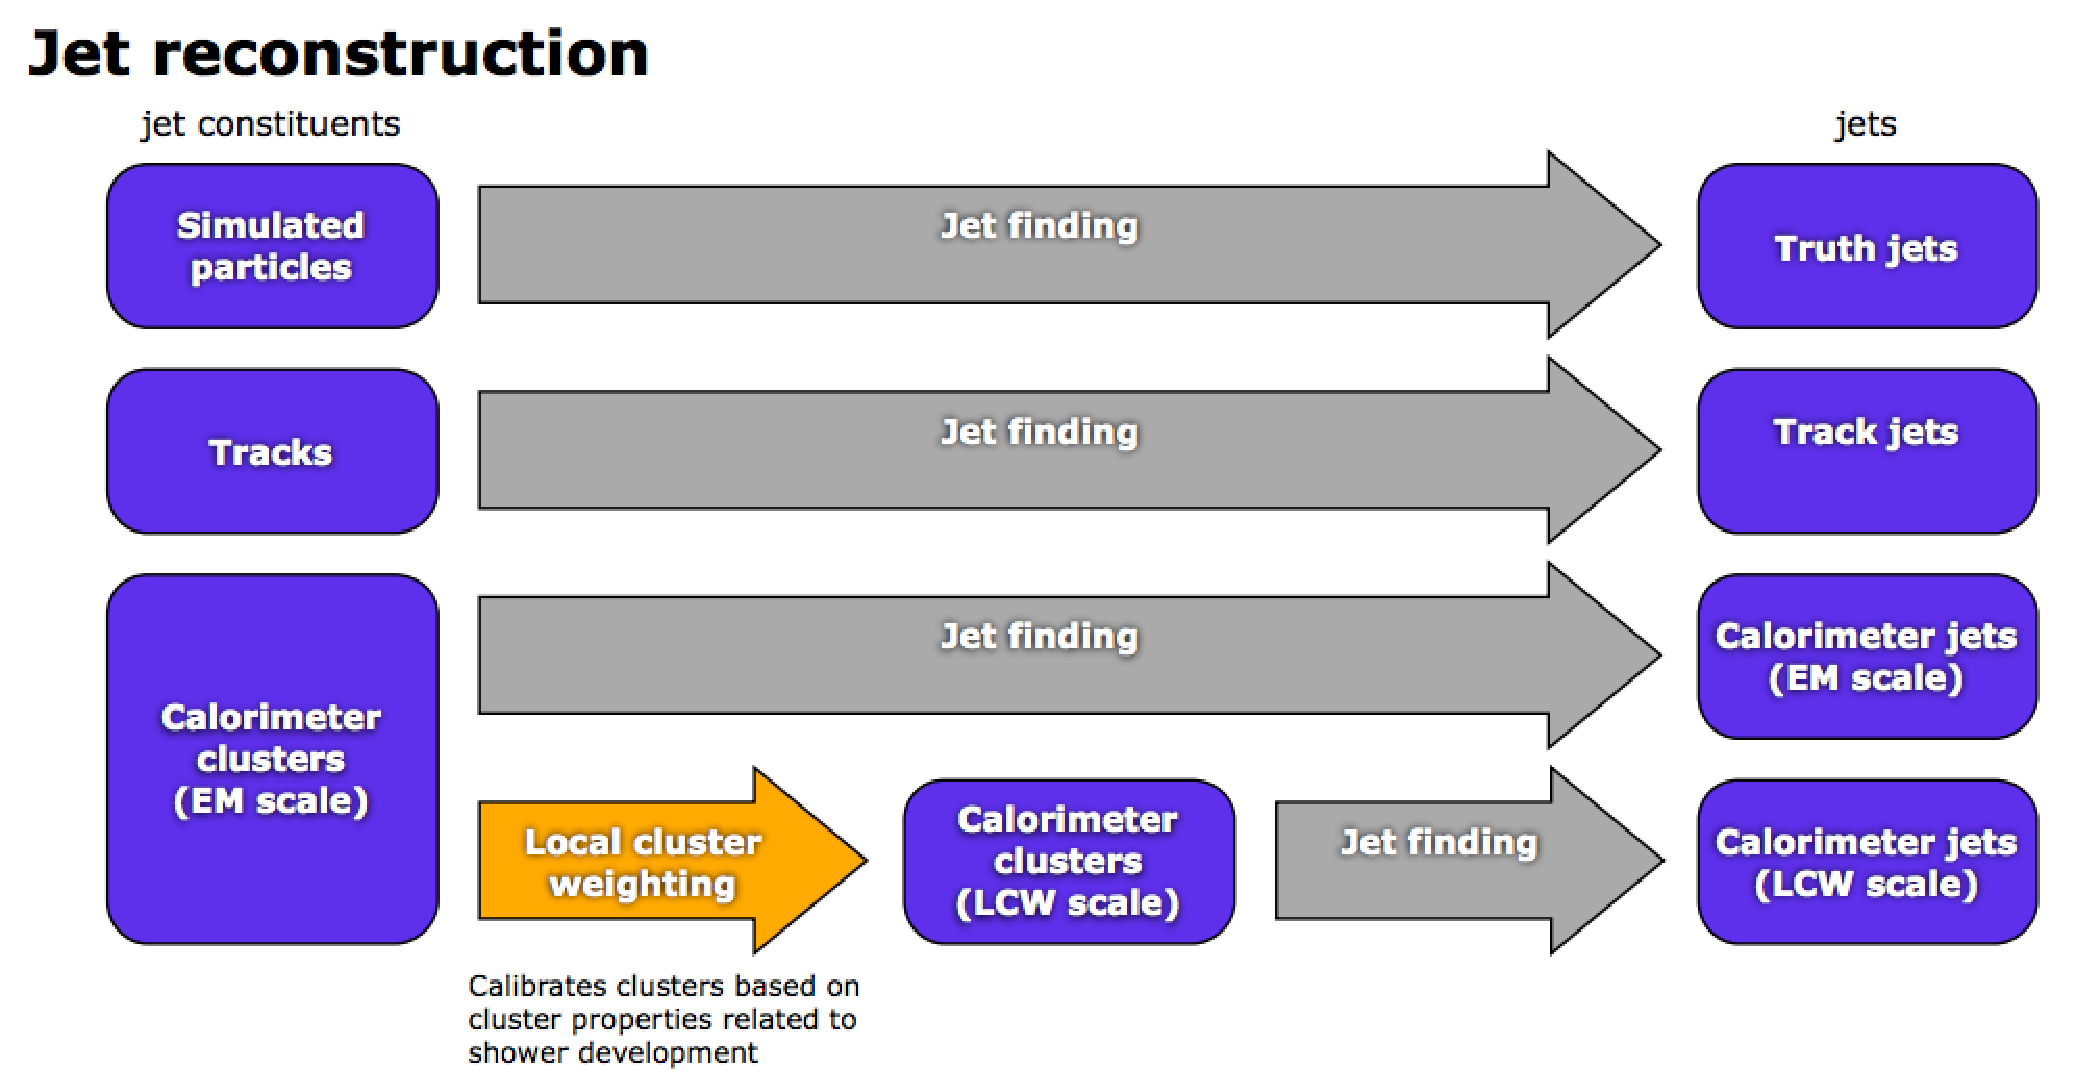
\includegraphics[width=0.995\textwidth]{ObjectReconstruction/Figures/JetReconstructionOverview.eps}
    }
  \end{center}
  \caption[Overview of the ATLAS jet reconstruction.]{Overview of the ATLAS jet reconstruction~\cite{Aad:2014bia}.}
  \label{fig:JetReconstructionOverview}
\end{figure}

For all the input constituents, the $\akt$ algorithm computes the quantities:

\begin{subequations}
    \begin{equation}
        d_{ij} = \min\left( \frac{1}{k_{ti}^{2}}, \frac{1}{k_{tj}^{2}} \right) \frac{\Delta R_{ij}^{2}}{R^2}
        \label{eq:AntiKt_dij}
    \end{equation}
    \begin{equation}
        d_{iB} = \frac{1}{k_{ti}^{2}},
        \label{eq:AntiKt_diB}
    \end{equation}
\end{subequations}

\noindent where $\Delta R_{ij}^{2} = (\eta_i - \eta_j)^2 + (\phi_i - \phi_j)^2$, $R$ is a parameter of the algorithm that approximately controls the size of the jet and $k_{ti}$ is the transverse momentum of the constituent $i$.
Here, $d_{ij}$ is the ``distance'' between the constituents $i$ and $j$, while $d_{iB}$ is the distance between the constituent $i$ and the beam, introduced to separate constituents coming from the interactions from proton remnants.

The $\akt$ jet clustering algorithm proceeds by identifying the smallest of the distances. 
If the smallest distance is a $d_{ij}$, it recombines the entities $i$ and $j$, while if the smallest distance is $d_{iB}$, the algorithm calls $i$ a jet and removes it from the list of entities.
The method used to recombine the different constituents is called \emph{recombination scheme}.
In ATLAS, the $E$-scheme is used, in which the four-momentum of the recombined object is defined by the vectorial sum of the four-momenta of its constituents.
After recombination, the distances are recalculated with the remaining objects, and the procedure repeated until no entities are left.

The $\akt$ algorithm defines jets with a well-defined conical shape, thus allowing robust pileup corrections.
Jets are defined with a minimum transverse momentum threshold $p_T^{\text{jet}}$, used as a scale to separate soft from hard interactions.
Figure \ref{fig:JetTopoClusterAntiKt} (left) illustrates the clustering of hard and soft particles into jets when the $\akt$ algorithm is applied.

\begin{figure}[!ht]
  \begin{center}
    \mbox{
      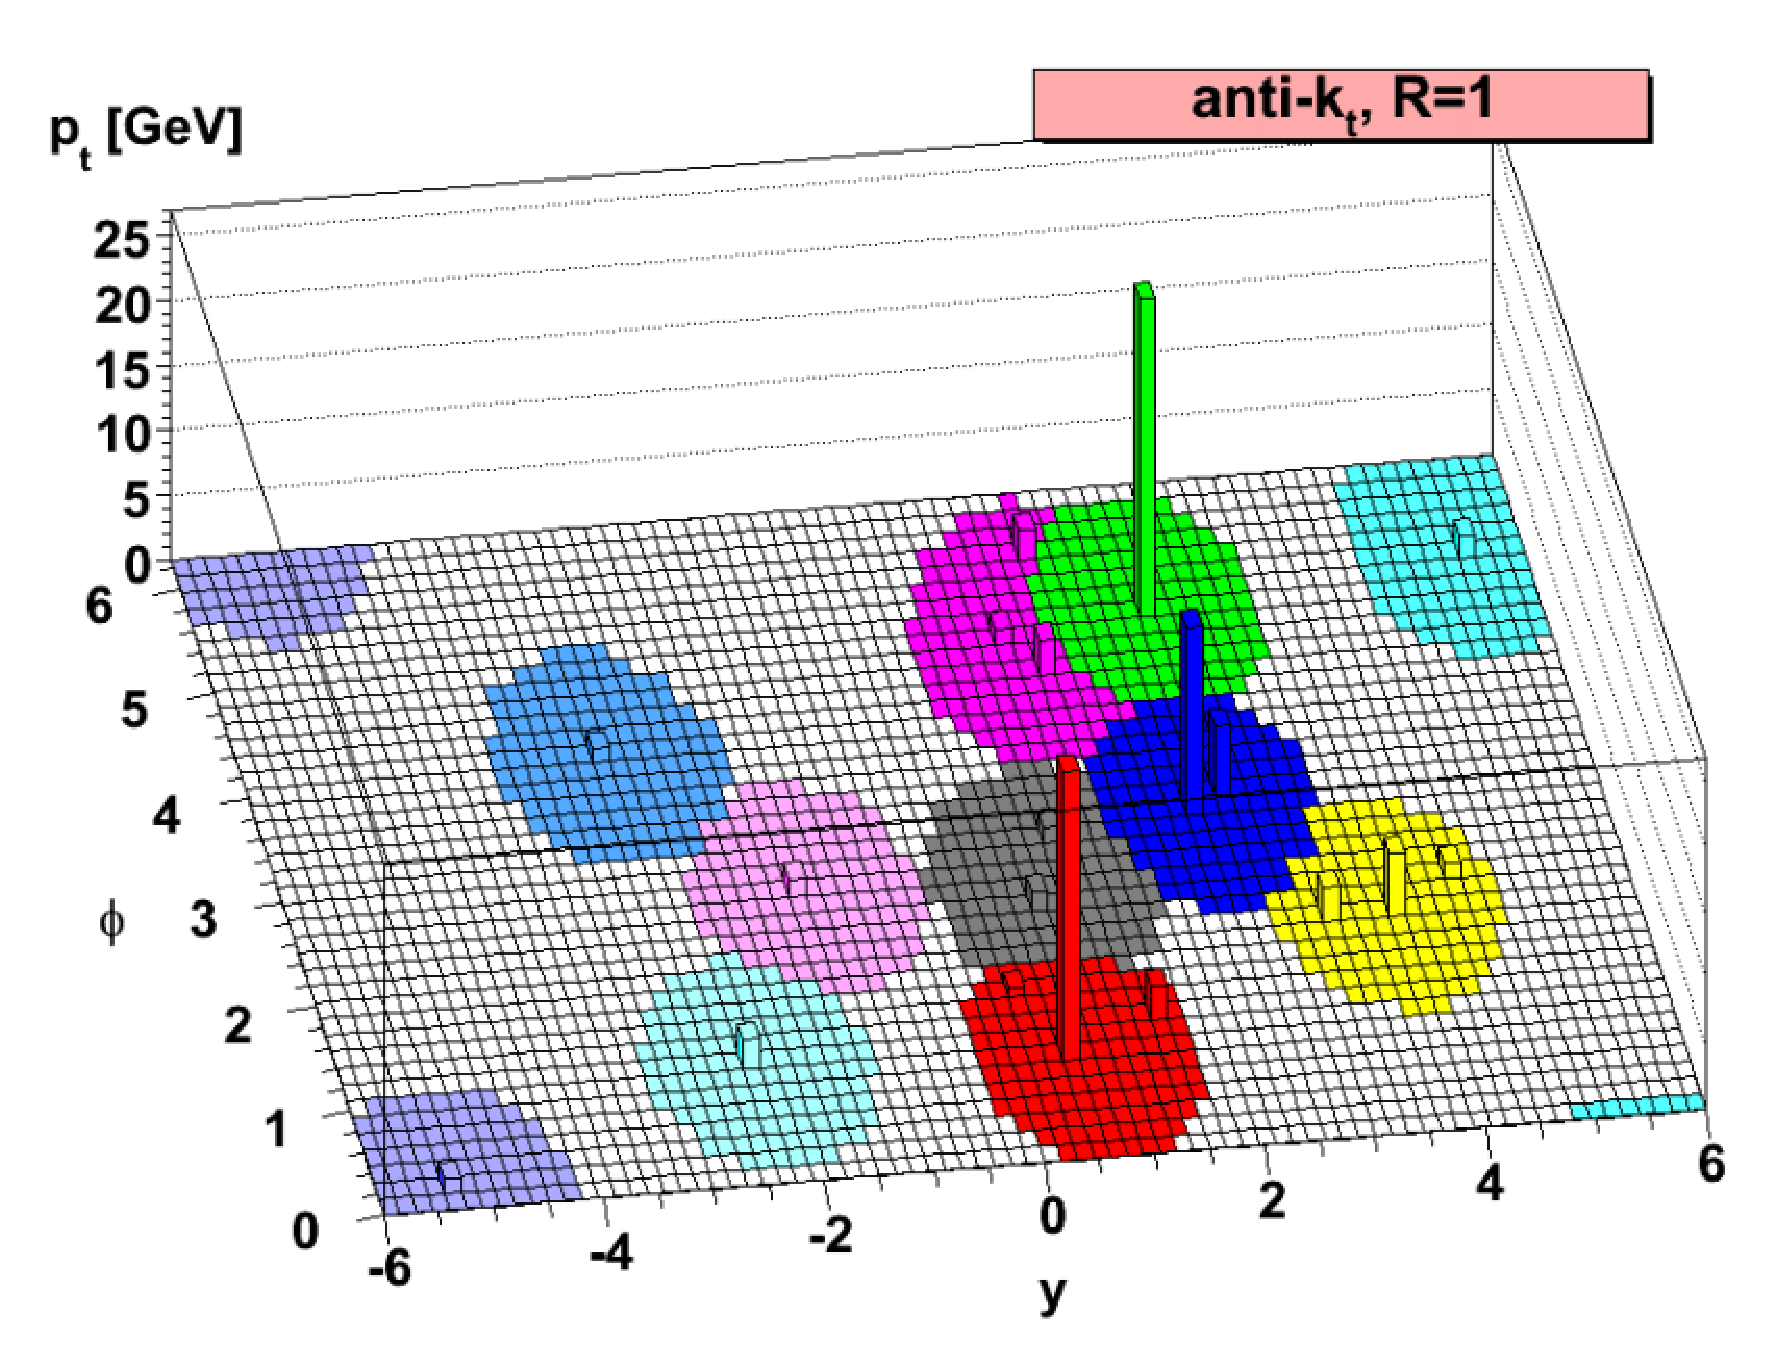
\includegraphics[width=0.495\textwidth]{ObjectReconstruction/Figures/JetAntiKt.eps}
      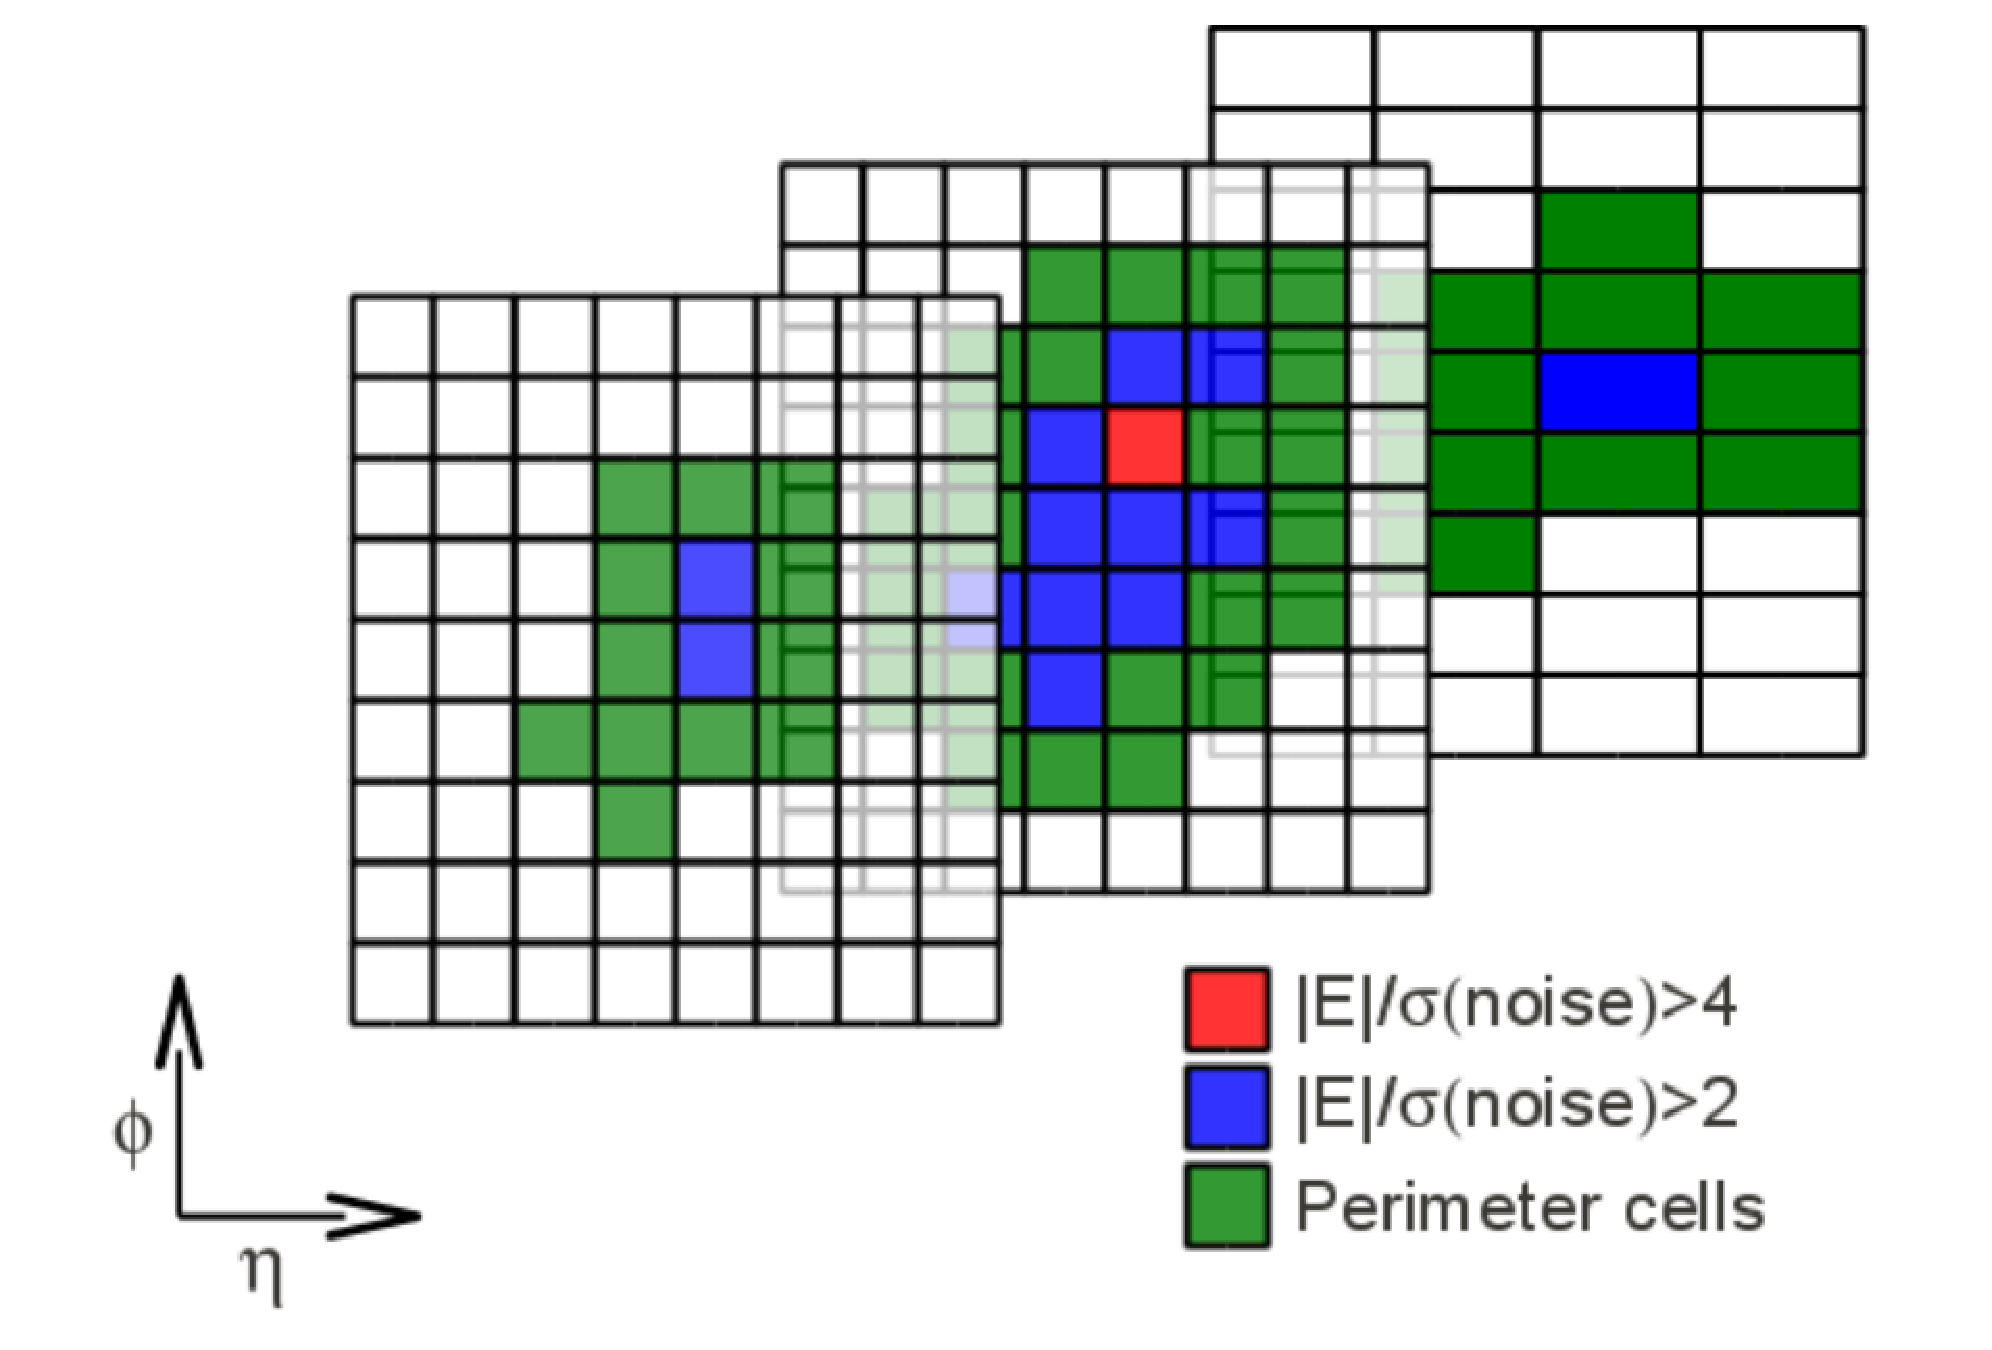
\includegraphics[width=0.495\textwidth]{ObjectReconstruction/Figures/JetClusterFormation.eps}
    }
  \end{center}
  \caption[Illustration of the ``active'' catchment area of the $\akt$ algorithm (left). Topo-cluster formation in the three hadronic layers in the barrel and $\akt$ jet algorithm representation (right).]{
  Illustration of the clustering of the jets with the $\akt$ algorithm~\protect\cite{Cacciari:2008gp} (left).
    Grid representing calorimeter cells, showing topo-cluster formation in the three hadronic layers in the barrel (right). 
  }
  \label{fig:JetTopoClusterAntiKt}
\end{figure}



\subsection{Cluster formation}
    \label{subsec:JetClusterFormation}

The calorimeter constituents mentioned in the previous section are reconstructed with the topological clustering (topo-cluster) algorithm \cite{Lampl:2008zz}.
This algorithm, reconstructs 3-dimensional clusters, and is designed to follow the shower development of a single particle interacting with the calorimeter, taking advantage of the calorimeters fine granularity.

Figure \ref{fig:JetTopoClusterAntiKt} (right) shows a schema of a topological cluster formation.
Seed cells are built by selecting cells with a significant signal to noise ratio of $|S/N|\geq 4$.
The noise is defined as the expected RMS of the electronics noise for the current gain and conditions plus the contribution of pileup added in quadrature.
Neighboring cells in the 3 dimensions are then added to the cluster if their signal to noise ratio is $|S/N|\geq 2$.
Finally, cells with $|S/N|\geq 0$ in the perimeter are added to the cluster, to ensure that the tails of showers are not discarded, while the higher thresholds for seeds and neighbors effectively suppress both electronics and pile-up noise.
In case of particles leading to overlapping showers they can still be separated if they form local maxima in the calorimeter.
Topo-clusters are defined to be massless and represent three dimensional energy blobs in the calorimeter.



\subsection{Jet calibration}
    \label{subsec:JetCalibration}

Topo-clusters are initially reconstructed at the EM scale, which correctly measures the energy in the calorimeter deposited by particles produced in an electromagnetic shower.
These clusters then need to be recalibrated to correctly measure the energy deposited by particles produced in an hadronic shower.
This is done with the local cell signal weighting (LCW).
LCW first classifies topo-clusters as either electromagnetic or hadronic based on the measured energy density and the longitudinal shower depth.
Then, energy corrections are derived according to this classification from single charged and neutral pion MC simulations.
Further dedicated corrections address effects of calorimeter non-compensation, signal losses due to noise threshold effects and energy loss in non instrumented regions of the detector close to the cluster.

Figure~\ref{fig:JetCalibrationFlow} shows an overview of the ATLAS calibration scheme for calorimeter jets, which restores the jet energy scale to that corresponding to particle-level jets before detector effects.
It consists of four steps, briefly discussed below:

\begin{figure}[!ht]
  \begin{center}
    \mbox{
      
\includegraphics[width=0.995\textwidth]{ObjectReconstruction/Figures/JetCalibrationFlow.eps}
    }
  \end{center}
  \caption{Overview of the ATLAS jet calibration~\cite{Aad:2014bia}.}
  \label{fig:JetCalibrationFlow}
\end{figure}


\begin{enumerate}
\item{\textbf{Pileup correction:}} The jets formed from topoclusters at the EM or LCW scale are first corrected to account for the energy offset due to pileup. This procedure is explained in detail in Section \ref{subsubsec:JetPileupCorrections}.

\item{\textbf{Origin correction:}} A correction to the calorimeter jet direction is applied to make that the jet points back to the primary event vertex instead of the center of the nominal ATLAS detector. 
Thereafter, the kinematic observables of each topo-cluster are recalculated.
This correction improves the angular resolution and results in a small improvement in the jet $\pt$ response.
The energy of the jet remains unchanged. 

\item{\textbf{Jet calibration based on MC simulation:}} The jet energy calibration is derived from simulation, by relating the reconstructed jet energy to the particle-level jet energy. 
The jet energy calibration is discussed in detail in Section \ref{subsubsec:JetEnergyCalibration}.

\item{\textbf{Residual \emph{in-situ} corrections:}} This correction assesses the differences between the data and the MC simulations.
It is applied as the last step to the jets reconstructed in data, and is explained in detail in Section \ref{subsubsec:JetResidualCalibration}.
\end{enumerate}


\subsubsection{Pileup corrections}
    \label{subsubsec:JetPileupCorrections}

The correction applied to jets to account for the energy offset introduced by the several interactions per bunch crossing in ATLAS is discussed below.
The mean number of inelastic $\pp$ interactions per bunch crossing, $\averageIntXing$, is related to the instantaneous luminosity, $\InstLumi$, by Equation~\ref{LumiDefinition}, which can be re-written as

\begin{equation}
\averageIntXing = \frac{\InstLumi \times \sigma_{\text{inel.}}}{n_b \times f_r}.
\label{eq:intPerXing}
\end{equation}

The instantaneous luminosity in 2012 reached values as high as $\unit[7.7\times10^{33}]{cm^{-2} s^{-1}}$, meaning that the average pileup activity in 2012 was $\averageIntXing \approx 20.7$.

The presence of these additional interactions per bunch crossing can effect the data-taking in two different ways:

\begin{itemize}
\item{\emph{In-time} pileup: } additional signals in the calorimeters can be produced due to the presence of additional interactions in the same bunch crossing as the triggered event.
\item{\emph{Out-of-time} pileup:} further signal modulation in the calorimeters from multiple interactions in surrounding bunch crossings.
\end{itemize}

In order to account for these effects, corrections of the jet transverse momentum that inherently accommodates jet-by-jet variations in pileup sensitivity as well as event-by-event fluctuations in pileup activity are applied according to Equation \ref{eq:JetPileupCorrection},

\begin{equation}
\pt^{\text{jet, corr}} = \pt^{\text{jet}} - \rho \cdot A - \text{Residuals}(N_{\text{PV}}-1, \averageIntXing, \pt)
\label{eq:JetPileupCorrection}
\end{equation}

\noindent where $\rho$ is the median $\pt$ density which provides a direct estimate of the global pileup activity in any event, and $A$ is the jet area, which provides an estimate of a jet's sensitivity to pileup. By the multiplication of these two quantities, an estimate of the effect of the in-time pileup on the jet is obtained.
However, Ref.~\cite{TheATLAScollaboration:2013pia} shows that the effects of pileup in the forward region are not well described by $\rho$. 
After subtracting $\rho \cdot A$ from the jet $\pt$, an additional subtraction of a residual term is needed.
This residual term provides, as a function of the jet $\pt$, corrections for in-time and out-of-time pileup effects.
For this reason, the residual term is proportional to the number of reconstructed pileup vertices, $N_{\text{PV}}-1$, and to $\averageIntXing$, respectively.
Figure \ref{fig:JetPileupCorrection} shows the dependence of the reconstructed jet $\pt$ on in-time pileup (left) and out-of-time pileup (right) at various correction stages for different $|\eta|$.

\begin{figure}[!ht]
  \begin{center}
    \mbox{
      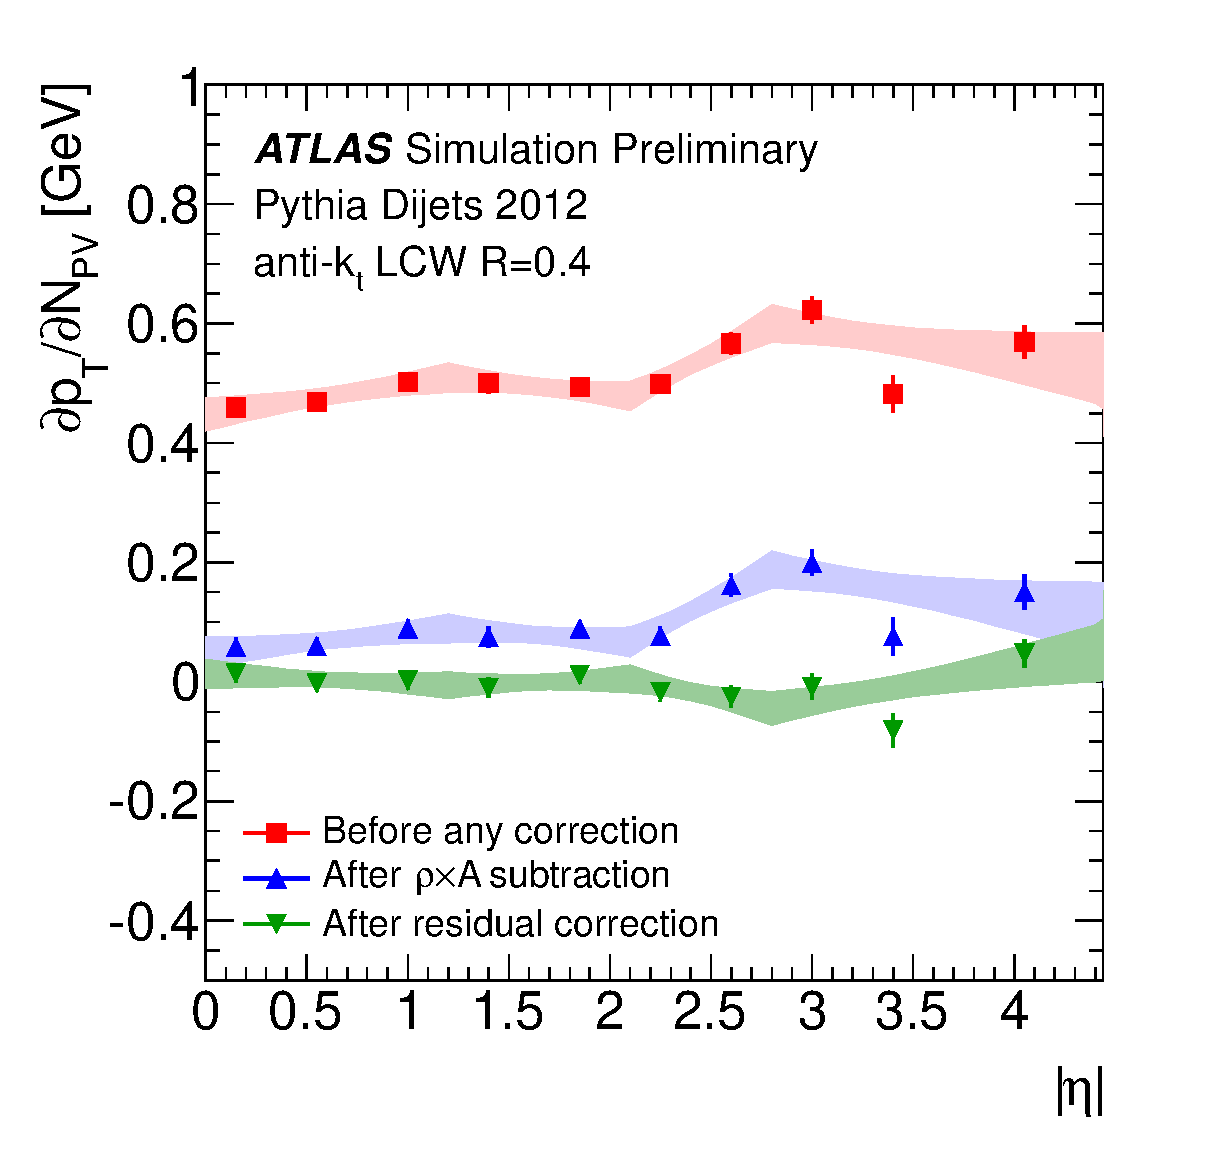
\includegraphics[width=0.495\textwidth]{ObjectReconstruction/Figures/JetPileupCorrNPV.eps}
      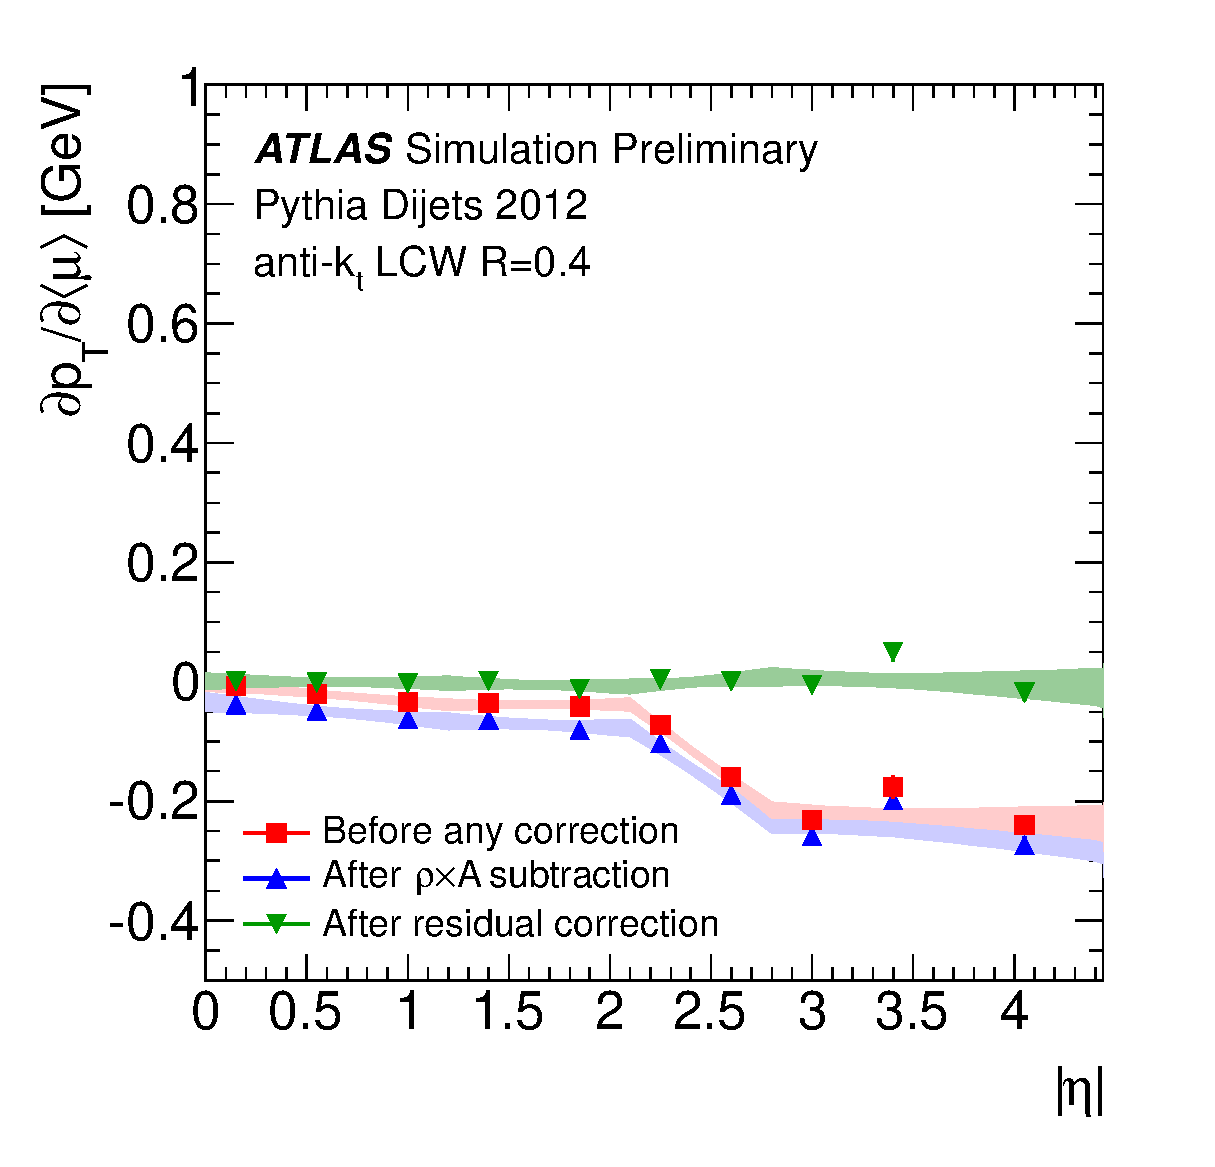
\includegraphics[width=0.495\textwidth]{ObjectReconstruction/Figures/JetPileupCorrMu.eps}
    }
  \end{center}
  \caption[Dependence of the reconstructed jet $\pt$ on in-time pileup and out-of-time pileup at various correction stages.]{Dependence of the reconstructed jet $\pt$ on in-time pileup (left) and out-of-time pileup (right) at various correction stages~\protect\cite{TheATLAScollaboration:2013pia}.}
  \label{fig:JetPileupCorrection}
\end{figure}

The fluctuations due to pileup effects in the energy of the jets with energies around the $\pt$ threshold or the reconstruction of jets coming from other pileup interactions, can increase the jet multiplicity of an event.
In order to reject these jets, information from the tracks associated to each jet is used.
The jet vertex fraction (JVF) is a variable aiming to identify the vertex from which a jet is originated. 
A schematic representation of the JVF principle is shown in Figure \ref{fig:JetPileup} (left).
It is calculated as the ratio of the sum of transverse momentum of matched tracks that originate from a chosen PV to the sum of transverse momentum of all matched tracks in the jet, independently of their origin. 
JVF is defined for each jet with respect to each PV, and therefore for a given jet $i$, its JVF with respect to the primary vertex $j$, PV$_j$, is given by:

\begin{equation}
\text{JVF}(\text{jet}_i, \text{PV}_j) = \frac{\sum_{k=1}^{N_\text{tracks}}{\pt(\text{track}_{k}^{\text{jet}_i}, \text{PV}_j) }}{ \sum_{n=1}^{N_\text{PV}}{\sum_{l=1}^{N_\text{tracks}}{\pt(\text{track}_{l}^{\text{jet}_i}, \text{PV}_n)} }}.
\label{eq:JetJVFDefinition}
\end{equation}

For the analysis presented in this thesis, the JVF will be defined with respect to the event hard-scatter vertex, which is selected as the primary vertex with the highest $\sum_{\text{tracks}}{(\pt^2)}$.

Figure \ref{fig:JetPileup} (right) shows the JVF distribution for hard-scatter jets and for pileup jets with $\pt^{\text{jet}}>\unit[20]{GeV}$ after the pileup subtraction, in order to illustrate the discriminating power of the JVF variable.
JVF values between 0 and 1 indicate the fraction of the $\pt$ of the associated tracks that come from the hard scattering.
If instead, no associated tracks are present, the JVF is set to -1.

\begin{figure}[!ht]
  \begin{center}
    \mbox{
      \includegraphics[width=0.495\textwidth]{ObjectReconstruction/Figures/JetJVFSchema.eps}
      \includegraphics[width=0.495\textwidth]{ObjectReconstruction/Figures/JetJVFDiscriminating.eps}
    }
  \end{center}
  \caption[Schematic representation of the JVF principle, and JVF distribution for hard-scatter jets and for pileup jets after the pileup subtraction.]{Schematic representation of the JVF principle (left). 
  JVF distribution for hard-scatter jets and for pileup jets with $\pt^{\text{jet}}>\unit[20]{GeV}$ after the pileup subtraction~\protect\cite{TheATLAScollaboration:2013pia} (right).}
  \label{fig:JetPileup}
\end{figure}


\subsubsection{Jet energy calibration}
    \label{subsubsec:JetEnergyCalibration}

The jet energy calibration restores the reconstructed jet energy to the energy of the Monte Carlo particle-level jets (truth jets).
It corrects for detector effects due to the mis-measurement of the energy deposited by hadrons in the calorimeter, the energy lost in inactive regions of the detector or the energy deposits of particles inside the particle-level jet entering the detector that are not included in the reconstructed jet.
The jet energy calibration can be applied to jets formed from topo-clusters at EM or LCW scale, the resulting being referred as EM+JES or LCW+JES jets, respectively.

To derive this calibration, all the isolated calorimeter jets that have a matching isolated particle-level jet at $\Delta R=0.3$ are considered.
An isolated jet is defined as having no other jet with $\pt>\unit[7]{GeV}$ within $\Delta R = 2.5 R$, being $R$ the distance parameter of the jet algorithm~\cite{Aad:2011he}.
The derivation of the jet energy response correction proceeds in several steps:

\begin{itemize}

\item The jet energy response,
    \begin{equation}
    \mathfrak{R}_{\text{jet}}^{\text{EM(LCW)}} = \frac{E_{\text{jet}}^{\text{EM(LCW)}}}{E_{\text{jet}}^{\text{truth}}},
    \label{eq:JetEnergyResponse}
    \end{equation}
    is computed for each pair of calorimeter and particle-level jets, measured in bins of truth jet energy, $E_{\text{jet}}^{\text{truth}}$ and calorimeter jet detector pseudorapidity\footnote{The detector $\eta$ is used instead of the origin corrected, used in physics analysis, because it more directly corresponds to a region of the calorimeter.}.

\item The averaged jet energy response, $\langle \mathfrak{R}_{\text{jet}}^{\text{EM(LCW)}} \rangle$, and the averaged reconstructed jet energy, $\langle E_{\text{jet}}^{\text{EM(LCW)}} \rangle$, are calculated for each $(E_{\text{jet}}^{\text{truth}}, $\eta$)$-bin.
These quantities are defined as the peak position of a Gaussian fit to the $\mathfrak{R}_{\text{jet}}^{\text{EM(LCW)}}$ and $E_{\text{jet}}^{\text{EM(LCW)}}$ distributions, respectively.
Figure \ref{fig:JetCalibrationResponse} (left) shows the averaged jet calibration response for the EM+JES scale, for various jet energies as a function of the jet $\eta$.
The values for the jet response vary between 0.85 and 0.55, increasing as the energy of the jet becomes larger and decreasing in the $\eta$ regions corresponding to the inactive regions of the calorimeters.


\item For each $\eta$ bin, the jet response calibration function, $\mathcal{F}_{\text{calib}}(E_{\text{jet}}^{\text{EM(LCW)}})$, is obtained by fitting the $(\langle E_{\text{jet}}^{\text{EM(LCW)}} \rangle, \langle \mathfrak{R}_{\text{jet}}^{\text{EM(LCW)}} \rangle)$ values corresponding to each $E_{\text{jet}}^{\text{truth}}$ bin.
The fitting function can be parametrized as:
    \begin{equation}
    \mathcal{F}_{\text{calib}}(E_{\text{jet}}^{\text{EM(LCW)}}) = \sum_{i=0}^{N_{\text{max}}}{a_i\left(\ln{E_{\text{jet}}^{\text{EM(LCW)}}}\right)^i},
    \label{eq:JetResponseFunction}
    \end{equation}
\noindent where $a_i$ are free parameters and $N_\text{max}$ is chosen between 1 and 6 depending on the goodness of the fit.

\end{itemize}

\begin{figure}[!ht]
  \begin{center}
    \mbox{
      \includegraphics[width=0.495\textwidth]{ObjectReconstruction/Figures/JetCalibrationResponse.eps}
      \includegraphics[width=0.495\textwidth]{ObjectReconstruction/Figures/JetCalibfig_EMJES_vs_pT_AntiKt6.eps}
    }
  \end{center}
  \caption[Average energy of jets formed from topoclusters calibrated at EM scale, and average jet energy scale correction as a function of the calibrated jet transverse momentum.]{Left: average energy of jets formed from topoclusters calibrated at EM scale with respect to the particle-level jet energy ($E_{\text{jet}}^{\text{EM}}/E_{\text{jet}}^{\text{truth}}$) as a function of the jet pseudorapidity before applying the correction for the event vertex shown separately for various jet energies \protect\cite{Aad:2011he}.
  Right: Average jet energy scale correction as a function of the calibrated jet transverse momentum for three representative $\eta^{\text{jet}}$-intervals obtained from the nominal MC simulation sample~\protect\cite{Aad:2011he}.
  }
  \label{fig:JetCalibrationResponse}
\end{figure}

The final jet energy scale correction that relates the measured calorimeter jet to the true jet energy is defined as $1/\mathcal{F}_{\text{calib}}(E_{\text{jet}}^{\text{EM(LCW)}})$, such that:

\begin{equation}
E_{\text{jet}}^{\text{EM+JES(LCW+JES)}} = \frac{E_{\text{jet}}^{\text{EM(LCW)}}}{\mathcal{F}_{\text{calib}}(E_{\text{jet}}^{\text{EM(LCW)}})|_{\eta}}.
\label{eq:JetJESCorrection}
\end{equation}

Figure \ref{fig:JetCalibrationResponse} (right) shows the jet energy scale correction as a function of the calibrated jet transverse momentum for three different $\eta$-intervals.
The values of the jet energy correction factors range from about 2.1 at low jet energies in the central region to less than 1.2 for high energy jets in the most forward region.


\subsubsection{Jet residual calibration}
    \label{subsubsec:JetResidualCalibration}

In the jet residual calibration, the data-to-MC differences are assessed using \emph{in-situ} techniques, which exploit the transverse momentum balance between a jet and well-measured photons, $Z$ bosons or jets.
This calibration is only applied to data, since it aims to restore the energy of the jets reconstructed in data to that from the Monte Carlo simulation\footnote{The reconstructed jets from the MC simulations are calibrated with the EM+JES or the LCW+JES scheme, which restores the reconstructed jet energy to that of the particle-level jet in the simulation, as shown in Section~\ref{subsubsec:JetEnergyCalibration}.}.
The jet energy once the residual calibration has been applied, $E_{\text{jet}}^{\text{data, in-situ}}$, is found to be:

\begin{equation}
E_{\text{jet}}^{\text{data, in-situ}} = \frac{E_{\text{jet}}^{\text{data}}}{\mathcal{C}(\pt^{\text{jet}}, \eta)},
\label{eq:JetInSituCorrection}
\end{equation}

\noindent where  $1 / \mathcal{C}(\pt^{\text{jet}}, \eta)$, the correction extracted from the jet in-situ calibrations, is defined as:

\begin{equation}
\mathcal{C}(\pt^{\text{jet}}, \eta) = \frac{\langle \pt^{\text{jet}} / \pt^{\text{ref}} \rangle_{\text{data}}}{\langle \pt^{\text{jet}} / \pt^{\text{ref}} \rangle_{\text{MC}}}\Bigg|_{\eta},
\label{eq:JetInSituCorrectionFactor}
\end{equation}

\noindent with $\langle \pt^{\text{jet}} / \pt^{\text{ref}} \rangle_{\text{data}}$ and $\langle \pt^{\text{jet}} / \pt^{\text{ref}} \rangle_{\text{MC}}$ being the ratio of the average jet response, measured in data and in the Monte Carlo simulation, respectively.

The residual jet calibration is computed following different strategies depending on whether the jet is contained in the central or in the forward regions of the detector.

In the central rapidity region, $|\eta_\text{det}|<1.2$, the jet energy can be calibrated as follows:

\begin{enumerate}
\item{\textbf{Jet energy calibration using $Z$-jet events: }}In events where one $Z$ boson is produced in association to only one jet, the jet recoils against the $Z$ boson ensuring approximate momentum balance between them in the transverse plane.
Ideally, the response of the jet in the calorimeters could be determined by using the $\pt$ of the $Z$ boson as the reference particle-level jet $\pt$.
However, uncertainties on the $Z$ boson decay products measurement, particles not included in the cone of the jet, additional parton radiation contributing to the recoil against the $Z$ boson or contributions from the underlying event prevent to use the measurement of $\langle\pt^{\text{jet}}/\pt^{\text{ref}}\rangle$ to estimate the jet response, but only to assess how well the MC simulation can reproduce the data.
Figure~\ref{fig:JetInSituMeasurements} (left) shows the mean $\pt$ balance measured in data and in a \pythia{} MC simulation, for EM+JES calibrated $\akt$ jets.
The $\pt$ balance, $\langle \pt^{\text{jet}} / \pt^{\text{ref}} \rangle$, ranges between 0.7 and 1 both in data and in the simulation, and it increases as the $\pt$ of the jet increases.
This figure also shows that the $\pt$ balance measured in the MC simulation is slightly higher compared to the measurement in data.
The advantage of the jet calibration using $Z$-jet events is the possibility of probing low-$\pt$ jets, which are difficult to reach with $\gamma$-jet events due to trigger thresholds and background contamination in that region.

\item{\textbf{Jet energy calibration using $\gamma$-jet events: }}The $\gamma$-jet events benefit from larger statistics for $\pt$ above 150~GeV compared to the $Z$-jet events.
Two in-situ techniques are used to probe the calorimeter response to jets recoiling the photons, for data and MC simulations.
On one hand, a technique based on the procedure used to determine the jet energy calibration using $Z$-jet events is followed, in which the highest $\pt$ jet is compared to the transverse momentum of the reference photon.
Alternatively, the missing transverse momentum projection fraction (MPF) technique \cite{Aad:2014bia} is used, in which the photon transverse momentum is balanced against the full hadronic recoil.

\item{\textbf{High-$\pt$ jet energy calibration: }}This technique is relevant for very high $\pt$ jets (at the TeV regime), where the calibrations extracted using the $Z$-jet and the $\gamma$-jet methods described above, are affected by statistical fluctuations.
Jets at very high $\pt$ are balanced against a recoil system of low $\pt$ jets, previously well calibrated using the $\gamma$-jet or the $Z$-jet balance.
\end{enumerate}

The final in-situ calibration obtained from the combination of these techniques is shown in Figure~\ref{fig:JetInSituMeasurements} (right), together with statistical uncertainties.
A general offset of about $-2\%$ is observed in the data-to-MC response ratios for jet transverse momenta below $\unit[100]{GeV}$.
The offset decreases to $-1\%$ at higher $\pt$ ($\pt \gtrsim \unit[200]{GeV}$).

\begin{figure}[!ht]
  \begin{center}
    \mbox{
      \includegraphics[width=0.495\textwidth]{ObjectReconstruction/Figures/Zjetfigures_balanceComparison_Jes_Akt4.pdf}
      \includegraphics[width=0.495\textwidth]{ObjectReconstruction/Figures/responseRatioSmooth_TSpline2_EMJES_R4.pdf}
    }
  \end{center}
  \caption[Mean $\pt$ balance obtained in the data and with the \pythia{} simulation, and ratio of the average jet response measured in data to that measured in MC simulations.]{Mean $\pt$ balance obtained in the data and with the \pythia{} simulation, for $\akt$ jets with $R=0.4$ calibrated with the EM+JES scheme (left)~\cite{Aad:2014bia}. Ratio of the average jet response $\langle \pt^{\text{jet}} / \pt^{\text{ref}} \rangle$ measured in data to that measured in MC simulations for jets within $|\eta|<1.2$ as a function of the jet transverse momentum, $\pt^{\text{jet}}$, shown separately for the three in-situ techniques, used in the combined calibration (right)~\cite{Aad:2014bia}.}
  \label{fig:JetInSituMeasurements}
\end{figure}

In the forward rapidity region, $|\eta_\text{det}|>1.2$, the calibration can be performed by exploiting the transverse momentum balance in events with two jets at high transverse momentum. 
A jet in the forward region can be balanced against a well-calibrated jet in the central region, and therefore, the whole detector response can be equalized as a function of $\eta^{\text{jet}}$.
In addition to this simple approach, the matrix method described in Ref.~\cite{ATLAS:2011jea} is used, in which the $\eta$-intercalibration is estimated from jets in all regions (not only the central one).


\section{Missing transverse energy}
    \label{subsec:ETmissReco}

The missing transverse momentum, $\ptmiss$, is defined as the momentum imbalance in the plane transverse to the beam axis.
The vector momentum imbalance in the transverse plane is obtained from the negative vector sum of the momenta of all particles detected in a $\pp$ collision.
The $\ptmiss$ reconstruction includes contributions from energy deposits in the calorimeters and muons reconstructed in the muon spectrometer \cite{TheATLAScollaboration:2013oia}.
The two $\ptmiss$ components are calculated as:

\begin{equation}
p_{x(y)}^{\text{miss}} = p_{x(y)}^{\text{miss,calo}} + p_{x(y)}^{\text{miss},\mu}.
\label{eq:ETmissDef_All}
\end{equation}

The magnitude of this vector is the so-called missing transverse energy, $\met$.
The values of $\met$ and its azimutal coordinate $\phi^\text{miss}$ are defined as:

\begin{equation}
\begin{split}
\met = \sqrt{(p_{x}^{\text{miss}})^2 + (p_{y}^{\text{miss}})^2},\\
\phi^{\text{miss}} = \arctan{(p_{y}^{\text{miss}} / p_{x}^{\text{miss}})}.
\end{split}
\label{eq:ETmissDef_pol}
\end{equation}

The reconstruction of the calorimeter term of the $\ptmiss$ uses calorimeter cells calibrated according to the reconstructed high-$\pt$ physics object to which they are associated, in a chosen order: electrons, photons, hadronically decaying $\tau$-leptons, jets and muons.
Cells not associated with any such objects are also taken into account in the $\met$ calculation.
Once the cells are associated with objects as described above, the $\ptmiss$ calorimeter term is calculated as follows \cite{Aad:1379858} (the reason why the $p_{x(y)}^{\text{miss,calo},\mu}$ term is in between parenthesis will become clear below):

\begin{equation}
\begin{split}
p_{x(y)}^{\text{miss,calo}} = p_{x(y)}^{\text{miss},e} + p_{x(y)}^{\text{miss},\gamma} + p_{x(y)}^{\text{miss},\tau} + p_{x(y)}^{\text{miss,jets}} \\
    p_{x(y)}^{\text{miss,softjets}} + (p_{x(y)}^{\text{miss,calo},\mu}) + p_{x(y)}^{\text{miss,CellOut}}.
\end{split}
\label{eq:ETmissDef_Calo}
\end{equation}

Each of the terms in the previous equation is computed from the negative sum of calibrated cell energies inside the corresponding object, according to the following expression:

\begin{equation}
\begin{split}
p_{x}^{\text{miss,term}} = \sum_{i=1}^{N_{\text{cell}}^{\text{term}}}{p_i \sin{\theta_i}\cos{\phi_i}} \\
p_{y}^{\text{miss,term}} = \sum_{i=1}^{N_{\text{cell}}^{\text{term}}}{p_i \sin{\theta_i}\sin{\phi_i}}
\end{split}
\label{eq:ETmissDef_Split}
\end{equation}

\noindent where $p_i$, $\theta_i$ and $\phi_i$ are the energy, the polar angle and the azimutal angle respectively, and all the summations are performed on cells in the range $|\eta|<4.5$.

The different terms in Equation \ref{eq:ETmissDef_Calo} are described in the following:

\begin{itemize}

\item{$p_{x(y)}^{\text{miss},e}$ }is reconstructed from cells in clusters associated to electrons passing the ``medium'' identification criteria with $\pt>\unit[10]{GeV}$.

\item{$p_{x(y)}^{\text{miss},\gamma}$ }is also reconstructed from cells in clusters, associated with photons passing the ``tight'' identification criteria \cite{ATLAS:2012ana} with $\pt>\unit[10]{GeV}$ at the EM scale.

\item{$p_{x(y)}^{\text{miss},\tau}$ }is reconstructed from cluster cells associated to LCW calibrated $\tau$-jets reconstructed with the ``tight'' identification criteria \cite{TheATLAScollaboration:2013wha}, with $\pt>\unit[10]{GeV}$.

\item{$p_{x(y)}^{\text{miss,jets}}$ }is computed from cells in clusters associated to LCW calibrated jets with  $\pt>\unit[20]{GeV}$, reconstructed with the $\akt$ algorithm, and with the jet energy scale factor applied.

\item{$p_{x(y)}^{\text{miss,softjets}}$} is reconstructed from cells in clusters associated to LCW calibrated jets reconstructed with the $\akt$ algorithm (with $R=0.6$), with $\unit[7]{GeV}<\pt<\unit[20]{GeV}$.

\item{$p_{x(y)}^{\text{miss,calo},\mu}$} is the contribution originating from energy lost by muons in the calorimeter.
Its calibration will be discussed below.

\item{$p_{x(y)}^{\text{miss,CellOut}}$} is calculated from the cells in topoclusters with the LCW calibration and from reconstructed tracks with $\pt>\unit[400]{MeV}$  which are not included in the reconstructed objects.
 The tracks are added to recover the contribution from low-$\pt$ particles which do not reach the calorimeter or do not have enough energy to seed a topocluster.
They are also used to improve the determination of the momentum in the topoclusters, since the calibration and resolution of the low $\pt$ tracks is better compared to that of the topoclusters.

\end{itemize}

On the other hand, the $\ptmiss$ muon term (see Equation \ref{eq:ETmissDef_All}) from the momentum of muon tracks reconstructed with $|\eta|<2.7$:

\begin{equation}
p_{x(y)}^{\text{miss},\mu} = - \sum_{\text{muons}}{p_{x(y)}}^{\mu},
\label{eq:ETmissDef_Mu}
\end{equation}

\noindent where the summation effects all the selected muons.
In the central region, $|\eta|<2.5$, combined muons (reconstructed muons in the MS with a matched track in the ID, see Section \ref{sec:MuonReco}) are considered.
Instead, since the region $2.5<|\eta|<2.7$ lays outside the fiducial volume of the ID, there is no matched track requirement and the MS $\pt$ alone is used.

The muon term is calculated differently for isolated and non-isolated muons, where non-isolated muons are defined to be those within a distance $\Delta R < 0.3$ of a reconstructed jet in the event.
For isolated muons, the $\pt$ is determined from the combined measurement in the ID and MS, accounting for the energy that the muon deposits in the calorimeter.
Therefore, $p_{x(y)}^{\text{miss,calo},\mu}$ is not added to the calorimeter contribution (this is the reason why it appears in between parenthesis in Equation \ref{eq:ETmissDef_Calo}).
Instead, for non-isolated muons, the term $p_{x(y)}^{\text{miss,calo},\mu}$ has to be considered.

The systematic uncertainty on each individual term of the $\met$ can be evaluated from the propagation of the uncertainties of the reconstructed objects that are used to build it.
Only the contribution to the $\met$ scale and resolution uncertainties coming from the ``soft terms'' (softjets and CellOut terms) needs to be estimated with dedicated studies \cite{TheATLAScollaboration:2013oia}.
The overall systematic uncertainty on the $\met$ scale is then calculated by combining the uncertainties on each term.

As it will be discussed in Section~\ref{sec:ObjectDefinition}, a slightly modified definition of the $\met$ is used\footnote{The $\met$ collection in the analysis presented is called ``\texttt{MET\_Egamma10NoTau}''.} in the analysis presented in this Thesis.
The $\tau$-lepton term, $p_{x(y)}^{\text{miss},\tau}$, is omitted because in the analysis presented, $\tau$-leptons are not identified as such, but considered as jets.
Furthermore, the muon terms, $p_{x(y)}^{\text{miss,calo},\mu}$ and $p_{x(y)}^{\text{miss},\mu}$, are also omitted.
The reason for not considering them is related to the precise estimation of the most important irreducible background in the analysis, $\znn$, which will be explained in Chapter~\ref{chapter:MonojetAnalysis}.

\cleardoublepage

\chapter{The monojet analysis}
    \label{chapter:MonojetAnalysis}

The monojet analysis is described in detail in this chapter.
The data and the Monte Carlo simulated samples used for the analysis are presented, together with the definition of the different physics objects and the event selection criteria.
The statistical treatment of the data and the estimation of the different Standard Model (SM) background processes are discussed.
The observations are then compared to the SM predictions in the different signal regions.


\section{Data sample}
    \label{sec:DataSample}

The data sample considered in the analysis presented in this Thesis was collected with the ATLAS detector in proton-proton collisions at a center of mass energy of $\unit[8]{TeV}$ between April 4, 2012 and December 6, 2012.
A total integrated luminosity of  $\unit[20.3 \pm 0.6]{fb^{-1}}$ was recorded after requiring tracking detectors, calorimeters, muon chambers and magnets to be fully operational during the data taking.
Events are selected using the lowest unprescaled $\met$ trigger logic called \texttt{EF\_xe80\_tclcw}, that selects events with $\met$ above $\unit[80]{GeV}$, as computed at the final stage of the three-level trigger system of ATLAS discussed in Section~\ref{subsec:TriggerSystem}. 
The details of the implementation of the $\met$ trigger can be found in Ref.~\cite{Casadei:2011via}.


\section{Object definition}
    \label{sec:ObjectDefinition}

Jets and $\met$ are used to define the signal selections whereas leptons are used to both veto the electroweak backgrounds and to define the different control samples.


\subsection{Jets}
    \label{subsec:JetDefinition}

Jets are reconstructed from energy deposits in the calorimeters using the $\akt$ jet algorithm with the jet radius parameter $R=0.4$ (see Section \ref{sec:JetReco}).
The transverse momentum of the jets is corrected for detector effects with the LCW calibration.
Jets with corrected $\pt>\unit[20]{GeV}$ and $|\eta|<2.8$ are considered in the analysis.
In order to remove jets originating from pileup collisions, central jets ($|\eta|<2.4$) with $\pt < \unit[50]{GeV}$ are required to have a jet vertex fraction (JVF) above 0.5.


\subsection{Electrons}
    \label{subsec:ElectronDefinition}

Electrons are required to have $\pt>\unit[20]{GeV}$ and $|\eta|<2.47$, and need to fulfill the \emph{medium} shower shape and track selection criteria (see Section \ref{sec:ElectronReco}).
The same $\pt$ threshold is used to veto electrons in the signal selections and to select them in the control samples (see Section~\ref{sec:EventSelection}), which minimizes the impact of the reconstruction, identification and efficiency systematic uncertainties.
The threshold of $\unit[20]{GeV}$ used in this definition combined to the definition of the electron control sample, brings the background of jets misidentified as electrons to negligible levels, and therefore no isolation is required.

Overlaps between identified electrons and jets in the final state are resolved.
Jets are discarded if their separation $\Delta R$ from an identified electron is less than 0.2.
The electrons separated by $\Delta R$ between 0.2 and 0.4 from any remaining jet are removed.


\subsection{Muons}
    \label{subsec:MuonDefinition}

Muons are reconstructed by combining information from the muon spectrometer and inner tracking detectors (see Section~\ref{sec:MuonReco}).
The muon candidates for the analysis presented are required to have $\pt>\unit[10]{GeV}$, $|\eta|<2.4$, and $\Delta R > 0.4$ with respect to any jet candidate with $\pt > \unit[30]{GeV}$.
The use of this $\pt$ threshold increases the precision for selecting real muons from $W$ boson decays, and avoids the bias in the muon selection due to the presence of low $\pt$ jets with large pileup contributions.
Finally, an isolation condition is applied to the muons, that requires the sum of the $\pt$ of the tracks not associated with the muon in a cone of radius $\Delta R = 0.2$ around the muon direction, to be less than $\unit[1.8]{GeV}$.

\subsection{Missing transverse energy}
    \label{subsec:MetDefinition}

The missing transverse energy is described in detail in Section~\ref{subsec:ETmissReco}.
It is reconstructed using all energy deposits in the calorimeter up to a pseudorapidity $|\eta|<4.9$, and without including information from identified muons in the final state.


\section{Event selection}
    \label{sec:EventSelection}

The different signal regions defined in this analysis have a common preselection criteria, that suppresses large contribution of SM processes with leptons in the final state and non-collision background contributions:

\begin{itemize}
\item Events are required to have a reconstructed primary vertex consistent with the beam spot envelope and it is required to have at least five isolated tracks with $\pt>\unit[400]{MeV}$.
If two or more vertices are consistent with these requirements, the one with the largest sum $\pt^2$ is chosen as primary vertex.
This requirement removes beam-related backgrounds and cosmic rays.

\item Events are initially requested to have $\met>\unit[150]{GeV}$ in order to ensure the trigger to be fully efficient.

\item At least one jet with $\pt>\unit[150]{GeV}$ and $|\eta|<2.8$ is required in the final state, in order to select monojet-like configurations.

\item Different quality cuts are applied to remove events recorded during a LAr noise burst or during a failure in the electronics of any subsystem.
Also events not correctly processed are vetoed from the selection.

\item Events containing any jet with $\pt>\unit[20]{GeV}$ and $|\eta|<4.5$ with charged fraction \footnote{The charged fraction is defined as $f_{\text{ch}} = \sum{\pt^{\text{track,jet}}/\pt^{\text{jet}}}$, where $\sum{\pt^{\text{track,jet}}}$ is the scalar sum of the transverse momenta of the tracks associated to the primary vertex within a cone of radius 0.4 around the jet axis, and $\pt^{\text{jet}}$ is the transverse momentum as determined from the calorimetric measurements.}, 
electromagnetic fraction\footnote{The electromagnetic fraction is defined as $f_{\text{em}} = E_{\text{LAr}}/(E_{\text{LAr}} + E_{\text{TileCal}})$, where $E_{\text{LAr}}$ is the energy deposited in the electromagnetic calorimeter and $E_{\text{TileCal}}$ is the energy deposited in the hadronic calorimeter.} 
or sampling fraction\footnote{$f_{\text{max}}$ denotes the maximum fraction of the jet energy collected by a single calorimeter layer.} inconsistent with the requirement that they originate from a $\pp$ collision ($f_{\text{ch}}<0.02$, $f_{\text{em}}<0.1$ and $f_{\text{max}}>0.8$ respectively), are vetoed.

\item Events with one or more reconstructed isolated muons with $\pt>\unit[10]{GeV}$ or electrons with $\pt>\unit[20]{GeV}$ are vetoed.
\end{itemize}

A maximum of three jets with $\pt>\unit[30]{GeV}$ and $|\eta|<2.8$ in the event are allowed.
An additional requirement on the azimutal separation of $\Delta\phi(\text{jet}, \met) > 0.4$ between the missing transverse momentum direction and that of each of the selected jets is imposed.
The latest suppresses the multijet background contribution where the large $\met$ originates from a jet energy mismeasurement.

Three separate signal regions (denoted by M1, M2 and M3) are defined with increasing lower thresholds on the leading jet $\pt$ and $\met$.
The definition of these signal regions come as a result of an optimization on the stop pair production with $\stoptocharm$ model, performed across the stop-neutralino mass plane with increasing $\stopone$ and $\ninoone$ masses.

For the M1 selection, the events are required to have $\met>\unit[220]{GeV}$ and leading jet $\pt>\unit[280]{GeV}$. M2 (M3) selection must have $\met>\unit[340]{GeV}$ ($\met>\unit[450]{GeV}$) and leading jet $\pt>\unit[340]{GeV}$ ($\pt>\unit[450]{GeV}$).

Three extra generic signal regions (M4, M5 and M6) are defined to increase the sensitivity to a broad variety of models leading to final states with larger $\met$. Signal region M4 requires the events to have leading jet $\pt>\unit[450]{GeV}$ and $\met>\unit[340]{GeV}$, while region M5 (M6) are required to have leading jet $\pt>\unit[550]{GeV}$ and $\met>\unit[550]{GeV}$ (leading jet $\pt>\unit[600]{GeV}$ and $\met>\unit[600]{GeV}$).
Table \ref{tab:SignalRegionCuts} summarizes the six signal region selections.

\begin{table}[!ht]
  \renewcommand{\baselinestretch}{1}
  \begin{center}
    \begin{small}
      \begin{tabular*}{\textwidth}{@{\extracolsep{\fill}}lcccccc}\hline\hline
        \multicolumn{7}{c}{\small{\textbf{Selection criteria}}} \\\hline
        %%% --- PRESELECTION
        \multicolumn{7}{c}{{\small{Preselection}} } \\\hline
        \multicolumn{7}{l}{Primary vertex}\\
        \multicolumn{7}{l}{$\met > 150$~GeV }\\
        \multicolumn{7}{l}{At least one jet with $\pt >150$~GeV and $|\eta|< 2.8$}\\
        \multicolumn{7}{l}{Jet quality requirements}   \\
        \multicolumn{7}{l}{Lepton vetoes}\\ \hline
        %%% --- MONOJET
        \multicolumn{7}{c}{\small{Monojet-like selection}}\\\hline
        \multicolumn{7}{l}{At most a total of three jets with $\pt > 30$~GeV and $|\eta|<2.8$}\\
        \multicolumn{7}{l}{$\Delta\phi(\text{jet}, \met) > 0.4$} \\\hline
        Signal region                   & M1  & M2  & M3  & M4  & M5  & M6  \\
        Minimum leading jet $\pt$ [GeV] & 280 & 340 & 450 & 450 & 550 & 600 \\
        Minimum $\met$ [GeV]            & 220 & 340 & 450 & 340 & 550 & 600 \\ \hline\hline
      \end{tabular*}
    \end{small}
  \end{center}
  \caption{Event selection criteria applied for the signal regions M1 to M6.}
  \label{tab:SignalRegionCuts}
\end{table}


\section{Monte Carlo simulated samples}
    \label{sec:MCSamples}

The analysis uses MC samples to estimate each Standard Model process.
The MC events are passed through a detailed simulation of the detector based on {\sc Geant4} \cite{Agostinelli:2002hh}.
Different in-time and out-of-time pileup conditions as a function of the instantaneous luminosity are also taken into account by overlaying simulated minimum-bias events generated with \pythia-8 onto the hard scattering process and re-weighting them with the distribution of the observed mean number of interactions per bunch crossing.

In the following, details are given for the SM background MC simulated samples.


\subsection{$W$+jets and $Z$+jets}
    \label{subsec:WZjetsMCSimulation}

A set of simulated $W$+jets and $Z$+jets events are generated using \sherpa{}, including LO matrix elements for up to 5 partons in the final state and using massive $b/c$-quarks, CT10 parton distribution functions\footnote{Next-to-next-to-leading order (NNLO) PDFs from the CTEQ/TEA group.} and its own model of hadronization.
Similar samples have been generated with the \alpgen{} generator, to study the modeling uncertainties.
The MC samples are initially normalized to next-to-next-to-leading-order (NNLO) cross sections in perturbative QCD (pQCD) with the DYNNLO \cite{Catani:2007vq} program using MSTW2008 NNLO PDF sets.


\subsection{Top} 
    \label{subsec:TopSimulation}

The production of top quark pairs (\ttbar) is simulated using the \powheg{} MC generator.
A top quark mass of $\unit[172.5]{GeV}$, the CTEQ6L1 parton distribution functions and the Peruggia 2011C Tune \cite{Skands:2010ak} have been used for the generation and the underlying event simulation.
The $\ttbar$ samples are normalized to NNLO+NNLL (next-to-next-to-leading-logarithm pQCD accuracy), determined by \texttt{Top++2.0}.
Similar \alpgen{} and \mcnlo{} samples are used to assess the $\ttbar$ modeling uncertainties.

Single top samples are generated with \powheg{} for the $s$- and $Wt$-channels, while \acer{} \cite{Kersevan:2002dd} is used for the $t$-channel.
An approximate NLO+NNLL pQCD prediction is used for the $Wt$ process.
Samples generated with the \mcnlo{} generator are then used to estimate the systematic uncertainties.

\subsection{Diboson}
    \label{subsec:DibosonSimulation}

Diboson samples ($WW$, $WZ$ and $ZZ$ production) are generated with \sherpa{}, using massive $c$/$b$-quarks, with CT10 PDF and are normalized to NLO predictions.
Similar samples generated with \herwig{} are used to compute the modeling uncertainties.



\section{Background estimation}
    \label{sec:BkgEstimation}

The expected SM background is dominated by $\znn$ (irreducible), $\wln$ and $\ttbar$ production, and includes small contributions from $\zgammall$, single top, diboson and multijet processes.

The $W/Z$+jets backgrounds are estimated using MC event samples normalized using data in control regions.
The simulated $W/Z$+jets events are re-weighted to data as a function of the generated $\pt$ of the vector boson, which is found to improve the agreement between data and simulation.
The weights are extracted from the comparison of the reconstructed boson $\pt$ distribution in data and {\sherpa} MC simulation in a $W$+jets control sample where the jet and $\met$ preselection requirements from Table \ref{tab:SignalRegionCuts} have been applied.
As detailed in Appendix~\ref{app:BosonPtReweight}, these weights are defined in several bins in the boson $\pt$ and applied to the truth boson $\pt$ distribution of the simulated samples.
Due to the limited number of data events at large boson $\pt$, an inclusive last bin with boson $\pt > \unit[400]{GeV}$ is used.
The uncertainties of the re-weighting procedure are taken into account in the final result.

The top-quark background contribution is very small and is determined using MC simulated samples.
The simulated $\ttbar$ events are re-weighted based on the measurement in the data (as described in Ref.~\cite{Aad:2012hg}), indicating that the differential cross section as a function of the $\pt$ of the $\ttbar$ system is softer than that predicted by the MC simulation.
The diboson background contribution is also very small and fully determined using MC simulated samples.

The multijet background with large $\met$ originates mainly from the misreconstruction of the energy of a jet in the calorimeter, and to a lesser extent from the presence of neutrinos in the decays from heavy-flavor hadrons.
In this analysis the multijet background is estimated from data using the {\em jet smearing method}, which is described detail in Appendix~\ref{app:JetSmearingMethod}.
The jet smearing method relies on the assumption that the $\met$ of multijet events is dominated by fluctuations in the jet response in the detector that can be measured in the data.
The contribution of multijet processes is then normalized in regions defined with exactly the same requirements as the signal regions (Table \ref{tab:SignalRegionCuts}), but with the cut on the angular separation between the transverse momentum of the jets and the missing transverse energy, reverted ($\Delta\phi(\text{jet}, \met) < 0.4$).

The cleanup cuts applied to the data sample in Section~\ref{sec:EventSelection} are expected to maintain the non-collision contributions at a percent level.
The shape of the timing distribution for non-collision background events is reconstructed from a control data sample with relaxed jet cleanup cuts, and then extrapolated to the signal regions.
This extrapolation led to no events in the control samples after cuts, which is an indication that the level of non-collision background is negligible in the analysis.


\subsection{Definition of the $W/Z$+jets control regions}
    \label{subsec:ControlRegionsDefinition}

Control regions in data are defined for each signal selection, orthogonal to them, with identified electrons or muons in the final state and with the same requirements on the jet $\pt$, subleading jet vetoes and $\met$.
They are used to determine the $W/Z$+jets electroweak background contributions from data.

A $\wmn$+jets control sample is defined using events with a muon with $\pt>\unit[10]{GeV}$ and $W$ transverse mass, $\mt$, in the range $\unit[30]{GeV} < \mt < \unit[100]{GeV}$ to further enhance the $\wmn$+jets process.
The transverse mass is defined by the lepton ($\ell$) and neutrino ($\nu$) transverse momenta and their $\phi$-directions as:

\begin{equation}
\mt = \sqrt{ 2\pt^{\ell}\pt^{\nu}(1-\cos{(\phi^{\ell}-\phi^{\nu})}},
\label{eq:TransverseMassDef}
\end{equation}

\noindent where the ($x, y$) components of the neutrino momentum are taken to be the same as the corresponding $\ptmiss$ components.
Similarly, a $Z/\gamma^{\ast}(\rightarrow \mu^{+}\mu^{-})$+jets control sample is defined using events with exactly two muons with invariant mass range $\unit[66]{GeV}<m_{\mu\mu}<\unit[116]{GeV}$, i.e. around the peak of the $Z$ boson resonance.
Finally, a $\wen$+jets dominated control sample is also defined for each signal selection with an electron candidate with $\pt>\unit[20]{GeV}$.
Figure~\ref{fig:Plot_M1_CR_beforeFit} shows the $\met$ and the leading jet $\pt$ distributions for the three control regions described above for the selection cuts M1.


\begin{figure}[!ht]
  \begin{center}
    \mbox{
      \includegraphics[width=0.495\textwidth]{MonojetAnalysis/Figures/plot_Stop_A6_CRele_met.eps}
      \includegraphics[width=0.495\textwidth]{MonojetAnalysis/Figures/plot_Stop_A6_CRele_pt1.eps}
    }
    \mbox{
      \includegraphics[width=0.495\textwidth]{MonojetAnalysis/Figures/plot_Stop_A6_CRwmn_met.eps}
      \includegraphics[width=0.495\textwidth]{MonojetAnalysis/Figures/plot_Stop_A6_CRwmn_pt1.eps}
    }
    \mbox{
      \includegraphics[width=0.495\textwidth]{MonojetAnalysis/Figures/plot_Stop_A6_CRzmm_met.eps}
      \includegraphics[width=0.495\textwidth]{MonojetAnalysis/Figures/plot_Stop_A6_CRzmm_pt1.eps}
    }
  \end{center}
  \caption[$\met$ and leading jet $\pt$ distributions in the three control region for the selection cuts of region M1 compared to the background predictions.]{$\met$ and leading jet $\pt$ distributions in the three control region for the selection cuts of region M1 compared to the background predictions. The error bands in the ratios include the statistical and experimental uncertainties on the background predictions.}
  \label{fig:Plot_M1_CR_beforeFit}
\end{figure}

Monte Carlo-based normalization factors, determined from the \sherpa{} simulation and including the boson $\pt$ re-weighting explained above, are defined for each of the signal selections to estimate the different electroweak background contributions in the signal regions.
As an illustrative example, the contribution from the dominant $\znn$ background process to a given signal region, $N^{Z(\rightarrow\nu\nu)}_{\text{signal}}$, would be determined using the $\wmn$+jets control sample in data, according to:

\begin{equation}
N^{Z(\rightarrow\nu\bar{\nu})}_{\text{signal}} = N^{\text{MC}(Z(\rightarrow\nu\bar{\nu}))}_{\text{signal}} \times
        \frac{\left(N^{\text{data}}_{W(\rightarrow\mu\nu),\text{control}} - N^{\text{non-}W}_{W(\rightarrow\mu\nu),\text{control}} \right)}{N^{\text{MC}}_{W(\rightarrow\mu\nu),\text{control}}},
\label{eq:scaleFactorZnunu}
\end{equation}

\noindent where $N^{\text{MC}(Z(\rightarrow\nu\bar{\nu}))}_{\text{signal}}$ is the background predicted by the MC simulation in the signal region, and $N^{\text{data}}_{W(\rightarrow\mu\nu),\text{control}}$, $N^{\text{MC}}_{W(\rightarrow\mu\nu),\text{control}}$, and $N^{\text{non-}W}_{W(\rightarrow\mu\nu),\text{control}}$ denote, in the control region, the number of $\wmn$+jets candidates in data and MC simulation, and the non-$\wmn$ background contribution, respectively.
The latest term refers mainly to top-quark and diboson processes, but also includes contributions from other $W/Z$+jets processes.
The normalization factor for this particular example (e.g. the last factor from the previous expression), is defined as the ratio of the number of observed $\wmn$+jets events over the total number of $\wmn$+jets simulated events, both in the control region.


\section{Fit of the background processes to the data}
    \label{sec:Fit}

The use of control samples to constrain the dominant background contribution from $\znn$ and $W$+jets, reduces significantly the otherwise relatively large theoretical and experimental systematic uncertainties, of the order of 20\%--30\%, associated with purely MC-based background predictions in the signal regions.
For each selection and in order to both normalize and constrain the corresponding background estimates in the different signal regions, and to determine the final uncertainty in the total background, the likelihood shown in Equation~\ref{eq:PdfFit},

\begin{equation}
L(\vec{\mu}, \vec{\alpha}) = 
 \prod_{c \in \text{regions}}{\frac{[\nu_c(\vec{\mu}, \vec{\alpha})]^{n_c}}{n_c!}e^{-\nu_c(\vec{\mu}, \vec{\alpha})}},
 \prod_{p\in\text{params}}{P_p(\alpha_p)},
\label{eq:PdfFit_copy}
\end{equation}

\noindent is simultaneously fitted to the $W(\rightarrow \mu\nu)$+jets, $\zmm$+jets and $W(\rightarrow e\nu)$+jets control samples, taking into account the cross contamination between the different background sources in the control samples.


\subsection{Normalization factors}
    \label{subsec:FreeParameters}

The likelihood includes unconstrained normalization factors that can adjust the relative contributions of the main processes ($\vec{\mu}$ in Equation \ref{eq:PdfFit_copy}).
In particular, three normalization factors are considered, determined from the $\wmn$+jets, $\zmm$+jets and $\wen$+jets control regions, denoted as \texttt{mu\_Wmn}, \texttt{mu\_Zmm} and \texttt{mu\_Ele}.
The \texttt{mu\_Wmn} factor is used to constrain the normalization of the $\wmn$+jets and the $\znn$ processes.
The \texttt{mu\_Zmm} factor sets the normalization of the $\zmm$+jets process.
Finally, the \texttt{mu\_Ele} factor determines the normalization of the $\wen$+jets, $\wtn$, $\zee$+jets and $\ztt$+jets processes.
Table~\ref{tab:scaleFactorsSummary} shows a summary of the normalization factors used to normalize each background process.

\begin{table}[!ht]
  \begin{center}
    \begin{small}
      \begin{tabular}{lc}
      \hline\hline
        {\bf Process} & {\bf Normalization factor} \\
        \hline
        $\wen$+jets   & \texttt{mu\_Ele} \\ 
        $\wmn$+jets   & \texttt{mu\_Wmn} \\ 
        $\wtn$   & \texttt{mu\_Ele} \\ 
        $\znn$   & \texttt{mu\_Wmn} \\ 
        $\zee$+jets   & \texttt{mu\_Ele} \\ 
        $\zmm$+jets   & \texttt{mu\_Zmm} \\ 
        $\ztt$+jets   & \texttt{mu\_Ele} \\ 
        Top      & -- \\ 
        Dibosons & -- \\ 
        Multijet & -- \\ 
       \hline\hline
      \end{tabular}
    \end{small}
  \end{center}
  \caption{Summary of the normalization factors used to normalize the different background processes in the signal region.}
  \label{tab:scaleFactorsSummary}
\end{table}

The choice for the normalization factor \texttt{mu\_Wmn} instead of \texttt{mu\_Zmm}, to estimate the $\znn$ contribution, is motivated by the statistical power of the $\wmn$ control sample in data, about seven times larger than the $\zmm$+jets control sample.
Appendix~\ref{app:ClosureTestZnunu} provides Monte Carlo studies, both at particle and at detector level, that confirm the validity of the use of \texttt{mu\_Wmn} to normalize the $\znn$ process.


\subsection{Systematic uncertainties}
    \label{subsec:MonojetSystematicUncertainties}

The likelihood from Eq.~\ref{eq:PdfFit_copy} also includes nuisance parameters, $\vec{\alpha}$, that parametrize the contributions of the processes as a function of variations in fractions of sigma, with respect to their nominal prediction, for each systematic uncertainty.
These nuisance parameters are normally distributed, with mean 0, indicating that they are centered in the value corresponding to the nominal prediction, and standard deviation 1, in units of potential systematic variations.
In the global fit, each nuisance parameter is initialized at such values, and the fit is then allowed to profile the different systematic uncertainties in order to find the configuration that maximizes the likelihood.
Values for the nuisance parameters largely differing from 0 would indicate a large mismodeling, and that the fit tries to accommodate to the data with an anomalously large variation of systematic uncertainties.

The systematic uncertainties considered in this analysis are summarized and related to their corresponding nuisance parameters in Table~\ref{tab:monosyslist}.
A description of each systematic source is detailed below.
For each uncertainty, the impact on the total background yield before the fit\footnote{Therefore, the effect in the background contribution corresponding to $\alpha_\text{syst} = \pm 1$} is also discussed.
These values are included as inputs in the global analysis fit.
The systematic uncertainties are assumed to be correlated through the different background processes, and control and signal regions, unless the contrary is stated.

%--- \ref{tab:monosyslist}
\begin{table}
\begin{center}
\begin{scriptsize}
\begin{tabular}{|l|l|}
\hline
\multicolumn{2}{|c|}{{\bf Parameter definition}} \\ \hline
{\bf Free parameters} & {\bf Definition}            \\
\hline
\texttt{mu\_Ele}             & Normalization factor \\ 
\texttt{mu\_Wmn}             & Normalization factor \\ 
\texttt{mu\_Zmm}             & Normalization factor \\ \hline \hline
{\bf Nuisance parameters} & {\bf Definition}           \\ 
\texttt{alpha\_JES   }       & Uncertainty on the jet energy scale. \\ 
\texttt{alpha\_JER   }       & Uncertainty on the Jet energy resolution. \\ 
\texttt{alpha\_JvfUnc}       & Uncertainty due to the jet vertex fraction cut. \\ 
\texttt{alpha\_Pileup}       & Uncertainty on the pileup reweighing. \\ 
\multirow{2}{*}{\texttt{alpha\_SCALEST}}      & Uncertainty on the cell out energy scale of the missing transverse \\
                    & energy. \\ 
\multirow{2}{*}{\texttt{alpha\_RESOST}}       & Uncertainty on the cell out energy resolution of the missing \\
                    & transverse energy. \\ 
\texttt{alpha\_EEFF  }       & Uncertainty on the identification efficiency of the electrons. \\ 
\texttt{alpha\_EGZEE }       & Uncertainty on the energy scale of the electrons (Z scale). \\ 
\texttt{alpha\_EGMAT }       & Uncertainty on the energy scale of the electrons (material). \\ 
\texttt{alpha\_EGLOW }       & Uncertainty on the energy scale of the electrons (low momentum). \\ 
\texttt{alpha\_EGPS  }       & Uncertainty on the energy scale of the electrons (presampler). \\ 
\texttt{alpha\_EGRES }       & Uncertainty on the energy resolution of the electrons. \\ 
\texttt{alpha\_MEFF  }       & Uncertainty on the identification efficiency of the muons.\\ 
\texttt{alpha\_MSCALE}       & Uncertainty on the energy scale of the muons. \\ 
\multirow{2}{*}{\texttt{alpha\_MMS}}          & Uncertainty on the energy resolution of the muons (muon \\
                    & spectrometer). \\ 
\texttt{alpha\_MID         } & Uncertainty on the energy resolution of the muons (inner detector) \\ 
\texttt{alpha\_ktfac       } & Uncertainty on the factorization scale of the W/Z+jets. \\ 
\texttt{alpha\_qfac        } & Uncertainty on the matching scale of the W/Z+jets. \\ 
\texttt{alpha\_pdfUnc      } & Uncertainty on the PDFs of the $W/Z$+jets processes. \\ 
\multirow{2}{*}{\texttt{alpha\_bosonPtReweight}}& Uncertainty on the re-weighting of the $W/Z$+jets Sherpa samples, \\
                    & based on the truth boson $p_T$. \\ 
\multirow{3}{*}{\texttt{alpha\_WZtransfer}}   & Uncertainty on the $\znn$ estimation to cover for the \\
                    & differences on the MC modeling and EWK NLO corrections \\
                    & between $W$ and $Z$ processes. \\
\texttt{alpha\_ttbarGen    } & Uncertainty on the MC generator of the ttbar sample. \\ 
\texttt{alpha\_ttbarXsec   } & Uncertainty on the cross-section of the ttbar sample. \\ 
\texttt{alpha\_ttbarRad    } & Uncertainty on the ISR/FSR of the ttbar sample. \\ 
\texttt{alpha\_ttbarRen    } & Uncertainty on the renormalization scale of the ttbar sample. \\ 
\texttt{alpha\_ttbarFac    } & Uncertainty on the factorization scale of the ttbar sample. \\ 
\texttt{alpha\_ttbarPs     } & Uncertainty on the parton shower modelling of the ttbar sample. \\ 
\texttt{alpha\_singleTGen  } & Uncertainty on the MC generator of the single top sample. \\ 
\texttt{alpha\_singleTXsecS} & Uncertainty on the $s$-channel cross-section of the single top sample. \\ 
\texttt{alpha\_singleTXsecT} & Uncertainty on the $t$-channel cross-section of the single top sample. \\ 
\texttt{alpha\_singleTXsecW} & Uncertainty on the $Wt$ cross-section of the single top sample. \\ 
\texttt{alpha\_singleTRad  } & Uncertainty on the ISR/FSR of the single top sample. \\ 
\texttt{alpha\_singleTInt  } & Uncertainty on the interference with ttbar of the single top sample. \\ 
\multirow{2}{*}{\texttt{alpha\_singleTPs}}    & Uncertainty on the parton shower modelling for the $Wt$ channel \\
                    & of the single top sample. \\ 
\texttt{alpha\_dibRen      } & Uncertainty on the renormalization scale of the diboson sample.  \\ 
\texttt{alpha\_dibMatch    } & Uncertainty on the matching scale of the diboson sample. \\ 
\texttt{alpha\_dibFac      } & Uncertainty on the factorization scale of the diboson sample.  \\ 
\texttt{alpha\_dibXsec     } & Uncertainty on the cross-section of the diboson sample. \\ 
\multirow{2}{*}{\texttt{alpha\_qcdNorm}}      & Uncertainty on the normalization of the multi jet background \\
                    & estimation. \\
\texttt{alpha\_Luminosity  } & Uncertainty on the measurement of the luminosity in ATLAS. \\ \hline
\end{tabular}
\end{scriptsize}
\end{center}
\caption{List of all nuisance parameters used in the analysis and their definition in terms of
normalization factors and sources of systematic uncertainty.}
\label{tab:monosyslist}
\end{table} 


\paragraph{Jet Energy Scale:} The uncertainty on the absolute jet energy scale (JES) is one of the main uncertainties.
In the analysis it is parametrized by a single nuisance parameter, although is the result of combining 18 systematic sources\footnote{The performance of the fit has also been checked when 18 nuisance parameters are considered, and has lead to identical results.}, from the different steps of the jet energy scale calibration.
The effect of this uncertainty on the total MC prediction, before it is profiled in the global fit.
Before the fit it is approximately 7\% in both the signal and control regions.

\paragraph{Jet Energy Resolution:} The effect of the jet energy resolution (JER) in the total background yield is measured in each of the signal regions, and found to be less than 1\%.

\paragraph{Jet Vertex Fraction:} The effect of a possible mismodeling in the JVF distribution is investigated by studying the impact in the background yields when the requirement is varied from 0.5 to 0.47 and 0.53.
An effect below 1\% in the total background yield is found in all the signal regions.

\paragraph{Pile up:} The MC generated events need to be re-weighted in order to correctly describe the pileup conditions in the collisions.
This weights are extracted from the comparison of the number of interactions per bunch crossing distribution in both data and MC simulation.
Variations on these weights lead to negligible effects in the total background prediction.

\paragraph{$\met$ cell-out:}The resolution and scale uncertainties of the CellOut term of the $\met$ are also considered, and each of them is parametrized by a single nuisance parameter.
The effect of these uncertainties to the total background in the different signal regions is less than 1\%.

\paragraph{Leptons:} The uncertainty on the electron identification varies the total background yield in the signal regions by less than 1\%, and is parametrized by a single nuisance parameter.
The effect of the electron energy resolution, also parametrized by one nuisance parameter, leads to a negligible effect.
The uncertainty on the electron energy scale accounts for: the variations coming from the $Z$~scale uncertainty; the modeling of the interaction of the electrons with the calorimeter; the presampler scale uncertainty; and the scale uncertainty for low-$\pt$ electrons.
This is included in the fit via four separated nuisance parameters, which altogether introduce less than a 0.5\% variation in the total background yield.

The uncertainty on the muon identification translates into a 1\% variation on the total background in all the signal regions, and is parametrized by one nuisance parameter.
The uncertainty on the muon energy resolution accounts for the resolution effects coming from the Inner Detector and the Muon Spectrometer.
This uncertainty, parametrized with two different nuisance parameters, has a negligible effect on the total background contribution.
Finally, the uncertainty on the muon energy scale, affects the total background prediction in the signal regions by approximately 0.5\%, and is introduced in the global fit via one nuisance parameter.

\paragraph{Theoretical uncertainties on the $W/Z$+jets processes:}
Uncertainties on the factorization, renormalization, and parton-shower matching scales and PDFs of the $W/Z$+jets processes, are parametrized, each of them, by a different nuisance parameter.
Combined, they produce a variation between 20\% and 25\% in the total background yields, in the different signal selections.
An additional nuisance parameter is devoted to parametrize the uncertainty of the re-weighting of the boson $\pt$, and affects the total background prediction by a 2\%.
Finally, systematic uncertainties to account for the validity of the use of the $\wmn$+jets process to extract the normalization for $\znn$ and higher-order electroweak corrections affecting differently the $W$+jets and the $Z$+jets processes, are also considered~\cite{Denner:2009gj,Denner:2011vu,Denner:2012ts}.
These two effects are parametrized together by a single nuisance parameter, and modify the total background yield between 2\% and 4\% in the different signal regions.
More details on the estimation of this uncertainty can be found in Appendix~\ref{app:ClosureTestZnunu}.

\paragraph{Theoretical uncertainties on the top-quark-related processes:} Uncertainties on the absolute $\ttbar$ and single top cross sections; uncertainties on the MC generators and the modeling of parton showers employed; variations in the set of parameters that govern the parton showers and the amount of initial- and final-state soft gluon radiation; and uncertainties due to the choice of renormalization and factorization scales and PDFs are considered.
The effect of these systematic uncertainties on the total background prediction, varies between 1.6\% and 1.0\% for the different signal selections, and are represented by 13 different nuisance parameters in the fit.

\paragraph{Theoretical uncertainties on the diboson:} These uncertainties are estimated in a similar way as for the top-quark-related processes, and translate to an effect on the total background between 0.7\% and 2.3\%.
In the fit, these uncertainties are parametrized by 4 nuisance parameters.

\paragraph{Multijet uncertainty:} The systematic uncertainty on the multijet is computed by comparing the predictions when using different response functions.
A 100\% variation in the multijet prediction is observed, leading to a 1\% uncertainty on the total background for the M1 selection.

\paragraph{Luminosity:} The uncertainty on the determination of the total integrated luminosity introduces an 2.8\% variation in the total background yield.
This systematic uncertainty is parametrized with a single nuisance parameter in the fit.

\paragraph{Statistical uncertainty in the MC simulations:} 
In order to avoid fluctuations in the global fit, the statistical uncertainties on the Monte Carlo simulations are only considered if they are larger than 5\%.
This limitation has a negligible impact on the results, but contributes to a more robust performance of the fit.

\paragraph{Trigger efficiency:} All the systematic effects related to the trigger efficiency have a negligible impact on the analysis.

\paragraph{}


\section{Estimation of the background contributions}
    \label{sec:ControlRegions}

The data and background predictions for the M1 to M6 selections in the $\wen$+jets, $\wmn$+jets and $\zmm$+jets control regions are presented in Tables~\ref{tab:ControlRegion_CRele}, \ref{tab:ControlRegion_CRwmn} and \ref{tab:ControlRegion_CRzmm}, respectively.
In each of the kinematic selections, the MC predicted yields before and after the global fit are shown.
The normalization factors for the background processes in the different selections are extracted from these tables, and are shown in Table~\ref{tab:scaleFactors}.
The uncertainties on the normalization factors include both the statistical and systematic components.
The fitted values for the nuisance parameters as well as the correlations among the normalization factors and the nuisance parameters in the global fit, are presented in Appendix~\ref{app:FitResults}, for all the analysis selections.

The normalizations are compatible with 1 within uncertainties in all the selections, except in M5 and M6.
In these regions, the boson $\pt$ distributions can not be effectively corrected, since a single weight is used for those events with boson $\pt>\unit[400]{GeV}$.
Therefore, the boson $\pt$ re-weighting does not modify the shape of this distribution, but only introduces a variation in the normalization of the $W/Z$+jets samples, that needs to be compensated by the normalization factors from the fit.

\begin{table}[!ht]
\begin{center}
\begin{small}
\begin{tabular*}{\textwidth}{@{\extracolsep{\fill}}lrrr}\hline
{\bf Control Region} $\wen$  & \textbf{M1} & \textbf{M2} & \textbf{M3}  \\
    Observed events  (20.3 fb${}^{-1}$)& $9271$                &  $1835$                       & $417$           \\ \hline
                                                                                                               
    SM prediction (post-fit)&                      $9270 \pm 110$        &  $1840 \pm 45$                & $420 \pm 20$  \\ \hline
                                                                                                               
    $\wen$+jets &                      $6580 \pm 130$        &  $1260 \pm 43$                & $270 \pm 17$  \\
                                                                                                               
    $\wmn$+jets &                      $39 \pm 5$            &  $10 \pm 2$                   & $2.2 \pm 0.4$  \\
                                                                                                               
    $\wtn$        &                      $1640 \pm 40$         &  $350 \pm 13$                 & $84 \pm 6$     \\
                                                                                                               
    $\zee$+jets       &                      $0.04_{-0.04}^{+0.07}$&  $0.03_{-0.03}^{+0.05}$       & $-$            \\
                                                                                                               
    $\zmm$+jets       &                      $3.6 \pm 0.5$         &  $1.2 \pm 0.2$                & $0.7 \pm 0.1$   \\
                                                                                                               
    $\ztt$+jets        &                      $116 \pm 3$           &  $17 \pm 1$                   & $4.7 \pm 0.4$   \\
                                                                                                               
    $\znn$        &                      $17 \pm 3$            &  $4.6 \pm 0.7$                & $1.2 \pm 0.2$   \\
                                                                                                               
    $\ttbar$, single top &               $600 \pm 80$          &  $120 \pm 20$                 & $31 \pm 5$    \\
                                                                                                               
    Dibosons      &                      $280 \pm 90$          &  $80 \pm 30$                  & $22 \pm 8$   \\  \hline

    SM prediction (pre-fit)                 & $9354$  & $1873$ & $416$ \\                      
    \hline                                                 
                                                                 
    Fit input $\wen$+jets                  & $6644$  & $1287$ & $271$ \\
    %%                                                           
    Fit input $\wmn$+jets                  & $41$    & $11$   & $2.4$ \\
    %%                                                           
    Fit input $\wtn$                  & $1650$  & $352$  & $83$  \\
    %%                                                           
    Fit input $\zee$+jets                  & $0.04$  & $0.04$ & $-$   \\
    %%                                                           
    Fit input $\zmm$+jets                  & $3.7$   & $1.2$  & $0.7$ \\
    %%                                                           
    Fit input $\ztt$+jets                  & $117$   & $17$   & $4.6$ \\
    %%                                                           
    Fit input $\znn$                  & $18$    & $4.9$  & $1.3$ \\
    %%                                                           
    Fit input $\ttbar$, single top    & $600$   & $120$  & $31$  \\
    %%                                                           
    Fit input dibosons                & $280$   & $80$   & $22$  \\

    
    \hline \hline
                 & & & \\                                                          
    \hline 
                                                                         
{\bf  Control Region} $\wen$  & \textbf{M4} & \textbf{M5} & \textbf{M6}  \\
    Observed events  (20.3 fb${}^{-1}$)& $934$                 & $120$        &  $61$             \\ \hline
                                                                                                
    SM prediction (post-fit)                     & $934 \pm 31$          & $120 \pm 11$ &  $61 \pm 8$     \\ \hline
                                                                                                
    $\wen$+jets                             & $625 \pm 29$          & $72 \pm 8$   &  $34 \pm 6$     \\
                                                                                                
    $\wmn$+jets                             & $4.6 \pm 0.7$         & $0.8 \pm 0.2$&  $0.4 \pm 0.2$  \\
                                                                                                
    $\wtn$                             & $168 \pm 8$           & $25 \pm 3$   &  $11 \pm 2$     \\
                                                                                                
    $\zee$+jets                             & $0.03_{-0.03}^{+0.05}$& $-$         &  $-$           \\
                                                                                                
    $\zmm$+jets                             & $1.1 \pm 0.2$         & $0.5 \pm 0.1$&  $0.4 \pm 0.1$  \\
                                                                                                
    $\ztt$+jets                             & $10.4 \pm 0.6$        & $2.3 \pm 0.4$&  $1.5 \pm 0.5$  \\
                                                                                                
    $\znn$                             & $2.2 \pm 0.4$         & $0.4 \pm 0.1$&  $0.28 \pm 0.06$\\
                                                                                                
    $\ttbar$, single top               & $79 \pm 11$           & $11 \pm 2$   &  $8 \pm 2$      \\
                                                                                                
    Dibosons                           & $44 \pm 17$           & $9 \pm 3$    &  $5 \pm 2$      \\

    \hline

    SM prediction (pre-fit)                 & $947$  & $126$  & $74$  \\                      
    \hline                                                      
                                                                        
    Fit input $\wen$+jets                  & $634$  & $75$   & $43$  \\
    %%                                                                   
    Fit input $\wmn$+jets                  & $4.7$    & $1.0$    & $0.5$   \\
    %%                                                                   
    Fit input $\wtn$                  & $171$  & $26$   & $14$  \\
    %%                                                                   
    Fit input $\zee$+jets                  & $0.04$    & $-$    & $-$   \\
    %%                                                                   
    Fit input $\zmm$+jets                  & $1.0$    & $0.6$    & $0.6$   \\
    %%                                                                   
    Fit input $\ztt$+jets                  & $10.6$   & $2.4$    & $1.9$   \\
    %%                                                                   
    Fit input $\znn$                  & $2.3$    & $0.5$    & $0.37$   \\
    %%                                                                   
    Fit input $\ttbar$, single top    & $79$   & $11$   & $8$   \\
    %%                                                                   
    Fit input dibosons                & $44$   & $9$    & $5$   \\

    \hline \hline

    \end{tabular*}
    \end{small}

    \end{center}
    \caption[Data and SM background predictions in the $\wen$+jets control regions M1 to M6.]
{Data and SM background predictions in the $\wen$+jets control regions M1 to M6. 
      For the SM predictions both statistical and systematic uncertainties are included.
        Note that in each case the individual 
        uncertainties can be correlated, and do not necessarily add up quadratically to the total background uncertainty.
    }
\label{tab:ControlRegion_CRele}
\end{table}
 %--- \ref{tab:ControlRegion_CRele}
\begin{table}[!ht]
\begin{center}
\begin{small}
\begin{tabular*}{\textwidth}{@{\extracolsep{\fill}}lrrr}\hline
{\bf Control Region} $\wmn$  & \textbf{M1} & \textbf{M2} & \textbf{M3}  \\
    Observed events  (20.3 fb${}^{-1}$)&  $14786$                   & $4285$        & $946$            \\ \hline
                                                                                                     
    SM prediction (post-fit)                     &  $14780 \pm 150$           & $4280 \pm 70$ & $950 \pm 30$     \\ \hline
                                                                                                     
    $\wen$+jets                             &  $0.4 \pm 0.2$             & $-$           & $-$              \\
                                                                                                     
    $\wmn$+jets                             &  $12110 \pm 200$           & $3500 \pm 90$ & $750 \pm 37$      \\
                                                                                                     
    $\wtn$                             &  $1130 \pm 30$             & $330 \pm 15$  & $79 \pm 6$       \\
                                                                                                     
    $\zee$+jets                             &  $-$                      & $-$           & $-$              \\
                                                                                                     
    $\zmm$+jets                             &  $290 \pm 20$              & $71 \pm 4$    & $13 \pm 1$     \\
                                                                                                     
    $\ztt$+jets                             &  $43 \pm 3$                & $8.5 \pm 0.6$ & $1.8 \pm 0.3$  \\
                                                                                                     
    $\znn$                             &  $4.2 \pm 0.4$             & $0.8 \pm 0.1$ & $0.08 \pm 0.02$  \\
                                                                                                     
    $\ttbar$, single top               &  $880 \pm 90$              & $240 \pm 35$  & $65 \pm 10$    \\
                                                                                                     
    Dibosons                           &  $330 \pm 110$             & $130 \pm 53$  & $40 \pm 17$      \\ \hline

    SM prediction (pre-fit)            &  $15531$  & $4513$ & $1023$ \\                      
    \hline                                                   
                                                                    
    Fit input $\wen$+jets                  &  $0.4$    & $-$    & $-$    \\
    %%                                                              
    Fit input $\wmn$+jets                  &  $12839$  & $3725$ & $824$  \\
    %%                                                              
    Fit input $\wtn$                  &  $1142$   & $342$  & $79$   \\
    %%                                                              
    Fit input $\zee$+jets                  &  $-$      & $-$    & $-$    \\
    %%                                                              
    Fit input $\zmm$+jets                  &  $291$    & $67$   & $13$   \\
    %%                                                              
    Fit input $\ztt$+jets                  &  $44$     & $8.7$  & $1.8$  \\
    %%                                                              
    Fit input $\znn$                  &  $4.5$    & $0.8$  & $0.10$ \\
    %%                                                              
    Fit input $\ttbar$, single top    &  $880$    & $240$  & $65$   \\
    %%                                                              
    Fit input dibosons                &  $330$    & $130$  & $40$   \\

    
    \hline \hline
                 & & & \\                                                          
    \hline 


{\bf Control Region} $\wmn$  & \textbf{M4} & \textbf{M5} & \textbf{M6}  \\
    Observed events  (20.3 fb${}^{-1}$)& $1271$         & $267$          &  $147$           \\ \hline
                                                                                           
    SM prediction (post-fit)                     & $1271 \pm 36$  & $267 \pm 16$   &  $147 \pm 12$   \\ \hline
                                                                                           
    $\wen$+jets                             & $-$           & $-$           &  $-$           \\
                                                                                           
    $\wmn$+jets                             & $1004 \pm 43$  & $201 \pm 18$   &  $109 \pm 13$   \\
                                                                                           
    $\wtn$                             & $99 \pm 5$     & $23 \pm 3$     &  $11 \pm 2$     \\
                                                                                           
    $\zee$+jets                             & $-$           & $-$           &  $-$           \\
                                                                                           
    $\zmm$+jets                             & $21 \pm 2$     & $2.4 \pm 0.5$  &  $1.4 \pm 0.4$  \\
                                                                                           
    $\ztt$+jets                             & $2.6 \pm 0.3$  & $0.6 \pm 0.1$  &  $0.4 \pm 0.1$  \\
                                                                                           
    $\znn$                             & $0.14 \pm 0.02$& $0.05 \pm 0.01$&  $0.03 \pm 0.01$\\
                                                                                           
    $\ttbar$, single top               & $98 \pm 15$    & $25 \pm 4$     &  $15 \pm 2$     \\
                                                                                           
    Dibosons                           & $47 \pm 21$    & $14 \pm 6$     &  $10 \pm 5$     \\

    \hline

    SM prediction (pre-fit)                 & $1310$  & $316$ & $185$ \\                      
    \hline                                                               
                                                                         
    Fit input $\wen$+jets                  & $-$     & $-$   & $-$   \\
    %%                                                                   
    Fit input $\wmn$+jets                  & $1043$  & $249$ & $144$ \\
    %%                                                                   
    Fit input $\wtn$                  & $100$   & $25$  & $14$  \\
    %%                                                                   
    Fit input $\zee$+jets                  & $-$     & $-$   & $-$   \\
    %%                                                                   
    Fit input $\zmm$+jets                  & $19$    & $3.5$   & $2.0$   \\
    %%                                                                   
    Fit input $\ztt$+jets                  & $2.6$     & $0.6$   & $0.4$   \\
    %%                                                                   
    Fit input $\znn$                  & $0.15$     & $0.06$   & $0.04$   \\
    %%                                                                   
    Fit input $\ttbar$, single top    & $98$    & $25$  & $15$  \\
    %%                                                                   
    Fit input dibosons                & $47$    & $14$  & $10$  \\

    \hline \hline

    \end{tabular*}
    \end{small}

    \end{center}
    \caption[Data and SM background predictions in the $\wmn$+jets control regions M1 to M6.]
{Data and SM background predictions in the $\wmn$+jets control regions M1 to M6. 
      For the SM predictions both statistical and systematic uncertainties are included.
        Note that in each case the individual 
        uncertainties can be correlated, and do not necessarily add up quadratically to the total background uncertainty.
    }
\label{tab:ControlRegion_CRwmn}
\end{table}
 %--- \ref{tab:ControlRegion_CRwmn}
\begin{table}[!ht]
\begin{center}
\begin{small}
\begin{tabular*}{\textwidth}{@{\extracolsep{\fill}}lrrr}\hline
{\bf Control Region} $\zmm$  & \textbf{M1} & \textbf{M2} & \textbf{M3}  \\
    Observed events  (20.3 fb${}^{-1}$)& $2100$        & $650$          & $131$            \\ \hline
                                                                                         
    SM prediction (post-fit)                     & $2100 \pm 50$ & $650 \pm 26$   & $130 \pm 12$     \\ \hline
                                                                                         
    $\wen$+jets                             & $-$           & $-$            & $-$              \\
                                                                                         
    $\wmn$+jets                             & $2.4 \pm 0.2$ & $0.8 \pm 0.2$  & $0.3 \pm 0.1$     \\
                                                                                         
    $\wtn$                             & $0.6 \pm 0.1$ & $0.28 \pm 0.03$& $0.02 \pm 0.01$  \\
                                                                                         
    $\zee$+jets                             & $-$           & $-$            & $-$              \\
                                                                                         
    $\zmm$+jets                             & $2010 \pm 50$ & $620 \pm 27$   & $120 \pm 12$   \\
                                                                                         
    $\ztt$+jets                             & $2.9 \pm 0.3$ & $1.0 \pm 0.1$  & $0.28 \pm 0.03$\\
                                                                                         
    $\znn$                             & $-$           & $-$            & $-$              \\
                                                                                         
    $\ttbar$, single top               & $32 \pm 9$    & $8 \pm 2$      & $1 \pm 1$      \\
                                                                                         
    Dibosons                           & $58 \pm 21$   & $21 \pm 7$     & $5 \pm 3$        \\ \hline

    SM prediction (pre-fit)                & $2140$  & $621$  & $132$   \\                      
    \hline                                                         
                                                                   
    Fit input $\wen$+jets                  & $-$     & $-$    & $-$     \\
    %%                                                             
    Fit input $\wmn$+jets                  & $2.5$   & $0.8$  & $0.3$   \\
    %%                                                             
    Fit input $\wtn$                  & $0.6$   & $0.3$  & $0.02$  \\
    %%                                                             
    Fit input $\zee$+jets                  & $-$     & $-$    & $-$     \\
    %%                                                             
    Fit input $\zmm$+jets                  & $2044$  & $590$  & $125$   \\
    %%                                                             
    Fit input $\ztt$+jets                  & $3.0$   & $1.0$  & $0.3$   \\
    %%                                                             
    Fit input $\znn$                  & $-$     & $-$    & $-$     \\
    %%                                                             
    Fit input $\ttbar$, single top    & $32$    & $8$    & $1$     \\
    %%                                                             
    Fit input dibosons                & $58$    & $21$   & $5$     \\

    
    \hline \hline
                 & & & \\                                                          
    \hline 


{\bf Control Region} $\zmm$  & \textbf{M4} & \textbf{M5} & \textbf{M6}  \\
    Observed events  (20.3 fb${}^{-1}$)& $186$          & $27$           &  $15$            \\ \hline
                                                                                           
    SM prediction (post-fit)                     & $186 \pm 14$   & $27 \pm 5$     &  $15 \pm 4$     \\ \hline
                                                                                           
    $\wen$+jets                             & $-$           & $-$           &  $-$           \\
                                                                                           
    $\wmn$+jets                             & $0.31 \pm 0.08$& $0.13 \pm 0.02$&  $0.05 \pm 0.01$\\
                                                                                           
    $\wtn$                             & $0.02 \pm 0.00$& $0.02 \pm 0.01$&  $-$           \\
                                                                                           
    $\zee$+jets                             & $-$           & $-$           &  $-$           \\
                                                                                           
    $\zmm$+jets                             & $176 \pm 14$   & $25 \pm 5$     &  $14 \pm 4$     \\
                                                                                           
    $\ztt$+jets                             & $0.28 \pm 0.03$& $0.10 \pm 0.03$&  $0.05 \pm 0.01$\\
                                                                                           
    $\znn$                             & $-$           & $-$           &  $-$           \\
                                                                                           
    $\ttbar$, single top               & $3 \pm 2$      & $0.2 \pm 0.2$  &  $0.2 \pm 0.2$  \\
                                                                                           
    Dibosons                           & $7 \pm 3$      & $1.1 \pm 0.6$  &  $0.7 \pm 0.3$  \\

    \hline

    SM prediction (pre-fit)                 & $173$  & $38$  & $22$  \\                      
    \hline                                                              
                                                                        
    Fit input $\wen$+jets                  & $-$    & $-$   & $-$   \\
    %%                                                                  
    Fit input $\wmn$+jets                  & $0.33$    & $0.16$   & $0.07$   \\
    %%                                                                  
    Fit input $\wtn$                  & $0.02$    & $0.02$   & $0.00$   \\
    %%                                                                  
    Fit input $\zee$+jets                  & $-$    & $-$   & $-$   \\
    %%                                                                  
    Fit input $\zmm$+jets                  & $163$  & $37$  & $21$  \\
    %%                                                                  
    Fit input $\ztt$+jets                  & $0.28$    & $0.11$   & $0.06$   \\
    %%                                                                  
    Fit input $\znn$                  & $-$    & $0.00$   & $0.00$   \\
    %%                                                                  
    Fit input $\ttbar$, single top    & $3$    & $0.2$   & $0.2$   \\
    %%                                                                  
    Fit input dibosons                & $7$    & $1.1$   & $0.7$   \\

    \hline \hline

    \end{tabular*}
    \end{small}

    \end{center}
    \caption[Data and SM background predictions in the $\zmm$+jets control regions M1 to M6.]
{Data and SM background predictions in the $\zmm$+jets control regions M1 to M6. 
      For the SM predictions both statistical and systematic uncertainties are included.
        Note that in each case the individual 
        uncertainties can be correlated, and do not necessarily add up quadratically to the total background uncertainty.
    }
\label{tab:ControlRegion_CRzmm}
\end{table}
 %--- \ref{tab:ControlRegion_CRzmm}

\begin{table}[tb]
\begin{center}
\begin{small}
\renewcommand{\baselinestretch}{1.2}
\begin{tabular*}{\textwidth}{@{\extracolsep{\fill}}cccc}\hline
\hline
\multicolumn{4}{c} {\bf Normalization factors} \\ 
\hline
{\bf Selection} & \texttt{mu\_Ele} &  \texttt{mu\_Wmn} & \texttt{mu\_Zmm} \\ 
\hline
M1              & $0.99 \pm 0.21$  & $0.94 \pm 0.20$   & $0.98 \pm 0.20$ \\ 
M2              & $0.98 \pm 0.22$  & $0.94 \pm 0.19$   & $1.05 \pm 0.21$ \\ 
M3              & $1.01 \pm 0.24$  & $0.91 \pm 0.19$   & $0.99 \pm 0.22$ \\ 
M4              & $0.98 \pm 0.22$  & $0.96 \pm 0.21$   & $1.08 \pm 0.24$ \\ 
M5              & $0.95 \pm 0.25$  & $0.81 \pm 0.19$   & $0.69 \pm 0.20$ \\ 
M6              & $0.79 \pm 0.24$  & $0.76 \pm 0.18$   & $0.68 \pm 0.23$ \\ 
\hline
\end{tabular*}
\end{small}
\end{center}
\renewcommand{\baselinestretch}{1}
\caption[Results on the normalization factors for the different monojet selections.]{
Results on the normalization factors (including statistical and systematic 
uncertainties) for the different monojet selections.}
\label{tab:scaleFactors}
\end{table}

The main kinematic distributions of the reconstructed leptons for the selection M1 are shown in Figures~\ref{fig:Plot_M1_CRwmn_Leptonkinematics}, \ref{fig:Plot_M1_CRele_Leptonkinematics} and \ref{fig:Plot_M1_CRzmm_Leptonkinematics}.
Figures~\ref{fig:Plot_M1_CRwmn_Jetkinematics}, \ref{fig:Plot_M1_CRele_Jetkinematics} and \ref{fig:Plot_M1_CRzmm_Jetkinematics} show the measured jet and $\met$ distributions for the $\wen$+jets, $\wmn$+jets and $\zmm$+jets control regions respectively.

\begin{figure}[!ht]
  \begin{center}
    \mbox{
      \includegraphics[width=0.495\textwidth]{MonojetAnalysis/Figures/plot_Stop_A6_CRwmn_m_pt_fitted.eps}
      \includegraphics[width=0.495\textwidth]{MonojetAnalysis/Figures/plot_Stop_A6_CRwmn_m_eta_fitted.eps}
    }
    \mbox{
      \includegraphics[width=0.495\textwidth]{MonojetAnalysis/Figures/plot_Stop_A6_CRwmn_m_phi_fitted.eps}
      \includegraphics[width=0.495\textwidth]{MonojetAnalysis/Figures/plot_Stop_A6_CRwmn_m_MT_fitted.eps}
    }
  \end{center}
  \caption[Kinematic distributions of the identified muons in the $\wmn$+jets control region for the selection cuts of region M1, after the normalization factors extracted from the fit have been applied.]{The measured kinematic distributions of the identified muons in the $\wmn$+jets control region for the selection cuts of region M1 compared to the background predictions. The latter include the global normalization factors extracted from the fit. The error bands in the ratios include the statistical and experimental uncertainties on the background predictions.}
  \label{fig:Plot_M1_CRwmn_Leptonkinematics}
\end{figure}

\begin{figure}[!ht]
  \begin{center}
    \mbox{
      \includegraphics[width=0.495\textwidth]{MonojetAnalysis/Figures/plot_Stop_A6_CRele_e_pt_fitted.eps}
      \includegraphics[width=0.495\textwidth]{MonojetAnalysis/Figures/plot_Stop_A6_CRele_e_eta_fitted.eps}
    }
    \mbox{
      \includegraphics[width=0.495\textwidth]{MonojetAnalysis/Figures/plot_Stop_A6_CRele_e_phi_fitted.eps}
      \includegraphics[width=0.495\textwidth]{MonojetAnalysis/Figures/plot_Stop_A6_CRele_e_MT_fitted.eps}
    }
  \end{center}
  \caption[Kinematic distributions of the identified electrons in the $\wen$+jets control region for the selection cuts of region M1, after the normalization factors extracted from the fit have been applied.]{The measured kinematic distributions of the identified electrons in the $\wen$+jets control region for the selection cuts of region M1 compared to the background predictions. The latter include the global normalization factors extracted from the fit. The error bands in the ratios include the statistical and experimental uncertainties on the background predictions.}
  \label{fig:Plot_M1_CRele_Leptonkinematics}
\end{figure}

\begin{figure}[!ht]
  \begin{center}
    \mbox{
      \includegraphics[width=0.495\textwidth]{MonojetAnalysis/Figures/plot_Stop_A6_CRzmm_m_pt_fitted.eps}
      \includegraphics[width=0.495\textwidth]{MonojetAnalysis/Figures/plot_Stop_A6_CRzmm_m2_pt_fitted.eps}
    }
    \mbox{
      \includegraphics[width=0.495\textwidth]{MonojetAnalysis/Figures/plot_Stop_A6_CRzmm_m_Zpt_fitted.eps}
      \includegraphics[width=0.495\textwidth]{MonojetAnalysis/Figures/plot_Stop_A6_CRzmm_m_M_fitted.eps}
    }
  \end{center}
  \caption[Kinematic distributions of the identified muons in the $Z/\gamma^{\ast}(\rightarrow \mu^{+}\mu^{-})$+jets control region for the selection cuts of region M1, after the normalization factors extracted from the fit have been applied.]{The measured kinematic distributions of the identified muons in the $\zmm$+jets control region for the selection cuts of region M1 compared to the background predictions. The latter include the global normalization factors extracted from the fit. The error bands in the ratios include the statistical and experimental uncertainties on the background predictions.}
  \label{fig:Plot_M1_CRzmm_Leptonkinematics}
\end{figure}

\begin{figure}[!ht]
  \begin{center}
    \mbox{
      \includegraphics[width=0.495\textwidth]{MonojetAnalysis/Figures/plot_Stop_A6_CRwmn_met_fitted.eps}
      \includegraphics[width=0.495\textwidth]{MonojetAnalysis/Figures/plot_Stop_A6_CRwmn_met_phi_fitted.eps}
    }
    \mbox{
      \includegraphics[width=0.495\textwidth]{MonojetAnalysis/Figures/plot_Stop_A6_CRwmn_pt1_fitted.eps}
      \includegraphics[width=0.495\textwidth]{MonojetAnalysis/Figures/plot_Stop_A6_CRwmn_eta1_fitted.eps}
    }
    \mbox{
      \includegraphics[width=0.495\textwidth]{MonojetAnalysis/Figures/plot_Stop_A6_CRwmn_pt2_fitted.eps}
      \includegraphics[width=0.495\textwidth]{MonojetAnalysis/Figures/plot_Stop_A6_CRwmn_metpt1_fitted.eps}
    }
  \end{center}
  \caption[Kinematic distributions of the reconstructed jets and $\met$ in the $\wmn$ control region for the selection cuts of region M1, after the normalization factors extracted from the fit have been applied.]{The measured kinematic distributions of the reconstructed jets and $\met$ in the $\wmn$ control region for the selection cuts of region M1 compared to the background predictions. The latter include the global normalization factors extracted from the fit. The error bands in the ratios include the statistical and experimental uncertainties on the background predictions.}
  \label{fig:Plot_M1_CRwmn_Jetkinematics}
\end{figure}

\begin{figure}[!ht]
  \begin{center}
    \mbox{
      \includegraphics[width=0.495\textwidth]{MonojetAnalysis/Figures/plot_Stop_A6_CRele_met_fitted.eps}
      \includegraphics[width=0.495\textwidth]{MonojetAnalysis/Figures/plot_Stop_A6_CRele_met_phi_fitted.eps}
    }
    \mbox{
      \includegraphics[width=0.495\textwidth]{MonojetAnalysis/Figures/plot_Stop_A6_CRele_pt1_fitted.eps}
      \includegraphics[width=0.495\textwidth]{MonojetAnalysis/Figures/plot_Stop_A6_CRele_eta1_fitted.eps}
    }
    \mbox{
      \includegraphics[width=0.495\textwidth]{MonojetAnalysis/Figures/plot_Stop_A6_CRele_pt2_fitted.eps}
      \includegraphics[width=0.495\textwidth]{MonojetAnalysis/Figures/plot_Stop_A6_CRele_metpt1_fitted.eps}
    }
  \end{center}
  \caption[Kinematic distributions of the reconstructed jets and $\met$ in the $\wen$+jets control region for the selection cuts of region M1, after the normalization factors extracted from the fit have been applied.]{The measured kinematic distributions of the reconstructed jets and $\met$ in the $\wen$+jets control region for the selection cuts of region M1 compared to the background predictions. The latter include the global normalization factors extracted from the fit. The error bands in the ratios include the statistical and experimental uncertainties on the background predictions.}
  \label{fig:Plot_M1_CRele_Jetkinematics}
\end{figure}

\begin{figure}[!ht]
  \begin{center}
    \mbox{
      \includegraphics[width=0.495\textwidth]{MonojetAnalysis/Figures/plot_Stop_A6_CRzmm_met_fitted.eps}
      \includegraphics[width=0.495\textwidth]{MonojetAnalysis/Figures/plot_Stop_A6_CRzmm_met_phi_fitted.eps}
    }
    \mbox{
      \includegraphics[width=0.495\textwidth]{MonojetAnalysis/Figures/plot_Stop_A6_CRzmm_pt1_fitted.eps}
      \includegraphics[width=0.495\textwidth]{MonojetAnalysis/Figures/plot_Stop_A6_CRzmm_eta1_fitted.eps}
    }
    \mbox{
      \includegraphics[width=0.495\textwidth]{MonojetAnalysis/Figures/plot_Stop_A6_CRzmm_pt2_fitted.eps}
      \includegraphics[width=0.495\textwidth]{MonojetAnalysis/Figures/plot_Stop_A6_CRzmm_metpt1_fitted.eps}
    }
  \end{center}
  \caption[Kinematic distributions of the reconstructed jets and $\met$ in the $\zmm$ control region for the selection cuts of region M1, after the normalization factors extracted from the fit have been applied.]{The measured kinematic distributions of the reconstructed jets and $\met$ in the $\zmm$ control region for the selection cuts of region M1 compared to the background predictions. The latter include the global normalization factors extracted from the fit. The error bands in the ratios include the statistical and experimental uncertainties on the background predictions.}
  \label{fig:Plot_M1_CRzmm_Jetkinematics}
\end{figure}

All the distributions show a reasonable agreement between data and MC in the control regions, thus pointing to a good modeling of the main SM background processes.


\clearpage
\section{Results}
    \label{sec:ResultsSR}

The agreement between the data and the MC simulations for the different distributions in the control regions of each selection shown in the previous section ensures the good modeling and control on the prediction of the main electroweak background processes in the signal regions.

As already mentioned, the global fit of the likelihood to the data in the different control regions, will translate into a reduction of the systematic effects.
Figures~\ref{fig:SystematicUncertaintiesSR} and \ref{fig:SystematicUncertaintiesSR2} summarize the systematic uncertainties for the signal regions M1 to M6 after the global fit.
Absolute jet and $\met$ energy scale and resolution systematic effects translate into an uncertainty on the total background that varies between 1.1\% and 1.4\% for M1-M4 and between 2.4\% and 2.1\% for M5 and M6 selections.
Uncertainties related to jet quality requirements and pileup description and corrections to the jet $\pt$ and $\met$ introduce a $0.2\%$ to $0.4\%$ uncertainty on the background predictions.
Uncertainties on the simulated lepton identification and reconstruction efficiencies, energy/momentum scale and resolution translate into a $0.9\%$ to $1.2\%$ for the different signal regions.

\begin{figure}[!ht]
  \begin{center}
    \mbox{
      \includegraphics[width=0.995\textwidth]{MonojetAnalysis/Figures/totalSystematicPlot_SR_Stop_A6.eps}
    }
    \mbox{
      \includegraphics[width=0.995\textwidth]{MonojetAnalysis/Figures/totalSystematicPlot_SR_Stop_A3.eps}
    }
    \mbox{
      \includegraphics[width=0.995\textwidth]{MonojetAnalysis/Figures/totalSystematicPlot_SR_Stop_A4.eps}
    }
  \end{center}
  \caption[Breakdown of the sources of systematic uncertainties on background estimates in the M1 to M3 signal regions.]{Breakdown of the sources of systematic uncertainties on background estimates in the M1 to M3 signal regions. The first bin (in red) refers to the percentage of total systematic uncertainty with respect to the total background prediction. The individual uncertainties can be correlated, and therefore they do not necessarily add up quadratically to the total background uncertainty.}
  \label{fig:SystematicUncertaintiesSR}
\end{figure}


\begin{figure}[!ht]
  \begin{center}
    \mbox{
      \includegraphics[width=0.995\textwidth]{MonojetAnalysis/Figures/totalSystematicPlot_SR_Stop_A8.eps}
    }
    \mbox{
      \includegraphics[width=0.995\textwidth]{MonojetAnalysis/Figures/totalSystematicPlot_SR_Stop_A9.eps}
    }
    \mbox{
      \includegraphics[width=0.995\textwidth]{MonojetAnalysis/Figures/totalSystematicPlot_SR_Stop_A10.eps}
    }
  \end{center}
  \caption[Breakdown of the sources of systematic uncertainties on background estimates in the M4 to M6 signal regions.]{Breakdown of the sources of systematic uncertainties on background estimates in the M4 to M6 signal regions. The first bin (in red) refers to the percentage of total systematic uncertainty with respect to the total background prediction. The individual uncertainties can be correlated, and therefore they do not necessarily add up quadratically to the total background uncertainty.}
  \label{fig:SystematicUncertaintiesSR2}
\end{figure}

Variations on the renormalization/factorization and parton-shower matching scales and PDFs in the \sherpa{} $W/Z$+jets background samples translate into a $0.4\%$ to $1\%$ uncertainty in the total background, while the effect of the boson $\pt$ re-weighting procedure for the simulated $W$ and $Z$ $\pt$ distributions introduces less than a $0.2\%$ effect on the total background estimates.
The model uncertainties related to potential differences between $W$+jets and $Z$+jets final states, affecting the normalization of the main irreducible background, $\znn$, are found to vary between about $2\%$ for M1 and $3\%$ for M2 to M6.
Theoretical uncertainties on the predicted background yields for top-quark-related processes is found to introduce an uncertainty on the total background between $1.0\%$ and $1.6\%$.
Uncertainties on the diboson affects the total background, between $0.7\%$ and $1.3\%$ for M1-M4, $1.7\%$ for M5 and $2.3\%$ for M6 selection.
The uncertainty on the multijet estimation leads to a $1\%$ uncertainty on the total background in M1, while it is negligible for the other selections.

Finally, the statistical uncertainties in the control regions in both data and MC are included in the analysis via the uncertainties quoted in the \texttt{mu\_Ele}, \texttt{mu\_Wmn} and \texttt{mu\_Zmm} normalization factors.
They lead to an additional uncertainty on the final background estimate that varies between $1.2\%$ and $1.4\%$ for M1-M4 selections, but is of the order of $4\%$ for M5 and M6.
The total uncertainty on the SM predictions varies between 2.9\% and 9.8\% in the different signal regions, and is summarized in Table~\ref{tab:SystematicSummary}.

\begin{table}[tb]
\begin{center}
\begin{small}
\begin{tabular}{cc}
\hline
\textbf{Selection} & \textbf{Total systematic uncertainty} \\ 
\hline
M1              & 2.9\% \\ 
M2              & 3.2\% \\ 
M3              & 4.6\% \\ 
M4              & 4.6\% \\ 
M5              & 7.4\% \\ 
M6              & 9.8\% \\ 
\hline
\end{tabular}
\end{small}
\end{center}
\renewcommand{\baselinestretch}{1}
\caption{Summary of the total systematic uncertainties on the SM predictions for the selections M1 to M6.}
\label{tab:SystematicSummary}
\end{table}

The background composition of the control and signal regions for each selection, after the global fit, is shown in Figure~\ref{fig:RegionsComposition}.
The first three bins for each selection refer to the $\wmn$+jets, $\wen$+jets and $\zmm$+jets control samples respectively (Tables~\ref{tab:ControlRegion_CRele} to \ref{tab:ControlRegion_CRzmm}).
Control samples are dominated by the background process from which they receive the name.
By construction, the agreement between the data and the MC simulation in the control samples is perfect, since these regions are used to constrain the backgrounds. 
The fourth bin refers to the signal region, where the irreducible $\znn$ process dominates, accounting for more than 50\% of the total background.
The relative contribution of this process in the different selections increases, as the leading jet $\pt$ and $\met$ requirements tighten.
The second most important process in the signal regions is the $\wtn$, due to the hadronically decaying $\tau$-leptons.
Further contributions come from $\wen$+jets and $\wmn$+jets processes, which pass the signal region requirements when the leptons are not reconstructed or are misreconstructed as jets.


\begin{figure}[!ht]
  \begin{center}
    \mbox{
      \includegraphics[width=0.495\textwidth]{MonojetAnalysis/Figures/regionsComposition_Stop_M1.eps}
      \includegraphics[width=0.495\textwidth]{MonojetAnalysis/Figures/regionsComposition_Stop_M2.eps}
    }
    \mbox{
      \includegraphics[width=0.495\textwidth]{MonojetAnalysis/Figures/regionsComposition_Stop_M3.eps}
      \includegraphics[width=0.495\textwidth]{MonojetAnalysis/Figures/regionsComposition_Stop_M4.eps}
    }
    \mbox{
      \includegraphics[width=0.495\textwidth]{MonojetAnalysis/Figures/regionsComposition_Stop_M5.eps}
      \includegraphics[width=0.495\textwidth]{MonojetAnalysis/Figures/regionsComposition_Stop_M6.eps}
    }
  \end{center}
  \caption[Background composition of the different control and signal regions for each of the kinematic selections after fits have been performed.]{Background composition of the different control and signal regions for each of the kinematic selections after fits have been performed. The error bands in the ratios include the total statistical and systematic uncertainties on the total background expectation. From top to bottom, left to right: M1-M6 selections.}
  \label{fig:RegionsComposition}
\end{figure}

Table~\ref{tab:SignalRegions} shows the data and the expected background predictions for signal regions M1 to M6.
Good agreement between the observed data and the simulation is observed between selections M1 to M5.
The selection M6 seems to show an excess of events with respect to the background estimation.
The compatibility between the data and the simulation under the hypothesis of having only background can be tested by computing the observed $p$-value, $p_b$, as described in detail in Chapter~\ref{chapter:StatisticalModel}.
Table~\ref{tab:pValuesBackgroundOnly} shows the $p$-values for the different signal selections.
The $p$-values for the regions M1 to M5 point to a good agreement between the data and the MC simulation, as previously discussed.
In the signal region M6, the data and the MC simulation agree within $2\sigma$.
This is studied in detail in Appendix~\ref{app:scaleFactorEvolution}, and is finally attributed to a statistical fluctuation in both the data and the MC events.

\begin{table}[!ht]
\begin{center}
\begin{small}
\begin{tabular*}{\textwidth}{@{\extracolsep{\fill}}lrrr}\hline
{\bf  Signal Region}  & \textbf{M1} & \textbf{M2} & \textbf{M3}  \\
    Observed events  (20.3 fb${}^{-1}$)&  $33054$  & $8606$  & $1776$   \\ \hline

    SM prediction (post-fit) &  $33450 \pm 960$  & $8620 \pm 270$ & $1770 \pm 81$  \\ \hline

    $\wen$+jets        &  $3300 \pm 140$ &  $700 \pm 43$   & $130 \pm 12$  \\

    $\wmn$+jets        &  $3000 \pm 100$ &  $700 \pm 29$  & $133 \pm 8$   \\

    $\wtn$        &  $7800 \pm 290$  & $1690 \pm 74$   & $320 \pm 24$  \\

    $\zee$+jets        &  $-$   &  $-$ & $-$  \\

    $\zmm$+jets        &  $170 \pm 27$  & $53 \pm 9$  & $13 \pm 3$  \\

    $\ztt$+jets        &  $95 \pm 6$    & $17 \pm 1$ & $1.8 \pm 0.3$ \\

    $\znn$        &  $17400 \pm 720$ & $5100 \pm 240$  &$1090 \pm 72$  \\ 

    $\ttbar$, single top          &     $780 \pm 73$   &  $150 \pm 19$ & $27 \pm 4$ \\

    Dibosons      &  $650 \pm 99$  & $220 \pm 40$  &  $60 \pm 14$  \\

    Multijets     &  $300 \pm 300$  & $30 \pm 30$  &  $4 \pm 4$  \\ \hline \hline

{\bf  Signal Region}  & \textbf{M4} & \textbf{M5} & \textbf{M6}  \\
    Observed events  (20.3 fb${}^{-1}$)&  $2441$ & $520$ & $309$ \\ \hline

    SM prediction (post-fit) &  $2435 \pm 113$ & $485 \pm 36$       & $256 \pm 25$ \\ \hline

    $\wen$+jets        &  $183 \pm 13$   & $33 \pm 5$         & $15 \pm 3$ \\

    $\wmn$+jets        &  $197 \pm 11$   & $36 \pm 4$         & $20 \pm 2$ \\

    $\wtn$        &  $445 \pm 26$   & $84 \pm 11$        & $40 \pm 8$ \\

    $\zee$+jets        &  $-$            & $-$                & $-$ \\

    $\zmm$+jets        &  $17 \pm 3$     & $3 \pm 1$          & $2 \pm 1$ \\

    $\ztt$+jets        &  $2.7 \pm 0.5$  & $0.6 \pm 0.1$      & $0.3 \pm 0.1$ \\

    $\znn$        &  $1446 \pm 99$  & $298 \pm 31$       & $162 \pm 22$ \\ 

    $\ttbar$, single top   & $58 \pm 8$ & $8 \pm 2$ & $6 \pm 1$ \\

    Dibosons      &  $81 \pm 19$    & $22 \pm 5$         & $12 \pm 3$ \\

    Multijets     &  $7 \pm 7$      & $0.7 \pm 0.7$     & $0.4 \pm 0.4$ \\ 
    
    \hline

    \end{tabular*}
    \end{small}

    \end{center}
    \caption[Data and SM background predictions in the signal regions M1 to M6.]
{Data and SM background predictions in the signal regions M1 to M6. 
      For the SM predictions both statistical and systematic uncertainties are included.
        Note that in each case the individual 
        uncertainties can be correlated, and do not necessarily add up quadratically to the total background uncertainty.
    }
\label{tab:SignalRegions}
\end{table}
 %--- \ref{tab:SignalRegions}

\begin{table}[tb]
\begin{center}
\begin{tabular}{cccccc}
\hline\hline
{\bf Signal channel} & & $\mathbf{p_b}$ \\
\hline
\multirow{2}{*}{M1} & asymp & $0.51$ \\
                    & toy   & $0.51$ \\
\multirow{2}{*}{M2} & asymp & $0.52$ \\
                    & toy   & $0.52$ \\
\multirow{2}{*}{M3} & asymp & $0.51$ \\
                    & toy   & $0.51$ \\
\multirow{2}{*}{M4} & asymp & $0.48$ \\
                    & toy   & $0.48$ \\
\multirow{2}{*}{M5} & asymp & $0.21$ \\
                    & toy   & $0.21$ \\
\multirow{2}{*}{M6} & asymp & $0.04$ \\
                    & toy   & $0.04$ \\
\hline\hline
\end{tabular}
\end{center}
\caption{$p$-values under the background-only hypothesis for the regions M1-M6, derived from pseudo-experiments (toy) and from an asymptotic approximation.}
\label{tab:pValuesBackgroundOnly}
\end{table}

\clearpage

Figures~\ref{fig:Plot_M1_SR_met} and~\ref{fig:Plot_M1_SR_pt1} show the $\met$ and the leading jet $\pt$ distributions in the signal regions M1 to M6, respectively.
Values for the $\met$ and leading jet $\pt$ up to $\unit[1.5]{TeV}$ are explored\footnote{No events are found with larger values of $\met$ or leading jet $\pt$.}.
Figure~\ref{fig:Plot_M1_SR_eta1} shows the pseudorapidity distribution of the leading jet in all the signal regions, and the distributions of the ratio between the $\met$ and the leading jet $\pt$ are shown in Figure~\ref{fig:Plot_M1_SR_metpt1}.
For illustration purposes, two different SUSY scenarios are included, for stop pair production in the $\stoptocharm$ decay channel with stop masses of $\unit[200]{GeV}$ and neutralino masses of $\unit[125]{GeV}$ and $\unit[195]{GeV}$.

The Standard Model predictions in all these distributions agree with the data, both in normalization and shape.
The predictions in the signal region M6, despite of the global $2\sigma$-level shift in the normalization, also show good agreement in the shape, which points to a statistical fluctuation, as mentioned above.
Other kinematic distributions of the reconstructed jets in the selections M1 to M6 are collected in Appendix~\ref{app:SRkimenaticDistr}.

\begin{figure}[!ht]
  \begin{center}
    \mbox{
      \includegraphics[width=0.495\textwidth]{MonojetAnalysis/Figures/plot_Stop_A6_SR_met_fitted.eps}
      \includegraphics[width=0.495\textwidth]{MonojetAnalysis/Figures/plot_Stop_A3_SR_met_fitted.eps}
    }
    \mbox{
      \includegraphics[width=0.495\textwidth]{MonojetAnalysis/Figures/plot_Stop_A4_SR_met_fitted.eps}
      \includegraphics[width=0.495\textwidth]{MonojetAnalysis/Figures/plot_Stop_A8_SR_met_fitted.eps}
    }
    \mbox{
      \includegraphics[width=0.495\textwidth]{MonojetAnalysis/Figures/plot_Stop_A9_SR_met_fitted.eps}
      \includegraphics[width=0.495\textwidth]{MonojetAnalysis/Figures/plot_Stop_A10_SR_met_fitted.eps}
    }
  \end{center}
  \caption[Distributions of the reconstructed $\met$ in the signal regions for the selection cuts of regions M1 to M6, after the normalization factors extracted from the fit have been applied.]{The measured distributions of the reconstructed $\met$ in the signal regions for the selection cuts of regions M1 to M6 compared to the background predictions. The latter include the global normalization factors extracted from the fit. The error bands in the ratios include the statistical and experimental uncertainties on the background predictions. For illustration purposes, the distribution of two different SUSY scenarios for stop pair production are included.}
  \label{fig:Plot_M1_SR_met}
\end{figure}

\begin{figure}[!ht]
  \begin{center}
    \mbox{
      \includegraphics[width=0.495\textwidth]{MonojetAnalysis/Figures/plot_Stop_A6_SR_pt1_fitted.eps}
      \includegraphics[width=0.495\textwidth]{MonojetAnalysis/Figures/plot_Stop_A3_SR_pt1_fitted.eps}
    }
    \mbox{
      \includegraphics[width=0.495\textwidth]{MonojetAnalysis/Figures/plot_Stop_A4_SR_pt1_fitted.eps}
      \includegraphics[width=0.495\textwidth]{MonojetAnalysis/Figures/plot_Stop_A8_SR_pt1_fitted.eps}
    }
    \mbox{
      \includegraphics[width=0.495\textwidth]{MonojetAnalysis/Figures/plot_Stop_A9_SR_pt1_fitted.eps}
      \includegraphics[width=0.495\textwidth]{MonojetAnalysis/Figures/plot_Stop_A10_SR_pt1_fitted.eps}
    }
  \end{center}
  \caption[Distributions of the reconstructed $\pt$ of the leading jet in the signal regions for the selection cuts of regions M1 to M6, after the normalization factors extracted from the fit have been applied.]{The measured distributions of the reconstructed $\pt$ of the leading jet in the signal regions for the selection cuts of regions M1 to M6 compared to the background predictions. The latter include the global normalization factors extracted from the fit. The error bands in the ratios include the statistical and experimental uncertainties on the background predictions. For illustration purposes, the distribution of two different SUSY scenarios for stop pair production are included.}
  \label{fig:Plot_M1_SR_pt1}
\end{figure}


\begin{figure}[!ht]
  \begin{center}
    \mbox{
      \includegraphics[width=0.495\textwidth]{MonojetAnalysis/Figures/plot_Stop_A6_SR_eta1_fitted.eps}
      \includegraphics[width=0.495\textwidth]{MonojetAnalysis/Figures/plot_Stop_A3_SR_eta1_fitted.eps}
    }
    \mbox{
      \includegraphics[width=0.495\textwidth]{MonojetAnalysis/Figures/plot_Stop_A4_SR_eta1_fitted.eps}
      \includegraphics[width=0.495\textwidth]{MonojetAnalysis/Figures/plot_Stop_A8_SR_eta1_fitted.eps}
    }
    \mbox{
      \includegraphics[width=0.495\textwidth]{MonojetAnalysis/Figures/plot_Stop_A9_SR_eta1_fitted.eps}
      \includegraphics[width=0.495\textwidth]{MonojetAnalysis/Figures/plot_Stop_A10_SR_eta1_fitted.eps}
    }
  \end{center}
  \caption[Distributions of the reconstructed $\eta$ of the leading jet in the signal regions for the selection cuts of regions M1 to M6, after the normalization factors extracted from the fit have been applied.]{The measured distributions of the reconstructed $\eta$ of the leading jet in the signal regions for the selection cuts of regions M1 to M6 compared to the background predictions. The latter include the global normalization factors extracted from the fit. The error bands in the ratios include the statistical and experimental uncertainties on the background predictions. For illustration purposes, the distribution of two different SUSY scenarios for stop pair production are included.}
  \label{fig:Plot_M1_SR_eta1}
\end{figure}

\begin{figure}[!ht]
  \begin{center}
    \mbox{
      \includegraphics[width=0.495\textwidth]{MonojetAnalysis/Figures/plot_Stop_A6_SR_metpt1_fitted.eps}
      \includegraphics[width=0.495\textwidth]{MonojetAnalysis/Figures/plot_Stop_A3_SR_metpt1_fitted.eps}
    }
    \mbox{
      \includegraphics[width=0.495\textwidth]{MonojetAnalysis/Figures/plot_Stop_A4_SR_metpt1_fitted.eps}
      \includegraphics[width=0.495\textwidth]{MonojetAnalysis/Figures/plot_Stop_A8_SR_metpt1_fitted.eps}
    }
    \mbox{
      \includegraphics[width=0.495\textwidth]{MonojetAnalysis/Figures/plot_Stop_A9_SR_metpt1_fitted.eps}
      \includegraphics[width=0.495\textwidth]{MonojetAnalysis/Figures/plot_Stop_A10_SR_metpt1_fitted.eps}
    }
  \end{center}
  \caption[Distributions of the ratio between the reconstructed $\met$ and the leading jet $\pt$ in the signal regions for the selection cuts of regions M1 to M6, after the normalization factors extracted from the fit have been applied.]{The measured distributions of the reconstructed ratio between $\met$ and the leading jet $\pt$ in the signal regions for the selection cuts of regions M1 to M6 compared to the background predictions. The latter include the global normalization factors extracted from the fit. The error bands in the ratios include the statistical and experimental uncertainties on the background predictions. For illustration purposes, the distribution of two different SUSY scenarios for stop pair production are included.}
  \label{fig:Plot_M1_SR_metpt1}
\end{figure}

\cleardoublepage

\chapter{Interpretations: 3rd generation squarks}
    \label{chapter:Interpretations}

In this chapter, the model independent upper limits on the visible cross section are presented for the monojet analysis.
The monojet results are then interpreted in terms of searches for new physics in different models with stops or sbottoms in the final state.
When it is possible, these interpretations are then compared to the bounds set by other searches.


\section{Model independent upper limits}
    \label{sec:ModelIndependentLimits}

The agreement between the data and the Standard Model predictions for the different selections is interpreted in terms of model independent 95\% confidence level (CL) upper limits on the visible cross section.
The visible cross section, $\sigma_{\text{vis}}$, is defined as:

\begin{equation}
\sigma_{\text{vis}} = A\times\epsilon\times\sigma = N / L,
\label{eq:visibleXSec}
\end{equation}

\noindent where $\sigma$ is the production cross section, $A$ is the acceptance of the selection (without considering detector effects), $\epsilon$ is the experimental efficiency to select the signal events, $N$ are the expected events for the process and $L$ is the integrated luminosity.
    
Values of $\sigma \times A \times \epsilon$ in the range between 96~fb and 5.2~fb are excluded at 95\% CL.
The limits are derived with pseudo-experiments and with the asymptotic approximation (see Chapter~\ref{chapter:StatisticalModel}), leading to similar results with both approaches, as shown in Table \ref{tab:modelIndependent}.

\begin{table}[tb]
\begin{center}
\begin{tabular}{cccccc}
\hline
{\bf Signal channel} & & $\mathbf{\langle A\times\epsilon\times\sigma\rangle^{95}_\text{\textbf{obs}}\,\text{\textbf{[fb]}}}$ & $\mathbf{S^{95}_\text{\textbf{obs}}}$ & $\mathbf{S^{95}_\text{\textbf{obs}}}$ & $\mathbf{CL_b}$ \\
\hline
\multirow{2}{*}{M1} & asymp & $95.42$ & $1934.8$ & $1953.6^{847.2}_{291.7}$ & $0.49$ \\
                    & toy   & $96.23$ & $1951.2$ & $1962.0^{839.8}_{319.3}$ & $0.49$ \\
\multirow{2}{*}{M2} & asymp & $28.67$ & $581.4$  & $596.9^{200.4}_{122.7} $ & $0.48$ \\
                    & toy   & $28.36$ & $575.0$  & $590.6^{205.0}_{117.2} $ & $0.48$ \\
\multirow{2}{*}{M3} & asymp & $9.63$  & $195.3$  & $193.9^{68.8}_{54.1}$    & $0.49$ \\
                    & toy   & $9.63$  & $195.3$  & $193.7^{68.7}_{53.2}$    & $0.49$ \\
\multirow{2}{*}{M4} & asymp & $13.16$ & $266.8$  & $262.4^{89.5}_{68.5}$    & $0.52$ \\
                    & toy   & $13.22$ & $268.0$  & $264.4^{90.6}_{70.1}$    & $0.52$ \\
\multirow{2}{*}{M5} & asymp & $5.45$  & $110.5$  & $84.2^{33.0}_{23.3}$     & $0.79$ \\
                    & toy   & $5.45$  & $110.5$  & $84.2^{33.0}_{23.3}$     & $0.79$ \\
\multirow{2}{*}{M6} & asymp & $5.22$  & $105.8$  & $61.7^{21.7}_{16.3}$     & $0.96$ \\
                    & toy        & $5.22$  & $105.8$  & $61.9^{21.2}_{16.1}$     & $0.96$ \\
\hline
\end{tabular}
\end{center}
\caption[Model independent 95\% CL limits for the different signal regions.]{Observed and expected 95$\%$ CL limits on the visible cross section, defined as cross sections times acceptance time efficiency for the different signal selections.}
\label{tab:modelIndependent}
\end{table}


\section{Notes on the computation of the limits}
    \label{sec:ComputationOfLimits}

For the models that will be studied in this chapter, the signal regions M1-M3 are considered (see Section~\ref{sec:EventSelection}), and the one providing the best expected $CL_s$ (best exclusion) is used for the results that are reported.

The computation of the limits for these models is based on the profile likelihood method discussed in Section \ref{sec:StatisticalTreatment}.
A simultaneous fit of the MC expectations to the data in the signal and control regions is performed including statistical and systematic uncertainties.
Uncertainties on the signal acceptance times efficiency, the background predictions and the luminosity are considered, and correlations between systematic uncertainties on signal and background predictions are taken into account.
The fit accounts for any potential contamination of signal events in the control regions which a priory has been estimated to be very small.

A statistical test is performed and the $CL_s$ value is computed for each signal model.
Those signal models with a $CL_s<0.05$ are considered excluded.
Once the $CLs$ values are known for all the signal models generated, a linear interpolation between them in the parameter space is performed, so that a continuous exclusion plane can be generated.


\section{Signal samples simulation}
    \label{sec:SignalSimulation}

The stop pair production with $\stoptocharm$ is simulated using {\madgraph} with one additional jet from the matrix element and \pythia-6 for the showering.
CTEQ6L1 PDFs and AUET2B tune are used for the parton distribution functions and the simulation of the underlying event, respectively.
Cross sections are calculated to NLO in the strong coupling constant, adding the resummation of soft gluon emission at NLO+NLL accuracy.
The renormalization and factorization scales are set to the mass of the stop.
The samples are produced with stop masses between $\unit[100]{GeV}$ and $\unit[400]{GeV}$ and neutralino masses between $\unit[70]{GeV}$ and $\unit[390]{GeV}$.
The difference between the $\stopone$ and the $\ninoone$ masses, $\Delta m$, varies between $\unit[2]{GeV}$ and $\unit[82]{GeV}$, in a maximum step size of $\unit[30]{GeV}$. Cases in which $\Delta m < \unit[2]{GeV}$ have not been considered, since in this regime the stop can become long-lived, leading to different signatures, as for example, the one studied in Ref.~\cite{Johansen:2010ac}.

The stop pair production with $\stopfourbody$ is simulated with the same prescriptions as the $\stoptocharm$ MC simulation.
For this process, samples with stop mass ranges between $\unit[110]{GeV}$ and $\unit[300]{GeV}$ and $\Delta m$ that varies between $\unit[10]{GeV}$ and $\unit[80]{GeV}$ are produced.

Samples with asymmetric decay are generated with $\BR{\stoptocharm}=0.5$ and $\BR{\stopfourbody}=0.5$ for stops with masses $\unit[110]{GeV}$, $\unit[200]{GeV}$, $\unit[250]{GeV}$ and $\unit[300]{GeV}$, and with $\Delta m$ equal to $\unit[10]{GeV}$ and $\unit[80]{GeV}$.
These samples, combined with the $\stoptocharm$ and $\stopfourbody$ exclusive decays, allow to simulate different branching fraction scenarios.

Finally, the sbottom pair production with $\sbottomtob$ is simulated similarly, with sbottom masses between $\unit[100]{GeV}$ and $\unit[350]{GeV}$, and neutralino masses between $\unit[1]{GeV}$ and $\Delta m = \unit[10]{GeV}$.


\section{Systematic uncertainties on the signal}
    \label{sec:SysUncertaintiesSignal}

A complete study on systematic uncertainties, including both experimental and theoretical uncertainties, have been performed for each of the models studied.
Similar systematic effects have been found for all the models.
Here, the uncertainties for the stop pair production model with $\stoptocharm$ are presented.

The experimental uncertainties account for effects related to the estimation of the jet and $\met$ reconstruction, energy scale and resolution, pileup and jet vertex fraction mismodeling, and the luminosity.
These uncertainties introduce variations in the signal yield of the order of 3\% to 7\% depending on the third generation squark and neutralino mass configuration, and the signal selection under consideration.

The theoretical uncertainties account for effects related to the modeling of the processes.
These uncertainties can affect either the acceptance or the cross section of the model.
The theoretical uncertainties on the acceptance are parametrized with nuisance parameters in the fit, in a similar way as the experimental uncertainties are modeled.
Instead, a different procedure is followed to account for the theoretical uncertainties on the cross section.
In this case, the fit is performed three times, for the nominal and for the $\pm 1 \sigma$ variations on this uncertainty.
The theoretical uncertainties affecting the acceptance and the cross section are listed in Tables~\ref{tab:signalsyst_mono} and~\ref{tab:signalxsecuncert} respectively, and include:

\paragraph{Scale variations:} The uncertainties on the factorization and renormalization scales are the dominant theoretical uncertainties and affect mainly the cross section.
They are computed by varying both scales by factors two and one-half.
These uncertainties introduce variations between 13\% and 15\% on the cross section depending on the stop mass.
The effect of these uncertainties on the acceptance is found to be between 1\% and 6\% depending on the stop and neutralino mass configuration and the selection under consideration.

\paragraph{ISR/FSR:} The uncertainty on the modeling of the initial- and final-state radiation (ISR/FSR) is evaluated by varying the parameters that regulate the parton shower in a range that is consistent with the experimental data.
Altogether, these uncertainties introduce a variation between 3\% and 6\% on the cross sections.
The uncertainty on the ISR also introduces variations on the acceptance up to 8\% for configurations in which the masses of the stop and the neutralino are similar, whereas its effect is negligible for configurations in which this mass difference is large.
The FSR uncertainty introduces effects on the acceptance between 1\% and 9\% depending on the stop and neutralino mass configurations and the signal region under study.

\paragraph{PS to ME matching scale:}The impact in the signal yields from the variation of the parton shower to matrix element matching is also considered.
The parameters regulating this matching in the MC generator are varied by a factor of two up and down. 
The effect of this uncertainty on the cross section can be up to 5\%.
This systematic uncertainty also introduces an effect up to 10\% on the signal acceptance, as the leading jet $\pt$ and the $\met$ requirements tighten.

\paragraph{PDF:} The uncertainty due to PDFs are evaluated using the Hessian method described in Ref.~\cite{Pumplin:2001ct} with the PDF error sets associated with CTEQ6L1.
This uncertainty affects the cross section of the model up to 8\%, while its effect is negligible in the acceptance.

\paragraph{}

%--- \ref{tab:signalsyst_mono}
\begin{sidewaystable}[h!]
\begin{center}
\begin{small}
\begin{tabular}{lccccccccc}
\hline\hline
$m_{\tilde{t}}$ / $m_{\tilde{\chi}_1^0}$ [GeV]  & 100 / 70 & 100 / 85 & 100 / 95 & 200 / 125 & 200 / 170 & 200 / 195 & 300 / 240 & 300 / 280 & 300 / 295\\
    \hline
    \multicolumn{10}{c}{Signal Region M1}\\
      \hline
      $\alpha_s$ up/down  & 1.5  ($\pm$ 0.4) &  2.6  ($\pm$ 0.4)  &  4.6   ($\pm$ 0.3)  &  0.3   ($\pm$ 0.6)  &  3.8   ($\pm$ 0.6)  &  4.9   ($\pm$ 0.4)  &  1   ($\pm$ 3)  &  8   ($\pm$ 3) &  4   ($\pm$ 2) \\
        radiation high/low  & 4.2   ($\pm$ 0.4)  &  5.1   ($\pm$ 0.4)  &  4.9   ($\pm$ 0.3)  &  1.6   ($\pm$ 0.6)  &  4.1   ($\pm$ 0.6)  &  3.0   ($\pm$ 0.4)  &  1   ($\pm$ 4)  &  4   ($\pm$ 3)  &  1   ($\pm$ 2)\\
        q cut up/down       &  1.1   ($\pm$ 0.4)  &  0.1   ($\pm$ 0.4)  &  0.6   ($\pm$ 0.3)  &  0.8   ($\pm$ 0.6)  &  0.3   ($\pm$ 0.6)  &  0.6   ($\pm$ 0.4)  &  0   ($\pm$ 3)  &  3   ($\pm$ 3)  &  1   ($\pm$ 2)\\
        renorm./fact. scale up/down &  4.1   ($\pm$ 0.4)  &  5.0   ($\pm$ 0.4)  &  6.3   ($\pm$ 0.3)  &  1.5   ($\pm$ 0.6)  &  2.4   ($\pm$ 0.5)  &  4.5   ($\pm$ 0.4)  &  2   ($\pm$ 3)  &  4   ($\pm$ 3)  &  1   ($\pm$ 2)\\
        \hline
            \multicolumn{10}{c}{Signal Region M2}\\
              \hline
              $\alpha_s$ up/down   &  0   ($\pm$ 1)  &  1   ($\pm$ 1)  &  3   ($\pm$ 1)  &  1   ($\pm$ 1) &  2   ($\pm$ 1)  &  3   ($\pm$ 1)  &  3  ($\pm$ 6)  &  4   ($\pm$ 4)  &  2   ($\pm$ 3)\\
                radiation high/low  &  7   ($\pm$ 1)  &  6   ($\pm$ 1)  &  6   ($\pm$ 1)  &  2   ($\pm$ 1)  & 2   ($\pm$ 1)  &  4   ($\pm$ 1)  &  0   ($\pm$ 6)  &  5   ($\pm$ 4)  &  2   ($\pm$ 3)\\
                q cut up/down       &  0   ($\pm$ 1)  &  1   ($\pm$ 1)  &  1   ($\pm$ 1)  &  1   ($\pm$ 1)  & 1   ($\pm$ 1)  &  1   ($\pm$ 1)  &  0   ($\pm$ 6)  &  12  ($\pm$ 4)  &  0   ($\pm$ 3)\\
                renorm./fact. scale up/down &  5   ($\pm$ 1)  &  5   ($\pm$ 1)  &  5   ($\pm$ 1)  &  3   ($\pm$ 1)  & 3   ($\pm$ 1)  &  4   ($\pm$ 1)  &  7   ($\pm$ 6)  &  1   ($\pm$ 4)  &  5   ($\pm$ 3)\\
                \hline
                \multicolumn{10}{c}{Signal Region M3}\\
                  \hline
                  $\alpha_s$ up/down   &  0   ($\pm$ 2)  &  0  ($\pm$ 2)  &  2   ($\pm$ 1)  &  1   ($\pm$ 2)  &  2   ($\pm$ 2)  &  5   ($\pm$ 1) &  1   ($\pm$ 10)  &  9   ($\pm$ 7)  &  5  ($\pm$ 5)\\
                    radiation high/low  &  8   ($\pm$ 2)  &  8   ($\pm$ 2)  &  9   ($\pm$ 1)  &  1   ($\pm$ 2)  & 4   ($\pm$ 2)  &  5   ($\pm$ 1)  &  9   ($\pm$ 11)  &  4   ($\pm$ 7)  &  7   ($\pm$ 5)\\
                    q cut up/down       &  0   ($\pm$ 2)  &  0   ($\pm$ 2)  &  0   ($\pm$ 1)  &  2   ($\pm$ 2)  & 1   ($\pm$ 2)  &  3   ($\pm$ 1)  &  8   ($\pm$ 10)  &  16  ($\pm$ 7)  &  5   ($\pm$ 5)\\
                    renorm./fact. scale up/down & 6   ($\pm$ 2)  &  5   ($\pm$ 2)  &  8   ($\pm$ 1)  &  3   ($\pm$ 2)  & 5   ($\pm$ 2)  &  5   ($\pm$ 1)  &  18  ($\pm$ 11)  &  3   ($\pm$ 7)  &  1   ($\pm$ 5)\\
                    \hline\hline
                    \end{tabular}
                    \end{small}
                    \end{center}
                    \caption[Impact of several theory uncertainties affecting the acceptance on the signal expectation based on the scalar top quark samples.]
{Impact of several theory uncertainties affecting the acceptance on the signal expectation based on the scalar top quark samples.
                      These uncertainties include: renormalization/factorization scale variation (rows labelled ``renorm./fact. scale up/down''), ISR and FSR variations (rows labelled ``$\alpha_s$ up/down'' and ``radiation high/low''), and matching scale variations (row labelled ``q cut up/down'').
                        All uncertainties are given in \%.}
                      \label{tab:signalsyst_mono}
                      \end{sidewaystable}


%--- \ref{tab:signalxsecuncert}
\begin{table}[tb]
\begin{center}
\begin{tabular}{lcc} 
\hline\hline
Stop mass [GeV] & cross section [pb] & Uncertainty [\%]\\
       \hline
       100 & 560.15496 & 16.16\\
       125 & 197.27047 & 15.79\\
       150 & 80.337867 & 15.66\\
       170 & 42.682289 & 15.37\\
       200 & 18.541757 & 14.99\\
       225 & 9.9200506 & 15.05\\
       250 & 5.5819606 & 14.84\\
       275 & 3.2820286 & 14.83\\
       300 & 1.9985039 & 14.79\\
       350 & 0.8084170 & 14.47\\
       400 & 0.3573548 & 14.41\\
       \hline\hline
\end{tabular}
\end{center}
\caption{Cross section and the corresponding theoretical uncertainty from the
  combination of renormalization/factorization scale, $\alpha_s$, and PDF uncertainties.} 
 \label{tab:signalxsecuncert}
 \end{table}


The $\met$ distributions for the nominal samples and the samples with renormalization/factorization scale variations in the signal region M1 are shown in Figure~\ref{fig:signalscalesysta6}.
Figures~\ref{fig:signalisrsysta6} (\ref{fig:signalfsrsysta6}) show the impact of ISR (FSR) variations in the missing transverse energy.
Finally, Figure~\ref{fig:signalmlmsysta6} shows the $\met$ distribution for the nominal sample and the samples with the matching scale variations.

\begin{figure}[tb]
\begin{center}
  \includegraphics[width=0.49\textwidth]{Interpretations/Figures/stop_100_70_factScale.eps}
  \includegraphics[width=0.49\textwidth]{Interpretations/Figures/stop_100_95_factScale.eps}
  \includegraphics[width=0.49\textwidth]{Interpretations/Figures/stop_200_125_factScale.eps}
  \includegraphics[width=0.49\textwidth]{Interpretations/Figures/stop_200_195_factScale.eps}
\end{center}
\caption[Impact of the renormalization/factorization scale uncertainties on several signal models.]{Impact of the renormalization/factorization scale uncertainties on the missing transverse
  energy for a signal with a scalar
  stop mass of $m_{\tilde{t}}$ = 100\,GeV\ and LSP mass of
  $m_{\tilde{\chi}^0_1}$ = 70\,GeV\ (top left), $m_{\tilde{t}}$ = 100\,GeV\ and
  $m_{\tilde{\chi}^0_1}$ = 95\,GeV\ (top right), $m_{\tilde{t}}$ = 200\,GeV\ and
  $m_{\tilde{\chi}^0_1}$ = 125\,GeV\ (bottom left) and $m_{\tilde{t}}$ = 200\,GeV\ and
  $m_{\tilde{\chi}^0_1}$ = 195\,GeV\ (bottom right).  All plots are
  shown for signal region M1.} 
\label{fig:signalscalesysta6}
\end{figure}

\begin{figure}[tb]
\begin{center}
  \includegraphics[width=0.49\textwidth]{Interpretations/Figures/stop_100_70_Alpha_s.eps} 
  \includegraphics[width=0.49\textwidth]{Interpretations/Figures/stop_100_95_Alpha_s.eps} 
  \includegraphics[width=0.49\textwidth]{Interpretations/Figures/stop_200_125_Alpha_s.eps}
  \includegraphics[width=0.49\textwidth]{Interpretations/Figures/stop_200_195_Alpha_s.eps}
\end{center}
\caption[Impact of the ISR uncertainty on several signal models.]{Impact of the ISR uncertainty on the missing transverse
  energy for a signal with a scalar
  stop mass of $m_{\tilde{t}}$ = 100\,GeV\ and LSP mass of
  $m_{\tilde{\chi}^0_1}$ = 70\,GeV\ (top left), $m_{\tilde{t}}$ = 100\,GeV\ and
  $m_{\tilde{\chi}^0_1}$ = 95\,GeV\ (top right), $m_{\tilde{t}}$ = 200\,GeV\ and
  $m_{\tilde{\chi}^0_1}$ = 125\,GeV\ (bottom left) and $m_{\tilde{t}}$ = 200\,GeV\ and
  $m_{\tilde{\chi}^0_1}$ = 195\,GeV\ (bottom right). All plots are
  shown for signal region M1.}
\label{fig:signalisrsysta6}
\end{figure}

\begin{figure}[tb]
\begin{center}
  \includegraphics[width=0.49\textwidth]{Interpretations/Figures/stop_100_70_FSR.eps} 
  \includegraphics[width=0.49\textwidth]{Interpretations/Figures/stop_100_95_FSR.eps} 
  \includegraphics[width=0.49\textwidth]{Interpretations/Figures/stop_200_125_FSR.eps}
  \includegraphics[width=0.49\textwidth]{Interpretations/Figures/stop_200_195_FSR.eps}
\end{center}
\caption[Impact of the FSR uncertainty on several signal models.]{Impact of the FSR uncertainty on the missing transverse
  energy for a signal with a scalar
  stop mass of $m_{\tilde{t}}$ = 100\,GeV\ and LSP mass of
  $m_{\tilde{\chi}^0_1}$ = 70\,GeV\ (top left), $m_{\tilde{t}}$ = 100\,GeV\ and
  $m_{\tilde{\chi}^0_1}$ = 95\,GeV\ (top right), $m_{\tilde{t}}$ = 200\,GeV\ and
  $m_{\tilde{\chi}^0_1}$ = 125\,GeV\ (bottom left) and $m_{\tilde{t}}$ = 200\,GeV\ and
  $m_{\tilde{\chi}^0_1}$ = 195\,GeV\ (bottom right).  All plots are
  shown for signal region M1.}
\label{fig:signalfsrsysta6}
\end{figure}

\begin{figure}[tb]
\begin{center}
  \includegraphics[width=0.49\textwidth]{Interpretations/Figures/stop_100_70_Q.eps} 
  \includegraphics[width=0.49\textwidth]{Interpretations/Figures/stop_100_95_Q.eps} 
  \includegraphics[width=0.49\textwidth]{Interpretations/Figures/stop_200_125_Q.eps}
  \includegraphics[width=0.49\textwidth]{Interpretations/Figures/stop_200_195_Q.eps}
\end{center}
\caption[Impact of the MLM matching scale uncertainty on several signal models.]{Impact of the matrix element to parton shower matching scale uncertainty on the missing transverse energy for a signal with a scalar
  stop mass of $m_{\tilde{t}}$ = 100\,GeV\ and LSP mass of
  $m_{\tilde{\chi}^0_1}$ = 70\,GeV\ (top left), $m_{\tilde{t}}$ = 100\,GeV\ and
  $m_{\tilde{\chi}^0_1}$ = 95\,GeV\ (top right), $m_{\tilde{t}}$ = 200\,GeV\ and
  $m_{\tilde{\chi}^0_1}$ = 125\,GeV\ (bottom left) and $m_{\tilde{t}}$ = 200\,GeV\ and
  $m_{\tilde{\chi}^0_1}$ = 195\,GeV\ (bottom right).  All plots are
  shown for signal region M1.}
\label{fig:signalmlmsysta6}
\end{figure}


\clearpage
\section{Direct stop pair production}
    \label{sec:DirectStopProduction}

The results of the monojet analysis are translated into exclusion limits on the pair production of top squarks as a function of the stop mass for different neutralino masses.


\subsection{Stop decaying to a charm quark and a neutralino}

In this model, each top squark produced is assumed to decay in a charm-quark and a neutralino, $\stoptocharm$, with a branching fraction of $100\%$.
A Feynman diagram for this process is shown in Figure~\ref{fig:Diagrams3rdGen} (left).
This final state is characterized by the presence of two jets from the hadronization of the charm quarks, and missing transverse energy from the two undetected LSPs.
However, given the relatively small difference between the stop and the neutralino masses, $\Delta m$, both the transverse momenta of the two charm jets and the $\met$ are low, making it very difficult to extract the signal from the large multijet background.
Instead, the presence of initial-state radiation jets is required to boost the squark-pair, leading to larger $\met$.

The monojet analysis is expected to be sensitive in the very low $\Delta m$ region of the phase space, where the charm jets are not boosted enough to be detected.
Figure~\ref{fig:modelIndependent} shows the fiducial cross section, $\sigma\times A \times \epsilon$, as a function of the mass of the stop for different $\Delta m$ configurations in each selection.
For illustration, the model independent limits from Table~\ref{tab:modelIndependent} are included.
The stop and neutralino mass configurations excluded by the monojet analysis can already be approximately inferred from this figure.

\begin{figure}[!ht]
  \begin{center}
    \mbox{
      \includegraphics[width=0.495\textwidth]{MonojetAnalysis/Figures/ModelIndependent_Stop_M1.eps}
      \includegraphics[width=0.495\textwidth]{MonojetAnalysis/Figures/ModelIndependent_Stop_M2.eps}
    }
    \mbox{
      \includegraphics[width=0.495\textwidth]{MonojetAnalysis/Figures/ModelIndependent_Stop_M3.eps}
      \includegraphics[width=0.495\textwidth]{MonojetAnalysis/Figures/ModelIndependent_Stop_M4.eps}
    }
    \mbox{
      \includegraphics[width=0.495\textwidth]{MonojetAnalysis/Figures/ModelIndependent_Stop_M5.eps}
      \includegraphics[width=0.495\textwidth]{MonojetAnalysis/Figures/ModelIndependent_Stop_M6.eps}
    }
  \end{center}
  \caption[Model independent 95\% CL limits for the different signal regions.]{Observed and expected 95\% CL model independent limits on the visible cross section for the regions M1-M6 compared to the $\stoptocharm$ predictions as a function of the stop mass for different $\Delta m$.}
  \label{fig:modelIndependent}
\end{figure}

The 95\% CL limits on this model are computed with the $CL_s$ method described in Section~\ref{sec:ComputationOfLimits}, which properly accounts for the correlations on the systematic uncertainties among the different signal and background processes.
Observed and expected limits are computed separately in the different signal regions, and the one with best expected limit is adopted as the nominal result.
The signal region that gives the best expected limit for each stop and neutralino mass is shown in Figure~\ref{fig:ExclusionStoptocharm} (top).
The selection M1 drives the exclusion limits for low stop masses, while M2 and M3 enhance the sensitivity for very low $\Delta m$ as the stop mass increases.
Figure~\ref{fig:ExclusionStoptocharm} (bottom) shows the exclusion plane at 95\% CL for the stop pair production with $\stoptocharm$ as a function of the $m_{\stop}$ and $m_{\ninoone}$.
The 95\% CL observed limits corresponding to the $\pm 1 \sigma$ variations on the SUSY theoretical cross sections are also added.
In the region of phase space where the stop and the neutralino masses are almost degenerated, stop masses up to $\unit[260]{GeV}$ are excluded.
The sensitivity of the analysis reduces as the $\Delta m$ increases, as a consequence of the maximum jet multiplicity requirement in the monojet selection.
Large $\Delta m$ scenarios can be excluded if the mass of the stop is smaller than $\unit[170]{GeV}$.
These results significantly extend the previous exclusion limits from LEP~\cite{Aaltonen:2012tq} and CDF~\cite{Abazov:2008rc} in this channel, as shown in the figure.

\begin{figure}[!ht]
\begin{center}
\mbox{
\includegraphics[width=0.795\textwidth]{Interpretations/Figures/limitPlotStop_Stop_combined_M1_M2_M3_BestRegion.eps}
}
\mbox{
\includegraphics[width=0.795\textwidth]{Interpretations/Figures/limitPlotStop_Stop_combined_M1_M2_M3_.eps}
}
\end{center}
\caption[Exclusion plane at 95\% CL for stop pair production with $\stoptocharm$ as a function of the $m_{\stop}$ and $m_{\ninoone}$, combining the selections M1 to M3.]{Exclusion plane at 95\% CL as a function of stop and neutralino masses. The observed (red line) and expected (blue line) upper limits from this analysis are compared to previous results from Tevatron experiments~\cite{Abazov:2008rc}, and from LEP experiments~\cite{Aaltonen:2012tq} at CERN with squark mixing angle $\theta=0^{\circ}$. The dotted lines around the observed limit indicate the range of observed limits corresponding to $\pm 1 \sigma$ variations on the NLO SUSY cross section predictions. The shaded area around the expected limit indicates the expected $\pm 1 \sigma$ ranges of limits in the absence of a signal. A band for $m_{\stopone} - m_{\ninoone}< \unit[2]{GeV}$ indicates the region in the phase space for which the stop can become long-lived \protect\cite{Aad:2014nra}.}
\label{fig:ExclusionStoptocharm}
\end{figure}

The monojet analysis results can be combined with the results of a dedicated analysis optimized for moderate $\Delta m \gt \unit[20]{GeV}$.
In this regime, the charm jets receive a large enough boost to be detected.
For this reason, in addition to the requirements on the presence of an initial-state radiation, the identification of jets containing the decay products of charm hadrons is used.
This analysis is referred as ``charm-tagged'', and is detailed in Ref.~\cite{Aad:2014nra}.
In this region of the phase space, the charm-tagged C1 and C2 selections (see Appendix~\ref{app:CharmTaggedAnalysis}) give the best expected limits, as Figure~\ref{fig:ExclusionStoptocharmCombinedAll} (top) indicates.
The combination of both analyses leads to the exclusion limits shown in Figure~\ref{fig:ExclusionStoptocharmCombinedAll} (bottom).
The charm-tagged analysis complements the monojet analysis and increases the exclusion region for moderate and large $\Delta m$.
After the combination, masses for the stop up to 240~GeV are excluded at 95\%~CL for arbitrary neutralino masses, within the kinematic boundaries.
For neutralino masses of about 200~GeV, stop masses below 270~GeV are excluded at 95\%~CL.

\begin{figure}[!ht]
\begin{center}
\mbox{
\includegraphics[width=0.795\textwidth]{Interpretations/Figures/limitPlotStop_Stop_combined_M1_M2_M3_C1_C2_BestRegion.eps}
}
\mbox{
\includegraphics[width=0.795\textwidth]{Appendix_CharmTagged/Figures/limitPlotStop_Stop_combined_M1_M2_M3_C1_C2_.eps}
}
\end{center}
\caption[Exclusion plane at 95\% CL for stop pair production with $\stoptocharm$ as a function of the $m_{\stop}$ and $m_{\ninoone}$, combining the monojet and the charm-tagged approaches]{Exclusion plane at 95\% CL as a function of stop and neutralino masses for the monojet and charm-tagged approaches (see Appendix~\ref{app:CharmTaggedAnalysis}), combined. The observed (red line) and expected (blue line) upper limits from this analysis are compared to previous results from Tevatron experiments~\cite{Abazov:2008rc}, and from LEP experiments~\cite{Aaltonen:2012tq} at CERN with squark mixing angle $\theta=0^{\circ}$. The dotted lines around the observed limit indicate the range of observed limits corresponding to $\pm 1 \sigma$ variations on the NLO SUSY cross section predictions. The shaded area around the expected limit indicates the expected $\pm 1 \sigma$ ranges of limits in the absence of a signal. A band for $m_{\stopone} - m_{\ninoone}< \unit[2]{GeV}$ indicates the region in the phase space for which the stop can become long-lived \protect\cite{Aad:2014nra}.}
\label{fig:ExclusionStoptocharmCombinedAll}
\end{figure}


\subsection{Stop decaying to a $b$-quark, two fermions and a neutralino}

The monojet results are also interpreted in terms of exclusion limits on the stop pair production, with each stop decaying into a bottom quark, two fermions (either leptons or quarks) and a neutralino, $\stopfourbody$, with 100\% branching fraction.
The Feynman diagram for this process are shown in Figure~\ref{fig:Diagrams3rdGen} (center).
The exclusion limits are computed with the same $CL_s$ approach used above, with the region giving the best expected $CL_s$ taken as the nominal.
The selections M1 to M3 are combined, as indicated in Figure~\ref{fig:ExclusionStopToFourbody} (top)

Figure \ref{fig:ExclusionStopToFourbody} (bottom) presents the 95\% CL limits as a function of the stop and neutralino masses.
Stop masses up to $\unit[255]{GeV}$ can be excluded.
This result is similar to the exclusion found for the $\stoptocharm$ decay, since in a mass-degenerated scenario the decay products of the squarks are too soft to be identified in the final state, and the signal selection only relies on the presence of an ISR jet.
For large $\Delta m$, the bottom jets and the fermions receive a larger boost, which allows them to be detected.
The increase in the fermion multiplicity decreases the sensitivity of the monojet analysis to this final state, due to the jet multiplicity requirement and the lepton veto in the selection.

\begin{figure}[!ht]
\begin{center}
\mbox{
\includegraphics[width=0.795\textwidth]{Interpretations/Figures/limitPlotFourBody_Stop_combined_M1_M2_M3_BestRegion.eps}
}
\mbox{
\includegraphics[width=0.795\textwidth]{Interpretations/Figures/limitPlotFourBody_Stop_combined_M1_M2_M3_.eps}
}
\end{center}
\caption[Exclusion plane at 95\% CL for stop pair production with $\stopfourbody$ as a function of the $m_{\stop}$ and $m_{\ninoone}$]{Exclusion plane at 95\% CL as a function of stop and neutralino masses for the decay channel $\stopfourbody$ (BR=100\%). The dotted lines around the observed limit indicate the range of observed limits corresponding to $\pm 1 \sigma$ variations on the NLO SUSY cross section predictions. The shaded area around the expected limit indicates the expected $\pm 1 \sigma$ ranges of limits in the absence of a signal. A band for $m_{\stopone} - m_{\ninoone}< \unit[2]{GeV}$ indicates the region in the phase space for which the stop can become long-lived \protect\cite{Aad:2014nra}.}
\label{fig:ExclusionStopToFourbody}
\end{figure}


\subsection{Mixed scenarios}

The exclusion limits shown in Figures \ref{fig:ExclusionStoptocharm} and \ref{fig:ExclusionStopToFourbody} are produced assuming a 100\% branching ratio to $\stoptocharm$ and $\stopfourbody$, respectively.
In the following, the monojet analysis is interpreted in terms of stop pair production, considering the stops decays $\stoptocharm$ or $\stopfourbody$, with different branching ratios, and assuming that $\text{BR}(\stoptocharm)$ + $\text{BR}(\stopfourbody)$ = 1.
For this purpose, new samples are generated, following the prescriptions detailed in Section~\ref{sec:MCSamples}, and assuming each stop to decay in a different final state.
The expected number of events for a model with a $\text{BR}(\stoptocharm) = \alpha$ can be computed with the following expression:

\begin{equation}
\begin{split}
N_{\alpha} &= \alpha^2 N_{\stopone\stopone \;\rightarrow \;c\ninoone \; c\ninoone} + 2\alpha(1-\alpha)N_{\stopone\stopone \;\rightarrow \;c\ninoone \; bff'\ninoone} \\
&+ (1-\alpha)^2 N_{\stopone\stopone \;\rightarrow \;bff'\ninoone \;bff'\ninoone},
\end{split}
\label{eq:MixedSamplesCombination}
\end{equation}

\noindent where $N_{\stopone\stopone \;\rightarrow \;c\ninoone \; c\ninoone}$, $N_{\stopone\stopone \;\rightarrow \;c\ninoone \; bff'\ninoone}$, and $N_{\stopone\stopone \;\rightarrow \;bff'\ninoone \;bff'\ninoone}$ are the number of events from the stop pair production assuming BR$(\stoptocharm)=1$, BR$(\stopfourbody)=1$, and $\text{BR}(\stoptocharm) = \text{BR}(\stopfourbody) = 0.5$, respectively.

Figure \ref{fig:ExclusionMixed} shows the 95\% CL upper cross section limits as a function of the stop mass and the branching fractions (red lines) for two different $\Delta m$ configurations.
These upper limits can be compared to the nominal $\stopone$ pair production cross section (blue line).

\begin{figure}[!t]
\begin{center}
\mbox{
\includegraphics[width=0.795\textwidth]{Interpretations/Figures/upperLimitXSectionBR_Stop_dM_10_M1_M2_M3.eps}
}
\mbox{
\includegraphics[width=0.795\textwidth]{Interpretations/Figures/upperLimitXSectionBR_Stop_dM_80_M1_M2_M3.eps}
}
\end{center}
\caption[Upper limits on the stop pair production cross section at 95\% CL as a function of $m_{\stopone}$ for different branching ratios.]{95\% CL upper cross section limits as a function of the stop mass (in red) compared to the $\stopone$ pair nominal cross section (in blue). $\Delta m = \unit[10]{GeV}$ and $\Delta m = \unit[80]{GeV}$ models are considered in the top and bottom figures respectively.}
\label{fig:ExclusionMixed}
\end{figure}

When $\Delta m = \unit[10]{GeV}$, the available phase space for the products of the stop decay is reduced, and thus the selection relies only on the production of an ISR jet.
The exclusion is independent on the branching ratio, when the stop and the neutralino are almost degenerated in mass.
Instead, when $\Delta m = \unit[80]{GeV}$ the Standard Model decay products of each stop are boosted enough to be reconstructed.
The $\stopfourbody$ decay of the stop is more affected by the jet multiplicity requirement and the lepton vetoes, than the $\stoptocharm$.
For this reason, less stringent limits on the mass of the stop can be set, as the branching ratio to $\stopfourbody$ increases.


\section{Direct sbottom pair production}
    \label{sec:DirectSbottomProduction}

In the case of bottom squark pair production, it is assumed a SUSY particle mass hierarchy such that the sbottom decays exclusively into a bottom quark and a neutralino, $\sbottomtob$.
Figure~\ref{fig:Diagrams3rdGen} (right) shows a Feynman diagram for this decay.
The expected signal for the direct sbottom pair is characterized by the presence of two energetic jets from the hadronization of the bottom quarks and large $\met$ from the two LSPs in the final state.
The monojet results are interpreted in terms of this search, $\sbottomtob$, in compressed scenarios.
The sbottom and the neutralino masses are almost degenerated, leading to two soft $b$-jets and an energetic ISR in the final state.

Signal regions M1 to M3 are used, and for each mass point the one with best expected $CL_s$ is chosen, as shown in Figure~\ref{fig:ExclusionSbottomtob} (top).
Figure \ref{fig:ExclusionSbottomtob} (bottom) shows the exclusion limits at 95\% CL for the $\sbottomtob$ model, as a function of the sbottom and neutralino masses.
The fact that the exclusion for very low or very high $\Delta m$ is better than for medium $\Delta m$ has to do with the acceptance, with the negotiation between mass and momentum investment for the neutralino, and the phase space available for extra radiation.
The cross section is independent of the $\Delta m$ for fixed sbottom masses, so the $CL_s$ values for the different mass configurations depend exclusively on acceptance and efficiency.
For all neutralino masses, the sbottoms are boosted by an initial-state radiation.
Scenarios with small $\Delta m$ (large neutralino mass), are characterized by soft $b$-jets (hardly ever identified) and little extra ISR/FSR.
As the mass of the neutralino decreases (medium $\Delta m$), the two $b$-jets are reconstructed and there is more phase space available for extra jet radiations.
Therefore, more events fail the jet veto selection and the sensitivity of the monojet analysis to this region of the phase space decreases.
For large $\Delta m$ configurations (low neutralino masses), the loss of sensitivity due to extra jet radiation is compensated by the increase in $\met$ due to the highly boosted neutralinos.

Sbottom masses below $\unit[180]{GeV}$ can be excluded for arbitrary neutralino masses.
In the case of sbottom and neutralino degenerated in mass, this analysis excludes sbottom masses up to $\unit[255]{GeV}$, thus expanding the exclusion limits set by other searches \cite{Aaltonen:2010dy,Abazov:2010wq,Aad:2013ija}.
For very low neutralino masses, the analysis also excludes sbottom masses up to $\unit[255]{GeV}$.


\begin{figure}[!ht]
\begin{center}
\mbox{
\includegraphics[width=0.795\textwidth]{Interpretations/Figures/limitPlotSbottom_Stop_combined_M1_M2_M3_BestRegion.eps}
}
\mbox{
\includegraphics[width=0.795\textwidth]{Interpretations/Figures/limitPlotSbottom_Stop_combined_M1_M2_M3_.eps}
}
\end{center}
\caption[Exclusion plane at 95\% CL for sbottom pair production with $\sbottomtob$ as a function of the $m_{\sbottom}$ and $m_{\ninoone}$]{Exclusion plane at 95\% CL as a function of sbottom and neutralino masses for the decay channel $\sbottomtob$ (BR=100\%). The observed (red line) and expected (blue line) upper limits from this analysis are compared to previous results from CDF~\cite{Aaltonen:2010dy}, D0~\cite{Abazov:2010wq}, and ATLAS~\cite{Aad:2013ija}. For the latter, the area below the dashed-dotted line is excluded. The dotted lines around the observed limit indicate the range of observed limits corresponding to $\pm 1 \sigma$ variations on the NLO SUSY cross section predictions. The shaded area around the expected limit indicates the expected $\pm 1 \sigma$ ranges of limits in the absence of a signal. A band for $m_{\sbottomone} - m_{\ninoone}< \unit[2]{GeV}$  indicates the region in the phase space for which the sbottom can become long-lived. \protect\cite{Aad:2014nra}.}
\label{fig:ExclusionSbottomtob}
\end{figure}



%%%%%%%%%%%%%%%%%%%%%%%%%%%%%%%%%%%%%%%%%%%%%%%%%%%%%%%%%%%%%%%%%%%%%%%%%%%%%%%%%%%%%%%%%%%%%%%%%%%%%%%%%%%%%%%%%%%%%%%%%%%%%%%%%%%%%%%


\cleardoublepage
\chapter{Interpretations: inclusive squarks or gluinos}
    \label{chapter:SquarkGluinoProduction}

This chapter presents the interpretation of the monojet analysis in terms of models involving the direct production of inclusive squarks, or gluinos.
Only the signal regions M1 to M3 are considered, and the one giving the best expected exclusion is used for the results.


\section{Inclusive squark pair production}
    \label{sec:InclusiveSquarkProduction}

This section presents the interpretation of the analysis in terms of pair production of degenerated light-flavour squarks, with each squark decaying into a light quark and a neutralino (see Figure \ref{fig:DiagramsInclusiveProduction} left).
The MC samples for this model have been simulated with \madgraph{} and \pythia{}, using the PDF set CTEQ6L1.
The renormalization and factorization scales are set to the mass of the mean mass of the participating particles, $Q=(m_{\squark}+m_{\gluino})/2$.
The AUET2B tune has been used for the simulation of the underlying event, while the MLM matching scheme is used with up to one additional jet in the \madgraph{} matrix element.
More detailed information on these samples can be found in Ref.~\cite{Aad:2014wea}.
Different mass points have been generated for this process, in a grid with squark masses ranging between $\unit[87]{GeV}$ and $\unit[1225]{GeV}$, and neutralino masses between $\unit[0]{GeV}$ and those corresponding to a $\Delta m = m_{\squark} - m_{\ninoone}$ equal to $\unit[10]{GeV}$.
The signal cross sections are calculated to NLO in the strong coupling constant, adding the resummation of soft gluon emission at next-to-leading-logarithmic pQCD accuracy (NLO+NLL).

Experimental and theoretical systematic uncertainties for the different mass configurations have been computed, as explained in Section~\ref{sec:SysUncertaintiesSignal}.
Figure~\ref{fig:signalAcceptanceSquark} shows the impact of the scale variations on the signal acceptance for different squark masses as a function of $\Delta m$.
The uncertainties on the factorization and renormalization scales can be modeled as shown in Ref.~\cite{Aad:2014wea}.
The validity of this parametrization, shown in the figure by the dashed blue line, has been carefully checked for the monojet analysis, and is finally adopted.
In the case of the matching scale uncertainty, a flat 10\% is considered, based on the studies from Fig.~\ref{fig:signalAcceptanceSquark} (right).
Altogether, the systematic uncertainty on the acceptance for the signal is parametrized as:

\begin{equation}
\left(\frac{\Delta N}{N}\right)_{\text{signal}} = 0.15 \times e^{-{\Delta m / 250}} \oplus 0.20 \times e^{-{\Delta m / 250}} \oplus 0.1.
\label{eq:systematicAcceptanceSquark}
\end{equation}

\begin{figure}[t!]
\begin{center}
\includegraphics[width=0.32\textwidth]{Interpretations/Figures/signalUncert_mu_M1.eps}
\includegraphics[width=0.32\textwidth]{Interpretations/Figures/signalUncert_Q_M1.eps}
\includegraphics[width=0.32\textwidth]{Interpretations/Figures/signalUncert_Matching_M1.eps}
\end{center}
\caption[Parametrization of the theoretical systematic uncertainties for the squark pair production when $\squarktoq$.]{The red points show the impact of (left) renormalization/factorization $\mu$, (center) $Q(\alpha _s)$ and (right) matching scales used in \madgraph{}+\pythia{} on the number of expected events $N$ for a simplified model with $\squark$ pair production (\squark$\rightarrow q+$\ninoone). The relative effect $\Delta N/N$ after proper normalization to the same total cross section is shown as a function of $\Delta m = m_{\tilde{q}} - m_{\tilde{\chi}_1^0}$. The dashed lines show the parameterization used to compute the uncertainties on the signal acceptance~\cite{Aad:2014wea}. The points in black and green show similar measurements in the monojet M1 signal region done with \madgraph{} samples for the low $\Delta m$ points used in the monojet-like analysis.}
\label{fig:signalAcceptanceSquark}
\end{figure}


\subsection{Exclusion Limits at 95\% CL}

The exclusion limits at 95\% CL for the first- and second-generation squark pair production are shown in Figure~\ref{fig:ExclusionSquarktoq}, as a function of the squark and neutralino masses.
The shape of the exclusion is related to the acceptance of the monojet analysis for each mass configuration, and follows the same arguments as for the sbottom pair production with $\sbottomtob$, shown in Section~\ref{sec:DirectSbottomProduction}.

Squark masses up to $\unit[320]{GeV}$ are excluded at 95\% CL for arbitrary neutralino masses.
For very compressed scenarios, the monojet analysis excludes squark masses up to $\unit[440]{GeV}$, thus extending the exclusion limits of the analysis in Ref.~\cite{Aad:2014wea} and shown in the figure.
Masses up to $\unit[660]{GeV}$ are also excluded for neutralino masses below 20~GeV.


\begin{figure}[!t]
  \begin{center}
    \mbox{
      \includegraphics[width=0.795\textwidth]{Interpretations/Figures/limitPlotSquark_Stop_combined_M1_M2_M3_.eps}
    }
  \end{center}
  \caption[Exclusion plane at 95\% CL for sbottom pair production with $\squarktoq$ as a function of the $m_{\squark}$ and $m_{\ninoone}$]{Exclusion plane at 95\% CL as a function of the squark and neutralino masses for the $\squarktoq$ process. The dotted lines around the observed limit indicate the range of observed limits corresponding to the $\pm 1 \sigma$ variations on the cross section predictions. The shaded area around the expected limit indicates the expected $\pm 1 \sigma$ ranges of limits in the absence of a signal.
  The upper limits from this analysis are also compared to the previous results from ATLAS~\cite{Aad:2014wea}, shown in the figure with a dot-dashed red line.}
  \label{fig:ExclusionSquarktoq}
\end{figure}


\section{Gluino pair production}
    \label{sec:GluinoProduction}

Similarly, the results have been interpreted in terms of final states involving the production of pairs of gluinos.
Two different decay modes of the gluino have been considered.
First, the gluino is assumed to decay with 100\% branching fraction into a bottom quark and a virtual sbottom, which then decays into another bottom quark plus a neutralino, $\gluinotobb$.
In the second decay mode under consideration, the gluino decays exclusively to a gluon and a neutralino, $\gluinotog$, via a loop in which the interchange of a quark is involved.
The Feynman diagrams for both processes are shown in the middle and right panes of Figure~\ref{fig:DiagramsInclusiveProduction}.
The calculation of experimental and theoretical uncertainties follows the procedure explained in Section~\ref{sec:SysUncertaintiesSignal}.


\subsection{Gluino decaying to two $b$-quarks and a neutralino}

Samples for gluino pair production with $\gluinotobb$ have been simulated using \madgraph{} with one additional jet from matrix element and \pythia{-6} for the showering, following the same prescriptions as for the $\squarktoq$ simulated samples.
A grid of points with the gluino mass between $\unit[200]{GeV}$ to $\unit[1600]{GeV}$ and neutralino masses between $\unit[1]{GeV}$ and values corresponding to a $\Delta m = \unit[25]{GeV}$ has been produced.

The 95\% CL exclusion limits as a function of the gluino and neutralino masses are shown in Figure~\ref{fig:ExclusionGluinoGbb}.
The monojet analysis allows to expand the excluded parameter space in Ref.~\cite{TheATLAScollaboration:2013tha} towards compressed gluino and neutralino mass configurations.
Gluino masses up to $\unit[580]{GeV}$ can be excluded for low $\Delta m = m_{\gluino} - m_{\ninoone}$ values.
As the difference between the gluino and neutralino masses increases, the bottom quarks from the gluino decays are more boosted and the $b$-jets can be reconstructed.
Therefore, the analysis looses sensitivity to these configurations due to the jet veto requirement in the selections.
Gluino masses up to $\unit[420]{GeV}$ are excluded for very low neutralino masses.

\begin{figure}[!ht]
  \begin{center}
    \mbox{
      \includegraphics[width=0.795\textwidth]{Interpretations/Figures/limitPlotGluinoGbb_Stop_combined_M1_M2_M3_.eps}
    }
  \end{center}
  \caption[Exclusion plane at 95\% CL for gluino pair production with $\gluinotobb$ as a function of the $m_{\gluino}$ and $m_{\ninoone}$]{Exclusion plane at 95\% CL as a function of the gluino and neutralino masses for the $\gluinotobb$ process. The dotted lines around the observed limit indicate the range of observed limits corresponding to the $\pm 1 \sigma$ variations on the cross section predictions. The shaded area around the expected limit indicates the expected $\pm 1 \sigma$ ranges of limits in the absence of a signal.
  The upper limits from this analysis are also compared to the previous results from ATLAS~\cite{TheATLAScollaboration:2013tha}, shown in the figure with a dot-dashed red line.}
  \label{fig:ExclusionGluinoGbb}
\end{figure}


\subsection{Gluino decaying to a gluon and a neutralino}

Finally, a second grid for gluino pair production with $\gluinotog$ has been produced with the same prescriptions as the $\gluinotobb$ samples.
The production consists of several samples with gluino masses between $\unit[150]{GeV}$ and $\unit[1500]{GeV}$, and neutralino masses between $\unit[0]{GeV}$ and values corresponding to $\Delta m = \unit[50]{GeV}$.
Figure \ref{fig:ExclusionGluinoGg} shows the 95\% CL exclusion plane as a function of the gluino and neutralino masses.
Gluinos with masses up to 600~GeV are excluded at 95\% CL for the very compressed scenario.
For massless neutralinos, gluino masses up to 850~GeV can be excluded.

\begin{figure}[!ht]
  \begin{center}
    \mbox{
      \includegraphics[width=0.795\textwidth]{Interpretations/Figures/limitPlotGluinoGg_Stop_combined_M1_M2_M3_.eps}
    }
  \end{center}
  \caption[Exclusion plane at 95\% CL for gluino pair production with $\gluinotog$ as a function of the $m_{\gluino}$ and $m_{\ninoone}$]{Exclusion plane at 95\% CL as a function of the gluino and neutralino masses for the $\gluinotog$ process. The dotted lines around the observed limit indicate the range of observed limits corresponding to the $\pm 1 \sigma$ variations on the cross section predictions. The shaded area around the expected limit indicates the expected $\pm 1 \sigma$ ranges of limits in the absence of a signal.}
  \label{fig:ExclusionGluinoGg}
\end{figure}






%%%%%%%%%%%%%%%%%%%%%%%%%%%%%%%%%%%%%%%%%%%%%%%%%%%%%%%%%%%%%%%%%%%%%%%%%%%%%%%%%%%%%%%%%%%%%%%%%%%%%%%%%%%%%%%%%%%%%%%%%%%%%%%%%%%%%%%


\cleardoublepage
\chapter{Interpretations: Dark Matter related}

This chapter presents interpretations of the monojet analysis in terms of models involving the direct production of potential Dark Matter candidates.
This includes models based on effective theories, simplified models involving the pair production of Weakly Interacting Massive Particles, or the production of gravitinos in Gauge Mediated SUSY breaking scenarios.
Sensitivity studies of the monojet analysis to models involving the direct production of charginos or neutralinos are also collected in Appendix~\ref{sec:CharginoNeutralinoProduction}.

%------------------
%--- Section for the WIMPs, wrongly included first as an appendix!!!
%------------------
\section{WIMPs pair production}
    \label{sec:WIMPsProduction}

In this section, the results of the monojet analysis are converted into limits on the pair production of WIMPs. 
Samples for several models based on an effective theory (D5, D8 and D9, see Table~\ref{tab:WIMPsEffectiveOperators}) corresponding to the process $\wimpwimp$ have been generated.
They are implemented using LO matrix elements in \madgraph{}.
The WIMP pair production plus one or two additional partons from ISR/FSR is considered.
For each operator, a sample is generated requiring at least one parton with $\pt>\unit[80]{GeV}$, and another sample is generated with at least one parton with a minimum $\pt$ of 300~GeV.
The latter samples are needed to populate those signal regions with $\met$ requirements larger than 350~GeV.
Only initial states of the four lightest quarks are considered, assuming equal coupling strengths for all quark flavors to the WIMPs.
The generated events are interfaced to \pythia{} for the parton showering and hadronization.
The MLM prescription is used for matching the matrix element calculations to the parton shower evolution.
The PDF set CTEQ6L1 is used for the event simulation, and the renormalization and factorization scales are set to the geometric average of $m_{\chi}^2 + \pt^2$ for the two WIMPs, being $m_{\chi}$ is the mass of the WIMP.
Events with WIMP masses between $\unit[10]{GeV}$ and $\unit[1.3]{TeV}$ are simulated for the different effective operators considered.

To study the transition between the effective field theory and a physical renormalizable model for Dirac fermion WIMPs coupling to SM particles via a new mediator particle $Z'$, a simplified model is generated with \madgraph{}.
For each WIMP mass, mediator particle masses $M_{\text{med}}$ between $\unit[50]{GeV}$ and $\unit[13]{TeV}$ are considered, for two different mediator particle width each ($\Gamma_{\text{med}} = M_{\text{med}}/3$ and $\Gamma_{\text{med}} = M_{\text{med}}/8\pi$).
  
For each effective model, the limits are extracted from the signal region M3, since it has the best expected sensitivity.
This is translated into corresponding 90\% CL limits\footnote{The limits are extracted at 90\% CL instead of 95\% CL, in order for them to be compared to direct dark matter search experiments.} on the suppression scale $M^{\ast}$ as a function of $m_{\chi}$.
To derive the lower limits in $M^{\ast}$, the $CL_s$ approach described in Section~\ref{sec:ComputationOfLimits} is used.
    
The systematic uncertainties for these models are computed as described in Chapter~\ref{chapter:Interpretations}.
Experimental uncertainties on jets and $\met$ scale and resolution, lepton efficiency, and luminosity translate into a 5\% to 3\% uncertainty on the signal yields for D5 and D8 models for a WIMP masses between 50~GeV and 1.3~TeV.
For the model D9, the experimental uncertainty varies from 1.5\% to 4\% for the same WIMP mass range.
The theoretical uncertainties include: the uncertainty on the renormalization, factorization scales; the uncertainty on the matrix element to parton shower matching scales; the uncertainty on the modeling of the ISF/FSR and the uncertainty on the PDFs.
These uncertainties translate to an effect between 3\% to 8\% in the signal yield, depending on the operator and the WIMP mass.
    
The 90\% CL limits on $M^{\ast}$ for the operators D5 (vector), D8 (axial-vector) and D9 (tensor) are reported in Table~\ref{tab:WIMPsEffective_limit_mstar} and shown in Figure~\ref{fig:WIMPsEffectiveMstar}, down to WIMP masses of 10~GeV.
These limits are extrapolated even further to smaller $m_{\chi}$ values, since for such low-mass WIMPs there is a negligible change in the fiducial cross section and kinematic distributions.

%--- \ref{tab:WIMPsEffective_limit_mstar}
\begin{sidewaystable}[h!]
\centering
\begin{tabular}{c|cc|cc|cc}
\hline\hline
\multirow{2}{*}{{\bf $\mathbf{m_\chi}$ [GeV]}} & \multicolumn{2}{c|}{\bf $\mathbf{M^*}$ D5 (vector)} & \multicolumn{2}{c|}{\bf $\mathbf{M^*}$ D8 (axial-vector)} & \multicolumn{2}{c}{\bf $\mathbf{M^*}$ D9 (tensor)}\\ 
\cline{2-7}
           & {\bf Obs. [GeV]} & {\bf Exp. [GeV]} & {\bf Obs. [GeV]} & {\bf Exp. [GeV]} & {\bf Obs. [GeV]} & {\bf Exp. [GeV]}\\ 
\hline
    1      &    990 &   992 &   971 &   973 &   1672    &   1677    \\
    10     &    990 &   992 &   971 &   973 &   1672    &   1677    \\
    50     &    990 &   992 &   971 &   973 &   1715    &   1719    \\
    100 &   979 &   982 &   948 &   950 &   1613    &   1618    \\
    200 &   957 &   960 &   893 &   893 &   1541    &   1545    \\
    400 &   896 &   899 &   760 &   763 &   1294    &   1297    \\
    700 &   706 &   708 &   544 &   545 &   922 &   923 \\
    1000    &   507 &   509 &   367 &   369 &   634 &   636 \\
    1300    &   344 &   345 &   229     &   230     &   430 &   431     \\
    \hline\hline
    \end{tabular}
    \caption[The 90\% CL observed and expected limits on $M^*$ as a function of the WIMP mass $m_\chi$ for different interaction models.]{The 90\% CL observed and expected limits on $M^*$ as a function of the WIMP mass $m_\chi$ for D5 (vector), D8 (axial-vector) and D9 (tensor) interaction models.}
    \label{tab:WIMPsEffective_limit_mstar}
    \end{sidewaystable}



The effective theories used are based on the assumption that a new mediator particle couples SM particles to pairs of WIMPs, and that the mass of the mediator is much larger than the scale of the interaction.
If this is the case, the mediator cannot be produced directly in the collisions, and therefore it can be integrated out by the effective formalism.
However, this assumption is not always correct at the LHC, where the momentum transfer can reach the TeV energies.
For a given operator, one possible validity criterion would be that the momentum transferred in the hard interaction, $Q_{\text{tr}}$ is below the mediator mass, $M_{\text{med}}$, defined as $M_{\text{med}} = \sqrt{g_{q} g_{\chi}} M^{\ast}$, where $g_{q}$ and $g_{\chi}$ are the couplings of the mediator to the SM particles and the WIMPs, respectively.
Figure~\ref{fig:WIMPsEffectiveMstar} also shows the 90\% CL upper limit on $M^{\ast}$ when this ``truncation'' criteria ($Q<M_{\text{med}}$) is imposed, assuming $\sqrt{g_{q} g_{\chi}} = 1$.
The truncated limits fulfill the respective validity criteria wherever the lines are drawn in the figure.
For D5 (D9) for example, the criterion is fulfilled for WIMP masses up to 100~GeV (200~GeV).
No attempt is made to consider different couplings than $\sqrt{g_{q} g_{\chi}} = 1$ in these effective models.
The limits on $M^{\ast}$ for the truncated effective models are also quoted in Table~\ref{tab:WIMPsEffective_limit_mstar_trunc}.
The thermal relic lines are also included from Ref.~\cite{Goodman:2010ku} to this figure, corresponding to a coupling, set by $M^{\ast}$, of WIMPs to quarks such that WIMPs have the correct relic abundance as measured by the WMAP satelite~\cite{Larson:2010gs}, in the absense of any other interaction, apart from the one considered.

%--- \ref{tab:WIMPsEffective_limit_mstar_trunc}
\begin{table}[ht!]
   \centering
\begin{tabular}{ccc}
\hline\hline
{\bf $\mathbf{m_{\chi}}$ [GeV]} & {\bf $\mathbf{M^*}$ [GeV] D5 (vector)} & {\bf $\mathbf{M^*}$ [GeV] D9 (tensor)} \\ 
\hline
1	   &	600	&		-	      \\
10	   &	650	&		1600   	\\
25	   &	650	&		-         \\
50	   &	600	&		1650   	\\
100	   &	550	&		1550   	\\
200	   &	-   &		1450   	\\
\hline\hline
\end{tabular}
\caption{90\% CL Observed limit on $M^*$ for D5 and D9 models, with truncation of the events with $\sqrt{\hat{s}}>M^*$.}
\label{tab:WIMPsEffective_limit_mstar_trunc}
\end{table}


\begin{figure}[!t] 
   \centering
   \mbox{
   \includegraphics[width=0.495\textwidth]{Interpretations/Figures/WIMPmStar_D5.eps} 
   \includegraphics[width=0.495\textwidth]{Interpretations/Figures/WIMPmStar_D8.eps} 
   }
   \mbox{
   \includegraphics[width=0.495\textwidth]{Interpretations/Figures/WIMPmStar_D9.eps} 
   }
   \caption[Observed and expected 90\% CL limits on $M^*$ as a function of the WIMP mass $m_\chi$ for different operators in the selection M3.]{Expected and observed 90\% CL limits on $M^{\ast}$ as a function of the WIMP mass $m_\chi$ for an integrated luminosity of 20.3~\ifb for the D5 (vector), D8 (axial-vector) and D9 (tensor) operators in the M3 signal region. The Expected and observed limits are shown as dashed blue and solid black lines, respectively.
     The $\pm 1\sigma$ error band in yellow around the expected limit is due to the acceptance uncertainties (both experimental and theoretical). The rising green lines are the $M^{\ast}$ values at which WIMPs of the given mass result in the relic density as measured by WMAP~\cite{Larson:2010gs}, assuming annihilation in the early universe proceeded exclusively via the given operator.
     The thermal relic line for D8 has a bump feature at the top quark mass where the annihilation channel to top quarks opens.
     The purple dot-dashed  line is the 95\% CL observed limit on $M^{\ast}$ imposing a validity criterion with a coupling strength of 1.}
   \label{fig:WIMPsEffectiveMstar}
\end{figure}

A way to avoid the validity issues of the effective theories is to use a simplified model which includes a mediator explicitly.
Here as an example, a vector-like $Z'$ boson is considered, corresponding to the D5 operator in the effective theory framework, of a given mass, $M_{\text{med}}$, and width, $\Gamma_{\text{med}}$.
With this approach, the product of the coupling constants of the $Z'$ can be constrained.
Figure~\ref{fig:WIMPsSimplifiedCouplingLimit} shows the 90\% CL limits on $\sqrt{g_{q}g_{\chi}}$ as a function of $M_{\text{med}}$ for different values of the WIMP mass and the width of the mediator.
Couplings above 1 and 1.5 are excluded for WIMP masses between 25~GeV and 400~GeV, respectively, for mediator masses between 25~GeV and around 1~TeV.
For higher mediator masses, the limits on the couplings have higher values.
In particular, for mediator masses around 10~TeV, the couplings enter the non-perturbative regime and the theory is not anymore valid, for any WIMP mass and mediator width configuration.

\begin{figure}[!t]
  \begin{center}
    \mbox{
      \includegraphics[width=0.795\textwidth]{Interpretations/Figures/WIMPsimplified_MmedCoupling.eps}
    }
  \end{center}
  \caption[Observed 90\% CL limits on the product of the coupling constants as a function of the mediator mass, assuming a $Z'$-like simplified model.]{Observed 90\% CL limits on the product of the coupling constants, $\sqrt{g_q g_\chi}$, as a function of the mediator mass, $M_\text{med}$, assuming a $Z'$-like simplified model and a DM mass of 50~GeV and 400~GeV. The width of the mediator is varied between $M_\text{med}/3$ and $M_\text{med}/8\pi$.}
  \label{fig:WIMPsSimplifiedCouplingLimit}
\end{figure}

These limits can be translated into 90\% CL limits on $M^{\ast}$ as a function of $M_{\text{med}}$.
Figure~\ref{fig:WIMPsSimplifiedMstarLimit} demonstrates how for a given mediator particle mass and two values of the width, the real value of the mass suppression scale would compare to the $M^{\ast}$ derived assuming a contact interaction (shown as dashed line in the figure).
This contact interaction regime is reached by values of the $M_{\text{med}}$ larger than 5~TeV.
In the $\unit[700]{GeV} < M_\text{med} < \unit[5]{TeV}$ the mediator would be produced resonantly, and therefore the actual $M^{\ast}$ value is higher than in the contact interaction regime.
For lower mediator masses, the limit on $M^{\ast}$ is very low, since the WIMP would be heavier than the mediator, and the WIMP pair production via this mediator would be kinematically suppressed.
In this region, the contact interaction limits would be optimistic and overestimate the actual $M^{\ast}$ values.

\begin{figure}[!t]
  \begin{center}
    \mbox{
      \includegraphics[width=0.795\textwidth]{Interpretations/Figures/WIMPsimplified_MstarMmed_vector.eps}
    }
  \end{center}
  \caption[Observed limits on $M^{\ast}$ as a function of the mediator mass assuming a $Z'$-like simplified model.]{Observed limits on $M^{\ast}$ as a function of the mediator mass, $M_\text{med}$, assuming a $Z'$-like simplified model and a DM mass of 50~GeV and 400~GeV.
  The width of the mediator is varied between $M_\text{med}/3$ and $M_\text{med}/8\pi$.
  The corresponding limits of the effective model D5 are shown as dashed lines.
  Contour lines indicating a range of values of the product of the coupling constants, $\sqrt{g_q g_\chi}$, are also shown.}
  \label{fig:WIMPsSimplifiedMstarLimit}
\end{figure}

In the effective operator approach, the bounds on $M^{\ast}$ for a given $m_{\chi}$ can be converted to bounds on WIMP-nucleon scattering cross section, $\sigma_{\chi N}$, probed by direct DM experiments, using the transformation equations \ref{eq:WIMP-Nucleon}:

\begin{equation}
\begin{split}
\sigma^{D5}_{\chi N} &= 1.38 \times \unit[10^{-37}]{cm^2} \times \left(\frac{\mu_{\chi}}{\unit[1]{GeV}}\right)^2\left(\frac{\unit[300]{GeV}}{M^{\ast}}\right)^4 \\
\sigma^{D8}_{\chi N} &= 4.70 \times \unit[10^{-40}]{cm^2} \times \left(\frac{\mu_{\chi}}{\unit[1]{GeV}}\right)^2\left(\frac{\unit[300]{GeV}}{M^{\ast}}\right)^4 \\
\sigma^{D9}_{\chi N} &= 4.70 \times \unit[10^{-40}]{cm^2} \times \left(\frac{\mu_{\chi}}{\unit[1]{GeV}}\right)^2\left(\frac{\unit[300]{GeV}}{M^{\ast}}\right)^4. \\
\end{split}
\label{eq:WIMP-Nucleon_2}
\end{equation}

These bounds describe the scattering of WIMPs from nucleons at a very low momentum transfer, of the order of the keV.
Depending on the type of interaction, contributions to spin-dependent and spin-independent WIMP-nucleon interactions are expected.
The 90\% CL lower limits on the WIMP-nucleon scattering cross section are shown in Figure~\ref{fig:WIMPsNucleonXSection}.
Under the assumption made by the effective approach, these limits are relevant in the low DM mass region, and remain important in the full $m_{\chi}$ range covered.
Cross sections above $\unit[2.7\times10^{-40}]{cm^{2}}$ ($\unit[7.0\times10^{-38}]{cm^{2}}$) are excluded for WIMP masses of 1~GeV (1.3~TeV), respectively.
The spin-dependent limits in this figure are based on D8 and D9, where for D8 the limits have been calculated with the D5 acceptances, since they are identical, together with the D8 production cross section.
Both limits are significantly stronger than those from direct-detection experiments.
For D8, cross sections above $\unit[1.0\times10^{-41}]{cm^{2}}$ ($\unit[1.2\times10^{-38}]{cm^{2}}$) are excluded at 90\% CL for WIMP masses of 1~GeV (1.3~TeV), respectively, while for D9, cross sections above $\unit[1.1\times10^{-42}]{cm^{2}}$ ($\unit[9.8\times10^{-40}]{cm^{2}}$) are excluded in the same WIMP mass range.
The limits on the non-truncated and truncated $\sigma_{\chi N}$ are also shown in Tables~\ref{tab:WIMPsEffective_limit_sigma} and~\ref{tab:WIMPsEffective_limit_sigma_truncated}, respectively.

%--- \ref{tab:WIMPsEffective_limit_sigma}
\begin{sidewaystable}[h!]
   \centering
\begin{tabular}{c|cc|cc|cc}
\hline\hline
\multirow{2}{*}{{\bf $\mathbf{m_\chi}$ [GeV]}} & \multicolumn{2}{c|}{{\bf $\mathbf{\sigma_{\chi N}}$(D5)}} & \multicolumn{2}{c|}{{\bf $\mathbf{\sigma_{\chi N}}$(D8)}} & \multicolumn{2}{c}{{\bf $\mathbf{\sigma_{\chi N}}$(D9)}}\\ 
\cline{2-7}
       & {\bf Obs. [GeV]} & {\bf Exp. [cm$^2$]} & {\bf Obs. [cm$^2$]} & {\bf Exp. [cm$^2$]} & {\bf Obs. [cm$^2$]} & {\bf Exp. [cm$^2$]}\\ 
\hline
1	   &	2.73$\times 10^{-40}$	&	2.71$\times 10^{-40}$	&	1.00$\times 10^{-41}$	&	9.95$\times 10^{-42}$	&	1.14$\times 10^{-42}$	&	1.13$\times 10^{-42}$	\\
10	   &	8.56$\times 10^{-40}$	&	8.49$\times 10^{-40}$	&	3.15$\times 10^{-41}$	&	3.13$\times 10^{-41}$	&	3.58$\times 10^{-42}$	&	3.54$\times 10^{-42}$	\\
50	   &	9.87$\times 10^{-40}$	&	9.79$\times 10^{-40}$	&	3.63$\times 10^{-41}$	&	3.60$\times 10^{-41}$	&	3.73$\times 10^{-42}$	&	3.70$\times 10^{-42}$	\\
100	&	1.05$\times 10^{-39}$	&	1.04$\times 10^{-39}$	&	4.07$\times 10^{-41}$	&	4.04$\times 10^{-41}$	&	4.86$\times 10^{-42}$	&	4.80$\times 10^{-42}$	\\
200	&	1.16$\times 10^{-39}$	&	1.15$\times 10^{-39}$	&	5.22$\times 10^{-41}$	&	5.17$\times 10^{-41}$	&	5.89$\times 10^{-42}$	&	5.83$\times 10^{-42}$	\\
400	&	1.52$\times 10^{-39}$	&	1.50$\times 10^{-39}$	&	1.00$\times 10^{-40}$	&	9.84$\times 10^{-41}$	&	1.19$\times 10^{-41}$	&	1.18$\times 10^{-41}$	\\
700	&	3.95$\times 10^{-39}$	&	3.91$\times 10^{-39}$	&	3.81$\times 10^{-40}$	&	3.79$\times 10^{-40}$	&	4.63$\times 10^{-41}$	&	4.61$\times 10^{-41}$	\\
1000	&	1.49$\times 10^{-38}$	&	1.46$\times 10^{-38}$	&	1.84$\times 10^{-39}$	&	1.80$\times 10^{-39}$	&	2.07$\times 10^{-40}$	&	2.05$\times 10^{-40}$	\\
1300	&	7.02$\times 10^{-38}$	&	6.94$\times 10^{-38}$	&	1.22$\times 10^{-38}$ 	&	1.20$\times 10^{-38}$ 	&	9.79$\times 10^{-40}$	&	9.70$\times 10^{-40}$ 	\\
\hline\hline
\end{tabular}
\caption[The 90\% CL observed and expected limits on the WIMP-Nucleon scattering cross-section $\sigma_{\chi N}$ as a function of the WIMP mass $m_\chi$ for different interaction models.]{The 90\% CL observed and expected limits on the WIMP-Nucleon scattering cross-section $\sigma_{\chi N}$ as a function of the WIMP mass $m_\chi$ for D5 (vector), D8 (axial-vector) and D9 (tensor) interaction models.}
\label{tab:WIMPsEffective_limit_sigma}
\end{sidewaystable}



%--- \ref{tab:WIMPsEffective_limit_sigma_truncated}
\begin{table}[ht!]
   \centering
\begin{tabular}{ccc}
\hline\hline
$\mathbf{m_{\chi}}$ \textbf{[GeV]}               & {\bf $\mathbf{\sigma_{\chi N}}$(D5)} & {\bf $\mathbf{\sigma_{\chi N}}$(D9)} \\ 
\hline
1	   &	2.02$\times 10^{-39}$	&		-        	            \\
10	   &	4.61$\times 10^{-39}$	&		4.27$\times 10^{-42}$	\\
25	   &	5.12$\times 10^{-39}$	&		-        	            \\
50	   &	7.31$\times 10^{-39}$	&		4.36$\times 10^{-42}$	\\
100	   &	1.06$\times 10^{-38}$	&		5.70$\times 10^{-42}$	\\
200	   &	-                    	&		7.51$\times 10^{-42}$	\\
\hline\hline
\end{tabular}
\caption[The 90\% CL Observed limit on WIMP-nucleon cross section for D5 and D9 models, with truncation of the events with $\sqrt{\hat{s}}>M^*$.]{The 90\% CL Observed limit on WIMP-nucleon cross section, $\sigma_{\chi-N}$, for D5 and D9 models, with truncation of the events with $\sqrt{\hat{s}}>M^*$.}
\label{tab:WIMPsEffective_limit_sigma_truncated}
\end{table}


\begin{figure}[ht] 
   \centering
   \mbox{
     \includegraphics[width=0.795\textwidth]{Interpretations/Figures/WIMPnucleonXsection_spinIndependent.eps} 
   }
   \mbox{
     \includegraphics[width=0.795\textwidth]{Interpretations/Figures/WIMPnucleonXsection_spinDependent.eps} 
   }
\caption[90\% CL lower limits on spin-independent and spin-dependent the WIMP-nucleon scattering cross section.]{The 90\% CL lower limits on spin-independent (top) and spin-dependent (bottom) WIMP-nucleon scattering cross section for different masses of $\chi$ in M3 signal region. 
 Results from direct detection experiments for the spin-independent~\cite{Angloher:2011uu,Akerib:2013tjd,Agnese:2013rvf,Agnese:2014aze,Aalseth:2014jpa,Bernabei:2008yi,Bernabei:2010mq,Aprile:2012nq,Aprile:2013doa} and spin-dependent~\cite{Archambault:2012pm,Desai:2004pq,Abbasi:2009uz,Behnke:2010xt,Felizardo:2011uw} cross section, and the CMS (untruncated) limits~\cite{CMS:rwa} are also shown for comparison.}
\label{fig:WIMPsNucleonXSection}
\end{figure}

%--- 90 % confidence level limits (to be compared to the 95% CL of the monojet exotics!!!)
%--- Only the simplified models have no theoretical uncertainties on the acceptance.

%------------------
%------------------
%------------------


\section{Gravitino production in GMSB}
    \label{sec:GravitinoProduction}

In Gauge Mediated SUSY breaking scenarios, the gravitino mass gives direct access to the scale of the SUSY breaking, and can potentially contribute to the total amount of Dark Matter in the Universe.
In this section, the monojet results are interpreted in the context of gravitino production in association with a squark or a gluino in the final state.
Figure~\ref{fig:DiagramsGravitinoGMSB} shows some of the Feynman diagrams for this process.
A simplified SUSY model is used for which the squark or the gluino decays to a gravitino, and a quark or a gluon in the final state (see Figure~\ref{fig:DiagramsVertexGravitinoGMSB}), thus leading to a monojet signature.

Monte Carlo samples corresponding to gravitino production in association with a gluino or a squark in the final state, $\pp\rightarrow\squark\gravino+X$ and $\pp\rightarrow\gluino\gravino+X$ are generated at LO using \madgraph{}, interfaced with \pythia{} for the showering.
The ATLAS detector simulation is provided by the ATLAS fast simulation, while the PDF set used is CTEQ6L1.
The renormalization and factorization scales are set to the average of the mass of the final state particles involved in the hard interaction $(m_{\gravino} + m_{\squark , \gluino})/2 \simeq m_{\squark , \gluino}/2$.
A grid with different mass configurations has been generated with $m_{\squark, \gluino}$ from $\unit[50]{GeV}$ to $\unit[2.6]{TeV}$ and $m_{\squark}/m_{\gluino} = 0.25, 0.5, 1, 2, 4$, and a gravitino mass $m_{\gravino} = \unit[5 \times 10^{-4}]{eV}$.
Both experimental and theoretical systematic uncertainties for the different mass configurations are computed as for the previous models discussed in Section~\ref{sec:SysUncertaintiesSignal}.
Experimental uncertainties result into a 4.6\% to 2.9\% effect on the signal yield in M3, and a 16\% to 3\% effect in M6 for squark and gluino masses of 200~GeV and 2.4~TeV, respectively.
The theoretical uncertainties on the acceptance introduce a variation in the signal yield of about 15\%, while the theoretical uncertainties on the cross section contribute altogether to a 24\% to 55\% on the signal yield for different squark and gluino masses.


\subsection{Exclusion Limits at 95\% CL}

In this case, the 95\% CL limits on the visible cross section of the monojet analysis shown in Table~\ref{tab:modelIndependent} are used to extract the limits on the gravitino mass as a function of the masses of the squark or the gluinos.
The best sensitivity to the gravitino production is obtained for the selections M3, M5 and M6, and depends on the squark and gluino mass configuration.
Figure~\ref{fig:modelIndependentGravitino} shows, for the signal region M5, the fiducial cross section as a function of the squark and gluino mass, for different gravitino masses.
For comparison, the model independent limits from Table~\ref{tab:modelIndependent} are shown.
The intersection between the model independent limit and the signal fiducial cross section determines the exclusion in terms of the parameters of the model.
The following limits are calculated:

\begin{figure}[!ht]
\begin{center}
\mbox{
\includegraphics[width=0.995\textwidth]{Interpretations/Figures/ModelIndependentGravitino_mGVariable_Stop_A9.eps}
}
\end{center}
\caption[Fiducial cross section for the $\gravino + \squark / \gluino$ production as a function of the squark/gluino mass for degenerate squark and gluinos in the signal region M5.]{Fiducial cross section, $\sigma \times A \times \epsilon$, for the $\gravino + \squark / \gluino$ production as a function of the squark/gluino mass for degenerate squark and gluinos in the signal region M5. Different values of the gravitino mass are considered and the predictions are compared to the model independent limits (see Table \ref{tab:modelIndependent}).}
\label{fig:modelIndependentGravitino}
\end{figure}

\begin{itemize}
\item{Observed:}
intersection between the observed model independent limit and the signal visible cross section.
\item{Observed $- 1\sigma_{\text{total}}^{\text{signal}}$:}
intersection between the observed model independent limit and the signal visible cross section $- 1\sigma$ of the total uncertainty on the signal.
The total uncertainty is computed by summing in quadrature the experimental uncertainties and both the theoretical uncertainties on the acceptance and on the cross section.
\item{Observed $- 1\sigma_{\text{exp}}^{\text{signal}}$:}
intersection between the observed limit and the signal visible cross section $-1\sigma$ of the experimental uncertainty on the signal together with the effects of the modeling uncertainty on the signal acceptance (no cross section uncertainty is considered in this case).
\item{Expected:}
intersection between the expected model independent limit and the signal visible cross section.
\item{Expected $\pm 1\sigma$ or $\pm 2\sigma$:}
intersection between the signal visible cross section and the expected limit with $\pm 1\sigma$ or $\pm 2\sigma$ experimental uncertainty on the Standard Model background.
\end{itemize}

This approach does not take into account the correlations between the signal and the background uncertainties.
The $CL_s$ computation for each of the mass configurations in the grid would require a huge computational power, thus making the analysis very time consuming.
Tests performed for several cases showed that the exclusions using the model independent limits or using the $CL_s$ method return compatible, almost identical, results.

Figure~\ref{fig:GravitinoMassExclusion_mqmg} shows the 95\% CL limits on the gravitino mass, $m_{\gravino}$, for equal squark and gluino masses.
Gravitino masses below $3.5\times10^{-4}$~eV, $3\times10^{-4}$~eV and $2\times10^{-4}$~eV are excluded at 95\% CL for squark/gluino masses of 500~GeV, 1~TeV and 1.5~TeV.
For very high squark/gluino masses the narrow-width approximation (NWA) employed is violated since the partial width for the gluino and squark to decay into a gravitino and a parton becomes more than 25\% of its mass.
In this case, other decay channels for the gluino and squarks should be considered, leading to a different final state.
Figures~\ref{fig:GravitinoMassExclusion_xmqmg} and~\ref{fig:GravitinoMassExclusion_mqxmg} show the limits on the gravitino mass, for $m_{\gluino} = 2\times m_{\squark}$ and $m_{\gluino} = 4\times m_{\squark}$; and $m_{\gluino} = m_{\squark}/2$ and $m_{\gluino} = m_{\squark}/4$, respectively.
In this case, lower bounds on gravitino mass in the range between $5\times10^{-4}$ and $5\times10^{-5}$ are set depending on the squark and gluino masses.

\begin{figure}[!ht]
\begin{center}
\mbox{
\includegraphics[width=0.795\textwidth]{Interpretations/Figures/ModelIndependentGravitino_combined_mGLimit_Stop_A4_A9_A10.eps}
}
\end{center}
\caption[95\% CL lower limits on the gravitino mass as a function of the squark mass for equal squark and neutralino masses.]{Observed (solid line) and expected (dashed line) 95\% CL lower limits on the gravitino mass as a function of the squark mass for equal squark and neutralino masses. The dotted line indicates the impact on the observed limit of the $\pm1\sigma$ LO theoretical uncertainty. The shaded bands around the expected line indicate the expected $\pm1\sigma$ and $\pm2\sigma$ ranges of limits. 
  The region above the black dotted line defines the validity of the narrow-width approximation (NWA) for which the decay width is smaller than 25\% of the squark/gluino mass.}
\label{fig:GravitinoMassExclusion_mqmg}
\end{figure}

\begin{figure}[!ht]
\begin{center}
\mbox{
\includegraphics[width=0.795\textwidth]{Interpretations/Figures/ModelIndependentGravitino_combined_mGLimit_Stop_A4_A9_A102mqmg.eps}
}
\mbox{
\includegraphics[width=0.795\textwidth]{Interpretations/Figures/ModelIndependentGravitino_combined_mGLimit_Stop_A4_A9_A104mqmg.eps}
}
\end{center}
\caption[95\% CL lower limits on the gravitino mass as a function of the squark mass for $m_{\gluino} = 2 \times m_{\squark}$ and $m_{\gluino} = 4 \times m_{\squark}$.]{Observed (solid line) and expected (dashed line) 95\% CL lower limits on the gravitino mass as a function of the squark mass for $m_{\gluino} = 2 \times m_{\squark}$ (top) and $m_{\gluino} = 4 \times m_{\squark}$ (bottom). The dotted line indicates the impact on the observed limit of the $\pm1\sigma$ LO theoretical uncertainty. The shaded bands around the expected line indicate the expected $\pm1\sigma$ and $\pm2\sigma$ ranges of limits. 
  The region above the black dotted line defines the validity of the narrow-width approximation (NWA) for which the decay width is smaller than 25\% of the squark/gluino mass.}
\label{fig:GravitinoMassExclusion_xmqmg}
\end{figure}

\begin{figure}[!ht]
\begin{center}
\mbox{
\includegraphics[width=0.795\textwidth]{Interpretations/Figures/ModelIndependentGravitino_combined_mGLimit_Stop_A4_A9_A10mq2mg.eps}
}
\mbox{
\includegraphics[width=0.795\textwidth]{Interpretations/Figures/ModelIndependentGravitino_combined_mGLimit_Stop_A4_A9_A10mq4mg.eps}
}
\end{center}
\caption[95\% CL lower limits on the gravitino mass as a function of the squark mass for $m_{\gluino} = 1/2 \times m_{\squark}$ and $m_{\gluino} = 1/4 \times m_{\squark}$.]{Observed (solid line) and expected (dashed line) 95\% CL lower limits on the gravitino mass as a function of the squark mass for $m_{\gluino} = 1/2 \times m_{\squark}$ (top) and $m_{\gluino} = 1/4 \times m_{\squark}$ (bottom). The dotted line indicates the impact on the observed limit of the $\pm1\sigma$ LO theoretical uncertainty. The shaded bands around the expected line indicate the expected $\pm1\sigma$ and $\pm2\sigma$ ranges of limits. 
  The region above the black dotted line defines the validity of the narrow-width approximation (NWA) for which the decay width is smaller than 25\% of the squark/gluino mass.}
\label{fig:GravitinoMassExclusion_mqxmg}
\end{figure}

The limits on the gravitino mass shown in Figures~\ref{fig:GravitinoMassExclusion_mqmg} to~\ref{fig:GravitinoMassExclusion_mqxmg} can be translated into 95\% CL upper limits on the breaking scale of SUSY, $\sqrt{\langle F \rangle}$.
These limits are shown in Figures~\ref{fig:GravitinoSqrtFExclusion_mqmg} to~\ref{fig:GravitinoSqrtFExclusion_mqxmg}, for the different squark and gluino mass configurations.
Values of the $\sqrt{\langle F \rangle}$ below 1~TeV can be excluded for squark/gluino masses of 1~TeV.

\begin{figure}[!ht]
\begin{center}
\mbox{
\includegraphics[width=0.795\textwidth]{Interpretations/Figures/ModelIndependentGravitino_combined_sqrtFLimit_Stop_A4_A9_A10.eps}
}
\end{center}
\caption[95\% CL lower limits on the SUSY breaking scale $F$ as a function of the squark mass for equal squark and neutralino masses.]{Observed (solid line) and expected (dashed line) 95\% CL lower limits on the SUSY breaking scale $F$ as a function of the squark mass for equal squark and neutralino masses. The dotted line indicates the impact on the observed limit of the $\pm1\sigma$ LO theoretical uncertainty. The shaded bands around the expected line indicate the expected $\pm1\sigma$ and $\pm2\sigma$ ranges of limits. 
  The region above the black dotted line defines the validity of the narrow-width approximation (NWA) for which the decay width is smaller than 25\% of the squark/gluino mass.}
\label{fig:GravitinoSqrtFExclusion_mqmg}
\end{figure}

\begin{figure}[!ht]
\begin{center}
\mbox{
\includegraphics[width=0.795\textwidth]{Interpretations/Figures/ModelIndependentGravitino_combined_sqrtFLimit_Stop_A4_A9_A102mqmg.eps}
}
\mbox{
\includegraphics[width=0.795\textwidth]{Interpretations/Figures/ModelIndependentGravitino_combined_sqrtFLimit_Stop_A4_A9_A104mqmg.eps}
}
\end{center}
\caption[95\% CL lower limits on the SUSY breaking scale $F$ as a function of the squark mass for $m_{\gluino} = 2 \times m_{\squark}$ and $m_{\gluino} = 4 \times m_{\squark}$.]{Observed (solid line) and expected (dashed line) 95\% CL lower limits on the SUSY breaking scale $F$ as a function of the squark mass for $m_{\gluino} = 2 \times m_{\squark}$ (top) and $m_{\gluino} = 4 \times m_{\squark}$ (bottom). The dotted line indicates the impact on the observed limit of the $\pm1\sigma$ LO theoretical uncertainty. The shaded bands around the expected line indicate the expected $\pm1\sigma$ and $\pm2\sigma$ ranges of limits. 
  The region above the black dotted line defines the validity of the narrow-width approximation (NWA) for which the decay width is smaller than 25\% of the squark/gluino mass.}
\label{fig:GravitinoSqrtFExclusion_xmqmg}
\end{figure}

\begin{figure}[!ht]
\begin{center}
\mbox{
\includegraphics[width=0.795\textwidth]{Interpretations/Figures/ModelIndependentGravitino_combined_sqrtFLimit_Stop_A4_A9_A10mq2mg.eps}
}
\mbox{
\includegraphics[width=0.795\textwidth]{Interpretations/Figures/ModelIndependentGravitino_combined_sqrtFLimit_Stop_A4_A9_A10mq4mg.eps}
}
\end{center}
\caption[95\% CL lower limits on the SUSY breaking scale $F$ as a function of the squark mass for $m_{\gluino} = 1/2 \times m_{\squark}$ and $m_{\gluino} = 1/4 \times m_{\squark}$.]{Observed (solid line) and expected (dashed line) 95\% CL lower limits on the SUSY breaking scale $F$ as a function of the squark mass for $m_{\gluino} = 1/2 \times m_{\squark}$ (top) and $m_{\gluino} = 1/4 \times m_{\squark}$ (bottom). The dotted line indicates the impact on the observed limit of the $\pm1\sigma$ LO theoretical uncertainty. 
  The shaded bands around the expected line indicate the expected $\pm1\sigma$ and $\pm2\sigma$ ranges of limits. 
  The region above the black dotted line defines the validity of the narrow-width approximation (NWA) for which the decay width is smaller than 25\% of the squark/gluino mass.}
\label{fig:GravitinoSqrtFExclusion_mqxmg}
\end{figure}


\clearpage



%%%%%%%%%%%%%%%%%%%%%%%%%%%%%%%%%%%%%%%%%%%%%%%%%%%%%%%%%%%%%%%%%%%%%%%%%%%%%%%%%%%%%%%%%%%%%%%%%%%%%%%%%%%%%%%%%%%%%%%%%%%%%%%%%%%%%%%


\cleardoublepage
\chapter{Interpretations: ADD Large Extra Dimensions}
    \label{chapter:ADDGravitonProduction}

This chapter presents the results of the monojet analysis interpreted in the context of the LED ADD scenario discussed in Section \ref{sec:ADD}.
This model postulates the presence of $n$ extra spacial dimensions of size $R$, with only the graviton field being able to propagate through them.
This results in a reduction of the gravitational strength, with $M_D$, the fundamental Planck scale in $4+n$ dimensions, close to the electroweak scale for large enough $R$, and thus solving the hierarchy problem.
The agreement between the data and the MC background simulation for the selections M1 to M6 is translated into $95\%$~CL limits on the parameters of this model.


\section{ADD LED signal samples and systematic uncertainties on the signal}

Monte Carlo samples for different $n$ and $M_D$ parameter configurations of the ADD LED model, are generated using \exograviton{}\footnote{\exograviton{} is a dedicated module of \pythia{8}} and the CTEQ6.6 PDFs set.
The renormalization and factorization scales are set to $\sqrt{m_G^2 / 2 + \pt^2}$, where $m_G$ is the graviton mass and $\pt$ denotes the transverse momentum of the recoiling parton \cite{ATLAS:2012zim}.

Different sources of systematic uncertainties on the ADD signals are considered, as detailed in Section~\ref{sec:SysUncertaintiesSignal} for the case of third generation SUSY searches.
Experimental uncertainties include: uncertainties on the jet and $\met$ energy scales and resolutions; uncertainties on the simulated lepton identification, energy scales and resolutions; and the uncertainty on the total integrated luminosity.
The uncertainty on the PDFs; the uncertainty on the factorization, renormalization and matching scales; and the uncertainty on the initial- and final-state gluon radiation constitute the theoretical uncertainties, that affect both the acceptance and the cross section of the model.
The theoretical uncertainties on the acceptance introduce a 10\% effect on the total signal yield, inspired by the previous studies found in Ref.~\cite{ATLAS:2012zim}.
This reference also provides a computation for the theoretical uncertainty on the cross section, which is also adopted for this analysis.
This uncertainty results into a $36\%$ to $62\%$ in all the signal regions for $n$ increasing from~2 to~6.


\section{Exclusion Limits on $M_D$ and $n$}

The interpretation of the LED ADD model follows the same strategy as the light gravitino production in GMSB scenarios explained in Section~\ref{sec:GravitinoProduction}.
The exclusion in terms of the number of extra dimensions, $n$, and the fundamental Planck scale, $M_D$ is computed from the intersection between the model independent limit on visible cross section (in Table \ref{tab:modelIndependent}) and the ADD LED signal fiducial cross section for the different parameter configurations.
The uncertaities on the backgrounds and the signal are considered as independent in this simplified approach, and therefore no correlation between them is taken into account.
As an illustration, Figure \ref{fig:ADDModelIndependentLOM5} shows the fiducial cross section as a function of $M_D$ for $n=2, 4, 6$ in the signal region M5.
The band around the signal represents the total uncertainty (experimental, modeling effect on acceptance and on cross section all together).

\begin{figure}[!ht]
\begin{center}
\mbox{
\includegraphics[width=0.795\textwidth]{Interpretations/Figures/ModelIndependentADD_LO_Stop_A9.eps}
}
\end{center}
\caption[Fiducial cross section, $\sigma \times A \times \epsilon$, for the ADD LED model as a function of $M_D$ parameter for $n=2$, $n=4$ and $n=6$ (LO signal cross sections) compared to the observed and expected model independent limits in M5.]{Fiducial cross section, $\sigma \times A \times \epsilon$, as a function of $M_D$ parameter for $n=2$, $n=4$ and $n=6$ (LO signal cross sections) compared to the observed and expected model independent limits in the signal region M5. The colored band on the signal curves represent the total uncertainty (experimental and modeling uncertainties on acceptance and cross section).}
\label{fig:ADDModelIndependentLOM5}
\end{figure}

The best sensitivity for this model is obtained for the signal regions M3, M5 and M6, depending on $n$ and $M_D$.
The limits on $M_D$ parameter versus $n$ of the ADD model at leading order (LO) are reported in Table~\ref{tab:ADD_Limits_LO} and shown in Figure \ref{fig:ADDExclusionLOCombined}.
The green and yellow bands represent the $\pm 1\sigma$ and $\pm 2\sigma$ experimental uncertainty on the SM background yield respectively.
The limits on $M_D$ have been significantly improved with respect to the previous analysis in ATLAS~\cite{ATLAS:2012zim}, performed with $\unit[10]{fb^{-1}}$.

%--- ref{tab:ADD_Limits_LO}
\begin{table}[ht!]
\begin{center}
\begin{footnotesize}
\begin{tabular}{c|c|ccccc}
\hline\hline
\multicolumn{7}{c} {\bf Limits on $\mathbf{M_D}$ [TeV]} \\
\hline
{\bf $\mathbf{n}$ extra-} & \multirow{2}{*}{\bf 95\% CL observed limit} & \multicolumn{5}{c}{{\bf 95\% CL expected limit}} \\
{\bf dimensions}          &        & $\mathbf{+2\sigma}$ & $\mathbf{+1\sigma}$ & {\bf Nominal} & $\mathbf{-1\sigma}$ & $\mathbf{-2\sigma}$ \\
\hline
2 & 5.25 & -0.77 & -0.42 & 5.33 & +0.45 & +0.88 \\
3 & 4.01 & -0.47 & -0.24 & 4.12 & +0.28 & +0.55 \\
4 & 3.53 & -0.35 & -0.18 & 3.65 & +0.19 & +0.40 \\
5 & 3.34 & -0.28 & -0.14 & 3.34 & +0.16 & +0.31 \\
6 & 3.07 & -0.24 & -0.12 & 3.21 & +0.12 & +0.26 \\
\hline\hline
\end{tabular}
\end{footnotesize}
\end{center}
\caption[The 95\% CL observed and expected limits on $M_D$ as a function of the number of extra-dimensions $n$ combining the most sensitive signal regions and considering LO signal cross sections.]{The 95\% CL observed and expected limits on $M_D$ as a function of the number of extra-dimensions $n$ combining the most sensitive signal regions and considering LO signal cross sections. The impact of the $\pm 1 \sigma$ theoretical uncertainty on the observed limits and the expected $\pm 1 \sigma$ range of limits in the absence of a signal are also given.}
\label{tab:ADD_Limits_LO}
\end{table}


\begin{figure}[!ht]
\begin{center}
\mbox{
\includegraphics[width=0.795\textwidth]{Interpretations/Figures/plotExclusionADD_LO_combined_Stop_A4_A9_A10.eps}
}
\end{center}
\caption{The 95\% CL lower limits on the $M_D$ parameter of the ADD model for a number of extra dimensions $n$, considering LO signal cross sections.}
\label{fig:ADDExclusionLOCombined}
\end{figure}

The next-to-leading order cross section (NLO) for ADD signal is obtained by applying the scale factors extracted from Ref.~\cite{CMS:rwa}. 
These scale factors have values of $1.5$ for $n=2, 3$ and $1.4$ for $n=4, 5, 6$.
As discussed in Ref.~\cite{ATLAS:2012ky}, the analysis partially probes the phase space region with $\sqrt{\hat{s}}>M_D$, where $\sqrt{\hat{s}}$ is the center-of-mass energy of the interaction.
This challenges the validity of the lower bounds on $M_D$, since they depend on the unknown ultraviolet behavior of the effective theory.
For this reason, the 95\% CL limits are re-computed after suppressing all the events with $\sqrt{\hat{s}}>M_D$.
Figure~\ref{fig:ADDModelIndependentNLOtruncatedM5} shows the variation of the visible cross section for different ADD models as a function of $M_D$, after suppressing the events with $\hat{s} > M_D^2$ for signal region M5.
The limits on $M_D$ as a function of the number of extra dimensions are reported on Table~\ref{tab:ADD_Limits_NLO_truncated} and shown in Figure~\ref{fig:ADDExclusionNLOtruncatedCombined}.
This figure also shows that the limits are not affected by the truncation of the events with $\hat{s} > M_D^2$, and compares the results obtained from this analysis to the latest CMS results in Ref.~\cite{CMS:rwa}.

\begin{figure}[!ht]
\begin{center}
\mbox{
\includegraphics[width=0.795\textwidth]{Interpretations/Figures/ModelIndependentADD_NLO_truncated_Stop_A9.eps}
}
\end{center}
\caption[Fiducial cross section, $\sigma \times A \times \epsilon$, for the ADD LED model as a function of $M_D$ parameter for $n=2$, $n=4$ and $n=6$ (NLO signal cross sections, removing events with $\hat{s} > M_D$) compared to the observed and expected model independent limits in the signal region M5.]{Fiducial cross section, $\sigma \times A \times \epsilon$, as a function of $M_D$ parameter for $n=2$, $n=4$ and $n=6$ (NLO signal cross sections, removing events with $\hat{s} > M_D^2$) compared to the observed and expected model independent limits in M5. The colored band on the signal curves represent the total uncertainty (experimental and modeling uncertainties on acceptance and cross section).}
\label{fig:ADDModelIndependentNLOtruncatedM5}
\end{figure}

%--- ref{tab:ADD_Limits_NLO_truncated}
\begin{table}[ht!]
\begin{center}
\begin{footnotesize}
\begin{tabular}{c|c|ccccc}
\hline\hline
\multicolumn{7}{c} {\bf Limits on $\mathbf{M_D}$ [TeV]} \\
\hline
{\bf $\mathbf{n}$ extra-} & \multirow{2}{*}{\bf 95\% CL observed limit} & \multicolumn{5}{c}{{\bf 95\% CL expected limit}} \\
{\bf dimensions}          &        & $\mathbf{+2\sigma}$ & $\mathbf{+1\sigma}$ & {\bf Nominal} & $\mathbf{-1\sigma}$ & $\mathbf{-2\sigma}$ \\
\hline
2 & 5.81 & -0.86 & -0.47 & 5.90 & +0.49 & +0.97 \\
3 & 4.40 & -0.52 & -0.27 & 4.47 & +0.30 & +0.59 \\
4 & 3.77 & -0.37 & -0.19 & 3.85 & +0.21 & +0.43 \\
5 & 3.45 & -0.32 & -0.16 & 3.49 & +0.17 & +0.34 \\
6 & 3.23 & -0.27 & -0.13 & 3.30 & +0.15 & +0.30 \\
\hline\hline
\end{tabular}
\end{footnotesize}
\end{center}
\caption[The 95\% CL observed and expected limits on $M_D$ as a function of the number of extra dimensions $n$.
The events for which $\hat{s}>M_S^2$ are removed and NLO pQCD cross sections are considered.]
{The 95\% CL observed and expected limits on $M_D$ as a function of the number of extra dimensions $n$.
The events for which $\hat{s}>M_S^2$ are removed and NLO pQCD cross sections are considered. The impact of the $\pm 1 \sigma$ theoretical uncertainty on the observed lim
its and the expected $\pm 1 \sigma$ range of limits in the absence of a signal are also given.}
\label{tab:ADD_Limits_NLO_truncated}
\end{table}



\begin{figure}[!ht]
\begin{center}
\mbox{
\includegraphics[width=0.795\textwidth]{Interpretations/Figures/plotExclusionADD_ALLDistr_NLO_combined_Stop_A4_A9_A10.eps}
}
\end{center}
\caption{The 95\% CL lower limits on the $M_D$ parameter of the ADD model for a number of extra dimensions $n$, considering NLO signal cross sections and removing events with $\hat{s} > M_D^2$.}
\label{fig:ADDExclusionNLOtruncatedCombined}
\end{figure}

\clearpage

\cleardoublepage

\chapter{Conclusions}
    \label{chapter:conclusions}

This thesis presents results on the search for new phenomena using $\unit[20.3]{fb^{-1}}$ of proton-proton collision data at $\sqrt{s} = \unit[8]{TeV}$, recorded with the ATLAS experiment at the LHC.
Events with a very energetic jet, large missing transverse energy, a maximum of three reconstructed jets, and no reconstructed leptons are selected, leading to a monojet-like final state.
Six signal regions with thresholds on the leading jet $\pt$ and $\met$ ranging between 280~GeV and 600~GeV have been defined, in order to have sensitivity to a wide variety of models.

The Standard Model processes contributing to the monojet signal regions are dominated by the irreducible $\znn$, that accounts for more than 50\% of the total background.
The second most important background is the $\wtn$, which passes the signal region selection requirements when the $\tau$-leptons decay hadronically.
Contributions from $\wln$ and $\zll$+jets processes are also important, when the leptons are not reconstructed or are misreconstructed as jets.
The use of control regions, allows to extract the normalizations of the different $W/Z$+jets processes, and to significantly reduce the total systematic uncertainty, from 20\% to 30\%, to values between 3\% and 10\%, for the different signal regions.
Other minor backgrounds like the top and diboson contributions add up to about 6\% of the total background and are estimated directly from MC simulations.
The multijet and non-collision background contributions, negligible in most of the signal regions, are estimated with dedicated data-driven methods.

Good agreement is found between the data and the Standard Model background estimations.
The results are interpreted in terms of model independent 95\% confidence level (CL) upper limits on the visible cross section.
Values in the range between 96~fb and 5.2~fb are excluded for the different selections.

Exclusion limits at 95\% CL are set for models involving the direct pair production of third generation squarks in very compressed scenarios.
In particular, the pair production of stops with $\stoptocharm$ and/or $\stopfourbody$, and the pair production of sbottoms with $\sbottomtob$ are studied, leading to the exclusion of stop and sbottom masses below 260~GeV for very compressed scenarios.
Limits for direct production of first- and second-generation squarks or gluinos are also extracted in compressed scenarios, leading to exclusions for squarks and gluinos of 440~GeV and 600~GeV, respectively.
These limits extend the previous results from other dedicated searches.

The results of this analysis are also interpreted in terms of models in which Dark Matter (DM) candidates are directly produced.
Models involving Weakly Interacting Massive Particles (WIMPs), light gravitinos in Gauge Mediated Supersymmetric (GMSB) scenarios, or the direct production of electroweakinos, are studied.

For the pair production of WIMPs, an effective lagrangian is used to describe several types of interactions between WIMPs and SM particles, parametrized with different operators.
Exclusions on the WIMP-nucleon cross section are derived and compared to direct dark matter search experiments.
The ATLAS results give a unique access to WIMP masses $m_{\chi}<\unit[10]{GeV}$, where the direct detection suffers from kinematic suppression.
Simplified WIMP pair production models with the interaction among the SM particles and the WIMPs carried by a $Z'$ mediator are also considered.
For these models, limits on the mediator mass and the couplings of the model, are extracted.

The monojet results have also been interpreted in terms of associated production of gravitinos with a squark or gluino, for different configurations of the squark and gluino masses, $m_{\squark}$ and $m_{\gluino}$.
In the case of $m_{\squark} = m_{\gluino} = \unit[1]{TeV}$, gravitino masses below $\unit[4\times10^{-4}]{eV}$ can be excluded at 95\% CL.
This exclusion is then used to infer a lower bound on the scale of the supersymmetry breaking of $\sqrt{\langle F \rangle} \sim \unit[1]{TeV}$ at 95\% CL, significantly extending the previous limits from other experiments.

In the case of the direct production of charginos and neutralinos, $\charginoneutralino$, $\charginochargino$, and $\squarkneutralino$, the monojet analysis does not have enough sensitivity to exclude any parameter configuration involving $\ninotwo$, $\chinoonepm$, or $\squark$ masses larger than 100~GeV, respectively.

Finally, the monojet results are interpreted in terms of the ADD model of large extra dimensions.
The fundamental Plank scale in $4+n$ dimensions, $M_D$, is constrained, and values of $M_D$ below 5.8~TeV for $n=2$ and lower than 3.2~TeV for $n=6$ are excluded at 95\% CL, thus challenging the validity of a model that aims to solve the hierarchy problem.

In 2015, the LHC will resume the data-taking and provide $\pp$ collisions at 13/14~TeV, opening for a new energy frontier. 
In this new energy regime, the search for new phenomena in monojet final states will continue to play a central role in the ATLAS physics program.

\cleardoublepage

%--- Add appendices
\appendix

\chapter{TileCal related work}
    \label{app:DetectorWork}

This appendix collects details on the Tile calorimeter (TileCal) readout electronics and detector maintenance that constituted part of this PhD Thesis work.


\section{Introduction}

TileCal is the hadronic calorimeter covering the most central region of the ATLAS experiment at the LHC.
It is a sampling calorimeter with iron plates as absorber and plastic scintillating tiles as the active material.
The readout architecture divides the detector into four partitions, two Long Barrels (LB) and two External Barrels (EB).
The detector is divided into two sides, A and C, corresponding to positive and negative pseudorapidities, respectively.
Each partition is segmented into 64 wedges, called modules, corresponding to a granularity of $\sim \unit[0.1]{rad}$ in the $\phi$-coordinate. 
Radially, each module is segmented into three layers called \emph{A}, \emph{BC} and \emph{D}, with a segmentation in $\eta$ of $0.1$ in the first two radial layers and $0.2$ in the third one. 
Figure~\ref{fig:DetectorWork_ATLAS} shows a cell division scheme of the ATLAS Tile calorimeter.
Light is conducted by fibers from the tiles to the outer part of the modules, the so-called drawer, where all photomultipliers (PMTs) and electronics are placed. 

In the readout electronics, the signals from the PMTs are first shaped using a passive shaping circuit, and then amplified in separate high (HG) and low (LG) gain branches.
The shaper, the charge injection calibration system (CIS)~\cite{Tang:2013vya}, and the gain splitting are all located on a small printed circuit board known as the 3-in-1 card~\cite{Tang:2013vya}.
In addition to the digital readout of the PMT signal, a millisecond-timescale integrator circuit is also located on the 3-in-1 card, as shown in Figure~\ref{fig:DetectorWork_integrator}.
The Tile integrator is designed to measure the PMT current during $^{137}$Cs calibrations, but also to measure the current from minimum bias proton-proton interactions at the LHC.

\begin{figure}[!ht]
\begin{center}
\mbox{
  \includegraphics[width=0.995\textwidth]{Appendix_DetectorWork/Figures/ATLAS_Cells.eps}
}
\end{center}
\caption{Drawing of a half of the calorimeter divided into a barrel and an extended barrel part with the cell division scheme depicted.}
\label{fig:DetectorWork_ATLAS}
\end{figure}

\begin{figure}[!ht]
\begin{center}
\mbox{
  \includegraphics[width=0.795\textwidth]{Appendix_DetectorWork/Figures/ATLAS_3-in-1_Card.eps}
}
\end{center}
\caption{Flow diagram of the readout signal paths of the different TileCal calibration tools.}
\label{fig:DetectorWork_integrator}
\end{figure}



\section{Integrator}

The charge integrator is a circuit designed to measure the PMT current induced by a radioactive Cesium source as it traverses a hole through the scintillating tiles of the calorimeter~\cite{Starchenko:2002ju}, but it is also used to measure the phototube current induced by minimum bias proton-proton interactions.
This current is continuous over time and enables the integrator to monitor the response of all calorimeter cells during data-taking.
Furthermore, the integrated PMT currents are proportional to the instantaneous luminosity, and therefore can be used for luminosity measurements.

The readout of the integrated currents is performed independently for each partition.
The output of the integrator is connected to a bus on the Mother Board and sent to the Integrator card, which contains a microprocessor, a 12-bit ADC where the analogic signal is digitized, and a CANBus interface.
The data-taking proceeds as following:

\begin{enumerate}
\item The measurements of the integrated current of the PMT $i$ for each module are stored in the buffers of the CANBus\footnote{Out of the 16 buffers, 15 of them used to extract the measurement of the integrated currents, and 1 used to send commands to the CANBus. Therefore, two modules per port need to be switched after all the PMTs of the partition have been read.}.
This measurements are stored  module-by-module in the different buffers.
\item The last buffer to be filled sends a command (``dump'' command) when its memory is full, in order to retrieve the contents of all the CAN chips internal registers to the output FIFO.
\item Once the information has been retrieved, the memories are cleared and the process is repeated for the PMTs $i+1$.
\end{enumerate}

The low voltage power supplies (LVPS) adopted for the front-end electronics are located in the detector hall, in a high radiation environment. 
Each module is equipped with an independent LVPS, with a total of 256 LVPS units. 
During collisions, the Tile calorimeter faced a rate of $\sim 0.8$ LVPS trips per inverse picobarn, and a procedure to restore the data taking after each trip was adopted.
However, for the integrator readout, there was no such procedure when a trip occurred in the LVPS of a module, and therefore the integrated currents could not be retrieved for that module during the rest of the run.
If instead the trip occurred in the LVPS of the module specifically configured to send out the ``dump'' command, the loss of data was more severe, since the readout of the integrated currents for the full partition (16 modules) was stopped.

During this PhD thesis, effort has been dedicated to modify and adapt the on-line routines for the Minimum Bias data-acquisition.
To avoid the massive data loss from a full partition when a LVPS trip occurs in the module sending the ``dump'' command, the following procedure was developed and implemented:

\begin{enumerate}
\item An LVPS trip occurs.
\item\label{tripNotDump} The trip occurs in the module not sending the ``dump'' command.
\begin{enumerate}
\item No data is collected from the buffer corresponding to the tripped module, but the data flow of the partition continues.
\end{enumerate}

\item The trip occurs in the module sending the ``dump'' command.
\begin{enumerate}
\item Since the ``dump'' command cannot be sent, the data flow stops.
\item Instead, the new routine detects when the LVPS for this module has tripped. It then re-configures another module to be the one sending the ``dump'' command.
\item The data taking continues for the buffers corresponding to the non-tripped modules (back to step~\ref{tripNotDump}).
\end{enumerate}
\end{enumerate}

Finally, some effort was also dedicated to re-configure a module not sending the ``dump'' command after a trip in its LVPS.
Although the new routines worked in the spare module in the TileCal laboratory, it did not completely succeed in ATLAS due to incompatibilities with other subsystems.
In order to resolve it, more studies will be performed during Run~II.


\section{Tile Calorimeter maintenance during the LS1}

During the long shutdown 1 (LS1), tasks involving the maintenance of the front-end electronics and the consolidation of the calorimeters aiming the systematic reinforcement of the known failing problems, were performed.
The most important tasks, performed during 2013 and 2014, are listed in the following:

\begin{itemize}
\item Replace the LVPS in all the modules by a new version, more robust against trips.
\item Open and extract almost all the drawers in order to consolidate the Interface card and the flex foil connectors of the Digitizer, as shown in Figure~\ref{fig:DetectorWork_PictureATLASCavern}.
\item Perform several studies with MobiDICK~\cite{Calvet:2008zz} in order to understand the different hardware failues and to check the integrity of the TileCal super-drawers after their insertion in the TileCal modules.
\item Tile Calorimeter racks hardware replacements in ATLAS technical cavern.
\item Remove the MBTS and install 16 missing crack scintillators.
\item Hardware maintenance and upgrades of Tile Calorimeter calibration systems.
\item Control the front-end electronics spares availability.
\end{itemize}

\begin{figure}[!ht]
\begin{center}
\mbox{
  \includegraphics[width=0.495\textwidth]{Appendix_DetectorWork/Figures/PhotoATLASCavern.eps}
}
\end{center}
\caption{Roger Caminal, as part of the maintenance team, during the replacement of a moderboard connector in the ATLAS cavern.}
\label{fig:DetectorWork_PictureATLASCavern}
\end{figure}

\cleardoublepage

\chapter{Re-weighting of the $W/Z$ boson $\pt$}
    \label{app:BosonPtReweight}

The comparison of the boson $\pt$ distribution in the control regions, in data and simulation, indicates that the Monte Carlo overestimates the tail of the measured distribution.
This is attributed to an inadequate modeling of the true boson $\pt$ that recoils the rest of the hadronic final state.
Therefore, a re-weighting procedure is applied to correct the generated boson $\pt$ distribution in the MC.

Weights are determined separately for $\wen$+jets, $\wmn$+jets and $\zmm$+jets control regions, and found to be compatible.
Nonetheless, the weights obtained from the $\wmn$+jets control region are adopted due to its higher statistical power.
These weights are shown in Figure \ref{fig:BosonPtWeights}.
The statistics in the region $\pt^{\text{boson}} > \unit[400]{GeV}$ is limited, and a single weight is therefore employed to correct the modeling of the boson $\pt$ in these events.

\begin{figure}[!ht]
  \begin{center}
    \mbox{
      \includegraphics[width=0.635\textwidth]{Appendix_BosonPtReweight/Figures/BosonPtWeights.eps}
    }
  \end{center}
  \caption{Weights applied to the generated boson $\pt$ in the $W/Z$+jets MC samples.}
  \label{fig:BosonPtWeights}
\end{figure}

Figure~\ref{fig:bosonptwcheck} shows the impact of the $\pt$ re-weighting in the boson $\pt$ and the $\met$ distributions for the signal region M1.
The distributions in this figure do not include the multijet contribution and only show the statistical uncertainties, but they remain sufficient to validate the re-weighting.
As expected, the shape of the distribution is adjusted to that of the data.

\begin{figure}
\begin{center}
\mbox{
  \includegraphics[width=0.49\textwidth]{Appendix_BosonPtReweight/Figures/plot_Stop_A6_SR_bosonVec_reco_pt_fitted_NoBosonPtReweight.eps}
  \includegraphics[width=0.49\textwidth]{Appendix_BosonPtReweight/Figures/plot_Stop_A6_SR_bosonVec_reco_pt_fitted_BosonPtReweightApplied.eps}
}
\mbox{
  \includegraphics[width=0.49\textwidth]{Appendix_BosonPtReweight/Figures/plot_Stop_A6_SR_met_fitted_NoBosonPtReweight.eps}
  \includegraphics[width=0.49\textwidth]{Appendix_BosonPtReweight/Figures/plot_Stop_A6_SR_met_fitted_BosonPtReweightApplied.eps}
}
\end{center}
\caption[Distributions for the boson $\pt$ and the $\met$ in the signal region M1.]{
Distributions for the boson $\pt$ (top) and the $\met$ (bottom) in the signal region M1. The distributions on the left do not include the boson $\pt$ re-weighting, whereas the distributions on the right do so. Only the statistical uncertainties are shown in the distributions.}
\label{fig:bosonptwcheck}
\end{figure}

\cleardoublepage

\chapter{Jet smearing method}
    \label{app:JetSmearingMethod}

The large $\met$ in the multijet background originates mainly from the misreconstruction of the energy of the jets in the calorimeter, and to a lesser extent, due to the presence of neutrinos in the decays of heavy flavor hadrons.
The multijet processes represent a small contribution to the total background in the selection M1, and are almost negligible in the other selections.

The method to estimate the multijet processes relies on the assumption that the $\met$ of these events has its origin in the fluctuations in the response of the calorimeter.
This method, also known as the \emph{jet smearing method}, proceeds in four steps, detailed in the following:    

\begin{enumerate}
\item{\textbf{Seed sample}} A sample of multijet events is selected with a lower cut on the leading jet $\pt$ of 100~GeV.
In order to select well-balanced events, a cut on the significance of the missing transverse energy,
\begin{equation}
\met / \sqrt{\sum{\et}} < 1.0,
\label{eq:JetSmearingMetSignificance}
\end{equation}

\noindent is required.
This seed sample is then used in steps 3 and 4.

\item{\textbf{Response function}}  Two jet \emph{response functions}, one for jets with b-veto and another for $b$-tagged jets\footnote{The MV1 $b$-tagger is used.}, are extracted from the simulation to estimate the fluctuations in the measured jet transverse momenta and the contributions from neutrinos from heavy flavor decays.
They are estimated by comparing the generator level to reconstructed jet transverse momenta distribution.
This is the only part where the MC simulation is used.
The two response functions are shown in Figure~\ref{fig:JetSmearingResponseFunctions}.

\begin{figure}[!ht]
  \begin{center}
    \mbox{
      \includegraphics[width=0.495\textwidth]{Appendix_JetSmearingMethod/Figures/jetsmearing25_R_btag.eps}
      \includegraphics[width=0.495\textwidth]{Appendix_JetSmearingMethod/Figures/jetsmearing25_R_bveto.eps}
    }
  \end{center}
  \caption{Response functions for $b$-tag jets and $b$-veto jets}
  \label{fig:JetSmearingResponseFunctions}
\end{figure}

\item{\textbf{Adjusted response function}} The response function from step 2 is used to smear the seed events from step 1.
In the analysis, a total of 500 smeared events are produced from each seed event.
Further corrections as a function of the $\phi$-direction of the jet are also applied to the smeared jets.

\item{\textbf{Extrapolation to SR}} The seed events from step 1 are now smeared with the adjusted response function from step 3 to estimate the distributions of relevant variables in the control and signal regions.
After the seed events are smeared, the multijet contribution needs to be normalized in a dedicated control region.
The multijet control regions are defined with exactly the same cuts as the different signal regions M1-M6 (see Table \ref{tab:SignalRegionCuts}), but reverting the $\Delta\phi(\text{jet}, \mathbf{p_{T}}^\text{miss})$ cut to be below 0.4.
The contribution from the other backgrounds ($W/Z$+jets, single top and $\ttbar$, dibosons) are subtracted using MC simulations, normalized with the normalization factors from the global fit (see Section~\ref{sec:Fit}), when appropriate.
As an example, the relevant distributions of the smeared events for the region M1 are shown in Figure \ref{fig:JetSmearingCheckPlots}.

\end{enumerate}

The normalization factors and the estimation of the multijet background for the signal regions M1 to M6 are shown in Table~\ref{tab:qcd_est}.
This table also shows the fraction of multijet events in the total background prediction.

Finally, in order to determine the systematic uncertainty on the multijet prediction, the multijet yields calculated with different response functions, are compared.
Variations in the multijet yield of the order of 100\% have been observed.
For this reason, a 100\% systematic uncertainty is assigned to the estimated number of events.

%--- \ref{tab:qcd_est}
\begin{sidewaystable}[!htb]
\begin{center}
\vspace*{1em}
\begin{tabular}{ccccc}
\hline\hline
\multicolumn{5}{c}{\textbf{Multijet Estimation}} \\
\hline
\multirow{2}{*}{\textbf{SR}}  & \textbf{Normalization} & \multirow{2}{*}{\textbf{Estimation}}    & \multirow{2}{*}{\textbf{stat. $\pm$ sys. uncert.}} & \textbf{Total background}  \\
                              & \textbf{factor}        &                                         &                                   & \textbf{fraction} \\
\hline
M1  & 0.005 & \phantom{1}315.4 $\pm$           17.8 $\pm$ 315.4 &    ($\pm$ \phantom{11}6 $\pm$ 100)\%   & 0.9\%   \\
M2  & 0.006 & \phantom{11}29.7 $\pm$ \phantom{1}5.5 $\pm$ 29.7 &    ($\pm$ \phantom{1}18 $\pm$ 100)\%   & 0.3\%   \\
M3  & 0.006 & \phantom{111}3.6 $\pm$ \phantom{1}1.9 $\pm$ 3.6 &    ($\pm$ \phantom{1}53 $\pm$ 100)\%   & 0.1\%    \\
M4  & 0.005 & \phantom{111}6.8 $\pm$ \phantom{1}2.6 $\pm$ 6.8 &    ($\pm$ \phantom{1}38 $\pm$ 100)\%   & 0.3\%    \\
M5  & 0.006 & \phantom{111}0.7 $\pm$ \phantom{1}0.8 $\pm$ 0.6 &    ($\pm$           120 $\pm$ 100)\%   & 0.1\%    \\
M6  & 0.006 & \phantom{111}0.4 $\pm$ \phantom{1}0.7 $\pm$ 0.4 &    ($\pm$           150 $\pm$ 100)\%   & 0.1\%    \\
\hline\hline
\end{tabular}
\end{center}
\caption[Normalizations and final estimates of the multijet contribution for the signal regions M1 to M6.]
{Normalizations and final estimates of the multijet contribution for the signal regions M1 to M6. Statistical and systematic uncertainties are shown, together with the relative contribution to the total background prediction.}
\label{tab:qcd_est}
\end{sidewaystable} 


\begin{figure}[!ht]
  \begin{center}
    \mbox{
      \includegraphics[width=0.495\textwidth]{Appendix_JetSmearingMethod/Figures/plot_Stop_A6_CRqcd_dPhi_min_fitted.eps}
      \includegraphics[width=0.495\textwidth]{Appendix_JetSmearingMethod/Figures/plot_Stop_A6_CRqcd_met_fitted.eps}
    }
    \mbox{
      \includegraphics[width=0.495\textwidth]{Appendix_JetSmearingMethod/Figures/plot_Stop_A6_CRqcd_pt1_fitted.eps}
      \includegraphics[width=0.495\textwidth]{Appendix_JetSmearingMethod/Figures/plot_Stop_A6_CRqcd_eta1_fitted.eps}
    }
    \mbox{
      \includegraphics[width=0.495\textwidth]{Appendix_JetSmearingMethod/Figures/plot_Stop_A6_CRqcd_pt2_fitted.eps}
      \includegraphics[width=0.495\textwidth]{Appendix_JetSmearingMethod/Figures/plot_Stop_A6_CRqcd_eta2_fitted.eps}
    }
  \end{center}
  \caption[Distributions of the minimum $\Delta\phi$ between the $\met$ and the leading jet $\pt$, the $\met$, the leading jet $\pt$ and $\eta$, and the second leading jet $\pt$ and $\eta$ for the multijet normalization region corresponding to the M1 selection cuts.]{Distributions of the minimum $\Delta\phi$ between the $\met$ and the leading jet $\pt$ (top left), the $\met$ (top right), the leading jet $\pt$ (middle left) and $\eta$ (middle right), and the second leading jet $\pt$ (bottom left) and $\eta$ (bottom right) for the multijet normalization region for the M1 selection cuts.}
  \label{fig:JetSmearingCheckPlots}
\end{figure}


\cleardoublepage

\chapter{Studies on the $\mathbf{Z(\rightarrow\nu\bar{\nu})}$+jets background}
    \label{app:ClosureTestZnunu}

The main irreducible background in the analysis, $\znn$, is normalized with the same factor (see Section~\ref{sec:Fit}) as the $\wmn$+jets background.
This irreducible background could also have been normalized using the same normalization as the $\zmm$+jets process.
This appendix presents additional studies with the aim to:

\begin{itemize}
\item Confirm the validity of the approach adopted, in which the irreducible $\znn$ and $\wmn$+jets processes are normalized with the same normalization factor.

\item Establish to which extent $\wmn$+jets and/or $\zmm$+jets processes can be used to determine the $\znn$ normalization in terms of their shape.

\item Consider the impact of higher order electroweak corrections, affecting differently the $W$+jets and the $Z$+jets processes.
\end{itemize}

Figure~\ref{fig:ClosurePlotNormalized1} compares the shape of different particle level and reconstructed quantities in the MC simulations between for $\wmn$+jets, $Z/\gamma^{\ast}(\rightarrow \mu^{+}\mu^{-})$+jets, and $\znn$ processes.
In this figure, the selection criteria for the region M1 are applied, except for those requirements on the leptons.
This study has also been done separately for the other signal regions. 
The ratio of $\wmn$+jets to $\znn$  is rather flat in all distributions and contained within a $\pm 3\%$ band.
This is also valid for the $\zmm$+jets process although in this case, statistical uncertainties are large.

%
% --- plots normalized
%

\begin{figure}
\begin{center}
\mbox{
  \includegraphics[width=0.49\textwidth]{Appendix_ClosureTestZnunu/Figures/compareNormalized_bosonVec_truth_pt_A6_Nom.eps}
  \includegraphics[width=0.49\textwidth]{Appendix_ClosureTestZnunu/Figures/compareNormalized_HT_A6_Nom.eps}
}
\mbox{
  \includegraphics[width=0.49\textwidth]{Appendix_ClosureTestZnunu/Figures/compareNormalized_met_A6_Nom.eps}
  \includegraphics[width=0.49\textwidth]{Appendix_ClosureTestZnunu/Figures/compareNormalized_n_jets_A6_Nom.eps}
}
\mbox{
  \includegraphics[width=0.49\textwidth]{Appendix_ClosureTestZnunu/Figures/compareNormalized_pt1_A6_Nom.eps}
  \includegraphics[width=0.49\textwidth]{Appendix_ClosureTestZnunu/Figures/compareNormalized_truth_met_A6_Nom.eps}
}
\end{center}
\caption[Comparison of different quantities with the M1 kinematic selection, with no fiducial cuts in the invariant or transverse mass, between $\wmn$+jets, $\zmm$+jets and $\znn$ MC simulations.]{
Comparison of different quantities with the M1 kinematic selection between $\wmn$+jets, $\zmm$+jets and $\znn$ MC simulations.
Comparisons are performed using inclusive $W$ and $Z$ production (no fiducial cuts in the $Z$ invariant mass or the $W$ transverse mass).
}
\label{fig:ClosurePlotNormalized1}
\end{figure}

The requirements in the $\pt$ of the muons, the transverse mass, and the invariant mass, that are used in the definition of the control regions to reconstruct the $W$ and $Z$ bosons, respectively, could affect the $W$+jets to $\znn$ ratio.
For this reason, Figure~\ref{fig:closure5} compares, for the M1 selection, the shape of different particle level and reconstructed quantities in the MC simulated $\znn$, $\wmn$+jets, and $\zmm$+jets processes, after the requirements on the leptons are applied respectively to the $\wmn$+jets and $\zmm$+jets control samples.
This reduces the size of the samples and, in some cases, it further improves the similarities in shape with the $\znn$ process.
Altogether, the shape difference between $\wmn$+jets, $\zmm$+jets and $\znn$ is still contained within a $3\%$ uncertainty band.
As shown in the Figures, the fact that the $\zmm$+jets control region has less events than the $\wmn$+jets control region, supports the use of $\wmn$+jets control region to constrain the irreducible $\znn$ background contribution.

\begin{figure}
\begin{center}
\mbox{
  \includegraphics[width=0.49\textwidth]{Appendix_ClosureTestZnunu/Figures/compareNormalized_bosonVec_truth_pt_A6_Nom_CRcutsWZ.eps}
  \includegraphics[width=0.49\textwidth]{Appendix_ClosureTestZnunu/Figures/compareNormalized_HT_A6_Nom_CRcutsWZ.eps}
}
\mbox{
  \includegraphics[width=0.49\textwidth]{Appendix_ClosureTestZnunu/Figures/compareNormalized_met_A6_Nom_CRcutsWZ.eps}
  \includegraphics[width=0.49\textwidth]{Appendix_ClosureTestZnunu/Figures/compareNormalized_n_jets_A6_Nom_CRcutsWZ.eps}
}
\mbox{
  \includegraphics[width=0.49\textwidth]{Appendix_ClosureTestZnunu/Figures/compareNormalized_pt1_A6_Nom_CRcutsWZ.eps}
  \includegraphics[width=0.49\textwidth]{Appendix_ClosureTestZnunu/Figures/compareNormalized_truth_met_A6_Nom_CRcutsWZ.eps}
}
\end{center}
\caption[Comparison of different quantities with the M1 kinematic selection between $\wmn$+jets, $\zmm$+jets and $\znn$ MC simulations, after the W and Z bosons in the different control regions are reconstructed.]{
Comparison of different quantities with the M1 kinematic selection between $\wmn$+jets, $\zmm$+jets and $\znn$ MC simulations.
Comparisons are performed after the $W$ and $Z$ bosons in the $\wmn$ and $\zmm$ control regions, respectively, are reconstructed in the MC simulated samples.
}
\label{fig:closure5}
\end{figure}

As a further cross check, an additional study is performed comparing different distributions for the $\wmn$+jets and the $\znn$ samples, when now the neutrinos are treated as muons. 
To do that, the $\wmn$+jets ($\znn$) events are required to have muons (neutrinos) with $\pt^{\mu}>\unit[10]{GeV}$ and $|\eta^{\mu}|<2.4$ ($\pt^{\nu}>\unit[10]{GeV}$ and $|\eta^{\nu}|<2.4$), at the particle level.
The result for this study is shown in Figure~\ref{fig:closure8}, and also concludes that the shape difference between $\wmn$+jets and the $\znn$ is still within a 3\% band.
These studies motivate the addition of a 3\% uncertainty on the estimation of the $\znn$ background process.

\begin{figure}
\begin{center}
\mbox{
  \includegraphics[width=0.49\textwidth]{Appendix_ClosureTestZnunu/Figures/compareNormalized_bosonVec_truth_pt_A6_Nom_CRcutsWZFiducialMu.eps}
  \includegraphics[width=0.49\textwidth]{Appendix_ClosureTestZnunu/Figures/compareNormalized_HT_A6_Nom_CRcutsWZFiducialMu.eps}
}                                                                          
\mbox{                                                                     
  \includegraphics[width=0.49\textwidth]{Appendix_ClosureTestZnunu/Figures/compareNormalized_met_A6_Nom_CRcutsWZFiducialMu.eps}
  \includegraphics[width=0.49\textwidth]{Appendix_ClosureTestZnunu/Figures/compareNormalized_n_jets_A6_Nom_CRcutsWZFiducialMu.eps}
}                                                                          
\mbox{                                                                     
  \includegraphics[width=0.49\textwidth]{Appendix_ClosureTestZnunu/Figures/compareNormalized_pt1_A6_Nom_CRcutsWZFiducialMu.eps}
  \includegraphics[width=0.49\textwidth]{Appendix_ClosureTestZnunu/Figures/compareNormalized_truth_met_A6_Nom_CRcutsWZFiducialMu.eps}
}
\end{center}
\caption[Comparison of different quantities in signal region M1 between $\wmn$+jets and $\znn$ MC simulations.
Comparisons are performed after applying a muon (pseudo muon) selection in the $\wmn$+jets ($\znn$) sample.]{Comparison of different quantities in signal region M1 between $\wmn$+jets and $\znn$ MC simulations.
Comparisons are performed after applying a muon (pseudo muon) selection in the $\wmn$+jets ($\znn$) sample.
}
\label{fig:closure8}
\end{figure}

Finally, Figure~\ref{fig:closey} compares the $\znn$ background prediction when it is normalized with the normalization factors extracted mainly from the $\wmn$+jets and $\zmm$+jets, for the signal regions M1 to M4.
The results are compatible within statistical uncertainties.

\begin{figure}
\begin{center}
\mbox{
  \includegraphics[width=0.49\textwidth]{Appendix_ClosureTestZnunu/Figures/CRwmn_vs_CRzmm_ZnunuEvents_A6.eps}
  \includegraphics[width=0.49\textwidth]{Appendix_ClosureTestZnunu/Figures/CRwmn_vs_CRzmm_ZnunuEvents_A3.eps}
}                                                                         
\mbox{                                                                    
  \includegraphics[width=0.49\textwidth]{Appendix_ClosureTestZnunu/Figures/CRwmn_vs_CRzmm_ZnunuEvents_A4.eps}
  \includegraphics[width=0.49\textwidth]{Appendix_ClosureTestZnunu/Figures/CRwmn_vs_CRzmm_ZnunuEvents_A8.eps}
}
\end{center}
\caption{
Comparison of the $\znn$ contribution when is normalized with the same factor as the $\wmn$+jets or $Z/\gamma^{\ast}(\rightarrow \mu^{+}\mu^{-})$+jets processes. Only statistical uncertainties are presented.
}
\label{fig:closey}
\end{figure}

The effect of higher order electroweak corrections affecting differently the $W$ and the $Z$ production needs to be considered, as discussed in Refs.~\cite{Denner:2009gj,Denner:2011vu,Denner:2012ts}.
In order to properly account for this effect, the authors of the reference have been contacted and have provided the electroweak corrections in the $Z/W$ ratio for the selections M1 to M6.
The computed numbers are presented in Table~\ref{tab:ewkcorrTheorists}.
These higher order electroweak corrections are determined with a relatively large uncertainty dominated by the understanding of the photon induced processes~\cite{Denner:2009gj,Denner:2011vu,Denner:2012ts}.
In the analysis, no attempt is made to correct the $\znn$ estimation for this effect.
Instead, the difference is adopted as an additional systematic uncertainty, as shown in the Table.
This uncertainty varies from 2\% to 5\% as the leading jet $\pt$ and the $\met$ requirements tighten, which is added in quadrature to the 3\% uncertainty described above.

\begin{table}[!htb]
\begin{center}
\vspace*{1em}
\begin{tabular}{ccc}
\hline\hline
\multicolumn{3}{c}{{\bf EWK corrections at high $p_T$}} \\
\textbf{\phantom{00}SR\phantom{00}} & \textbf{EWK correction} & \textbf{syst. uncert.}            \\
\hline
%%
M1 & $\left(1.4 ^{+2.0}_{-1.8}\right)$\% & 2\%\\ [0.5ex]  
M2 & $\left(1.5  ^{+2.3}_{-2.6}\right)$\% & 2\%\\ [0.5ex] 
M3 & $\left(2.6  ^{+2.3}_{-3.5}\right)$\%& 3\% \\ [0.5ex] 
M4 & $\left(3.6 ^{+2.3}_{-3.5}\right)$\%& 4\% \\[0.5ex]   
M5 & $\left(3.7 ^{+2.9}_{-4.6}\right)$\%& 4\% \\[0.5ex]   
M6 & $\left(5.1 ^{+3.6}_{-5.5}\right)$\% & 5\%\\ [0.5ex] \hline\hline
\end{tabular}
\end{center}
\caption[Uncertainty adopted on the $\znn$ estimation associated to higher order electroweak radiative corrections with the $W/Z$ ratio.]
{Electroweak higher-order corrections on the $W/Z$ ratio and the associated systematic uncertainty applied to the $\znn$ background contribution.}
\label{tab:ewkcorrTheorists}
\end{table}

\cleardoublepage

\chapter{Study of the parameters of the fit}
    \label{app:FitResults}

This appendix collects further details on the fit performed in the analysis shown in Chapter~\ref{chapter:MonojetAnalysis}, which allows to estimate the normalization factors and the systematic uncertainties of the different background processes.

The correlation between the parameters of the fit for the signal selection M1 is shown in Figure~\ref{fig:corrMatrix}.
The three normalization factors used in the analysis (\texttt{mu\_Ele}, \texttt{mu\_Wmn} and \texttt{mu\_Zmm}) are highly correlated among themselves, as a consequence of the cross contamination between the background processes in the different control regions.
Correlation between the normalization factors and some systematic sources are also significant, for example in the case of the \texttt{alpha\_ktfac} or the \texttt{alpha\_qfac} nuisance parameters, for which their systematic effects are compensated by the normalization factors, computed in the control regions.
Finally, nuisance parameters for the systematic uncertainties are practically uncorrelated among themselves.
The fit parameters in the other signal selections show similar correlation patterns.

\begin{figure}[!ht]
  \begin{center}
    \mbox{
      \includegraphics[width=0.995\textwidth]{MonojetAnalysis/Figures/corrMatrix_Stop_M1.eps}
    }
  \end{center}
  \caption[Correlations among the different nuisance parameters and normalization factors after performing the fits with the background-only setup in the M1 signal selection.]{Correlations among the different nuisance parameters and normalization factors after performing the fits with the background-only setup in the M1 signal selection.}
  \label{fig:corrMatrix}
\end{figure}

The nuisance parameters for the selection M1 are shown in Table~\ref{tab:fitparameters_Stop_M1}.
After the fit, all of them lay below $0.001$.
The fact that these parameters have changed by less than $0.1\%$ with respect to the value to which they were initialized is an indication that there is no need for a significant profile of the systematic uncertainties to accommodate the data.
The central values of the nuisance parameters for all selections are shown in Figures~\ref{fig:corrMatrix_M1M2M3} and \ref{fig:corrMatrix_M4M5M6}.

%--- \ref{tab:fitparameters_Stop_M1}

\begin{table}
\begin{center}
\setlength{\tabcolsep}{0.0pc}
\begin{tabular*}{\textwidth}{@{\extracolsep{\fill}}lcc}
\noalign{\smallskip}\hline\noalign{\smallskip}
Parameter                                   &    initial value and error & fitted value and error       \\
\noalign{\smallskip}\hline\noalign{\smallskip}
%%
alpha\_JvfUnc & $0.00\pm 1.00$  & $ \phantom{-}0.0000\pm 0.9893$  \\
%%
alpha\_MEFF & $0.00\pm 1.00$  & $ \phantom{-}0.0001\pm 0.9932$  \\
%%
alpha\_JES & $0.00\pm 1.00$  & $ \phantom{-}0.0014\pm 0.9769$  \\
%%
alpha\_MMS & $0.00\pm 1.00$  & $ -0.0000\pm 0.9905$  \\
%%
alpha\_RESOST & $0.00\pm 1.00$  & $ \phantom{-}0.0000\pm 0.9933$  \\
%%
alpha\_MSCALE & $0.00\pm 1.00$  & $ \phantom{-}0.0000\pm 0.9934$  \\
%%
alpha\_JER & $0.00\pm 1.00$  & $ \phantom{-}0.0000\pm 0.9931$  \\
%%
alpha\_pdfUnc & $0.00\pm 1.00$  & $ \phantom{-}0.0012\pm 0.9864$  \\
%%
alpha\_bosonPtReweight & $0.00\pm 1.00$  & $ \phantom{-}0.0002\pm 0.9928$  \\
%%
alpha\_singleTGen & $0.00\pm 1.00$  & $ -0.0000\pm 0.9932$  \\
%%
alpha\_Pileup & $0.00\pm 1.00$  & $ \phantom{-}0.0000\pm 0.9932$  \\
%%
alpha\_MID & $0.00\pm 1.00$  & $ -0.0000\pm 0.9935$  \\
%%
alpha\_dibRen & $0.00\pm 1.00$  & $ -0.0000\pm 0.9919$  \\
%%
alpha\_EGRES & $0.00\pm 1.00$  & $ -0.0000\pm 0.9929$  \\
%%
alpha\_singleTXsecS & $0.00\pm 1.00$  & $ -0.0001\pm 0.9933$  \\
%%
alpha\_qcdNorm & $0.00\pm 1.00$  & $ \phantom{-}0.0000\pm 1.0000$  \\
%%
alpha\_EEFF & $0.00\pm 1.00$  & $ \phantom{-}0.0000\pm 0.9931$  \\
%%
alpha\_ttbarRad & $0.00\pm 1.00$  & $ \phantom{-}0.0001\pm 0.9933$  \\
%%
alpha\_qfac & $0.00\pm 1.00$  & $ \phantom{-}0.0037\pm 1.1267$  \\
%%
alpha\_singleTRad & $0.00\pm 1.00$  & $ \phantom{-}0.0000\pm 0.9933$  \\
%%
alpha\_ktfac & $0.00\pm 1.00$  & $ -0.0017\pm 1.0252$  \\
%%
alpha\_singleTInt & $0.00\pm 1.00$  & $ \phantom{-}0.0000\pm 0.9932$  \\
%%
alpha\_ttbarFac & $0.00\pm 1.00$  & $ -0.0000\pm 0.9933$  \\
%%
alpha\_Luminosity & $0.00\pm 1.00$  & $ \phantom{-}0.0009\pm 0.9890$  \\
%%
alpha\_WZtransfer & $0.00\pm 1.00$  & $ \phantom{-}0.0000\pm 1.0000$  \\
%%
alpha\_singleTXsecW & $0.00\pm 1.00$  & $ -0.0000\pm 0.9933$  \\
%%
alpha\_singleTPs & $0.00\pm 1.00$  & $ \phantom{-}0.0000\pm 0.9933$  \\
%%
alpha\_dibXsec & $0.00\pm 1.00$  & $ \phantom{-}0.0000\pm 0.9932$  \\
%%
alpha\_ttbarRen & $0.00\pm 1.00$  & $ -0.0000\pm 0.9933$  \\
%%
alpha\_EGLOW & $0.00\pm 1.00$  & $ \phantom{-}0.0000\pm 0.9933$  \\
%%
alpha\_dibMatch & $0.00\pm 1.00$  & $ \phantom{-}0.0001\pm 0.9909$  \\
%%
alpha\_dibFac & $0.00\pm 1.00$  & $ -0.0000\pm 0.9923$  \\
%%
alpha\_EGPS & $0.00\pm 1.00$  & $ -0.0000\pm 0.9932$  \\
%%
alpha\_SCALEST & $0.00\pm 1.00$  & $ -0.0001\pm 0.9935$  \\
%%
alpha\_EGMAT & $0.00\pm 1.00$  & $ \phantom{-}0.0000\pm 0.9929$  \\
%%
alpha\_EGZEE & $0.00\pm 1.00$  & $ -0.0000\pm 0.9936$  \\
%%
alpha\_ttbarPs & $0.00\pm 1.00$  & $ -0.0000\pm 0.9933$  \\
%%
alpha\_ttbarGen & $0.00\pm 1.00$  & $ -0.0000\pm 0.9928$  \\
%%
alpha\_ttbarXsec & $0.00\pm 1.00$  & $ -0.0000\pm 0.9929$  \\
%%
\noalign{\smallskip}\hline\noalign{\smallskip}
\end{tabular*}
\end{center}
\caption[Nuisance parameters for the analysis involving signal region M1, before and after the background-only fit.]{
Nuisance parameters for the analysis involving signal region M1, before (left) and after (right) the background-only fit.}
\label{tab:fitparameters_Stop_M1}
\end{table}
%


\begin{figure}[!ht]
  \begin{center}
    \mbox{
      \includegraphics[width=0.995\textwidth]{MonojetAnalysis/Figures/NuisanceParamsZoomPlot_Stop_M1.eps}
    }
    \mbox{
      \includegraphics[width=0.995\textwidth]{MonojetAnalysis/Figures/NuisanceParamsZoomPlot_Stop_M2.eps}
    }
    \mbox{
      \includegraphics[width=0.995\textwidth]{MonojetAnalysis/Figures/NuisanceParamsZoomPlot_Stop_M3.eps}
    }
  \end{center}
  \caption[Nuisance parameter values after the global fits with the background-only setup in the M1 to M3 signal selections.]{Values for the nuisance parameters after the global fits with the background-only setup in the M1 to M3 signal selections. The points do not include uncertainties.}
  \label{fig:corrMatrix_M1M2M3}
\end{figure}

\begin{figure}[!ht]
  \begin{center}
    \mbox{
      \includegraphics[width=0.995\textwidth]{MonojetAnalysis/Figures/NuisanceParamsZoomPlot_Stop_M4.eps}
    }
    \mbox{
      \includegraphics[width=0.995\textwidth]{MonojetAnalysis/Figures/NuisanceParamsZoomPlot_Stop_M5.eps}
    }
    \mbox{
      \includegraphics[width=0.995\textwidth]{MonojetAnalysis/Figures/NuisanceParamsZoomPlot_Stop_M6.eps}
    }
  \end{center}
  \caption[Nuisance parameter values after the global fits with the background-only setup in the M4 to M6 signal selections.]{Values for the nuisance parameters after the global fits with the background-only setup in the M4 to M6 signal selections. The points do not include uncertainties}
  \label{fig:corrMatrix_M4M5M6}
\end{figure}

\cleardoublepage

\chapter{Notes on the data in the M6 signal region}
    \label{app:scaleFactorEvolution}

Section~\ref{sec:ResultsSR} shows a two sigma-level discrepancy between the data and the SM prediction in the signal region M6.
In order to study whether this excess is due to a mismodeling in the Standard Model backgrounds, several distributions are studied in the different control regions.
Figure~\ref{fig:Plot_M6_CRwmn_Jetkinematics} shows, in the $\wmn$+jets control region, the module and the azimutal angle $\phi$ of the $\met$, the $\pt$ and the $\eta$ of the leading jet, the $\pt$ of the second leading jet and the ratio between the $\met$ and the leading jet $\pt$.
In Figure~\ref{fig:Plot_M6_CRwmn_Leptonkinematics}, the muon $\pt$, $\eta$, $\phi$ and the transverse mass are shown.
Similar distributions are presented for the $\wen$+jets and $\zmm$+jets control regions in Figures~\ref{fig:Plot_M6_CRele_Jetkinematics} and \ref{fig:Plot_M6_CRele_Leptonkinematics}, \ref{fig:Plot_M6_CRzmm_Jetkinematics} and \ref{fig:Plot_M6_CRzmm_Leptonkinematics}, respectively.

\begin{figure}[!ht]
  \begin{center}
    \mbox{
      \includegraphics[width=0.495\textwidth]{Appendix_FluctuationM6/Figures/plot_Stop_A10_CRwmn_met_fitted.eps}
      \includegraphics[width=0.495\textwidth]{Appendix_FluctuationM6/Figures/plot_Stop_A10_CRwmn_met_phi_fitted.eps}
    }
    \mbox{
      \includegraphics[width=0.495\textwidth]{Appendix_FluctuationM6/Figures/plot_Stop_A10_CRwmn_pt1_fitted.eps}
      \includegraphics[width=0.495\textwidth]{Appendix_FluctuationM6/Figures/plot_Stop_A10_CRwmn_eta1_fitted.eps}
    }
    \mbox{
      \includegraphics[width=0.495\textwidth]{Appendix_FluctuationM6/Figures/plot_Stop_A10_CRwmn_pt2_fitted.eps}
      \includegraphics[width=0.495\textwidth]{Appendix_FluctuationM6/Figures/plot_Stop_A10_CRwmn_metpt1_fitted.eps}
    }
  \end{center}
  \caption[Kinematic distributions of the reconstructed jets and $\met$ in the $\wmn$+jets control region for the selection cuts of region M6, after the normalization factors extracted from the fit have been applied.]{The measured kinematic distributions of the reconstructed jets and $\met$ in the $\wmn$ control region for the selection cuts of region M6 compared to the background predictions. The latter include the global normalization factors extracted from the fit. The error bands in the ratios include the statistical and experimental uncertainties on the background predictions.}
  \label{fig:Plot_M6_CRwmn_Jetkinematics}
\end{figure}

\begin{figure}[!ht]
  \begin{center}
    \mbox{
      \includegraphics[width=0.495\textwidth]{Appendix_FluctuationM6/Figures/plot_Stop_A10_CRwmn_m_pt_fitted.eps}
      \includegraphics[width=0.495\textwidth]{Appendix_FluctuationM6/Figures/plot_Stop_A10_CRwmn_m_eta_fitted.eps}
    }
    \mbox{
      \includegraphics[width=0.495\textwidth]{Appendix_FluctuationM6/Figures/plot_Stop_A10_CRwmn_m_phi_fitted.eps}
      \includegraphics[width=0.495\textwidth]{Appendix_FluctuationM6/Figures/plot_Stop_A10_CRwmn_m_MT_fitted.eps}
    }
  \end{center}
  \caption[Kinematic distributions of the identified muons in the $\wmn$+jets control region for the selection cuts of region M6, after the normalization factors extracted from the fit have been applied.]{The measured kinematic distributions of the identified muons in the $\wmn$+jets control region for the selection cuts of region M6 compared to the background predictions. The latter include the global normalization factors extracted from the fit. The error bands in the ratios include the statistical and experimental uncertainties on the background predictions.}
  \label{fig:Plot_M6_CRwmn_Leptonkinematics}
\end{figure}


\begin{figure}[!ht]
  \begin{center}
    \mbox{
      \includegraphics[width=0.495\textwidth]{Appendix_FluctuationM6/Figures/plot_Stop_A10_CRele_met_fitted.eps}
      \includegraphics[width=0.495\textwidth]{Appendix_FluctuationM6/Figures/plot_Stop_A10_CRele_met_phi_fitted.eps}
    }
    \mbox{
      \includegraphics[width=0.495\textwidth]{Appendix_FluctuationM6/Figures/plot_Stop_A10_CRele_pt1_fitted.eps}
      \includegraphics[width=0.495\textwidth]{Appendix_FluctuationM6/Figures/plot_Stop_A10_CRele_eta1_fitted.eps}
    }
    \mbox{
      \includegraphics[width=0.495\textwidth]{Appendix_FluctuationM6/Figures/plot_Stop_A10_CRele_pt2_fitted.eps}
      \includegraphics[width=0.495\textwidth]{Appendix_FluctuationM6/Figures/plot_Stop_A10_CRele_metpt1_fitted.eps}
    }
  \end{center}
  \caption[Kinematic distributions of the reconstructed jets and $\met$ in the $\wen$+jets control region for the selection cuts of region M6, after the normalization factors extracted from the fit have been applied.]{The measured kinematic distributions of the reconstructed jets and $\met$ in the $\wen$+jets control region for the selection cuts of region M6 compared to the background predictions. The latter include the global normalization factors extracted from the fit. The error bands in the ratios include the statistical and experimental uncertainties on the background predictions.}
  \label{fig:Plot_M6_CRele_Jetkinematics}
\end{figure}

\begin{figure}[!ht]
  \begin{center}
    \mbox{
      \includegraphics[width=0.495\textwidth]{Appendix_FluctuationM6/Figures/plot_Stop_A10_CRele_e_pt_fitted.eps}
      \includegraphics[width=0.495\textwidth]{Appendix_FluctuationM6/Figures/plot_Stop_A10_CRele_e_eta_fitted.eps}
    }
    \mbox{
      \includegraphics[width=0.495\textwidth]{Appendix_FluctuationM6/Figures/plot_Stop_A10_CRele_e_phi_fitted.eps}
      \includegraphics[width=0.495\textwidth]{Appendix_FluctuationM6/Figures/plot_Stop_A10_CRele_e_MT_fitted.eps}
    }
  \end{center}
  \caption[Kinematic distributions of the identified electrons in the $\wen$+jets control region for the selection cuts of region M6, after the normalization factors extracted from the fit have been applied.]{The measured kinematic distributions of the identified electrons in the $\wen$+jets control region for the selection cuts of region M6 compared to the background predictions. The latter include the global normalization factors extracted from the fit. The error bands in the ratios include the statistical and experimental uncertainties on the background predictions.}
  \label{fig:Plot_M6_CRele_Leptonkinematics}
\end{figure}


\begin{figure}[!ht]
  \begin{center}
    \mbox{
      \includegraphics[width=0.495\textwidth]{Appendix_FluctuationM6/Figures/plot_Stop_A10_CRzmm_met_fitted.eps}
      \includegraphics[width=0.495\textwidth]{Appendix_FluctuationM6/Figures/plot_Stop_A10_CRzmm_met_phi_fitted.eps}
    }
    \mbox{
      \includegraphics[width=0.495\textwidth]{Appendix_FluctuationM6/Figures/plot_Stop_A10_CRzmm_pt1_fitted.eps}
      \includegraphics[width=0.495\textwidth]{Appendix_FluctuationM6/Figures/plot_Stop_A10_CRzmm_eta1_fitted.eps}
    }
    \mbox{
      \includegraphics[width=0.495\textwidth]{Appendix_FluctuationM6/Figures/plot_Stop_A10_CRzmm_pt2_fitted.eps}
      \includegraphics[width=0.495\textwidth]{Appendix_FluctuationM6/Figures/plot_Stop_A10_CRzmm_metpt1_fitted.eps}
    }
  \end{center}
  \caption[Kinematic distributions of the reconstructed jets and $\met$ in the $\zmm$+jets control region for the selection cuts of region M6, after the normalization factors extracted from the fit have been applied.]{The measured kinematic distributions of the reconstructed jets and $\met$ in the $\zmm$+jets control region for the selection cuts of region M6 compared to the background predictions. The latter include the global normalization factors extracted from the fit. The error bands in the ratios include the statistical and experimental uncertainties on the background predictions.}
  \label{fig:Plot_M6_CRzmm_Jetkinematics}
\end{figure}

\begin{figure}[!ht]
  \begin{center}
    \mbox{
      \includegraphics[width=0.495\textwidth]{Appendix_FluctuationM6/Figures/plot_Stop_A10_CRzmm_m_pt_fitted.eps}
      \includegraphics[width=0.495\textwidth]{Appendix_FluctuationM6/Figures/plot_Stop_A10_CRzmm_m2_pt_fitted.eps}
    }
    \mbox{
      \includegraphics[width=0.495\textwidth]{Appendix_FluctuationM6/Figures/plot_Stop_A10_CRzmm_m_Zpt_fitted.eps}
      \includegraphics[width=0.495\textwidth]{Appendix_FluctuationM6/Figures/plot_Stop_A10_CRzmm_m_M_fitted.eps}
    }
  \end{center}
  \caption[Kinematic distributions of the identified muons in the $Z/\gamma^{\ast}(\rightarrow \mu^{+}\mu^{-})$+jets control region for the selection cuts of region M6, after the normalization factors extracted from the fit have been applied.]{The measured kinematic distributions of the identified muons in the $\zmm$ control region for the selection cuts of region M6 compared to the background predictions. The latter include the global normalization factors extracted from the fit. The error bands in the ratios include the statistical and experimental uncertainties on the background predictions.}
  \label{fig:Plot_M6_CRzmm_Leptonkinematics}
\end{figure}

After a careful check of the distributions for the different variables in the control regions, no mismodeling has been observed.
The distributions in the signal region (Figures~\ref{fig:Plot_M1_SR_met} to \ref{fig:Plot_M1_SR_metpt1}, \ref{fig:Plot_M6_SR_Jet1} and \ref{fig:Plot_M6_SR_Jet2}) lead to the same conclusions.

Table~\ref{tab:scaleFactors} points to a downwards fluctuation in the normalization factor \texttt{mu\_Ele}, with respect to M5.
This is the factor used to normalize $\wtn$, the second largest background in the monojet analysis.
Figure~\ref{fig:FluctuationM6scaleFactors} shows the normalization factors \texttt{mu\_Ele}, \texttt{mu\_Wmn} and \texttt{mu\_Zmm} for different $\met$ and leading jet $\pt$ thresholds.
A light downwards fluctuation in \texttt{mu\_Ele}, consistent within statistical uncertainties, is observed for thresholds around 600~GeV, which corresponds to the definition of the signal region M6.

This study concludes that the downward statistical fluctuation observed in the normalization factor, probably combined to an upwards statistical fluctuation of the data in the signal region M6, is the reason for the two sigma-level excess observed, that only new data can resolve.

\begin{figure}[!ht]
  \begin{center}
    \mbox{
      \includegraphics[width=0.995\textwidth]{Appendix_FluctuationM6/Figures/scaleFactorsPlot.eps}
    }
  \end{center}
  \caption{The normalization factors (including only statistical uncertainties on the data) for the monojet selection for different cuts on $\met$ and leading jet $\pt$.}
  \label{fig:FluctuationM6scaleFactors}
\end{figure}


\cleardoublepage

\chapter{Additional jet distributions in the signal regions}
    \label{app:SRkimenaticDistr}

This appendix collects the most relevant distributions for jets in the final state, in the signal regions M1 to M6.
The distributions for the leading jet and $\met$ $\phi$, the $\Delta\Phi$ between the leading jet and the $\met$, the leading jet charged fraction, the second leading jet $\pt$, the jet multiplicity, and the second leading jet $\eta$ and $\phi$ are shown.

\begin{figure}[!ht]
  \begin{center}
    \mbox{
      \includegraphics[width=0.495\textwidth]{MonojetAnalysis/Figures/plot_Stop_A6_SR_phi1_fitted.eps}
      \includegraphics[width=0.495\textwidth]{MonojetAnalysis/Figures/plot_Stop_A6_SR_met_phi_fitted.eps}
    }
  \end{center}
  \caption[The measured azimutal angle, $\phi$, of the leading jet and the $\met$, for the selection cuts of region M1, after the normalization factors extracted from the fit have been applied.]
{The measured azimutal angle, $\phi$, of the leading jet (left) and the $\met$ (right), for the selection cuts M1, compared to the background predictions. The latter include the global normalization factors extracted from the fit. The error bands in the ratios include the statistical and experimental uncertainties on the background predictions. For illustration purposes, the distribution of two different SUSY scenarios for stop pair production are included.}
  \label{fig:Plot_M1_SR_Jet1_0}
\end{figure}

\begin{figure}[!ht]
  \begin{center}
    \mbox{
      \includegraphics[width=0.495\textwidth]{MonojetAnalysis/Figures/plot_Stop_A6_SR_dPhi_met_j1_fitted.eps}
      \includegraphics[width=0.495\textwidth]{MonojetAnalysis/Figures/plot_Stop_A6_SR_j1_chf_fitted.eps}
    }
  \end{center}
  \caption[Kinematic distributions of the $\Delta\phi(\met,\text{jet 1})$ and the charged fraction of the leading jet in the signal regions for the selection cuts of region M1, after the normalization factors extracted from the fit have been applied.]
{The measured azimutal angle difference between the leading jet and the $\met$ (left) and the charged fraction of the leading jet (right) in the signal regions for the selection cuts of region M1, compared to the background predictions. The latter include the global normalization factors extracted from the fit. The error bands in the ratios include the statistical and experimental uncertainties on the background predictions. For illustration purposes, the distribution of two different SUSY scenarios for stop pair production are included.}
  \label{fig:Plot_M1_SR_Jet1}
\end{figure}

\begin{figure}[!ht]
  \begin{center}
    \mbox{
      \includegraphics[width=0.495\textwidth]{MonojetAnalysis/Figures/plot_Stop_A6_SR_pt2_fitted.eps}
      \includegraphics[width=0.495\textwidth]{MonojetAnalysis/Figures/plot_Stop_A6_SR_n_jets_fitted.eps}
    }
    \mbox{
      \includegraphics[width=0.495\textwidth]{MonojetAnalysis/Figures/plot_Stop_A6_SR_eta2_fitted.eps}
      \includegraphics[width=0.495\textwidth]{MonojetAnalysis/Figures/plot_Stop_A6_SR_phi2_fitted.eps}
    }
  \end{center}
  \caption[Kinematic distributions of the $\pt$ of the second leading jet, the jet multiplicity, and the pseudo-rapidity and azimutal angle of the second leading jet in the signal regions for the selection cuts of region M1, after the normalization factors extracted from the fit have been applied.]
{The measured $\pt$ of the second leading jet (top left), the jet multiplicity (top right), and the pseudo-rapidity (bottom left) and azimutal angle (bottom right) of the second leading jet in the signal regions for the selection cuts of region M1, compared to the background predictions. The latter include the global normalization factors extracted from the fit. The error bands in the ratios include the statistical and experimental uncertainties on the background predictions. For illustration purposes, the distribution of two different SUSY scenarios for stop pair production are included.}
  \label{fig:Plot_M1_SR_Jet2}
\end{figure}

\begin{figure}[!ht]
  \begin{center}
    \mbox{
      \includegraphics[width=0.495\textwidth]{MonojetAnalysis/Figures/plot_Stop_A3_SR_phi1_fitted.eps}
      \includegraphics[width=0.495\textwidth]{MonojetAnalysis/Figures/plot_Stop_A3_SR_met_phi_fitted.eps}
    }
    \mbox{
      \includegraphics[width=0.495\textwidth]{MonojetAnalysis/Figures/plot_Stop_A3_SR_eta1_fitted.eps}
      \includegraphics[width=0.495\textwidth]{MonojetAnalysis/Figures/plot_Stop_A3_SR_j1_chf_fitted.eps}
    }
  \end{center}
  \caption[Kinematic distributions of the azimutal angle, $\phi$, of the leading jet and the missing transverse energy, the azimutal angle difference between the leading jet and the $\met$, and the charge fraction of the leading jet in the signal regions for the selection cuts of region M2, after the normalization factors extracted from the fit have been applied.]
{The measured azimutal angle, $\phi$, of the leading jet (top left) and the missing transverse energy (top right), the azimutal angle difference between the leading jet and the $\met$ (bottom left) and the charge fraction of the leading jet (bottom right) for the selection cuts M2, compared to the background predictions. The latter include the global normalization factors extracted from the fit. The error bands in the ratios include the statistical and experimental uncertainties on the background predictions. For illustration purposes, the distribution of two different SUSY scenarios for stop pair production are included.}
  \label{fig:Plot_M2_SR_Jet1}
\end{figure}

\begin{figure}[!ht]
  \begin{center}
    \mbox{
      \includegraphics[width=0.495\textwidth]{MonojetAnalysis/Figures/plot_Stop_A3_SR_pt2_fitted.eps}
      \includegraphics[width=0.495\textwidth]{MonojetAnalysis/Figures/plot_Stop_A3_SR_n_jets_fitted.eps}
    }
    \mbox{
      \includegraphics[width=0.495\textwidth]{MonojetAnalysis/Figures/plot_Stop_A3_SR_eta2_fitted.eps}
      \includegraphics[width=0.495\textwidth]{MonojetAnalysis/Figures/plot_Stop_A3_SR_phi2_fitted.eps}
    }
  \end{center}
  \caption[Kinematic distributions of the $\pt$ of the second leading jet, the jet multiplicity, and the pseudo-rapidity and azimutal angle of the second leading jet in the signal regions for the selection cuts of region M2, after the normalization factors extracted from the fit have been applied.]
{The measured $\pt$ of the second leading jet (top left), the jet multiplicity (top right), and the pseudo-rapidity (bottom left) and azimutal angle (bottom right) of the second leading jet in the signal regions for the selection cuts of region M2, compared to the background predictions. The latter include the global normalization factors extracted from the fit. The error bands in the ratios include the statistical and experimental uncertainties on the background predictions. For illustration purposes, the distribution of two different SUSY scenarios for stop pair production are included.}
  \label{fig:Plot_M2_SR_Jet2}
\end{figure}

\begin{figure}[!ht]
  \begin{center}
    \mbox{
      \includegraphics[width=0.495\textwidth]{MonojetAnalysis/Figures/plot_Stop_A4_SR_phi1_fitted.eps}
      \includegraphics[width=0.495\textwidth]{MonojetAnalysis/Figures/plot_Stop_A4_SR_met_phi_fitted.eps}
    }
    \mbox{
      \includegraphics[width=0.495\textwidth]{MonojetAnalysis/Figures/plot_Stop_A4_SR_eta1_fitted.eps}
      \includegraphics[width=0.495\textwidth]{MonojetAnalysis/Figures/plot_Stop_A4_SR_j1_chf_fitted.eps}
    }
  \end{center}
  \caption[Kinematic distributions of the azimutal angle, $\phi$, of the leading jet and the missing transverse energy, the azimutal angle difference between the leading jet and the $\met$, and the charge fraction of the leading jet in the signal regions for the selection cuts of region M3, after the normalization factors extracted from the fit have been applied.]
{The measured azimutal angle, $\phi$, of the leading jet (top left) and the missing transverse energy (top right), the azimutal angle difference between the leading jet and the $\met$ (bottom left) and the charge fraction of the leading jet (bottom right) for the selection cuts M3, compared to the background predictions. The latter include the global normalization factors extracted from the fit. The error bands in the ratios include the statistical and experimental uncertainties on the background predictions. For illustration purposes, the distribution of two different SUSY scenarios for stop pair production are included.}
  \label{fig:Plot_M3_SR_Jet1}
\end{figure}

\begin{figure}[!ht]
  \begin{center}
    \mbox{
      \includegraphics[width=0.495\textwidth]{MonojetAnalysis/Figures/plot_Stop_A4_SR_pt2_fitted.eps}
      \includegraphics[width=0.495\textwidth]{MonojetAnalysis/Figures/plot_Stop_A4_SR_n_jets_fitted.eps}
    }
    \mbox{
      \includegraphics[width=0.495\textwidth]{MonojetAnalysis/Figures/plot_Stop_A4_SR_eta2_fitted.eps}
      \includegraphics[width=0.495\textwidth]{MonojetAnalysis/Figures/plot_Stop_A4_SR_phi2_fitted.eps}
    }
  \end{center}
  \caption[Kinematic distributions of the $\pt$ of the second leading jet, the jet multiplicity, and the pseudo-rapidity and azimutal angle of the second leading jet in the signal regions for the selection cuts of region M3, after the normalization factors extracted from the fit have been applied.]
{The measured $\pt$ of the second leading jet (top left), the jet multiplicity (top right), and the pseudo-rapidity (bottom left) and azimutal angle (bottom right) of the second leading jet in the signal regions for the selection cuts of region M3, compared to the background predictions. The latter include the global normalization factors extracted from the fit. The error bands in the ratios include the statistical and experimental uncertainties on the background predictions. For illustration purposes, the distribution of two different SUSY scenarios for stop pair production are included.}
  \label{fig:Plot_M3_SR_Jet2}
\end{figure}

\begin{figure}[!ht]
  \begin{center}
    \mbox{
      \includegraphics[width=0.495\textwidth]{MonojetAnalysis/Figures/plot_Stop_A8_SR_phi1_fitted.eps}
      \includegraphics[width=0.495\textwidth]{MonojetAnalysis/Figures/plot_Stop_A8_SR_met_phi_fitted.eps}
    }
    \mbox{
      \includegraphics[width=0.495\textwidth]{MonojetAnalysis/Figures/plot_Stop_A8_SR_dPhi_met_j1_fitted.eps}
      \includegraphics[width=0.495\textwidth]{MonojetAnalysis/Figures/plot_Stop_A8_SR_j1_chf_fitted.eps}
    }
    \mbox{
    }
  \end{center}
  \caption[Kinematic distributions of the azimutal angle, $\phi$, of the leading jet and the missing transverse energy, the azimutal angle difference between the leading jet and the $\met$, and the charge fraction of the leading jet in the signal regions for the selection cuts of region M4, after the normalization factors extracted from the fit have been applied.]
{The measured azimutal angle, $\phi$, of the leading jet (top left) and the missing transverse energy (top right), the azimutal angle difference between the leading jet and the $\met$ (bottom left) and the charge fraction of the leading jet (bottom right) for the selection cuts M4, compared to the background predictions. The latter include the global normalization factors extracted from the fit. The error bands in the ratios include the statistical and experimental uncertainties on the background predictions. For illustration purposes, the distribution of two different SUSY scenarios for stop pair production are included.}
  \label{fig:Plot_M4_SR_Jet1}
\end{figure}

\begin{figure}[!ht]
  \begin{center}
    \mbox{
      \includegraphics[width=0.495\textwidth]{MonojetAnalysis/Figures/plot_Stop_A8_SR_pt2_fitted.eps}
      \includegraphics[width=0.495\textwidth]{MonojetAnalysis/Figures/plot_Stop_A8_SR_n_jets_fitted.eps}
    }
    \mbox{
      \includegraphics[width=0.495\textwidth]{MonojetAnalysis/Figures/plot_Stop_A8_SR_eta2_fitted.eps}
      \includegraphics[width=0.495\textwidth]{MonojetAnalysis/Figures/plot_Stop_A8_SR_phi2_fitted.eps}
    }
  \end{center}
  \caption[Kinematic distributions of the $\pt$ of the second leading jet, the jet multiplicity, and the pseudo-rapidity and azimutal angle of the second leading jet in the signal regions for the selection cuts of region M4, after the normalization factors extracted from the fit have been applied.]
{The measured $\pt$ of the second leading jet (top left), the jet multiplicity (top right), and the pseudo-rapidity (bottom left) and azimutal angle (bottom right) of the second leading jet in the signal regions for the selection cuts of region M4, compared to the background predictions. The latter include the global normalization factors extracted from the fit. The error bands in the ratios include the statistical and experimental uncertainties on the background predictions. For illustration purposes, the distribution of two different SUSY scenarios for stop pair production are included.}
  \label{fig:Plot_M4_SR_Jet2}
\end{figure}

\begin{figure}[!ht]
  \begin{center}
    \mbox{
      \includegraphics[width=0.495\textwidth]{MonojetAnalysis/Figures/plot_Stop_A9_SR_phi1_fitted.eps}
      \includegraphics[width=0.495\textwidth]{MonojetAnalysis/Figures/plot_Stop_A9_SR_met_phi_fitted.eps}
    }
    \mbox{
      \includegraphics[width=0.495\textwidth]{MonojetAnalysis/Figures/plot_Stop_A9_SR_dPhi_met_j1_fitted.eps}
      \includegraphics[width=0.495\textwidth]{MonojetAnalysis/Figures/plot_Stop_A9_SR_j1_chf_fitted.eps}
    }
  \end{center}
  \caption[Kinematic distributions of the azimutal angle, $\phi$, of the leading jet and the missing transverse energy, the azimutal angle difference between the leading jet and the $\met$, and the charge fraction of the leading jet in the signal regions for the selection cuts of region M5, after the normalization factors extracted from the fit have been applied.]
{The measured azimutal angle, $\phi$, of the leading jet (top left) and the missing transverse energy (top right), the azimutal angle difference between the leading jet and the $\met$ (bottom left) and the charge fraction of the leading jet (bottom right) for the selection cuts M5, compared to the background predictions. The latter include the global normalization factors extracted from the fit. The error bands in the ratios include the statistical and experimental uncertainties on the background predictions. For illustration purposes, the distribution of two different SUSY scenarios for stop pair production are included.}
  \label{fig:Plot_M5_SR_Jet1}
\end{figure}

\begin{figure}[!ht]
  \begin{center}
    \mbox{
      \includegraphics[width=0.495\textwidth]{MonojetAnalysis/Figures/plot_Stop_A9_SR_pt2_fitted.eps}
      \includegraphics[width=0.495\textwidth]{MonojetAnalysis/Figures/plot_Stop_A9_SR_n_jets_fitted.eps}
    }
    \mbox{
      \includegraphics[width=0.495\textwidth]{MonojetAnalysis/Figures/plot_Stop_A9_SR_eta2_fitted.eps}
      \includegraphics[width=0.495\textwidth]{MonojetAnalysis/Figures/plot_Stop_A9_SR_phi2_fitted.eps}
    }
  \end{center}
  \caption[Kinematic distributions of the $\pt$ of the second leading jet, the jet multiplicity, and the pseudo-rapidity and azimutal angle of the second leading jet in the signal regions for the selection cuts of region M5, after the normalization factors extracted from the fit have been applied.]
{The measured $\pt$ of the second leading jet (top left), the jet multiplicity (top right), and the pseudo-rapidity (bottom left) and azimutal angle (bottom right) of the second leading jet in the signal regions for the selection cuts of region M5, compared to the background predictions. The latter include the global normalization factors extracted from the fit. The error bands in the ratios include the statistical and experimental uncertainties on the background predictions. For illustration purposes, the distribution of two different SUSY scenarios for stop pair production are included.}
  \label{fig:Plot_M5_SR_Jet2}
\end{figure}

\begin{figure}[!ht]
  \begin{center}
    \mbox{
      \includegraphics[width=0.495\textwidth]{MonojetAnalysis/Figures/plot_Stop_A10_SR_phi1_fitted.eps}
      \includegraphics[width=0.495\textwidth]{MonojetAnalysis/Figures/plot_Stop_A10_SR_met_phi_fitted.eps}
    }
    \mbox{
      \includegraphics[width=0.495\textwidth]{MonojetAnalysis/Figures/plot_Stop_A10_SR_dPhi_met_j1_fitted.eps}
      \includegraphics[width=0.495\textwidth]{MonojetAnalysis/Figures/plot_Stop_A10_SR_j1_chf_fitted.eps}
    }
  \end{center}
  \caption[Kinematic distributions of the azimutal angle, $\phi$, of the leading jet and the missing transverse energy, the azimutal angle difference between the leading jet and the $\met$, and the charge fraction of the leading jet in the signal regions for the selection cuts of region M6, after the normalization factors extracted from the fit have been applied.]
{The measured azimutal angle, $\phi$, of the leading jet (top left) and the missing transverse energy (top right), the azimutal angle difference between the leading jet and the $\met$ (bottom left) and the charge fraction of the leading jet (bottom right) for the selection cuts M6, compared to the background predictions. The latter include the global normalization factors extracted from the fit. The error bands in the ratios include the statistical and experimental uncertainties on the background predictions. For illustration purposes, the distribution of two different SUSY scenarios for stop pair production are included.}
  \label{fig:Plot_M6_SR_Jet1}
\end{figure}

\begin{figure}[!ht]
  \begin{center}
    \mbox{
      \includegraphics[width=0.495\textwidth]{MonojetAnalysis/Figures/plot_Stop_A10_SR_pt2_fitted.eps}
      \includegraphics[width=0.495\textwidth]{MonojetAnalysis/Figures/plot_Stop_A10_SR_n_jets_fitted.eps}
    }
    \mbox{
      \includegraphics[width=0.495\textwidth]{MonojetAnalysis/Figures/plot_Stop_A10_SR_eta2_fitted.eps}
      \includegraphics[width=0.495\textwidth]{MonojetAnalysis/Figures/plot_Stop_A10_SR_phi2_fitted.eps}
    }
  \end{center}
  \caption[Kinematic distributions of the $\pt$ of the second leading jet, the jet multiplicity, and the pseudo-rapidity and azimutal angle of the second leading jet in the signal regions for the selection cuts of region M6, after the normalization factors extracted from the fit have been applied.]
{The measured $\pt$ of the second leading jet (top left), the jet multiplicity (top right), and the pseudo-rapidity (bottom left) and azimutal angle (bottom right) of the second leading jet in the signal regions for the selection cuts of region M6, compared to the background predictions. The latter include the global normalization factors extracted from the fit. The error bands in the ratios include the statistical and experimental uncertainties on the background predictions. For illustration purposes, the distribution of two different SUSY scenarios for stop pair production are included.}
  \label{fig:Plot_M6_SR_Jet2}
\end{figure}


\cleardoublepage

\chapter{The charm-tagged analysis}
    \label{app:CharmTaggedAnalysis}

This appendix reports the main results of the charm-tagged analysis, based on $\unit[20.3]{fb^{-1}}$ of $\pp$ collisions at $\unit[8]{TeV}$.
This analysis has been published in Phys. Rev. D. 90, 052008 (2014) \cite{Aad:2014nra}, together with some of the interpretations of the monojet analysis.
The charm-tagged analysis is presented here for completeness, although it is not strictly part of this Thesis.
This analysis is interpreted in terms of stop pair production with each $\stopone$ decaying as $\stoptocharm$, and complements the exclusion limits of the monojet analysis.

Events are selected with the preselection criteria described in Section~\ref{sec:EventSelection}, with at least four reconstructed jets with $\pt>\unit[30]{GeV}$ and $|\eta|<2.5$.
The kinematics of the charm jets from the stop decays depend mainly on the $\Delta m = m_{\stopone} - m_{\ninoone}$.
As $\Delta m$ decreases, the $\pt$ of the charm jets become softer and it is more likely that other jets from initial state radiation have a higher transverse momentum than the charm jets.
As a consequence, the stop signal is expected to have relatively large jet multiplicities and a jet coming from the hadronization of a charm quark ($c$-tagged) can be found among any of the subleading jets.

Jets are $c$-tagged via a dedicated algorithm using multivariate techniques.
It combines information from the impact parameters of displaced tracks and topological properties of secondary and tertiary decay vertices reconstructed within the jet.
The algorithm provides three probabilities: one targeted for light-flavor quarks and gluon jets ($P_u$), one for charm jets ($P_c$) and one for $b$-quark jets ($P_b$).
From these three probabilities, anti-$b$ and anti-$u$ discriminators are calculated:

\begin{equation}
\begin{split}
\text{anti-}b &\equiv \log{\left(\frac{P_c}{P_b}\right)} \\
\text{anti-}u &\equiv \log{\left(\frac{P_c}{P_u}\right)}.
\end{split}
\label{eq:charmTagDiscriminators}
\end{equation}

These discriminators are then used for the selected jets in the final state.
Figure~\ref{fig:CharmTaggedDiscriminants} shows the distributions of the anti-$b$ and anti-light discriminators for the first- and third-leading jets (ordered in decreasing jet $\pt$), respectively.
The data are compared to MC simulations for the different SM processes, separated by jet flavor, and the multijet processes are estimated following the method described in Appendix~\ref{app:JetSmearingMethod}.
They include the signal preselection defined in Table~\ref{tab:SignalRegionCuts} without applying the tagging requirements.
Good agreement is observed between data and MC simulations.
Two operating points specific to $c$-tagging are used.
The \emph{medium} operating point ($\log{(P_c/P_b)}>-0.9$, $\log{(P_c/P_u)}>0.95$) has a $c$-tagging efficiency of $\approx 20\%$, and a rejection factor of $\approx 8$ for $b$-jets, $\approx 200$ for light-jets and $\approx 10$ for $\tau$-jets.
The \emph{loose} operating point is ($\log{(P_c/P_b)}>-0.9$) has a $c$-tagging efficiency of $\approx 95\%$, with a factor 2.5 rejection of $b$-jets, but with no significant rejection to light or $\tau$ jets.

\begin{figure}[!ht]
  \begin{center}
    \mbox{
      \includegraphics[width=0.495\textwidth]{Appendix_CharmTagged/Figures/can_PreselSRT_jet1logPcPb_final_jetflav.eps}
      \includegraphics[width=0.495\textwidth]{Appendix_CharmTagged/Figures/can_PreselSRT_jet3logPcPu_final_jetflav.eps}
    }
  \end{center}
  \caption[Distribution of the discriminator against $b$-jets, $\log{(P_c/P_b)}$, for the first-leading jet and against light-jets, $\log{(P_c/P_u)}$, for the third-leading jet.]
{Distribution of the discriminator against $b$-jets, $\log{(P_c/P_b)}$, for the first-leading jet and against light-jets, $\log{(P_c/P_u)}$, for the third-leading jet.
  The data are compared to MC simulations for the different SM processes, separated by jet flavor and include the same signal preselection defined in Table~\ref{tab:SignalRegionCuts} without applying the tagging requirements, which are indicated by the arrows.
  The bottom panels show the ratio between data and MC predictions. The error bands in the ratios include the statistical and experimental uncertainties in the predictions.
  For illustration purposes, the distribution of two different SUSY scenarios for stop pair production are included.
  In the SUSY signal, the first-leading jet mostly originates from ISR and the third-leading jet is expected to contain a large fraction of $c$-jets.}
  \label{fig:CharmTaggedDiscriminants}
\end{figure}

A veto against $b$-jets is applied to the selected jets in the event by using a loose $c$-tag requirement.
In addition, at least one of the three subleading jets is required to be $c$-tagged using the medium criteria.
The leading jet is required to have $\pt>\unit[290]{GeV}$ and two separate signal regions, C1 and C2, are defined with $\met>\unit[250]{GeV}$ and $\met>\unit[350]{GeV}$, respectively.
The tighter requirements on $\met$ for C2 targets models with larger stop and neutralino masses.
Table~\ref{tab:CharmTaggedSignalRegionCuts} summarizes the C1 and C2 signal region cuts.

\begin{table}[!t]
  \renewcommand{\baselinestretch}{1}
  \begin{center}
    \begin{small}
      \begin{tabular*}{\textwidth}{@{\extracolsep{\fill}}lcc}\hline\hline
        \multicolumn{3}{c}{\small{\textbf{Selection criteria}}} \\\hline
        %%% --- PRESELECTION
        \multicolumn{3}{c}{{\small{Preselection}} } \\\hline
        \multicolumn{3}{l}{Primary vertex}\\
        \multicolumn{3}{l}{$\met > 150$~GeV }\\
        \multicolumn{3}{l}{At least one jet with $\pt >150$~GeV and $|\eta|< 2.8$}\\
        \multicolumn{3}{l}{Jet quality requirements}   \\
        \multicolumn{3}{l}{Lepton vetoes}\\ \hline
        %%%% --- MONOJET
        %\multicolumn{7}{c}{\small{Monojet-like selection}}\\\hline
        %\multicolumn{7}{l}{At most a total of three jets with $\pt > 30$~GeV and $|\eta|<2.8$}\\
        %\multicolumn{7}{l}{$\Delta\phi(\text{jet}, \mathbf{p_{T}}^\text{miss}) > 0.4$}\\\hline
        %Signal region                   & M1  & M2  & M3  & M4  & M5  & M6  \\
        %Minimum leading jet $\pt$ (GeV) & 280 & 340 & 450 & 450 & 550 & 600 \\
        %Minimum $\met$ (GeV)            & 220 & 340 & 450 & 340 & 550 & 600 \\ \hline
        %%% --- C-TAGGED
        \multicolumn{3}{c}{\small{$c$-tagged selection}}\\\hline
        \multicolumn{3}{l}{At least a total of four jets with $\pt > 30$~GeV and $|\eta|<2.5$}\\
        \multicolumn{3}{l}{$\Delta\phi(\text{jet}, \mathbf{p_{T}}^\text{miss}) > 0.4$}\\
        \multicolumn{3}{l}{All four jets must pass loose tag requirements ($b$-jet vetoes)}\\
        \multicolumn{3}{l}{At least one medium charm tag in the three subleading jets}\\\hline
        Signal region        & C1 & C2   \\
        Minimum leading jet $\pt$ [GeV] & 290 & 290   \\
        Minimum $\met$ [GeV] & 250 & 350  \\ \hline\hline
      \end{tabular*}
    \end{small}
  \end{center}
  \caption[Event selection criteria applied for the signal regions of the charm-tagged analysis.]{Event selection criteria applied for the signal regions of the charm-tagged analysis.}
  \label{tab:CharmTaggedSignalRegionCuts}
\end{table}

The expected SM background for this analysis is dominated by $\znn$, $\ttbar$ and $\wln$ production, including smaller contributions from $\zll$, single-top, diboson ($WW$, $WZ$, $ZZ$) and multijet processes.

The $W/Z$ + jets processes are estimated in control regions, defined with close cuts as those from the monojet approach, with differences motivated by the background composition and the contribution from heavy-flavor jets.
A tighter cut of $\unit[81]{GeV} < m_{\mu\mu} < \unit[101]{GeV}$ is used to define the $\zmm$ + jets control sample, to further reject $\ttbar$ contamination.
This region is complemented with $\zee$+jets control sample, with the same requirements in the invariant mass, with the calorimeter clusters associated to electrons removed from the $\met$.
As in the monojet case, control samples for $\wen$+jets and $\wmn$+jets are also defined.
Due to the reduction in the statistics as a consequence of the application of the $c$-tagging, the $\met$ and leading jet $\pt$ requirements are lowered to $\unit[150]{GeV}$.

The $\ttbar$ process is estimated with a dedicated control region selecting two opposite-charge leptons ($ee$, $\mu\mu$ or $e\mu$ configurations), the same selection criteria for jet multiplicity and $c$-tagging as in the signal region, and relaxed $\met>\unit[150]{GeV}$ and leading jet $\pt>\unit[150]{GeV}$.

\begin{figure}[!ht]
  \begin{center}
    \mbox{
      \includegraphics[width=0.495\textwidth]{Appendix_CharmTagged/Figures/can_VR_Wenu_C1_met_final.eps}
      \includegraphics[width=0.495\textwidth]{Appendix_CharmTagged/Figures/can_VR_Wenu_C1_jet1PtWithEle_final.eps}
    }
    \mbox{
      \includegraphics[width=0.495\textwidth]{Appendix_CharmTagged/Figures/can_VR_Wmunu_C1_metnomu_final.eps}
      \includegraphics[width=0.495\textwidth]{Appendix_CharmTagged/Figures/can_VR_Wmunu_C1_jet1Pt_final.eps}
    }
    \mbox{
      \includegraphics[width=0.495\textwidth]{Appendix_CharmTagged/Figures/can_VR_Zll_C1_metnolep_final.eps}
      \includegraphics[width=0.495\textwidth]{Appendix_CharmTagged/Figures/can_VR_Zll_C1_jet1Pt_final.eps}
    }
  \end{center}
  \caption[$\met$ and leading jet $\pt$ distributions in the $\wen$+jets, $\wmn$+jets and $\zll$+jets control regions, after the normalization factors extracted from the fit have been applied.]{The measured $\met$ and leading jet $\pt$ distributions in the $\wen$+jets, $\wmn$+jets and $\zll$+jets control regions compared to the background predictions. The latter include the global normalization factors extracted from the fit. The error bands in the ratios include the statistical and experimental uncertainties on the background predictions.}
  \label{fig:Plot_CharmTagged_EW_Jetkinematics}
\end{figure}


\begin{figure}[!ht]
  \begin{center}
    \mbox{
      \includegraphics[width=0.495\textwidth]{Appendix_CharmTagged/Figures/can_VR_TTBarll_C1_metnomu_final.eps}
      \includegraphics[width=0.495\textwidth]{Appendix_CharmTagged/Figures/can_VR_TTBarll_C1_jet1PtWithEle_final.eps}
    }
  \end{center}
  \caption[$\met$ and leading jet $\pt$ distributions in the $\ttbar$ control region for the charm-tagged selection, after the normalization factors extracted from the fit have been applied.]{The measured $\met$ and leading jet $\pt$ distributions in the $\ttbar$ control region compared to the background predictions. The latter include the global normalization factors extracted from the fit. The error bands in the ratios include the statistical and experimental uncertainties on the background predictions.}
  \label{fig:Plot_CharmTagged_ttbar_Jetkinematics}
\end{figure}


A simultaneous likelihood fit to the $\wen$+jets, $\wmn$+jets, $\zll$+jets and $\ttbar$ control samples is performed following the techniques described in Section~\ref{sec:Fit}.
After the fit, the $W/Z$+jets backgrounds receive a multiplicative correction between 0.8 and 0.9 while the $\ttbar$ is normalized with a scale factor of 1.1.

The data and the expected background predictions for the signal regions C1 and C2 are summarized in Table~\ref{tab:CharmTaggedSignalRegions}.
Good agreement is observed between data and MC predictions.
These predictions are determined with a total uncertainty of 10\% and 14\%, respectively.
Figure~\ref{fig:Plot_CharmTagged_SR_Jetkinematics} shows the measured leading jet $\pt$ and $\met$ distributions compared to the background predictions.
For illustration purposes, the distribution of two different SUSY scenarios for stop pair production in the $\stoptocharm$ decay channel with stop masses of $\unit[200]{GeV}$ and neutralino masses of $\unit[125]{GeV}$ and $\unit[195]{GeV}$ are included.

\begin{table}[!ht]
\begin{center}
\begin{small}
\begin{tabular*}{\textwidth}{@{\extracolsep{\fill}}lrr}\hline
{\bf  Signal Region}  & \textbf{C1} & \textbf{C2}  \\
    Observed events  (20.3 fb${}^{-1}$)&  $208$  & $71$  \\ \hline

    SM prediction &  $210 \pm 21$  & $75 \pm 11$ \\ \hline

    $\wen$        &  $11 \pm 2$ &  $3.0 \pm 0.7$ \\

    $\wmn$        &  $8 \pm 2$ &  $3.0 \pm 0.7$  \\

    $\wtn$        &  $42 \pm 9$  & $14 \pm 3$ \\

    $\zee$        &  $-$   &  $-$ \\

    $\zmm$        &  $0.07 \pm 0.01$  & $0.04 \pm 0.01$  \\

    $\ztt$        &  $0.7 \pm 0.1$    & $0.15 \pm 0.03$ \\

    $\znn$        &  $62 \pm 9$ & $27 \pm 3$  \\

    $\ttbar$, single top          &     $63 \pm 13$   &  $18 \pm 4$ \\

    Dibosons      &  $21 \pm 13$  & $10 \pm 9$  \\

    Higgs         &  $0.16 \pm 0.03$  & $0.07 \pm 0.01$  \\

    Multijets     &  $2 \pm 2$  & $0.1 \pm 0.1$  \\ \hline \hline

    \end{tabular*}
    \end{small}

    \end{center}
    \caption[Data and background predictions in the signal regions C1 and C2.]{Data and background predictions in the signal regions C1 and C2.
      For the SM predictions both statistical and systematic uncertainties are included.
        Note that in each case the individual
        uncertainties can be correlated, and do not necessarily add up quadratically to the total background uncertainty.
    }
\label{tab:CharmTaggedSignalRegions}
\end{table}

\begin{figure}[!ht]
  \begin{center}
    \mbox{
      \includegraphics[width=0.495\textwidth]{Appendix_CharmTagged/Figures/can_SR_C1NoMet_met_final.eps}
      \includegraphics[width=0.495\textwidth]{Appendix_CharmTagged/Figures/can_SR_C1NoJetPt_jet1Pt_final.eps}
    }
    \mbox{
      \includegraphics[width=0.495\textwidth]{Appendix_CharmTagged/Figures/can_SR_C2NoJetPt_jet1Pt_final.eps}
      \includegraphics[width=0.495\textwidth]{Appendix_CharmTagged/Figures/can_VR_SRC2_nJet30_final.eps}
    }
  \end{center}
  \caption[Several kinematic distributions in the C1 and C2 signal regions for the charm-tagged analysis.]{(top) Measured $\met$ and leading jet $\pt$ distributions for the C1 selection before the cut in the variable shown (as indicated by the vertical arrows) is applied. In the case of the $\met$ distribution, the cuts corresponding to C1 and C2 selections are both indicated.
  (bottom) Measured leading jet $\pt$ and jet multiplicity for the C2 selection. The data are compared to the SM predictions. For illustration purposes, the distribution of two different SUSY scenarios are included. The error bands in the ratios include both the statistical and systematic uncertainties on the background predictions.}
\label{fig:Plot_CharmTagged_SR_Jetkinematics}
\end{figure}

These results are translated to exclusion limits on the pair production of top squarks with $\stoptocharm$ (BR=100\%) as a function of the stop mass for different neutralino masses.
Expected and observed exclusion limits are extracted following the $CL_s$ technique described in Chapter~\ref{chapter:StatisticalModel}, for which a simultaneous fit to the signal and control regions is performed including statistical and systematic uncertainties.

Figure~\ref{fig:ExclusionStoptocharmCharmTagged} shows the 95\% CL exclusion limits for the (best expected) combination of the signal regions C1 and C2. 
The 95\% CL observed limits corresponding to the $\pm 1 \sigma$ variations on the SUSY theoretical cross sections are also added.
The charm-tagged analysis excludes the masses of the stop up to 270~GeV when $\Delta m$ is large.
The sensitivity of the analysis reduces when the $\Delta m$ decreases, due to the c-tagging requirements in the selection.
For compressed mass configurations, the charm jets are too soft to be identified and therefore, only stop masses up to 180~GeV can be excluded.

\begin{figure}[!ht]
\begin{center}
\mbox{
\includegraphics[width=0.795\textwidth]{Appendix_CharmTagged/Figures/limitPlotStop_Stop_combined_C1_C2_.eps}
}
\end{center}
\caption[Exclusion plane at 95\% CL for stop pair production with $\stoptocharm$ as a function of the $m_{\stop}$ and $m_{\ninoone}$]{Exclusion plane at 95\% CL as a function of stop and neutralino masses. The observed (red line) and expected (blue line) upper limits from this analysis are compared to previous results from Tevatron experiments~\cite{Abazov:2008rc}, and from LEP experiments~\cite{Aaltonen:2012tq} at CERN with squark mixing angle $\theta=0^{\circ}$. The dotted lines around the observed limit indicate the range of observed limits corresponding to $\pm 1 \sigma$ variations on the NLO SUSY cross section predictions. The shaded area around the expected limit indicates the expected $\pm 1 \sigma$ ranges of limits in the absence of a signal. A band for $m_{\stopone} - m_{\ninoone}< \unit[2]{GeV}$ indicates the region in the phase space for which the stop can become long-lived \protect\cite{Aad:2014nra}.}
\label{fig:ExclusionStoptocharmCharmTagged}
\end{figure}

\cleardoublepage

\chapter{Sensitivity studies: production of $\chinopm$ and $\nino$}
    \label{sec:CharginoNeutralinoProduction}

In this appendix, sensitivity studies are carried out for models involving squark-neutralino, chargino-neutralino, and neutralino-neutralino direct productions.
Monte Carlo samples for these models have been produced using \madgraph{}, interfaced with \pythia{} to model the parton showering and hadronization.
The monojet analysis is expected to have low sensitivity to these models, and for this reason, the reconstruction of the physics objects is done with \delphes{}~\cite{Ovyn:2009tx}.
\delphes{} provides a very simple parametrization of the ATLAS detector acceptances, efficiencies and resolution, but does not model the trigger efficiency, the charged fraction and the electromagnetic fraction in the calorimeter.
Altogether, this results into an about 10\% to 20\% difference between the signal acceptance predicted by \delphes{} and the ATLAS simulation.

The sensitivity studies, closely follow the strategy used in Chapter~\ref{sec:GravitinoProduction} for the light gravitino production in GMSB scenarios.
The ratio $\sigma(\text{SUSY})/$ $\sigma(\text{obs})$ is computed, where $\sigma (SUSY)$ is the expected fiducial cross section for the signal model, and $\sigma (obs)$ are the observed model independent limits of the monojet analysis, listed in Table \ref{tab:modelIndependent}.
Models for which $\sigma (SUSY) / \sigma (obs) > 1$ are excluded at 95\% CL.


\section{Squark-neutralino production}
    \label{subsec:SquarkNeutralinoProduction}

The study of the associated production of a scalar quark and a neutralino, $\squarkneutralino$ (see Figure \ref{fig:DiagramsElectroweakProduction} left), provides information on the coupling to the $\ninoone$ as a DM candidate.
Samples with squark mass ranges between $\unit[100]{GeV}$ and $\unit[1000]{GeV}$ have been generated for neutralino masses between 0~GeV and those values corresponding to a $\Delta m = m_{\squark} - m_{\ninoone} = \unit[3]{GeV}$.
Since the squark, $\squark$, decays into a quark, $q$, and a neutralino, $ \ninoone$, the squark-neutralino production leads to a final state with an energetic jet and $\met$.

Figure \ref{fig:squarkNeutralinoBestRegion} shows the signal region with the best sensitivity (higher $\sigma (SUSY) / \sigma (obs)$ ratio) for the different parameter configurations of this model.
Regions M1, M2, M3 and M4 are found to be optimal for different values of $m_{\squark}$ and $m_{\ninoone}$.

\begin{figure}[!ht]
\begin{center}
\mbox{
\includegraphics[width=0.995\textwidth]{Interpretations/Figures/sq_neu_best.eps}
}
\end{center}
\caption[Ratio between the expected fiducial cross section for each squark-neutralino model, $\sigma (SUSY)$, and the observed model independent limit.]{Ratio between the expected fiducial cross section for each squark-neutralino model, $\sigma (SUSY)$, and the observed model independent limit, $\sigma (obs)$, in the $m_{\squark}$-$m_{\ninoone}$ plane. The numbers in the boxes correspond to the index of the signal region with the best sensitivity.}
\label{fig:squarkNeutralinoBestRegion}
\end{figure}

The $\sigma (SUSY) / \sigma (obs)$ for the signal region providing the best sensitivity is shown in Figure~\ref{fig:squarkNeutralinoLimits} as a function of $m_{\squark}$, for $\Delta m$ values of 100~GeV and 500~GeV.
The best sensitivity is obtained for $m_{\squark} = \unit[500]{GeV}$ and very small $m_{\ninoone}$.
For this configuration of parameters, an energetic jet from the decay of the squark is produced in association to high $\pt$ neutralinos.

The cross section of the signal is between one and four orders of magnitude smaller than the minimum visible cross section needed to provide any exclusion, in all the parameter space.
Therefore, the possibility of setting limits in this region of the phase space with an early monojet analysis at 13~TeV is practically excluded.

\begin{figure}[!ht]
\begin{center}
\mbox{
\includegraphics[width=0.795\textwidth]{Interpretations/Figures/sq_neu_limits.eps}
}
\end{center}
\caption[Ratio $\sigma (SUSY) / \sigma (obs)$ as a function of $m_{\squark}$ for different $\Delta m$ values.]{Ratio $\sigma (SUSY) / \sigma (obs)$ as a function of $m_{\squark}$ for $\Delta m = 100,\, 500$~GeV. For each mass point the best signal region giving the best ratio is used.}
\label{fig:squarkNeutralinoLimits}
\end{figure}


\section{Chargino-chargino and neutralino-chargino production}
    \label{subsec:NeutralinoCharginoProduction}

Exclusion limits at the 95\% CL on the direct production of charginos and neutralinos decaying to different final states have been computed by several analyses in ATLAS \cite{Aad:2014nua}, and are summarized in Figure~\ref{fig:SUSYEWSummary}.
In compressed scenarios where $m_{\ninotwo} \leq m_{\ninoone} + m_Z$ and/or $m_{\chinoonepm} \leq m_{\ninoone} + m_{W^{\pm}}$, the gauge bosons are off-shell and produce soft leptons or jets that may not be reconstructed.
After requiring that the system is balanced by an initial-state radiation jet, these models lead to monojet plus high $\met$ final states.

\begin{figure}[!ht]
\begin{center}
\mbox{
\includegraphics[width=0.795\textwidth]{Interpretations/Figures/ATLAS_SUSY_EWSummary.eps}
}
\end{center}
\caption[Summary of ATLAS searches for electroweak production of charginos and neutralinos.]{Summary of ATLAS searches for electroweak production of charginos and neutralinos on $\unit[20]{fb^{-1}}$ of $\pp$ collision data at $\sqrt{s} = \unit[8]{TeV}$ \protect\cite{Aad:2014nua}. Exclusion limits at $95\%$ CL are shown in the $m_{\chinoonepm} = m_{\ninotwo}$, $m_{\ninoone}$ plane. The dashed and solid lines show the expected and observed limits respectively, including all uncertainties except the theoretical ones affecting the signal cross sections.}
\label{fig:SUSYEWSummary}
\end{figure}

Figure~\ref{fig:NeutralinoNeutralinoBestRegion} shows the ratio $\sigma (SUSY) / \sigma (obs)$ obtained in the most sensitive signal region for the generated samples with different mass configurations.
The best sensitivity is obtained for the selection M2 in the region of the parameter space with small $\Delta m$, and for the selection M1 in models with low $m_{\ninotwo , \chinoonepm}$ and high $\Delta m$.
The value of $\sigma (SUSY) / \sigma (obs)$ as a function of $m_{\ninotwo , \chinoonepm}$ is shown in Figure~\ref{fig:NeutralinoNeutralinoLimits} for $\Delta m = \unit[5,\, 25,\, 50]{GeV}$. 
The best sensitivity is obtained for low $m_{\ninotwo , \chinoonepm}$ and the $\Delta m = \unit[5]{GeV}$.
The monojet analysis is not sensitive enough to exclude any region of the parameter space under consideration, but the compressed configurations with low values of $m_{\ninotwo , \chinoonepm}$ are only a factor 2 below the threshold sensitivity.
These configurations might become important in future interpretations of the monojet analysis at 13~TeV.

\begin{figure}[!ht]
\begin{center}
\mbox{
\includegraphics[width=0.995\textwidth]{Interpretations/Figures/NN-NC_grid.eps}
}
\end{center}
\caption[Ratio between the expected fiducial cross section of $\ninotwo \chinoonepm$, $\chinoonepm \chinoonemp$ and the monojet observed model independent limit in the $m_{\ninotwo , \chinoonepm}$-$m_{\ninoone}$ plane.]{Ratio between the expected fiducial cross section of $\ninotwo \chinoonepm$, $\chinoonepm \chinoonemp$ ($\sigma (SUSY)$) and the monojet observed model independent limit ($\sigma (obs)$) in the $m_{\ninotwo , \chinoonepm}$-$m_{\ninoone}$ plane. The numbers on the boxes correspond to the index of the signal region with the best sensitivity.}
\label{fig:NeutralinoNeutralinoBestRegion}
\end{figure}

\begin{figure}[!ht]
\begin{center}
\mbox{
\includegraphics[width=0.795\textwidth]{Interpretations/Figures/NN-NC_best.eps}
}
\end{center}
\caption[Ratio $\sigma (SUSY) / \sigma (obs)$ as a function of $m_{\ninotwo , \chinoonepm}$ for $\Delta m = 5, 25, 50$~GeV.]{Ratio $\sigma (SUSY) / \sigma (obs)$ as a function of $m_{\ninotwo , \chinoonepm}$ for $\Delta m = \unit[5,\, 25,\, 50]{GeV}$.}
\label{fig:NeutralinoNeutralinoLimits}
\end{figure}

\cleardoublepage

%--- Add chapters with no number

%\addcontentsline{toc}{chapter}{Acronyms}
%\include{acronyms}
%
\addcontentsline{toc}{chapter}{Bibliography}
\bibliographystyle{h-physrev-vv}
\bibliography{Bibliography/myBib}

\cleardoublepage
\addcontentsline{toc}{chapter}{Acknowledgements}
\chapter*{Acknowledgements}
    \label{Acknowledgements}

Writing this PhD thesis has consituted a personal and academic effort, but it would not have been possible without the help and support of many different people.

First of all, I am grateful to my supervisor Mario Mart\'{i}nez, for the guidance along these years and the scrupulosity in the corrections.
His professionality and determination have been the most important milestones for the development of this thesis work.

Definitely, the IFAE postdocs Arely Cort\'{e}s, Vincent Giangiobbe and Jalal Abdallah, also deserve a very special thank.
Their skills, their pacience, their good mood, and more importantly, their inclination to help at any moment, transformed any difficulty into a pleasant situation. 

Many other people at IFAE, contributed, directly or indirectly, to this Thesis.
Thanks Garo\'{e} and Javier: empezamos esto juntos y, despu\'{e}s de tantas experiencias, terminamos la tesis tambi\'{e}n juntos.
I also want to thank Silvia, Cora, Mart\'{i}n, Valerio and Paolo for the discussions we enjoyed together; and also Estel, per animar-me en les situacions en qu\`{e} em deixava endur per la frustraci\'{o}.

Definitely, all these years would not have been the same without LeClub Association.
LeClub ``adopted'' me since my arrival in Geneva, providing me an excellent environment to disconnect from the long days of work.
Lots of new friends, new experiences and activities, parties, travels, lectures, music...
I would like to specially thank Carol, per compartir tantes i tantes coses, but also Nani, Isa, Dani, Vicente, Sofia, Jabu and the rest of the people.
You are amazing, guys!
And also a big ``gr\`{a}cies'' to Jordi, per aconseguir fer-me sentir sempre una mica m\'{e}s a prop de casa.

To all the friends in Sabadell, sense els quals el pes de la feina hagu\'{e}s pogut amb mi.
Al Xavi, per ser l'amic que tota persona voldria tenir.
Al Carles i a l'Albert, que m'han ``arrencat'' de casa quan ha estat necessari. 
Al Marc, al Roger i a la Meritxell per fer-me riure quan m\'{e}s ho he necessitat. 
A la Montse i al Miquel per escoltar-me i tenir sempre un ``tu pots!'' a la boca.
A la Raquel, per la seva alegria i les seves visites sorpresa.
I per descomptat a la Gina, per compartir amb mi l'estr\'{e}s dels primers mesos.
Especialment a ells, per\`{o} tamb\'{e} a tots aquells a qui, per una simple ra\'{o} d'espai no puc mencionar, moltes gr\`{a}cies.

Last (but not least) I also want to thank my family for their great support during these years.
Als meus pares, la Dolors i el Ramon, per la paci\`{e}ncia i els \`{a}nims rebuts, del primer dia a l'\'{u}ltim.
Amb ells ho he compartit tot, les coses bones i les dolentes, i mai, pass\'{e}s el que pass\'{e}s, no han deixat de confiar en mi.
A la meva germana, la Laura, una persona de qui encara he d'aprendre moltes i moltes coses, i a qui sempre tinc present vagi on vagi.
Als tiets i cosins (i cosinets) per compartir amb mi tots els esdeveniments que han succe\"{i}t en els \'{u}ltims anys, malgrat que ens separessin tants quil\`{o}metres.
A la iaia Carme, que amb un somriure \'{e}s capa\c{c} de transformar un dia dolent en un de bo, i a l'avi Josep que estic segur que s'emocionaria si lleg\'{i}s aquestes l\'{i}nies.
I finalment, a la iaia Francesca i a l'avi Enric per encoratjar-me i motivar-me sempre amb els estudis.
Uns estudis que, com a tanta altra gent de la seva generaci\'{o}, la guerra no els els va permetre.

\cleardoublepage




\end{document}
